\documentclass[11pt]{book}              % Book class in 11 points
%\documentclass[justified,twoside]{tufte-book}


\parindent0pt  \parskip10pt             % make block paragraphs
%\raggedright                            % do not right justify
\usepackage{xcolor}
\usepackage{amsmath}
\usepackage{amssymb}
\usepackage[round]{natbib}
\usepackage{graphicx}
\usepackage{amsthm}
\usepackage{tgpagella}
\usepackage{emptypage}
\usepackage{multirow}
\usepackage{booktabs}
\usepackage[LGR,T1]{fontenc}
% Minimal, portable Chinese support for the translation workspace.
% The original book class, Latin text font and mathematics configuration remain unchanged.
\usepackage[UTF8,scheme=plain,fontset=fandol]{ctex}
\newcommand{\textgreek}[1]{\begingroup\fontencoding{LGR}\selectfont#1\endgroup}
\renewcommand{\contentsname}{目录}
\renewcommand{\figurename}{图}
\renewcommand{\tablename}{表}
\renewcommand{\bibname}{参考文献}
\renewcommand{\proofname}{证明}

\usepackage{tcolorbox}


\usepackage{microtype}


\definecolor{echodrk}{HTML}{0099cc}
\definecolor{mymauve}{rgb}{0.58,0,0.82}
\usepackage[colorlinks,linkcolor=mymauve,citecolor=echodrk]{hyperref}

\definecolor{boxgray}{rgb}{0.9,0.9,0.9}
\definecolor{boxpink}{rgb}{0.9,0.7,0.7}

\renewcommand\vec{\mathbf}
\newcommand\mat{\mathbf}

\makeatletter
\renewcommand{\thesection}{%
  \ifnum\c@chapter<1 \@arabic\c@section
  \else \thechapter.\@arabic\c@section
  \fi
}
\makeatother



% margin notes
%\usepackage[top=1.5cm, bottom=1.5cm, outer=5cm, inner=2cm, heightrounded, marginparwidth=2.5cm, marginparsep=2cm]{geometry}
\usepackage{marginnote}
\renewcommand*{\marginfont}{\footnotesize} %\justify} <- Taco: including \justify will throw errors.

 \newcommand{\joan}[1]{{\color{green}#1}}
 \newcommand{\michael}[1]{{\color{magenta}#1}} \newcommand{\taco}[1]{{\color{blue}#1}}
 \newcommand{\petar}[1]{{\color{cyan}#1}}
%\newcommand{\joan}[1]{{#1}}
%\newcommand{\michael}[1]{{#1}}
%\newcommand{\taco}[1]{{#1}}
%\newcommand{\petar}[1]{{#1}}



\usepackage{amsmath,amsfonts,bm}

% Mark sections of captions for referring to divisions of figures
\newcommand{\figleft}{{\em (Left)}}
\newcommand{\figcenter}{{\em (Center)}}
\newcommand{\figright}{{\em (Right)}}
\newcommand{\figtop}{{\em (Top)}}
\newcommand{\figbottom}{{\em (Bottom)}}
\newcommand{\captiona}{{\em (a)}}
\newcommand{\captionb}{{\em (b)}}
\newcommand{\captionc}{{\em (c)}}
\newcommand{\captiond}{{\em (d)}}

% Highlight a newly defined term
\newcommand{\newterm}[1]{{\bf #1}}



% Figure reference, lower-case.
\def\figref#1{figure~\ref{#1}}
% Figure reference, capital. For start of sentence
\def\Figref#1{Figure~\ref{#1}}
\def\twofigref#1#2{figures \ref{#1} and \ref{#2}}
\def\quadfigref#1#2#3#4{figures \ref{#1}, \ref{#2}, \ref{#3} and \ref{#4}}
% Section reference, lower-case.
\def\secref#1{section~\ref{#1}}
% Section reference, capital.
\def\Secref#1{Section~\ref{#1}}
% Reference to two sections.
\def\twosecrefs#1#2{sections \ref{#1} and \ref{#2}}
% Reference to three sections.
\def\secrefs#1#2#3{sections \ref{#1}, \ref{#2} and \ref{#3}}
% Reference to an equation, lower-case.
\def\eqref#1{equation~\ref{#1}}
% Reference to an equation, upper case
\def\Eqref#1{Equation~\ref{#1}}
% A raw reference to an equation---avoid using if possible
\def\plaineqref#1{\ref{#1}}
% Reference to a chapter, lower-case.
\def\chapref#1{chapter~\ref{#1}}
% Reference to an equation, upper case.
\def\Chapref#1{Chapter~\ref{#1}}
% Reference to a range of chapters
\def\rangechapref#1#2{chapters\ref{#1}--\ref{#2}}
% Reference to an algorithm, lower-case.
\def\algref#1{algorithm~\ref{#1}}
% Reference to an algorithm, upper case.
\def\Algref#1{Algorithm~\ref{#1}}
\def\twoalgref#1#2{algorithms \ref{#1} and \ref{#2}}
\def\Twoalgref#1#2{Algorithms \ref{#1} and \ref{#2}}
% Reference to a part, lower case
\def\partref#1{part~\ref{#1}}
% Reference to a part, upper case
\def\Partref#1{Part~\ref{#1}}
\def\twopartref#1#2{parts \ref{#1} and \ref{#2}}

\def\ceil#1{\lceil #1 \rceil}
\def\floor#1{\lfloor #1 \rfloor}
\def\1{\bm{1}}
\newcommand{\train}{\mathcal{D}}
\newcommand{\valid}{\mathcal{D_{\mathrm{valid}}}}
\newcommand{\test}{\mathcal{D_{\mathrm{test}}}}

\def\eps{{\epsilon}}


% Random variables
\def\reta{{\textnormal{$\eta$}}}
\def\ra{{\textnormal{a}}}
\def\rb{{\textnormal{b}}}
\def\rc{{\textnormal{c}}}
\def\rd{{\textnormal{d}}}
\def\re{{\textnormal{e}}}
\def\rf{{\textnormal{f}}}
\def\rg{{\textnormal{g}}}
\def\rh{{\textnormal{h}}}
\def\ri{{\textnormal{i}}}
\def\rj{{\textnormal{j}}}
\def\rk{{\textnormal{k}}}
\def\rl{{\textnormal{l}}}
% rm is already a command, just don't name any random variables m
\def\rn{{\textnormal{n}}}
\def\ro{{\textnormal{o}}}
\def\rp{{\textnormal{p}}}
\def\rq{{\textnormal{q}}}
\def\rr{{\textnormal{r}}}
\def\rs{{\textnormal{s}}}
\def\rt{{\textnormal{t}}}
\def\ru{{\textnormal{u}}}
\def\rv{{\textnormal{v}}}
\def\rw{{\textnormal{w}}}
\def\rx{{\textnormal{x}}}
\def\ry{{\textnormal{y}}}
\def\rz{{\textnormal{z}}}

% Random vectors
\def\rvepsilon{{\mathbf{\epsilon}}}
\def\rvtheta{{\mathbf{\theta}}}
\def\rva{{\mathbf{a}}}
\def\rvb{{\mathbf{b}}}
\def\rvc{{\mathbf{c}}}
\def\rvd{{\mathbf{d}}}
\def\rve{{\mathbf{e}}}
\def\rvf{{\mathbf{f}}}
\def\rvg{{\mathbf{g}}}
\def\rvh{{\mathbf{h}}}
\def\rvu{{\mathbf{i}}}
\def\rvj{{\mathbf{j}}}
\def\rvk{{\mathbf{k}}}
\def\rvl{{\mathbf{l}}}
\def\rvm{{\mathbf{m}}}
\def\rvn{{\mathbf{n}}}
\def\rvo{{\mathbf{o}}}
\def\rvp{{\mathbf{p}}}
\def\rvq{{\mathbf{q}}}
\def\rvr{{\mathbf{r}}}
\def\rvs{{\mathbf{s}}}
\def\rvt{{\mathbf{t}}}
\def\rvu{{\mathbf{u}}}
\def\rvv{{\mathbf{v}}}
\def\rvw{{\mathbf{w}}}
\def\rvx{{\mathbf{x}}}
\def\rvy{{\mathbf{y}}}
\def\rvz{{\mathbf{z}}}

% Elements of random vectors
\def\erva{{\textnormal{a}}}
\def\ervb{{\textnormal{b}}}
\def\ervc{{\textnormal{c}}}
\def\ervd{{\textnormal{d}}}
\def\erve{{\textnormal{e}}}
\def\ervf{{\textnormal{f}}}
\def\ervg{{\textnormal{g}}}
\def\ervh{{\textnormal{h}}}
\def\ervi{{\textnormal{i}}}
\def\ervj{{\textnormal{j}}}
\def\ervk{{\textnormal{k}}}
\def\ervl{{\textnormal{l}}}
\def\ervm{{\textnormal{m}}}
\def\ervn{{\textnormal{n}}}
\def\ervo{{\textnormal{o}}}
\def\ervp{{\textnormal{p}}}
\def\ervq{{\textnormal{q}}}
\def\ervr{{\textnormal{r}}}
\def\ervs{{\textnormal{s}}}
\def\ervt{{\textnormal{t}}}
\def\ervu{{\textnormal{u}}}
\def\ervv{{\textnormal{v}}}
\def\ervw{{\textnormal{w}}}
\def\ervx{{\textnormal{x}}}
\def\ervy{{\textnormal{y}}}
\def\ervz{{\textnormal{z}}}

% Random matrices
\def\rmA{{\mathbf{A}}}
\def\rmB{{\mathbf{B}}}
\def\rmC{{\mathbf{C}}}
\def\rmD{{\mathbf{D}}}
\def\rmE{{\mathbf{E}}}
\def\rmF{{\mathbf{F}}}
\def\rmG{{\mathbf{G}}}
\def\rmH{{\mathbf{H}}}
\def\rmI{{\mathbf{I}}}
\def\rmJ{{\mathbf{J}}}
\def\rmK{{\mathbf{K}}}
\def\rmL{{\mathbf{L}}}
\def\rmM{{\mathbf{M}}}
\def\rmN{{\mathbf{N}}}
\def\rmO{{\mathbf{O}}}
\def\rmP{{\mathbf{P}}}
\def\rmQ{{\mathbf{Q}}}
\def\rmR{{\mathbf{R}}}
\def\rmS{{\mathbf{S}}}
\def\rmT{{\mathbf{T}}}
\def\rmU{{\mathbf{U}}}
\def\rmV{{\mathbf{V}}}
\def\rmW{{\mathbf{W}}}
\def\rmX{{\mathbf{X}}}
\def\rmY{{\mathbf{Y}}}
\def\rmZ{{\mathbf{Z}}}

% Elements of random matrices
\def\ermA{{\textnormal{A}}}
\def\ermB{{\textnormal{B}}}
\def\ermC{{\textnormal{C}}}
\def\ermD{{\textnormal{D}}}
\def\ermE{{\textnormal{E}}}
\def\ermF{{\textnormal{F}}}
\def\ermG{{\textnormal{G}}}
\def\ermH{{\textnormal{H}}}
\def\ermI{{\textnormal{I}}}
\def\ermJ{{\textnormal{J}}}
\def\ermK{{\textnormal{K}}}
\def\ermL{{\textnormal{L}}}
\def\ermM{{\textnormal{M}}}
\def\ermN{{\textnormal{N}}}
\def\ermO{{\textnormal{O}}}
\def\ermP{{\textnormal{P}}}
\def\ermQ{{\textnormal{Q}}}
\def\ermR{{\textnormal{R}}}
\def\ermS{{\textnormal{S}}}
\def\ermT{{\textnormal{T}}}
\def\ermU{{\textnormal{U}}}
\def\ermV{{\textnormal{V}}}
\def\ermW{{\textnormal{W}}}
\def\ermX{{\textnormal{X}}}
\def\ermY{{\textnormal{Y}}}
\def\ermZ{{\textnormal{Z}}}

% Vectors
\def\vzero{{\bm{0}}}
\def\vone{{\bm{1}}}
\def\vmu{{\bm{\mu}}}
\def\vtheta{{\bm{\theta}}}
\def\va{{\bm{a}}}
\def\vb{{\bm{b}}}
\def\vc{{\bm{c}}}
\def\vd{{\bm{d}}}
\def\ve{{\bm{e}}}
\def\vf{{\bm{f}}}
\def\vg{{\bm{g}}}
\def\vh{{\bm{h}}}
\def\vi{{\bm{i}}}
\def\vj{{\bm{j}}}
\def\vk{{\bm{k}}}
\def\vl{{\bm{l}}}
\def\vm{{\bm{m}}}
\def\vn{{\bm{n}}}
\def\vo{{\bm{o}}}
\def\vp{{\bm{p}}}
\def\vq{{\bm{q}}}
\def\vr{{\bm{r}}}
\def\vs{{\bm{s}}}
\def\vt{{\bm{t}}}
\def\vu{{\bm{u}}}
\def\vv{{\bm{v}}}
\def\vw{{\bm{w}}}
\def\vx{{\bm{x}}}
\def\vy{{\bm{y}}}
\def\vz{{\bm{z}}}

% Elements of vectors
\def\evalpha{{\alpha}}
\def\evbeta{{\beta}}
\def\evepsilon{{\epsilon}}
\def\evlambda{{\lambda}}
\def\evomega{{\omega}}
\def\evmu{{\mu}}
\def\evpsi{{\psi}}
\def\evsigma{{\sigma}}
\def\evtheta{{\theta}}
\def\eva{{a}}
\def\evb{{b}}
\def\evc{{c}}
\def\evd{{d}}
\def\eve{{e}}
\def\evf{{f}}
\def\evg{{g}}
\def\evh{{h}}
\def\evi{{i}}
\def\evj{{j}}
\def\evk{{k}}
\def\evl{{l}}
\def\evm{{m}}
\def\evn{{n}}
\def\evo{{o}}
\def\evp{{p}}
\def\evq{{q}}
\def\evr{{r}}
\def\evs{{s}}
\def\evt{{t}}
\def\evu{{u}}
\def\evv{{v}}
\def\evw{{w}}
\def\evx{{x}}
\def\evy{{y}}
\def\evz{{z}}

% Matrix
\def\mA{{\bm{A}}}
\def\mB{{\bm{B}}}
\def\mC{{\bm{C}}}
\def\mD{{\bm{D}}}
\def\mE{{\bm{E}}}
\def\mF{{\bm{F}}}
\def\mG{{\bm{G}}}
\def\mH{{\bm{H}}}
\def\mI{{\bm{I}}}
\def\mJ{{\bm{J}}}
\def\mK{{\bm{K}}}
\def\mL{{\bm{L}}}
\def\mM{{\bm{M}}}
\def\mN{{\bm{N}}}
\def\mO{{\bm{O}}}
\def\mP{{\bm{P}}}
\def\mQ{{\bm{Q}}}
\def\mR{{\bm{R}}}
\def\mS{{\bm{S}}}
\def\mT{{\bm{T}}}
\def\mU{{\bm{U}}}
\def\mV{{\bm{V}}}
\def\mW{{\bm{W}}}
\def\mX{{\bm{X}}}
\def\mY{{\bm{Y}}}
\def\mZ{{\bm{Z}}}
\def\mBeta{{\bm{\beta}}}
\def\mPhi{{\bm{\Phi}}}
\def\mLambda{{\bm{\Lambda}}}
\def\mSigma{{\bm{\Sigma}}}

% Tensor
\DeclareMathAlphabet{\mathsfit}{\encodingdefault}{\sfdefault}{m}{sl}
\SetMathAlphabet{\mathsfit}{bold}{\encodingdefault}{\sfdefault}{bx}{n}
\newcommand{\tens}[1]{\bm{\mathsfit{#1}}}
\def\tA{{\tens{A}}}
\def\tB{{\tens{B}}}
\def\tC{{\tens{C}}}
\def\tD{{\tens{D}}}
\def\tE{{\tens{E}}}
\def\tF{{\tens{F}}}
\def\tG{{\tens{G}}}
\def\tH{{\tens{H}}}
\def\tI{{\tens{I}}}
\def\tJ{{\tens{J}}}
\def\tK{{\tens{K}}}
\def\tL{{\tens{L}}}
\def\tM{{\tens{M}}}
\def\tN{{\tens{N}}}
\def\tO{{\tens{O}}}
\def\tP{{\tens{P}}}
\def\tQ{{\tens{Q}}}
\def\tR{{\tens{R}}}
\def\tS{{\tens{S}}}
\def\tT{{\tens{T}}}
\def\tU{{\tens{U}}}
\def\tV{{\tens{V}}}
\def\tW{{\tens{W}}}
\def\tX{{\tens{X}}}
\def\tY{{\tens{Y}}}
\def\tZ{{\tens{Z}}}



%Groups
%if you don't like Fraktur, change to calligraphic back
\def\fG{{\mathfrak{G}}}
\def\fH{{\mathfrak{H}}}
\def\fg{{\mathfrak{g}}}
\def\fh{{\mathfrak{h}}}
\def\ff{{\mathfrak{f}}}
\def\fe{{\mathfrak{e}}}
\def\fk{{\mathfrak{k}}}
%\def\fi{{\mathfrak{i}}}

\newcommand{\GL}[1]{\ensuremath{\operatorname{GL}(#1)}}
\newcommand{\GLR}[1]{\ensuremath{\operatorname{GL}(#1, \mathbb{R})}}
\newcommand{\SLR}[1]{\ensuremath{\operatorname{SL}(#1, \mathbb{R})}}
\newcommand{\E}[1]{\ensuremath{\operatorname{E}(#1)}}
\newcommand{\SE}[1]{\ensuremath{\operatorname{SE}(#1)}}
\newcommand{\Orth}[1]{\ensuremath{\operatorname{O}(#1)}}
\newcommand{\SO}[1]{\ensuremath{\operatorname{SO}(#1)}}
\newcommand{\Aff}[1]{\ensuremath{\operatorname{Aff}(#1, \mathbb{R})}}
\newcommand{\spin}[1]{\ensuremath{\operatorname{spin}(#1)}}
\newcommand{\pin}[1]{\ensuremath{\operatorname{pin}(#1)}}
\newcommand{\diff}[1]{\ensuremath{\operatorname{Diff}(#1)}}
\newcommand{\isom}[1]{\ensuremath{\operatorname{Isom}(#1)}}

% Graph
\def\gA{{\mathcal{A}}}
\def\gB{{\mathcal{B}}}
\def\gC{{\mathcal{C}}}
\def\gD{{\mathcal{D}}}
\def\gE{{\mathcal{E}}}
\def\gF{{\mathcal{F}}}
\def\gG{{\mathcal{G}}}
\def\gH{{\mathcal{H}}}
\def\gI{{\mathcal{I}}}
\def\gJ{{\mathcal{J}}}
\def\gK{{\mathcal{K}}}
\def\gL{{\mathcal{L}}}
\def\gM{{\mathcal{M}}}
\def\gN{{\mathcal{N}}}
\def\gO{{\mathcal{O}}}
\def\gP{{\mathcal{P}}}
\def\gQ{{\mathcal{Q}}}
\def\gR{{\mathcal{R}}}
\def\gS{{\mathcal{S}}}
\def\gT{{\mathcal{T}}}
\def\gU{{\mathcal{U}}}
\def\gV{{\mathcal{V}}}
\def\gW{{\mathcal{W}}}
\def\gX{{\mathcal{X}}}
\def\gY{{\mathcal{Y}}}
\def\gZ{{\mathcal{Z}}}

% Sets
\def\sA{{\mathbb{A}}}
\def\sB{{\mathbb{B}}}
\def\sC{{\mathbb{C}}}
\def\sD{{\mathbb{D}}}
% Don't use a set called E, because this would be the same as our symbol
% for expectation.
\def\sF{{\mathbb{F}}}
\def\sG{{\mathbb{G}}}
\def\sH{{\mathbb{H}}}
\def\sI{{\mathbb{I}}}
\def\sJ{{\mathbb{J}}}
\def\sK{{\mathbb{K}}}
\def\sL{{\mathbb{L}}}
\def\sM{{\mathbb{M}}}
\def\sN{{\mathbb{N}}}
\def\sO{{\mathbb{O}}}
\def\sP{{\mathbb{P}}}
\def\sQ{{\mathbb{Q}}}
\def\sR{{\mathbb{R}}}
\def\sS{{\mathbb{S}}}
\def\sT{{\mathbb{T}}}
\def\sU{{\mathbb{U}}}
\def\sV{{\mathbb{V}}}
\def\sW{{\mathbb{W}}}
\def\sX{{\mathbb{X}}}
\def\sY{{\mathbb{Y}}}
\def\sZ{{\mathbb{Z}}}

% Entries of a matrix
\def\emLambda{{\Lambda}}
\def\emA{{A}}
\def\emB{{B}}
\def\emC{{C}}
\def\emD{{D}}
\def\emE{{E}}
\def\emF{{F}}
\def\emG{{G}}
\def\emH{{H}}
\def\emI{{I}}
\def\emJ{{J}}
\def\emK{{K}}
\def\emL{{L}}
\def\emM{{M}}
\def\emN{{N}}
\def\emO{{O}}
\def\emP{{P}}
\def\emQ{{Q}}
\def\emR{{R}}
\def\emS{{S}}
\def\emT{{T}}
\def\emU{{U}}
\def\emV{{V}}
\def\emW{{W}}
\def\emX{{X}}
\def\emY{{Y}}
\def\emZ{{Z}}
\def\emSigma{{\Sigma}}

% entries of a tensor
% Same font as tensor, without \bm wrapper
\newcommand{\etens}[1]{\mathsfit{#1}}
\def\etLambda{{\etens{\Lambda}}}
\def\etA{{\etens{A}}}
\def\etB{{\etens{B}}}
\def\etC{{\etens{C}}}
\def\etD{{\etens{D}}}
\def\etE{{\etens{E}}}
\def\etF{{\etens{F}}}
\def\etG{{\etens{G}}}
\def\etH{{\etens{H}}}
\def\etI{{\etens{I}}}
\def\etJ{{\etens{J}}}
\def\etK{{\etens{K}}}
\def\etL{{\etens{L}}}
\def\etM{{\etens{M}}}
\def\etN{{\etens{N}}}
\def\etO{{\etens{O}}}
\def\etP{{\etens{P}}}
\def\etQ{{\etens{Q}}}
\def\etR{{\etens{R}}}
\def\etS{{\etens{S}}}
\def\etT{{\etens{T}}}
\def\etU{{\etens{U}}}
\def\etV{{\etens{V}}}
\def\etW{{\etens{W}}}
\def\etX{{\etens{X}}}
\def\etY{{\etens{Y}}}
\def\etZ{{\etens{Z}}}

% The true underlying data generating distribution
\newcommand{\pdata}{p_{\rm{data}}}
% The empirical distribution defined by the training set
\newcommand{\ptrain}{\hat{p}_{\rm{data}}}
\newcommand{\Ptrain}{\hat{P}_{\rm{data}}}
% The model distribution
\newcommand{\pmodel}{p_{\rm{model}}}
\newcommand{\Pmodel}{P_{\rm{model}}}
\newcommand{\ptildemodel}{\tilde{p}_{\rm{model}}}
% Stochastic autoencoder distributions
\newcommand{\pencode}{p_{\rm{encoder}}}
\newcommand{\pdecode}{p_{\rm{decoder}}}
\newcommand{\precons}{p_{\rm{reconstruct}}}

\newcommand{\laplace}{\mathrm{Laplace}} % Laplace distribution

%\newcommand{\E}{\mathbb{E}}
\newcommand{\Ls}{\mathcal{L}}
\newcommand{\R}{\mathbb{R}}
\newcommand{\Z}{\mathbb{Z}}
\newcommand{\C}{\mathbb{C}}
\newcommand{\emp}{\tilde{p}}
\newcommand{\lr}{\alpha}
\newcommand{\reg}{\lambda}
\newcommand{\rect}{\mathrm{rectifier}}
\newcommand{\softmax}{\mathrm{softmax}}
\newcommand{\sigmoid}{\sigma}
\newcommand{\softplus}{\zeta}
\newcommand{\KL}{D_{\mathrm{KL}}}
\newcommand{\Var}{\mathrm{Var}}
\newcommand{\standarderror}{\mathrm{SE}}
\newcommand{\Cov}{\mathrm{Cov}}
% Wolfram Mathworld says $L^2$ is for function spaces and $\ell^2$ is for vectors
% But then they seem to use $L^2$ for vectors throughout the site, and so does
% wikipedia.
\newcommand{\normlzero}{L^0}
\newcommand{\normlone}{L^1}
\newcommand{\normltwo}{L^2}
\newcommand{\normlp}{L^p}
\newcommand{\normmax}{L^\infty}

\newcommand{\parents}{Pa} % See usage in notation.tex. Chosen to match Daphne's book.

\DeclareMathOperator*{\argmax}{arg\,max}
\DeclareMathOperator*{\argmin}{arg\,min}

\DeclareMathOperator{\sign}{sign}
\DeclareMathOperator{\Tr}{Tr}
\let\ab\allowbreak


\def\thetab{\boldsymbol{\theta}}
\def\Thetab{\boldsymbol{\Theta}}
\def\varthetab{\boldsymbol{\vartheta}}
\def\etab{\boldsymbol{\eta}}
\def\zetab{\boldsymbol{\zeta}}
\def\betab{\boldsymbol{\beta}}
\def\xib{\boldsymbol{\xi}}
\def\ab{\boldsymbol{a}}
\def\bb{\boldsymbol{b}}
\def\cb{\boldsymbol{c}}
\def\eb{\boldsymbol{e}}
\def\qb{\boldsymbol{q}}
\def\kb{\boldsymbol{k}}
\def\nb{\boldsymbol{n}}
\def\rb{\boldsymbol{r}}
\def\ub{\boldsymbol{u}}
\def\xb{\boldsymbol{x}}
\def\Xb{\boldsymbol{X}}
\def\yb{\boldsymbol{y}}
\def\Yb{\boldsymbol{Y}}
\def\zb{\boldsymbol{z}}
\def\Zb{\boldsymbol{Z}}
\def\Wb{\boldsymbol{W}}
\def\Bb{\boldsymbol{B}}
\def\Tb{\boldsymbol{T}}


%multiset 
\newcommand*{\ldblbrace}{\{\mskip-5mu\{}
\newcommand*{\rdblbrace}{\}\mskip-5mu\}}

% complex i
\newcommand\mi{\mathrm{i}}

\hyphenation{eigen-value eigen-function eigen-vector eigen-vectors}

\definecolor{olivegreen}{HTML}{006400}
\definecolor{echoblue}{HTML}{0099CC}
\definecolor{gold}{HTML}{F09A00}
\definecolor{vividred}{HTML}{E60B42}
\definecolor{echonavy}{HTML}{0054B2}
\definecolor{darkgry}{HTML}{333333}
\definecolor{echopurple}{HTML}{9400D1}


\newcommand*{\horzbar}{\rule[.5ex]{2.5ex}{0.5pt}}


\newtheoremstyle{break}
  {\topsep}{\topsep}%
  {\itshape}{}%
  {\bfseries}{}%
  {\newline}{}%
%\theoremstyle{break}

\newtheorem{theorem}{定理}
\newtheorem{remark}{注}
\newtheorem{example}{例}
\newtheorem{remarks}{注}
\newtheorem{consequence}{推论}
\newtheorem{consequences}{推论}


\usepackage{fancyhdr}

\fancypagestyle{plain}{ %
  \fancyhf{} % remove everything
  \renewcommand{\headrulewidth}{0pt} % remove lines as well
  \renewcommand{\footrulewidth}{0pt}
}

\fancypagestyle{fancybook}{%
    \fancyhf{}%
    % Note the ## here. It's required because \fancypagestyle is making a macro (\ps@fancybook).
    % If we just wrote #1, TeX would think that it's the argument to \ps@fancybook, but
    % \ps@fancybook doesn't take any arguments, so TeX would complain with an error message.
    % You are not expected to understand this.
    \renewcommand*{\sectionmark}[1]{ \markright{\thesection\ ##1} }%
    %\renewcommand*{\chaptermark}[1]{ \markboth{\chaptername\ \thechapter: ##1}{} }%
    % Increase the length of the header such that the folios 
    % (typography jargon for page numbers) move into the margin
    \fancyhfoffset[LE]{6mm}% slightly less than 0.25in
    \fancyhfoffset[RO]{6mm}%
    % Put some space and a vertical bar between the folio and the rest of the header
    \fancyhead[LE]{\thepage\hskip3mm\vrule\hskip3mm BRONSTEIN, BRUNA, COHEN \& VELI\v{C}KOVI\'{C}}%
    \fancyhead[RO]{\rightmark\hskip3mm\vrule\hskip3mm\thepage}%
}
\pagestyle{fancybook}


%\usepackage{appendix}

\usepackage[titletoc]{appendix}


%\fancyhf[HLE,HRO]{Bruna et al.}



\title{\bf 几何深度学习 \\
网格、群、图、测地线与规范}    % Supply information
\author{Michael M. Bronstein\footnote{Imperial College London / USI IDSIA / Twitter}, Joan Bruna\footnote{New York University}, Taco Cohen\footnote{Qualcomm AI Research。Qualcomm AI Research 是 Qualcomm Technologies, Inc. 发起的研究计划。}, Petar Veli\v{c}kovi\'{c}\footnote{DeepMind}}              %   for the title page.
\date{\today}                           %   Use current date. 

% Note that book class by default is formatted to be printed back-to-back.
\begin{document}                        % End of preamble, start of text.
\frontmatter                            % only in book class (roman page #s)
\maketitle                              % Print title page.
{\hypersetup{linkcolor=black}
\tableofcontents
}        % Print table of contents
\mainmatter                             % only in book class (arabic page #s)
%\part{A Part Heading}                   % Print a "part" heading




\section*{前言}
\addcontentsline{toc}{section}{前言}
\sectionmark{前言}


自 Euclid 的\emph{《几何原本》}问世以来的近两千年间，“几何”一词\marginnote{
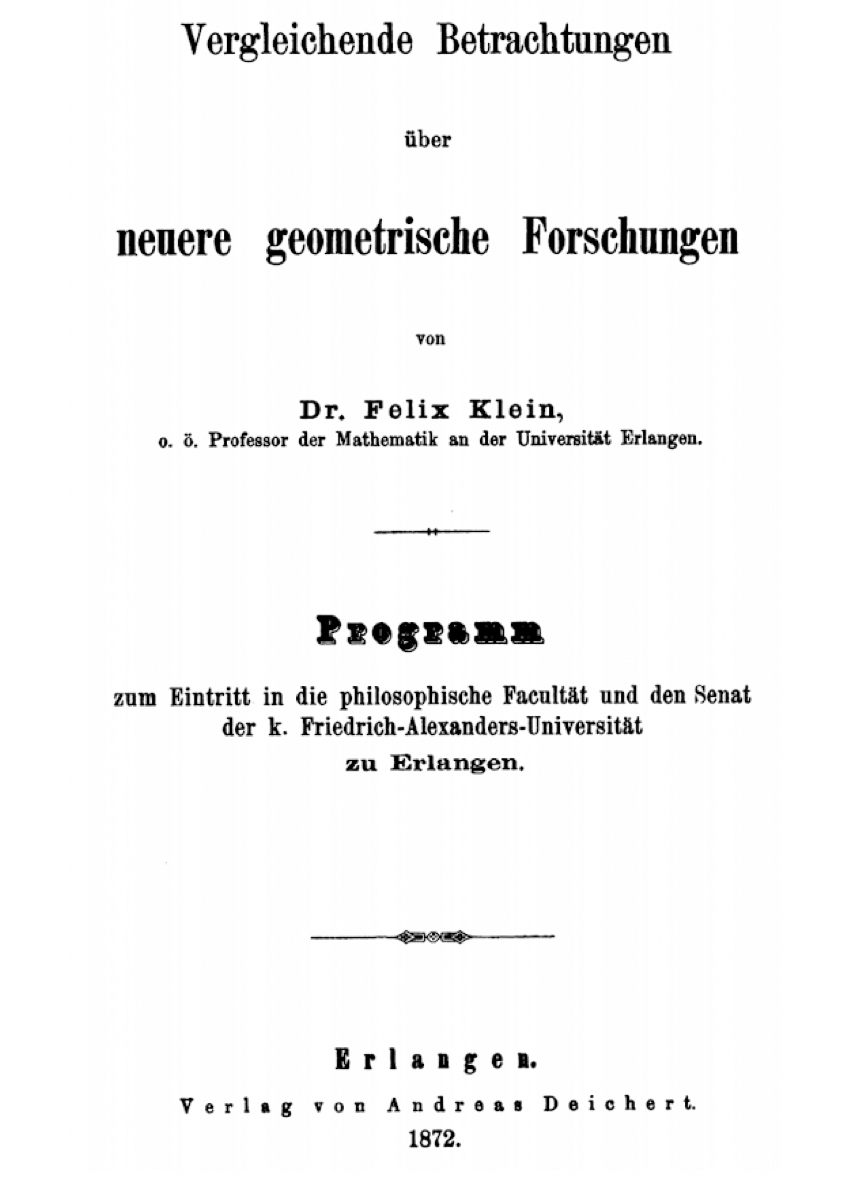
\includegraphics[width=0.9\linewidth]{figures/ml_erlangen.png}
一种广为流传的说法认为，Klein 于 1872 年 10 月在就职演说中提出了 Erlangen Programme。Klein 的确做过这样一场演讲（不过是在同年 12 月 7 日），但听众并非数学界人士，内容也主要涉及他的数学教育思想。如今所谓的“Erlangen Programme”，实际上是他为教授任职所准备的研究计划小册子 {\em Vergleichende Betrachtungen über neuere geometrische Forschungen}（《新近几何研究的比较考察》）。见 \cite{tobies2019felix}。
%, subtitled {\em Programm zum Eintritt in die philosophische Fakultät und den Senat der k. Friedrich-Alexanders-Universität zu Erlangen} (``Program for entry into the Philosophical Faculty and the Senate of the Emperor Friedrich-Alexander University of Erlangen''). 
%While Erlangen claims the credit, Klein has stayed there for only three years, moving in 1875 to the Technical University of Munich (then called {\em Technische Hochschule}), followed by Leipzig (1880), and finally settling down in Göttingen from 1886 until his retirement. See R. Tobies, Felix Klein—Mathematician, Academic Organizer, Educational Reformer, In: H. G. Weigand et al. (eds) {\em The Legacy of Felix Klein}, Springer, 2019.
}一直与\emph{欧氏几何}同义，因为当时尚不存在其他类型的几何。
%
十九世纪，Lobachevesky、Bolyai、Gauss 和 Riemann 构造出非欧几何的实例，Euclid 的垄断由此终结。
%
%By the late nineteenth century however, various alternative non-Euclidean geometries such as hyperbolic-, elliptic- and projective geometry had emerged. 
%
到十九世纪末，这些研究已经分化为彼此迥异的领域；数学家和哲学家围绕各种几何的有效性、它们之间的关系以及“唯一真正的几何”究竟是什么展开争论。


年轻数学家 Felix Klein 为这一困境指出了出路；他于 1872 年受聘为巴伐利亚小城 Erlangen 的大学教授。在一份后来以\emph{Erlangen Programme} 载入数学史册的研究计划中，Klein 提议把几何视为对{\em 不变量}的研究，即在某类变换下保持不变的性质，而这类变换称为该几何的{\em 对称性}。
%and used the formalism of group theory. 
%
这种方法表明，当时已知的各种几何都可以通过适当选择对称变换来定义，并可用群论语言加以形式化，从而澄清了问题。
%
%understood as the study of those and only those properties that are invariant under some group of symmetries associated with the geometry.
例如，欧氏几何关注长度和角度，因为这些性质在欧氏变换群（旋转和平移）下保持不变；仿射几何则研究平行性，因为这一性质在仿射变换群下保持不变。
%
考察各自对应的群，这些几何之间的关系便一目了然：欧氏群是仿射群的子群，而仿射群又是射影变换群的子群。
%, so certain figures which are Euclidean-equivalent may not be affine- or projectively equivalent.


Erlangen Programme 对几何学产生了极其深远的影响。
此外，它的影响还扩展到其他领域，尤其是物理学：对称性原理使人们能够从对称性的第一性原理推导守恒定律（这一惊人成果称为 Noether 定理），
甚至能够把基本粒子分类为对称群的不可约表示。
%
{\em 范畴论}
%a formalization of abstract similarities between mathematical structures, 
如今已遍及纯数学；用其创立者 Samuel Eilenberg 和 Saunders Mac Lane 的话说，它可以“被视为 Klein 的 Erlangen Programme 的延续，因为带有变换群的几何空间被推广为带有映射代数的范畴”。\marginnote{见 \cite{marquis2009category}。}[2\baselineskip]


%In mathematics, the Erlangen program ultimately inspired the creation of categories by Eilenberg \& Mac Lane\footnote{Indeed, in the first paper on categories, the authors write that ``This may be regarded as a continuation of the Klein Erlanger Program, in the sense that a geometrical space with its group of transformations is generalized to a category with its algebra of mappings.''}, which are widely prized for their ability to bring forth abstract similarities between mathematical structures and to reveal many ideas as ``just'' a special case of a more general one.


在写作本文时，深度学习领域的状况在某种程度上令人联想到十九世纪的几何学。
针对各类数据的神经网络架构可谓琳琅满目，但统一性原则寥寥无几。
与过去一样，这使得人们难以理解各种方法之间的关系，并不可避免地导致同一概念在不同应用领域中被反复重新发明和包装。
%
对于试图学习这一领域的初学者而言，消化如此大量的重复思想无疑是一场噩梦。


本文尝试把 Erlangen Programme 的思想应用于深度学习领域，最终目标是对该领域进行系统化，并“贯通各个要点”。
%
我们把这一几何化尝试称为“几何深度学习”；秉承 Felix Klein 的精神，我们提出从对称性与不变性的第一性原理出发，推导不同的归纳偏置以及实现这些偏置的网络架构。
%
%more systematic understanding of the landscape of geometric deep learning methods.
%
具体而言，我们关注一大类用于分析非结构化集合、网格、图和流形的神经网络，并说明可以把它们统一理解为尊重这些域之结构与对称性的方法。
%
%The archetypes of these domains, grid, graphs, groups, and  `four G'


我们相信，本文会吸引广泛的深度学习研究者、实践者和爱好者。
%
初学者可以把它作为几何深度学习的概览和入门材料。
%
经验丰富的深度学习专家或许会发现从基本原理推导熟悉架构的新方法，以及一些出人意料的联系。
%
实践者或许能从中获得解决各自领域问题的新见解。


现代机器学习发展如此迅速，撰写这类文本的风险在于，它可能尚未问世就已过时并失去意义。由于本文着眼于基础，我们希望所讨论的关键概念能够超越其具体实现\marginnote{“掌握某些原理足以轻易弥补对某些事实的不了解。”\citep{helvetius1759esprit}}——或者用 Claude Adrien Helvétius 的话说，{\em ``la connaissance de certains principes supplée facilement à la connoissance de certains faits.'' }

%

\section*{记号}
\addcontentsline{toc}{section}{记号}
\sectionmark{记号}

\begin{minipage}{\textwidth}
\def\arraystretch{1.5}
\begin{tabular}{lp{3.25in}}
$\Omega,u$ & 域，域上的点\\
$x(u) \in \mathcal{X}(\Omega,\mathcal{C})$ & 域上的信号，形式为 $x:\Omega\rightarrow \mathcal{C}$\\
$f(x) \in \mathcal{F}(\mathcal{X}(\Omega))$ & 作用于域上信号的函数，形式为 $f:\mathcal{X}(\Omega) \rightarrow \mathcal{Y}$\\
%
$\fG,\fg$ & 群，群元素\\
$\fg.u, \rho(\fg)$ & 群作用，群表示\\
%
$\vec{X}\in\mathcal{C}^{|\Omega|\times s}$ & 表示离散域上信号的矩阵\\
$\vec{x}_u\in\mathcal{C}^{s}$ & 表示离散域信号 $\vec{X}$ 在元素 $u\in\Omega$ 上取值的向量\\
$x_{uj}\in\mathcal{C}$ & 表示第 $j$ 个分量的标量，该分量属于离散域信号 $\vec{X}$ 在元素 $u\in\Omega$ 上的取值\\
$\vec{F}(\vec{X})$ & 作用于离散域信号并以矩阵形式返回另一离散域信号的函数\\
%
$\tau:\Omega\rightarrow\Omega$ & 域的自同构\\
$\eta:\Omega\rightarrow\Omega'$ & 两个不同域之间的同构\\
$\sigma: \mathcal{C}\rightarrow\mathcal{C}'$ & 激活函数（逐点非线性）\\
%
$G=(\mathcal{V},\mathcal{E})$ & 具有节点 $\mathcal{V}$ 和边 $\mathcal{E}$ 的图\\
$\mathcal{T}=(\mathcal{V},\mathcal{E},\mathcal{F})$ & 具有节点 $\mathcal{V}$、边 $\mathcal{E}$ 和面 $\mathcal{F}$ 的网格\\
%
$x\star \theta$ & 与滤波器 $\theta$ 的卷积\\
$S_v$ & 移位算子\\
%
$\varphi_i$ & 基函数\\
%
%
$T_u\Omega, T\Omega$ & $u$ 处的切空间，切丛\\
$X \in T_u\Omega$ & 切向量\\
$g_u(X,Y) = \langle X, Y\rangle_u$ & Riemann 度量\\
%
$\ell(\gamma), \ell_{uv}$ & 曲线 $\gamma$ 的长度，边 $(u,v)$ 上的离散度量\\

\end{tabular}
\end{minipage}
\pagebreak


\section{引言}                % Print a "chapter" heading

过去十年见证了数据科学与机器学习领域的一场实验革命，其典型代表是深度学习方法。事实上，许多过去被认为遥不可及的高维学习任务——例如计算机视觉、围棋对弈或蛋白质折叠——在具备适当计算规模时确实可以实现。
%
值得注意的是，深度学习的本质建立在两条简单的算法原则之上：
第一是表示学习或\emph{特征学习}的概念，即用经过适配且通常具有层次结构的特征来捕获适合各项任务的正则性；第二是通过局部梯度下降进行学习，通常实现为{\em 反向传播}。%, such as gradient descent.

尽管在高维空间中学习一般函数是一个受维数灾难困扰的估计问题，但多数值得关注的任务并非一般问题，而是带有由物理世界内在低维性与结构所产生的重要预定义正则性。本文旨在通过统一的几何原则揭示这些正则性，而这些原则可以应用于广泛的应用场景。

利用大型系统中已知的对称性，是对抗维数灾难的一种强有力且经典的方法，也是多数物理理论的基础。深度学习系统也不例外；从早期开始，研究者便对神经网络进行调整，以利用物理测量产生的低维几何，例如图像中的网格、时间序列中的序列，或分子中的位置与动量，以及与之相关的平移、旋转等对称性。
在全文论述中，我们将把这些模型以及许多其他模型描述为同一底层几何正则性原则的自然实例。%stability.

这种秉承 Erlangen Programme 精神的“几何统一”尝试
%--our own Erlangen Program
%\marginnote{We are mindful that the risk of flashy buzzwords such as {\em The Hilbert Problems of X} or {\em Erlangen Program of Y} inevitably implies the irreverent analogy between ourselves and the aforementioned giants. Our only intent here is to draw inspiration from Klein's approach -- {\em ergo, parce nobis, benevole lector!}
%} -- 
具有双重目的：一方面，它为研究 CNN、RNN、GNN 和 Transformer 等最成功的神经网络架构提供了统一的数学框架；另一方面，它给出一种把物理先验知识纳入神经架构的构造性过程%， an essential ingredient to improve the sample efficiency of data-driven methods into computational sciences
，并为构建尚待发明的未来架构提供有原则的方法。

在继续之前，需要指出的是，我们的工作关注\emph{表示学习架构}以及如何在其中利用数据的对称性。可以使用这类表示的众多精彩\emph{流水线}（例如自监督学习、生成建模或强化学习）\emph{并非}本文的核心重点\marginnote{用于\emph{优化}或\emph{正则化}架构的技术亦是如此，例如 Adam \citep{kingma2014adam}、dropout \citep{srivastava2014dropout} 或批归一化 \citep{ioffe2015batch}。}。因此，我们不会深入综述变分自编码器 \citep{kingma2013auto}、生成对抗网络 \citep{goodfellow2014generative}、归一化流 \citep{rezende2015variational}、深度 Q 网络 \citep{mnih2015human}、近端策略优化 \citep{schulman2017proximal} 或深度互信息最大化 \citep{hjelm2018learning} 等有影响力的神经网络流水线。尽管如此，我们相信本文所关注的原则在所有这些领域中都具有重要意义。
%having good foundations on exploiting the geometry of data will lead to successes when the resulting neural architectures are plugged into any of the above pipelines.

此外，为了展示几何蓝图的力量，我们虽然力求覆盖相当广泛的范围，但并不试图精确概括几何深度学习领域\emph{全部}丰富的既有研究。相反，我们深入研究若干著名架构，以展示这些原则并将其建立在既有研究基础上；同时希望留下足够的参考文献，使读者能够有意义地把这些原则应用于今后遇到或设计的任何几何深度架构。

%\raggedbottom
\section{高维空间中的学习}

%\textbf{[Summarise this section into the main elements here, with less formality]}


% Main points to illustrate:
% \begin{itemize}
%     \item Modern High-dimensional learning as interpolation. Choosing regularity prior for interpolant in high-dimensions? 
%     \item In low-dimensions, we have good notions of regularity (Sobolev, Holder, etc. ). 
%     \item These can be extended to high-dimensions using reproducing kernel hilbert spaces, or Lipschitz classes. They all suffer from a curse of dimensionality, consequence of the fact that no structural assumptions are made on the data domain. 
%     \item Functions parametrised as neural networks? 
    
% \end{itemize}

在最简单的形式化中，监督式机器学习考虑一组 $N$ 个观测 $\gD=\{(x_i, y_i)\}_{i=1}^{ N}$，它们从底层数据分布 $P$ 中\emph{独立同分布地}抽取；该分布定义于 $\gX \times \gY$ 上，其中 $\gX$ 和 $\gY$ 分别为数据域和标签域。这一设置的决定性特征在于，$\gX$ 是一个{\em 高维空间}：通常假设 $\gX= \R^d$ 是维数 $d$ 很大的欧氏空间。

%In our context, however, $\gX$ will often take a more structured form, such as the space of functions $\gX(\Omega) = \{ x: \Omega \to \R \}$ defined over a low-dimensional domain $\Omega$, which can be a geometric object such as a grid, manifold, or a graph. 

进一步假设标签 $y$ 由某个未知函数 $f$ 生成，使得 $y_i = f(x_i)$，
那么学习问题便归结为估计函数 $f$，所使用的参数化函数类为 $\gF=\{ f_{\thetab \in \Theta}\}$。神经网络是这类参数函数类的一种常见实现，此时 $\thetab \in \Theta$ 对应网络权重。
%e.g. to the weights of a neural network. 
在这一理想化设置中，标签不含噪声；现代深度学习系统通常工作在所谓的\emph{插值状态}下，其中估计得到的 $\tilde{f} \in \gF$ 满足 $\tilde{f}(x_i) = f(x_i)$，且这一条件适用于所有 $i=1,\hdots, N$。
学习算法的性能以从 ${P}$ 抽取的新样本上的\emph{期望性能}\marginnote{统计学习理论关注基于{\em 集中不等式}的更精细泛化概念；我们将在未来工作中回顾其中一些概念。}来衡量，并使用某种{\em 损失} $L(\cdot,\cdot)$：
$$\gR(\tilde{f}):= \mathbb{E}_{P}\,\, L(\tilde{f}(x), f(x)),$$
%
其中平方损失 $L(y,y')=\frac{1}{2}|y-y'|^2$ 是最常用的损失之一。


因此，成功的学习方案需要为 $f$ 编码适当的正则性概念或\emph{归纳偏置}，并通过构造函数类 $\mathcal{F}$ 和使用{\em 正则化}来施加这种偏置。下一节将简要介绍这一概念。%, and will explore it in detail in follow-up work.


\subsection{通过函数正则性引入归纳偏置}
\label{sec:inductive}


现代机器学习使用规模庞大、质量很高的数据集；这些数据集连同适当的计算资源，促使人们设计丰富的函数类 $\gF$，使其具有对这类大规模数据进行插值的能力。
%
这种
%non-parametric % Taco: can we really call this "non-parametric"? It's just a very large parametric function space, no?
思路与神经网络十分契合，因为即使选择最简单的架构，也会得到一个{\em 稠密}函数类。\marginnote{若集合 $\mathcal{A}\subset \mathcal{X}$ 在 $\mathcal{X}$ 中稠密，则其闭包满足
$$
\mathcal{A}\cup \{ \displaystyle \lim_{i\rightarrow \infty} a_i : a_i \in \mathcal{A}\} = \mathcal{X}.
$$ 
这意味着 $\mathcal{X}$ 中任意点都可以任意接近 $\mathcal{A}$ 中的某个点。典型的通用逼近结果表明，例如由双层感知机 $f(\mathbf{x}) = \mathbf{c}^\top\mathrm{sign}(\mathbf{A}\mathbf{x}+\mathbf{b})$ 表示的函数类，在 $\mathbb{R}^d$ 上的连续函数空间中稠密。
} 
%
逼近几乎任意函数的能力
%\marginnote{More precisely, Borel-measurable. } 
是各种\emph{通用逼近定理}的研究主题；二十世纪九十年代，应用数学家和计算机科学家证明并推广了若干此类结果（例如见 \cite{cybenko1989approximation,hornik1991approximation,barron1993universal,leshno1993multilayer,maiorov1999best,pinkus1999approximation}）。
%(Barron, Meir, Maiorov, Pinkus, Cybenko, Hornik, etc.) 

\begin{figure}[h!]
    \centering
    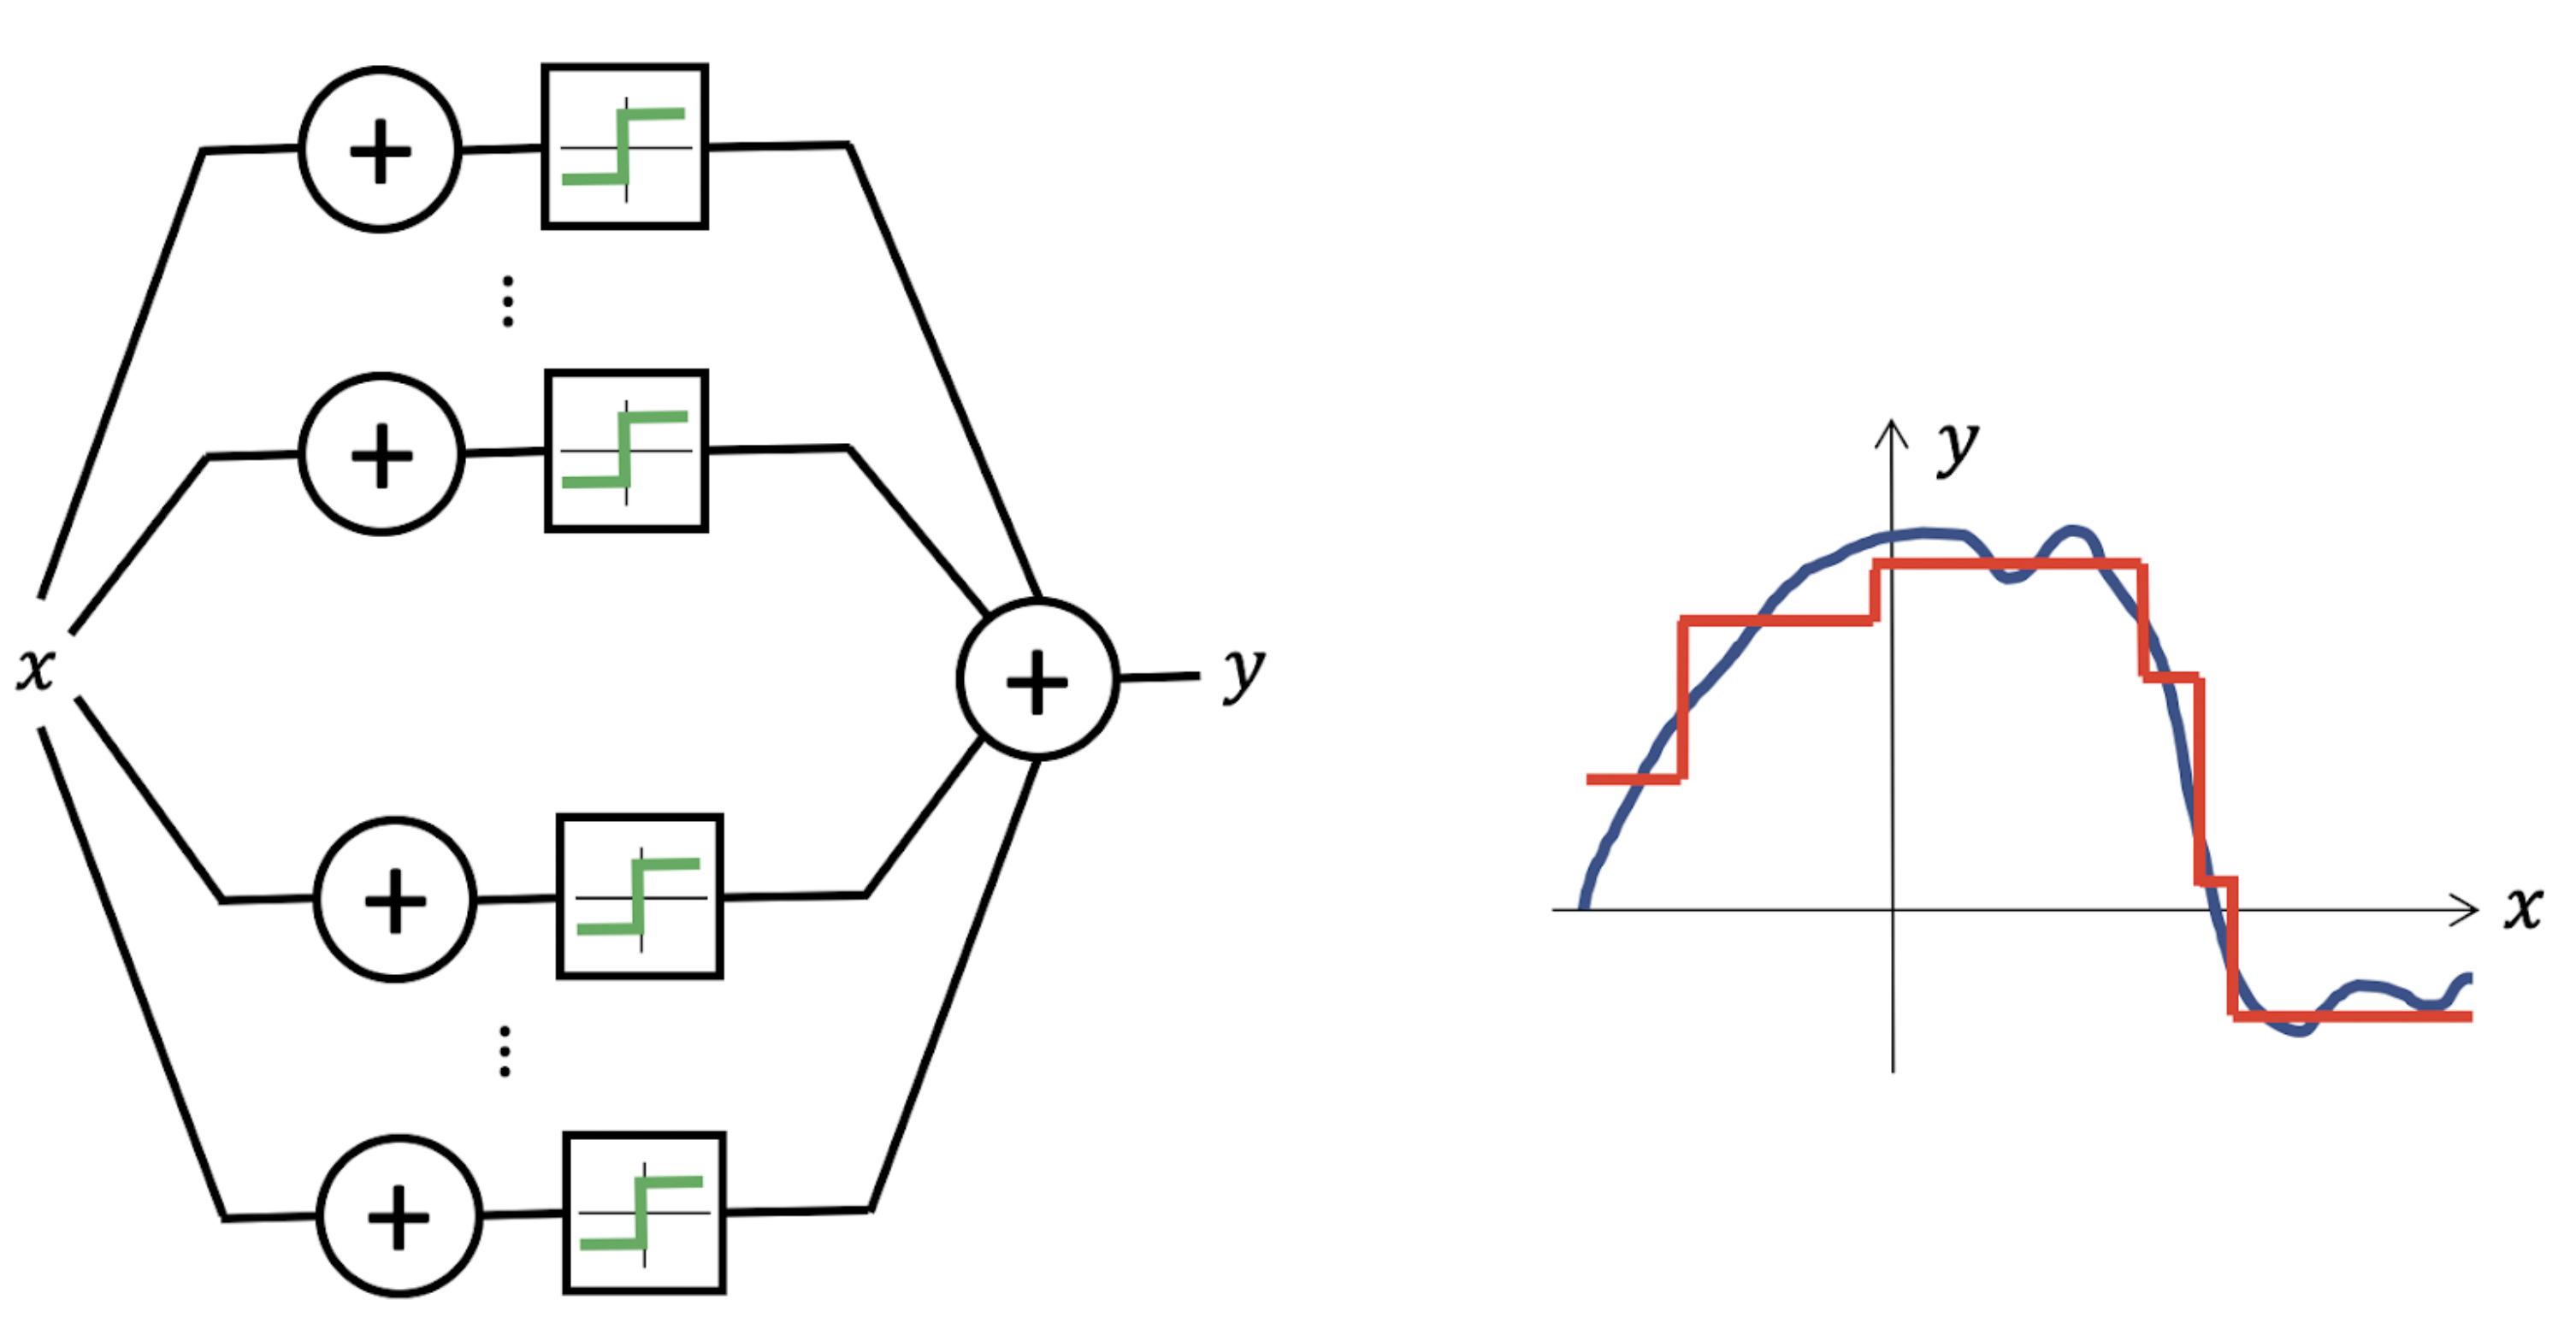
\includegraphics[width=1\linewidth]{figures/ua_mlp.png}
    \caption{多层感知机 \citep{rosenblatt1958perceptron} 是最简单的前馈神经网络，也是通用逼近器：仅使用一个隐藏层，它们就能表示阶跃函数的组合，从而以任意精度逼近任何连续函数。}
    \label{fig:ua_mlp}
\end{figure}%


%\michael{Show an intuitive example of MLP approximating step functions}


然而，通用逼近并不意味着归纳偏置{\em 不存在}。给定具有通用逼近能力的假设空间 $\gF$，可以定义复杂度度量 $c: \gF \to \R_{+}$，并把插值问题重新定义为
$$
\tilde{f} \in \arg\min_{g \in \gF} c(g) \quad \mathrm{s.t.} \quad g(x_i) = f(x_i)  \quad \mathrm{for} \,\,\, i=1, \hdots, N,
$$
也就是说，我们要在假设类中寻找最为正则的函数。
%
对于标准函数空间，这种复杂度度量可以定义为{\em 范数}，\marginnote{
%A {\em norm} is a non-negative function $\| \cdot \|$ on a vector space that is {\em homogeneous} $\| \alpha x \| = |\alpha| \| x\|$, {\em subadditive} $\|x+y \| \leq \|x\| + \|y\|$ and {\em positive-definite} $\|x\|=0 \Rightarrow x=0$. 
非正式地说，范数 $\|x\|$ 可以视为向量 $x$ 的“长度”。
{\em Banach 空间}是配备范数的完备向量空间。
}从而使 $\gF$ 成为{\em Banach 空间}，并能够利用泛函分析中的大量理论结果。
%
在低维空间中，样条是函数逼近的主力工具。它们可以按上述方式表述，并用范数捕获经典的光滑性概念，例如三次样条的二阶导数平方范数 $\int_{-\infty}^{+\infty} |f''(x)|^2 \mathrm{d}x$。

%\michael{Notation: change complexity from $\gamma$ to $c$ (which we used for Dirichlet)?}


对于神经网络，复杂度度量 $c$ 可以用网络权重表示，即 $c(f_{\boldsymbol{\theta}}) = {c}(\boldsymbol{\theta})$。
%
网络权重的 $L_2$ 范数（称为\emph{权重衰减}）或所谓的\emph{路径范数} \citep{neyshabur2015norm}，都是深度学习文献中的常见选择。
%\michael{I suggest we give concrete examples here, e.g. sparsity-inducing regularization and low-dimensional projections}
%
%
从 Bayesian 视角看，这类复杂度度量也可以解释为目标函数先验的负对数。更一般地，可以把这种复杂度纳入经验损失，从而\emph{显式地}施加它（得到所谓的结构风险最小化）；也可以使其作为某种优化方案的结果而\emph{隐式地}施加。例如，众所周知，对欠定最小二乘目标执行梯度下降，会选择具有最小 $L_2$ 范数的插值解。将这类隐式正则化结果推广到现代神经网络，是当前研究的主题（例如见 \cite{blanc2020implicit, shamir2020implicit, razin2020implicit, gunasekar2017implicit}）。
总而言之，一个自然的问题随之产生：如何定义有效先验，以捕获现实世界预测任务中预期的正则性与复杂度？
%We will address this question in Chapter ??




\subsection{维数灾难}

低维空间中的插值%$\gX = \R^d$
（其中 $d=1,2$ 或 $3$）是一项经典的信号处理任务；借助日益精细的正则性类别（例如样条插值、小波、曲波或脊波），可以对估计误差进行非常精确的数学控制。然而，高维问题的情形截然不同。
%

% \begin{figure}[h!]
%     \centering
%     %\includegraphics[width=0.3\linewidth]{figures/curseofdim1.pdf}
%     \caption{An $\epsilon$-net of a  $d$-dimensional Euclidean domain of diameter $1$ grows exponentially as $\epsilon^{-d}$. }
%     \label{fig:curseofdim}
% \end{figure}%

%\michael{We need to clean up notation: in ML problems our main object is $f(x)$ where $x$ is the input, e.g. an image. It has its own structure, being in own turn a signal on the domain, $x(u)$.}

为了说明这一思想的本质，考虑一种易于推广到高维空间的经典正则性概念：1-Lipschitz 函数 $f:\mathcal{X} \to \R$，即满足 $|f(x) - f(x')| \leq \|x - x'\|$ 的函数，而这一条件适用于所有 $x, x' \in \mathcal{X}$。该假设只要求目标函数在\emph{局部}光滑；也就是说，如果输入 $x$ 只受到轻微扰动（由范数 $\|x - x'\|$ 衡量），输出 $f(x)$ 就不能发生太大变化。%\michael{Lets avoid confusion and use $\mathcal{X}$ rather than $\Omega$}
%\marginnote{The number of protons in the observable universe, known as the {\em Eddington number}, is currently estimated at $\sim 10^{80}$.}
如果关于目标函数 $f$ 的唯一已知信息是它满足 $1$-Lipschitz 条件，那么需要多少观测才能保证估计 $\tilde{f}$ 接近 $f$？
图 \ref{fig:curseofdim} 表明，一般答案必然随维数 $d$ 指数增长，这说明随着输入维数增加，Lipschitz 类增长得“过快”：在许多维数 $d$ 甚至并不很大的应用中，所需样本数也会超过宇宙中的原子数。
如果把 Lipschitz 类替换为全局光滑性假设，例如 Sobolev 类 $\gH^{s}(\Omega_d)$，情况也不会改善\marginnote{若函数 $f$ 属于{\em Sobolev 类} $\gH^{s}(\Omega_d)$，则 $f \in L^2(\Omega_d)$，且其广义 $s$ 阶导数平方可积，即 $\int |\omega|^{2s+1} |\hat{f}(\omega)|^2 d\omega < \infty$，其中
$\hat{f}$ 是 $f$ 的 Fourier 变换；见第~\ref{sec:grids_euclidean} 节。
}。事实上，经典结果 \citep{tsybakov2008introduction} 给出了 Sobolev 类数量级为 $\epsilon^{-d/s}$ 的逼近与学习极小极大速率，说明对 $f$ 施加额外光滑性假设，只有在 $s \propto d$ 时才能改善统计情形，而这一假设在实践中并不现实。

% on the one hand, `globally' smooth functions, with $s$-order derivatives \marginnote{The \emph{Sobolev} class defines  }

% In fact, even though we can extend the above `classic' functional spaces to arbitrary dimensions, they suffer from the so-called \emph{curse of dimensionality}. In essence, in order to obtain an expected generalization error $\mathbb{E}_{x\sim \mathbb{P}} | \tilde{f}(x) - f(x)| \leq \epsilon$, such regularity hypotheses require an order of $\epsilon^{-d}$ observations, signalling an impossibility of efficient learning : in many applications with even modest dimension $d$, the number of samples would be bigger than the number of atoms in the universe.
% \marginnote{The number of protons in the observable universe, known as the Eddington number, is currently estimated at $\sim 10^{80}$.}

\begin{figure}[h!]
    \centering
%    \includegraphics[width=0.45\linewidth]{figures/curseofdim4.pdf} 
 %       \includegraphics[width=0.45\linewidth]{figures/curseofdim2.pdf}
       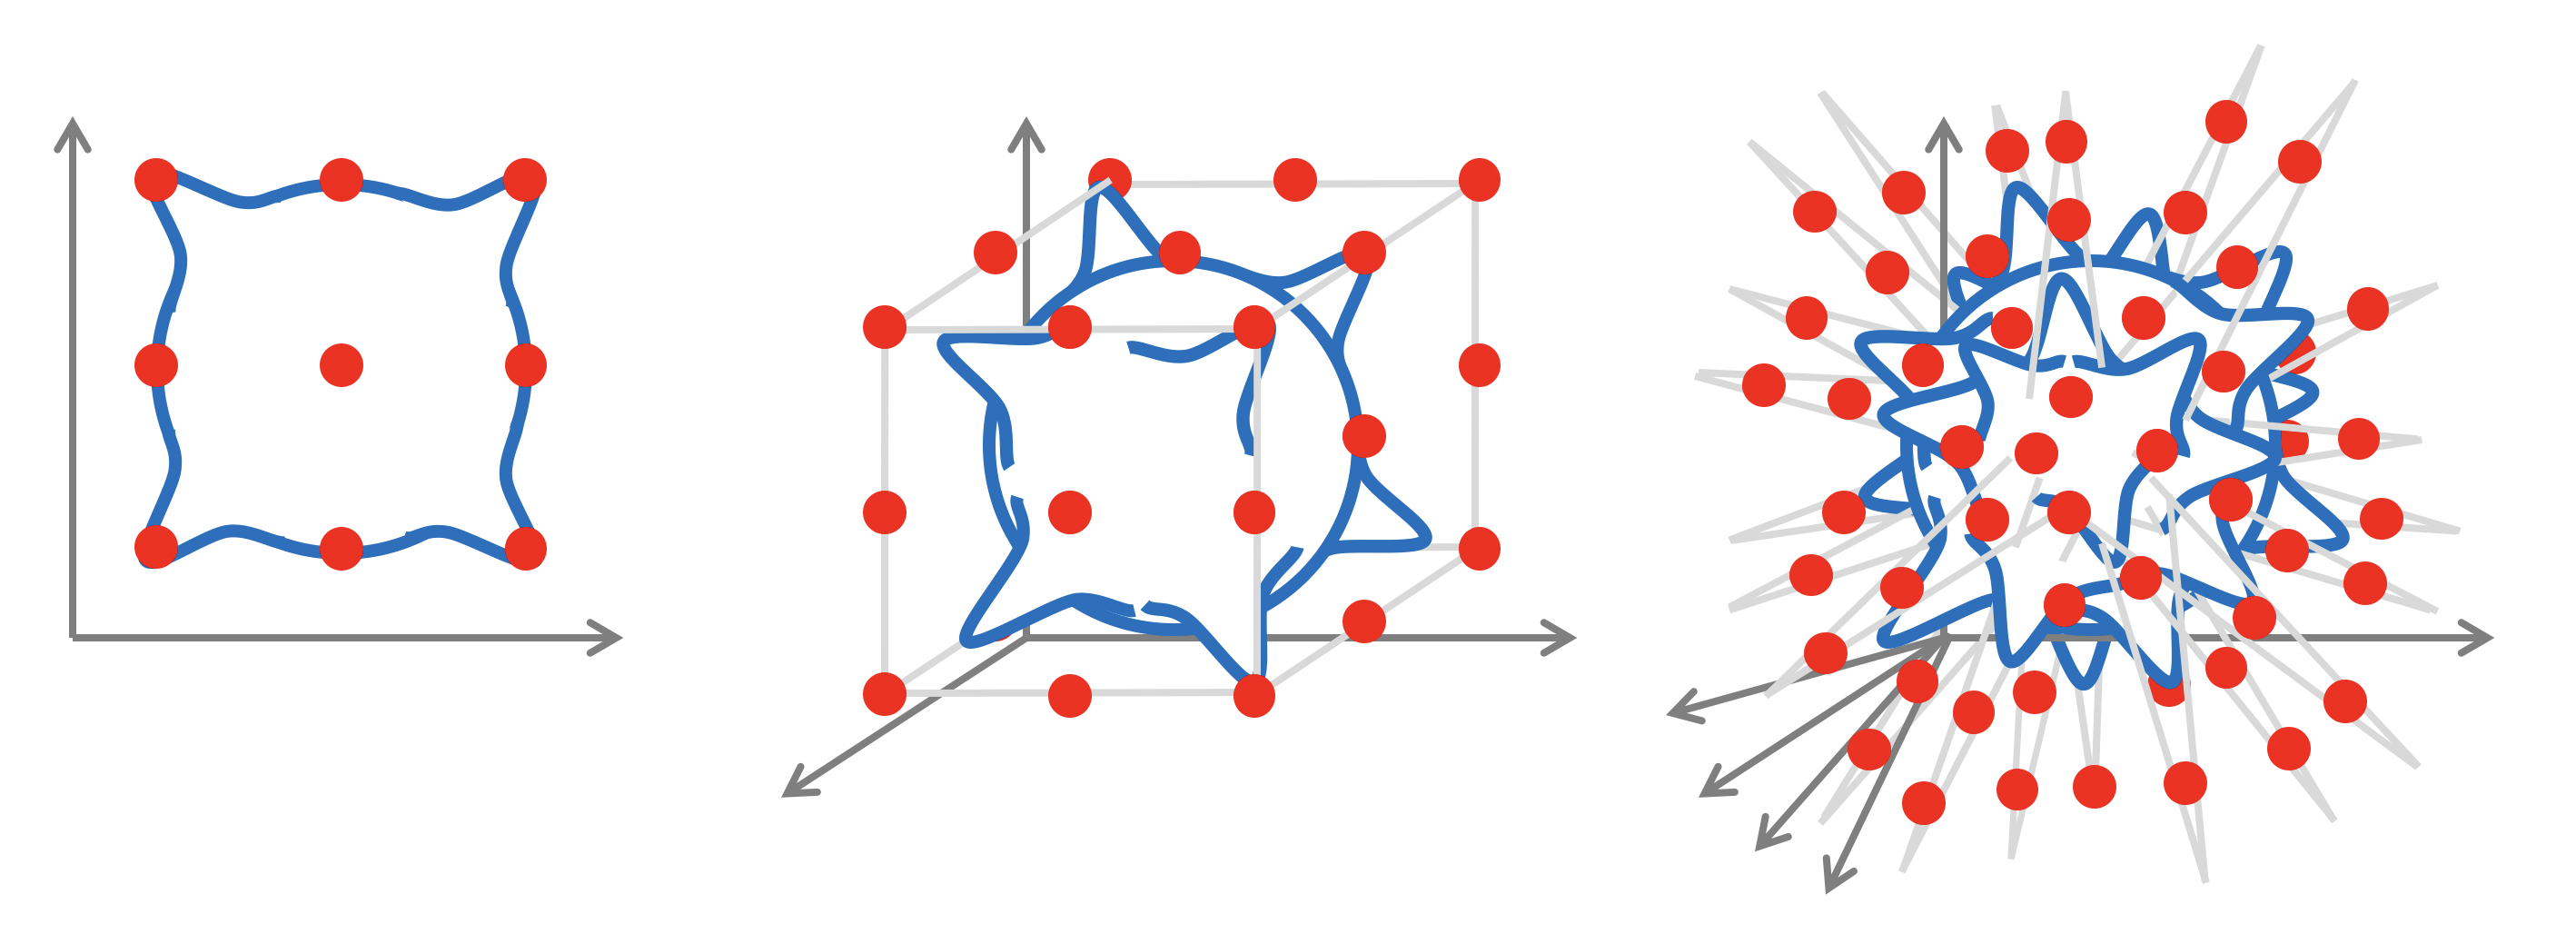
\includegraphics[width=\linewidth]{figures/blobs.png} 
    \caption{考虑 Lipschitz 函数 $f(x) = \sum_{j=1}^{2^d} z_j \phi(x-x_j)$，其中 $z_j=\pm 1$，每个象限放置一个 $x_j \in \R^d$，而 $\phi$ 是具有局部支撑的 Lipschitz 隆起函数。除非在 $2^d$ 个象限中的大多数象限内观测该函数，否则对它的预测将产生常数误差。这一简单的几何论证可以通过\emph{最大差异} \citep{von2004distance} 的概念形式化；对 Lipschitz 类，它定义为 $\kappa(d)=\mathbb{E}_{x,x'} \sup_{f \in \mathrm{Lip}(1)} \left| \frac{1}{N}\sum_{l} f(x_l) - \frac{1}{N}\sum_{l} f(x'_l) \right| \simeq N^{-1/d}$，用于衡量两个独立 $N$ 样本期望之间最大的期望差异。要保证 $\kappa(d) \simeq \epsilon$，需要 $N = \Theta(\epsilon^{-d})$；相应样本 $\{x_l\}_l$ 定义了该域的一个 $\epsilon$-网。对于 $d$ 维、直径为 $1$ 的欧氏域，其大小按 $\epsilon^{-d}$ 指数增长。}
    \label{fig:curseofdim}
\end{figure}


%\michael{\bf [MB: INSERT FIGURE and explain the curse of dimensionality as a geometric phenomenon using the volume of inscribed unit ball]}


%\michael{\bf [MB: General comment: in order not to interrupt the flow, we can have self-contained figures with long captions or `inserts' explaining important concepts. We had it in our Signal Processing Magazine paper and it was a very good idea
%}

%\joan{Agreed. The Curse of Dimensonality could be one such insert, with a panel with (i) a figure that displays the exponential dependence of epsilon-grids wrt dimension, and caption. TODO JOAN}

全连接神经网络定义的函数空间可以表达更灵活的正则性概念，这是通过在其权重上考虑复杂度函数 $c$ 得到的。具体而言，通过选择促进稀疏性的正则化，它们能够打破这种维数灾难 \citep{bach2017breaking}。然而，代价是必须对目标函数 $f$ 的性质作出强假设，例如假设 $f$ 依赖于输入的一组低维投影（见图 \ref{fig:curseofdim2}）。
%\michael{\bf [MB: not sure I understand this part. Isn't there a universal approximation result?]} \joan{I further clarified}
在多数现实应用中（例如计算机视觉、语音分析、物理学或化学），目标函数%$f$
往往表现出无法用低维投影表达的复杂长程相关性（图 \ref{fig:curseofdim2}），因而这一假设并不现实。
因此，有必要通过利用物理域的空间结构以及 $f$ 的几何先验，定义另一种正则性来源，具体将在下一节~\ref{sec:geom_priors} 中说明。

\begin{figure}[htbp]
    \centering
%    \includegraphics[width=0.45\linewidth]{figures/curseofdim5.pdf} 
%    \includegraphics[width=0.45\linewidth]{figures/mnistm.pdf} %
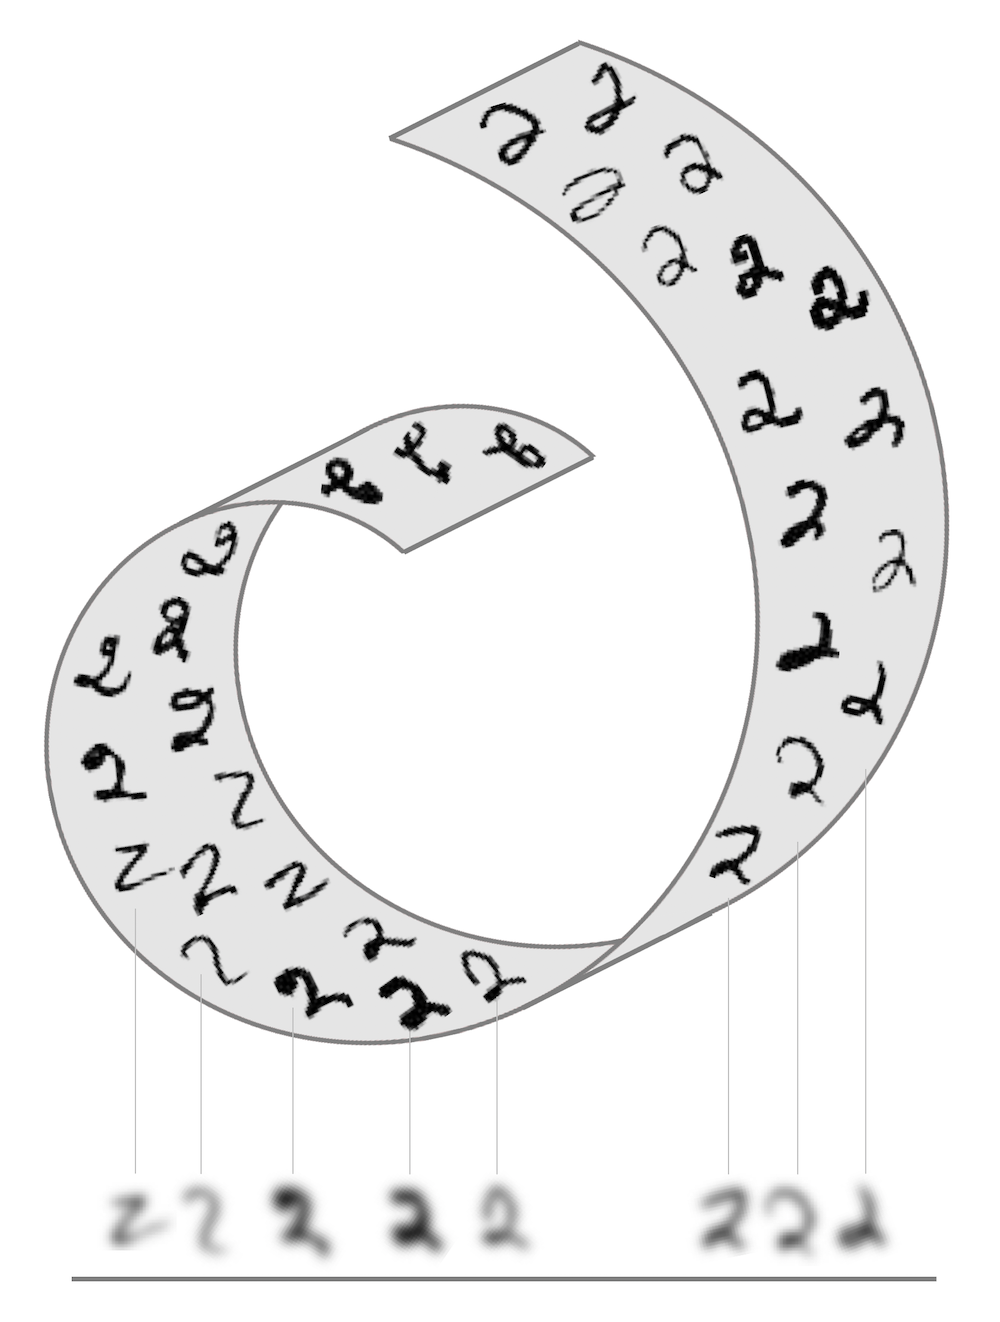
\includegraphics[width=0.6\linewidth]{figures/mnist.png}
    \caption{%\michael{Lets not use $\Omega$ here but $\mathcal{X}$ as the domain of $f$} 
    如果假设未知函数 $f$ %:\gX \to \R$
    可以由 $f(\mathbf{x}) \approx g(\mathbf{A}\mathbf{x})$ 良好逼近，其中某个未知的 $\mathbf{A} \in \mathbb{R}^{k \times d}$ 满足 $k \ll d$，那么浅层神经网络可以捕获这种归纳偏置，例如见 \cite{bach2017breaking}。在典型应用中，这种对低维投影的依赖并不现实，如本例所示：低通滤波器把输入图像投影到低维子空间；虽然它传达了大部分语义，却丢失了大量信息。%\michael{Joan: why not to show the Swiss-roll surface?} \joan{Yes, we can use it to replace the sketch in the left. }
    % Taco: is the blurred MNIST really a good example? I guess that if we used a PCA projection we could keep >98% of the variance with only a few components for this dataset. But perhaps for natural images this is no longer true..
    }
    \label{fig:curseofdim2}
\end{figure}


\newpage
\section{几何先验}
\label{sec:geom_priors}
现代数据分析几乎等同于高维学习。
尽管第~\ref{sec:inductive} 节中的简单论证表明，由于维数灾难，不可能从一般高维数据中学习，
但对于具有物理结构的数据仍有希望，因为我们可以采用两条基本原则：{\em 对称性}与{\em 尺度分离}。
在本文所考虑的设置中，这种附加结构通常来自输入信号底层域的结构：
我们将假设机器学习系统作用于某个域 $\Omega$ 上的\emph{信号}（函数）。
%
尽管在许多情况下，$\Omega$ 上点的线性组合并没有良好定义\marginnote{$\Omega$ 必须是向量空间，表达式 $\alpha u + \beta v$ 才有意义。}，但我们可以对其上的信号作线性组合；也就是说，信号空间构成一个向量空间。
此外，由于可以定义信号之间的内积，该空间是一个{\em Hilbert 空间}。

\begin{tcolorbox}[width=\linewidth,
                  boxsep=0pt,
                  left=7.5pt,
                  right=7.5pt,
                  top=7.5pt,
                  bottom=7.5pt,
                  arc=0pt,
                  boxrule=0pt,toprule=0pt,
                  colback=boxgray,
                  ]%%

取值于 $\mathcal{C}$、定义在 $\Omega$ 上的信号空间
\marginnote{当 $\Omega$ 具有某种附加结构时，可以进一步限制 $\mathcal{X}(\Omega, \mathcal{C})$ 中信号的类型。例如，当 $\Omega$ 是光滑流形时，可以要求信号光滑。
为简洁起见，只要不会引起歧义，我们将省略值域 $\mathcal{C}$。
} %can impose smoothness on the signals.}% For instance, when $\Omega$ is a smooth manifold we may require signals in $\mathcal{X}(\Omega, \mathcal{C})$ to be smooth.}
（其中 $\Omega$ 是一个可能具有附加结构的集合，$\mathcal{C}$ 是一个向量空间，其维度称为\emph{通道}）
\begin{equation}
    \mathcal{X}(\Omega, \mathcal{C}) = \{ x : \Omega \rightarrow \mathcal{C} \}
\end{equation}
%
是一个具有向量空间结构的函数空间。
%In particular, it satisfies the distributivity property 
信号的加法与标量乘法定义为：
\begin{equation*}
    (\alpha x + \beta y)(u) = \alpha x(u) + \beta y(u) \quad \text{for all} \quad u\in \Omega,
\end{equation*}
其中 $\alpha, \beta$ 为实标量。% are vectors, and $u \in \Omega$.
%
给定内积 $\langle v, w \rangle_\mathcal{C}$（定义在 $\mathcal{C}$ 上）以及测度\marginnote{当域 $\Omega$ 是离散的时，可以选择 $\mu$ 为{\em 计数测度}，此时积分变为求和。下文将省略测度，并为简洁起见使用 $\mathrm{d}u$。}$\mu$（定义在 $\Omega$ 上，并可据此定义积分），就可以在 $\mathcal{X}(\Omega, \mathcal{C})$ 上定义如下内积：
\begin{equation}
    \langle x, y \rangle = \int_{\Omega} \langle x(u), \, y(u) \rangle_{\mathcal{C}} \; \mathrm{d}\mu(u).
    \label{eqn:innerprod}
\end{equation}
\end{tcolorbox}

%we will assume that $f$ operates on $\mathcal{C}$-valued signals $\mathcal{X}(\Omega, \mathcal{C}) = \{x: \Omega \rightarrow \mathcal{C} \}$, where $\Omega$ is some input domain and $\mathcal{C}$ is a vector space, typically $\mathcal{C} = \R^s$ for a signal with $s$ channels.
%\marginnote{For the sake of simplicity, we will often assume scalar-valued signals, i.e., $s=1$. }
%We note that $\mathcal{X}(\Omega, \mathcal{C})$ is a vector space, with addition and scalar multiplication defined pointwise (i.e. $(f + f')(x) = f(x) + f(x')$ and $(\alpha f)(x) = \alpha f(x)$).

作为一个典型示例，令 $\Omega = \mathbb{Z}_n\times \mathbb{Z}_n$ 为二维 $n\times n$ 网格，令 $x$ 为 RGB 图像（即信号 $x : \Omega \rightarrow \R^3$），并令 $f$ 为作用于 $3n^2$ 维输入的函数（例如单层感知机）。
%
正如下文将更详细说明的，域 $\Omega$ 通常配备某种几何结构与对称性。%symmetric structure (in our example, rotational and translational symmetry) that is manifested both in signals $x$ defined on this domain as well as in functions $f$ acting on such signals.
%
尺度分离源于这样一种能力：把信号转移到较粗糙版本的域上时，仍能保留信号的重要特征（在本例中，即通过粗化底层网格对图像进行下采样）。


我们将说明，这两条原则——统称为{\em 几何先验}——在多数现代深度学习架构中都十分突出。对于上述图像情形，几何先验通过共享权重的卷积滤波器（利用平移对称性）和池化（利用尺度分离）被内置于卷积神经网络（CNN）中。
%
把这些思想推广到图、流形等其他域，并说明几何先验如何从基本原则中产生，是几何深度学习的主要目标，也是本文的{\em 主旋律}。



\subsection{对称性、表示与不变性}
\label{sec:symmetries}

%Symmetries are a foundational principle of physics, providing a strong constraint on the form of physical laws.
%In the context of machine learning, symmetries also provide key regularity priors that allow to break the curse of dimensionality and enable efficient high-dimensional learning. 

非正式地说，对象或系统的{\em 对称性}是一种使该对象或系统的某种性质保持不变，即保持{\em 不变性}的变换。
这类变换可以是光滑的、连续的或离散的。
%A canonical example for continuous symmetries in physics is Lagrangian mechanics, which states that the laws of motion are preserved under rigid transformations of the observer's point of view. 
%
对称性普遍存在于许多机器学习任务中。
例如，在计算机视觉中，物体类别不随平移而改变，因此平移是视觉物体分类问题中的对称性。
%one is often interested in classifying  objects in images independently of their position, a setting referred to as {\em translation invariant}. 
%
%classification through translation invariance, or 
在计算化学中，要在不依赖分子空间取向的情况下预测分子性质，需要{\em{旋转不变性}}。
%
在描述粒子没有典范次序、因而可以任意置换的粒子系统时，离散对称性会自然出现；在许多动力系统中，离散对称性也会通过时间反演对称性自然出现
%through permutations, 
%or also 
（例如满足细致平衡的系统或 Newton 第二运动定律）。%\marginnote{ADD COMMENT on Newton's law} % may not be necessary imo
%
正如第~\ref{sec:proto-graphs} 节将看到的，置换对称性也是分析图结构数据的核心。% and will be a prominent topic in this book.

\paragraph{对称群}
一个对象的对称性集合满足若干性质。
%which make this set into an algebraic structure called a \emph{symmetry group}.
%Symmetries lend themselves to a rich and powerful mathematical characterization.
%More specifically, the set of symmetries of a given object forms an algebraic object called a symmetry group.
首先，可以组合对称性来得到新的对称性：如果 $\fg$ 和 $\fh$ 是两个对称性，
%transformations of a system that leave it unchanged, 
那么它们的复合 $\fg \circ \fh$ 和 $\fh \circ \fg$
%\marginnote{From hereon we will denote composition of group elements by $\fg \fh$, leaving out the $\circ$ symbol.}
\marginnote{我们将遵循群论中使用的并置记号约定 $\fg \circ \fh = \fg \fh$；它应从右向左读，即先应用 $\fh$，再应用 $\fg$。次序十分重要，因为许多情况下对称性不满足交换律。
%
熟悉 Lie 群的读者可能会对我们使用 Fraktur 字体表示群元素感到不习惯，因为这种字体通常用于表示 Lie 代数。
}也仍然是对称性。
原因在于，如果两个变换都使对象保持不变，那么它们的复合也具有这一性质，因此该复合仍是对称性。
%\marginnote{This property is called {\em closure} in group theory.} 
此外，对称性总是可逆的，并且其逆仍是对称性。
%Together with {\em associativity} $(\fg \circ \fh) \circ \ff = \fg \circ (\fh \circ \ff)$ of the composition operation and existence of unique {\em identity} ($\exists!\fe \in \fG$ such that $\fe \circ \fg = \fg \circ \fe = \fe$ for all $\fg \in \fG$) and {\em inverse} (for any $\fg \in \fG$, $\exists! \fg^{-1} \in \fG$ such that $\fg\circ \fg^{-1} = \fg^{-1}\circ \fg = \fe$), it formally defines a group.} 
这表明，所有对称性的集合构成一个称为{\em 群}的代数对象。由于这类对象将成为几何深度学习数学模型的核心，因此有必要给出正式定义并作详细讨论：
%The symmetries of any system thus form a {\em group} with the composition operation, which can be studied with powerful tools from representation theory, algebra and geometry.


%\taco{TODO: Make this into a Definition Box.}


\begin{tcolorbox}[width=\linewidth,
                  boxsep=0pt,
                  left=7.5pt,
                  right=7.5pt,
                  top=7.5pt,
                  bottom=7.5pt,
                  arc=0pt,
                  boxrule=0pt,toprule=0pt,
                  colback=boxgray,
                  ]%%
{\em 群}是一个集合 $\fG$，并配备称为{\em 复合}的二元运算 $\circ : \fG \times \fG \rightarrow \fG$（为简洁起见，用并置 $\fg \circ \fh = \fg \fh$ 表示）
%for $\fg, \fh \in \fG$, 
且满足以下公理：\vspace{3mm}\\
%\begin{enumerate}
    %\item 
    \noindent {\em 结合律：}$(\fg \fh) \fk = \fg (\fh \fk)$ 对所有 $\fg, \fh, \fk \in \fG$ 成立。\vspace{2mm}\\
    \noindent  {\em 单位元：}存在唯一的 $\fe \in \fG$，满足 $\fe \fg = \fg \fe = \fg$，且这一条件对所有 $\fg \in \fG$ 成立。\vspace{2mm}\\
    \noindent  {\em 逆元：}对每个 $\fg \in \fG$，都存在唯一的逆元 $\fg^{-1} \in \fG$，使得 $\fg \fg^{-1} = \fg^{-1} \fg = \fe$。\vspace{2mm}\\
    \noindent  {\em 封闭性：}群对复合运算封闭，即对每个 $\fg, \fh \in \fG$，都有 $\fg \fh \ \in \fG$。
%\end{enumerate}

\end{tcolorbox}
注意，\emph{交换律}并不是该定义的一部分，即可能有 $\fg \fh \neq \fh \fg$。
若一个群满足 $\fg \fh = \fh \fg$，且这一条件对所有 $\fg, \fh \in \fG$ 成立，则称其为交换群或{\em Abel 群}\marginnote{该名称源自挪威数学家 Niels Henrik Abel（1802--1829）。}。

尽管有些群可能非常大，甚至是无限群，但它们通常可以由少数几个元素复合产生，这些元素称为{\em 群生成元}。形式上，称 $\mathfrak{G}$ 由子集 $S \subseteq \mathfrak{G}$ {\em 生成}（该子集称为群的{\em 生成元}），如果每个元素 $\fg \in \fG$ 都可以写成 $S$ 中元素及其逆元的有限复合。
%
例如，等边三角形的对称群（二面体群 $\mathrm{D}_3$）由一个 $60^\circ$ 旋转和一个反射生成（图 \ref{fig:group-example-d3-s3}）。
%
下文将详细讨论的一维{\em 平移群}由无穷小位移生成；这是可微对称性的{\em Lie 群}实例。\marginnote{Lie 群具有可微流形结构。第~\ref{sec:groups} 节将研究的特殊正交群 $\mathrm{SO}(3)$ 就是一个例子，它是三维流形。}


注意，这里把群定义为一个抽象对象，并未说明群元素\emph{是什么}（例如某个域的变换），只说明它们如何\emph{复合}。
因此，类型迥异的对象可能具有相同的对称群。
例如，前述三角形旋转与反射对称群，和三个元素序列的置换群相同（利用旋转与反射可以任意置换三角形的顶点——见图 \ref{fig:group-example-d3-s3}）\marginnote{图 \ref{fig:group-example-d3-s3} 所示图形（每个节点对应一个群元素，每条箭头对应一个生成元）称为{\em Cayley 图}。}。

\begin{figure}
    \centering
\raisebox{-0.5\height}{    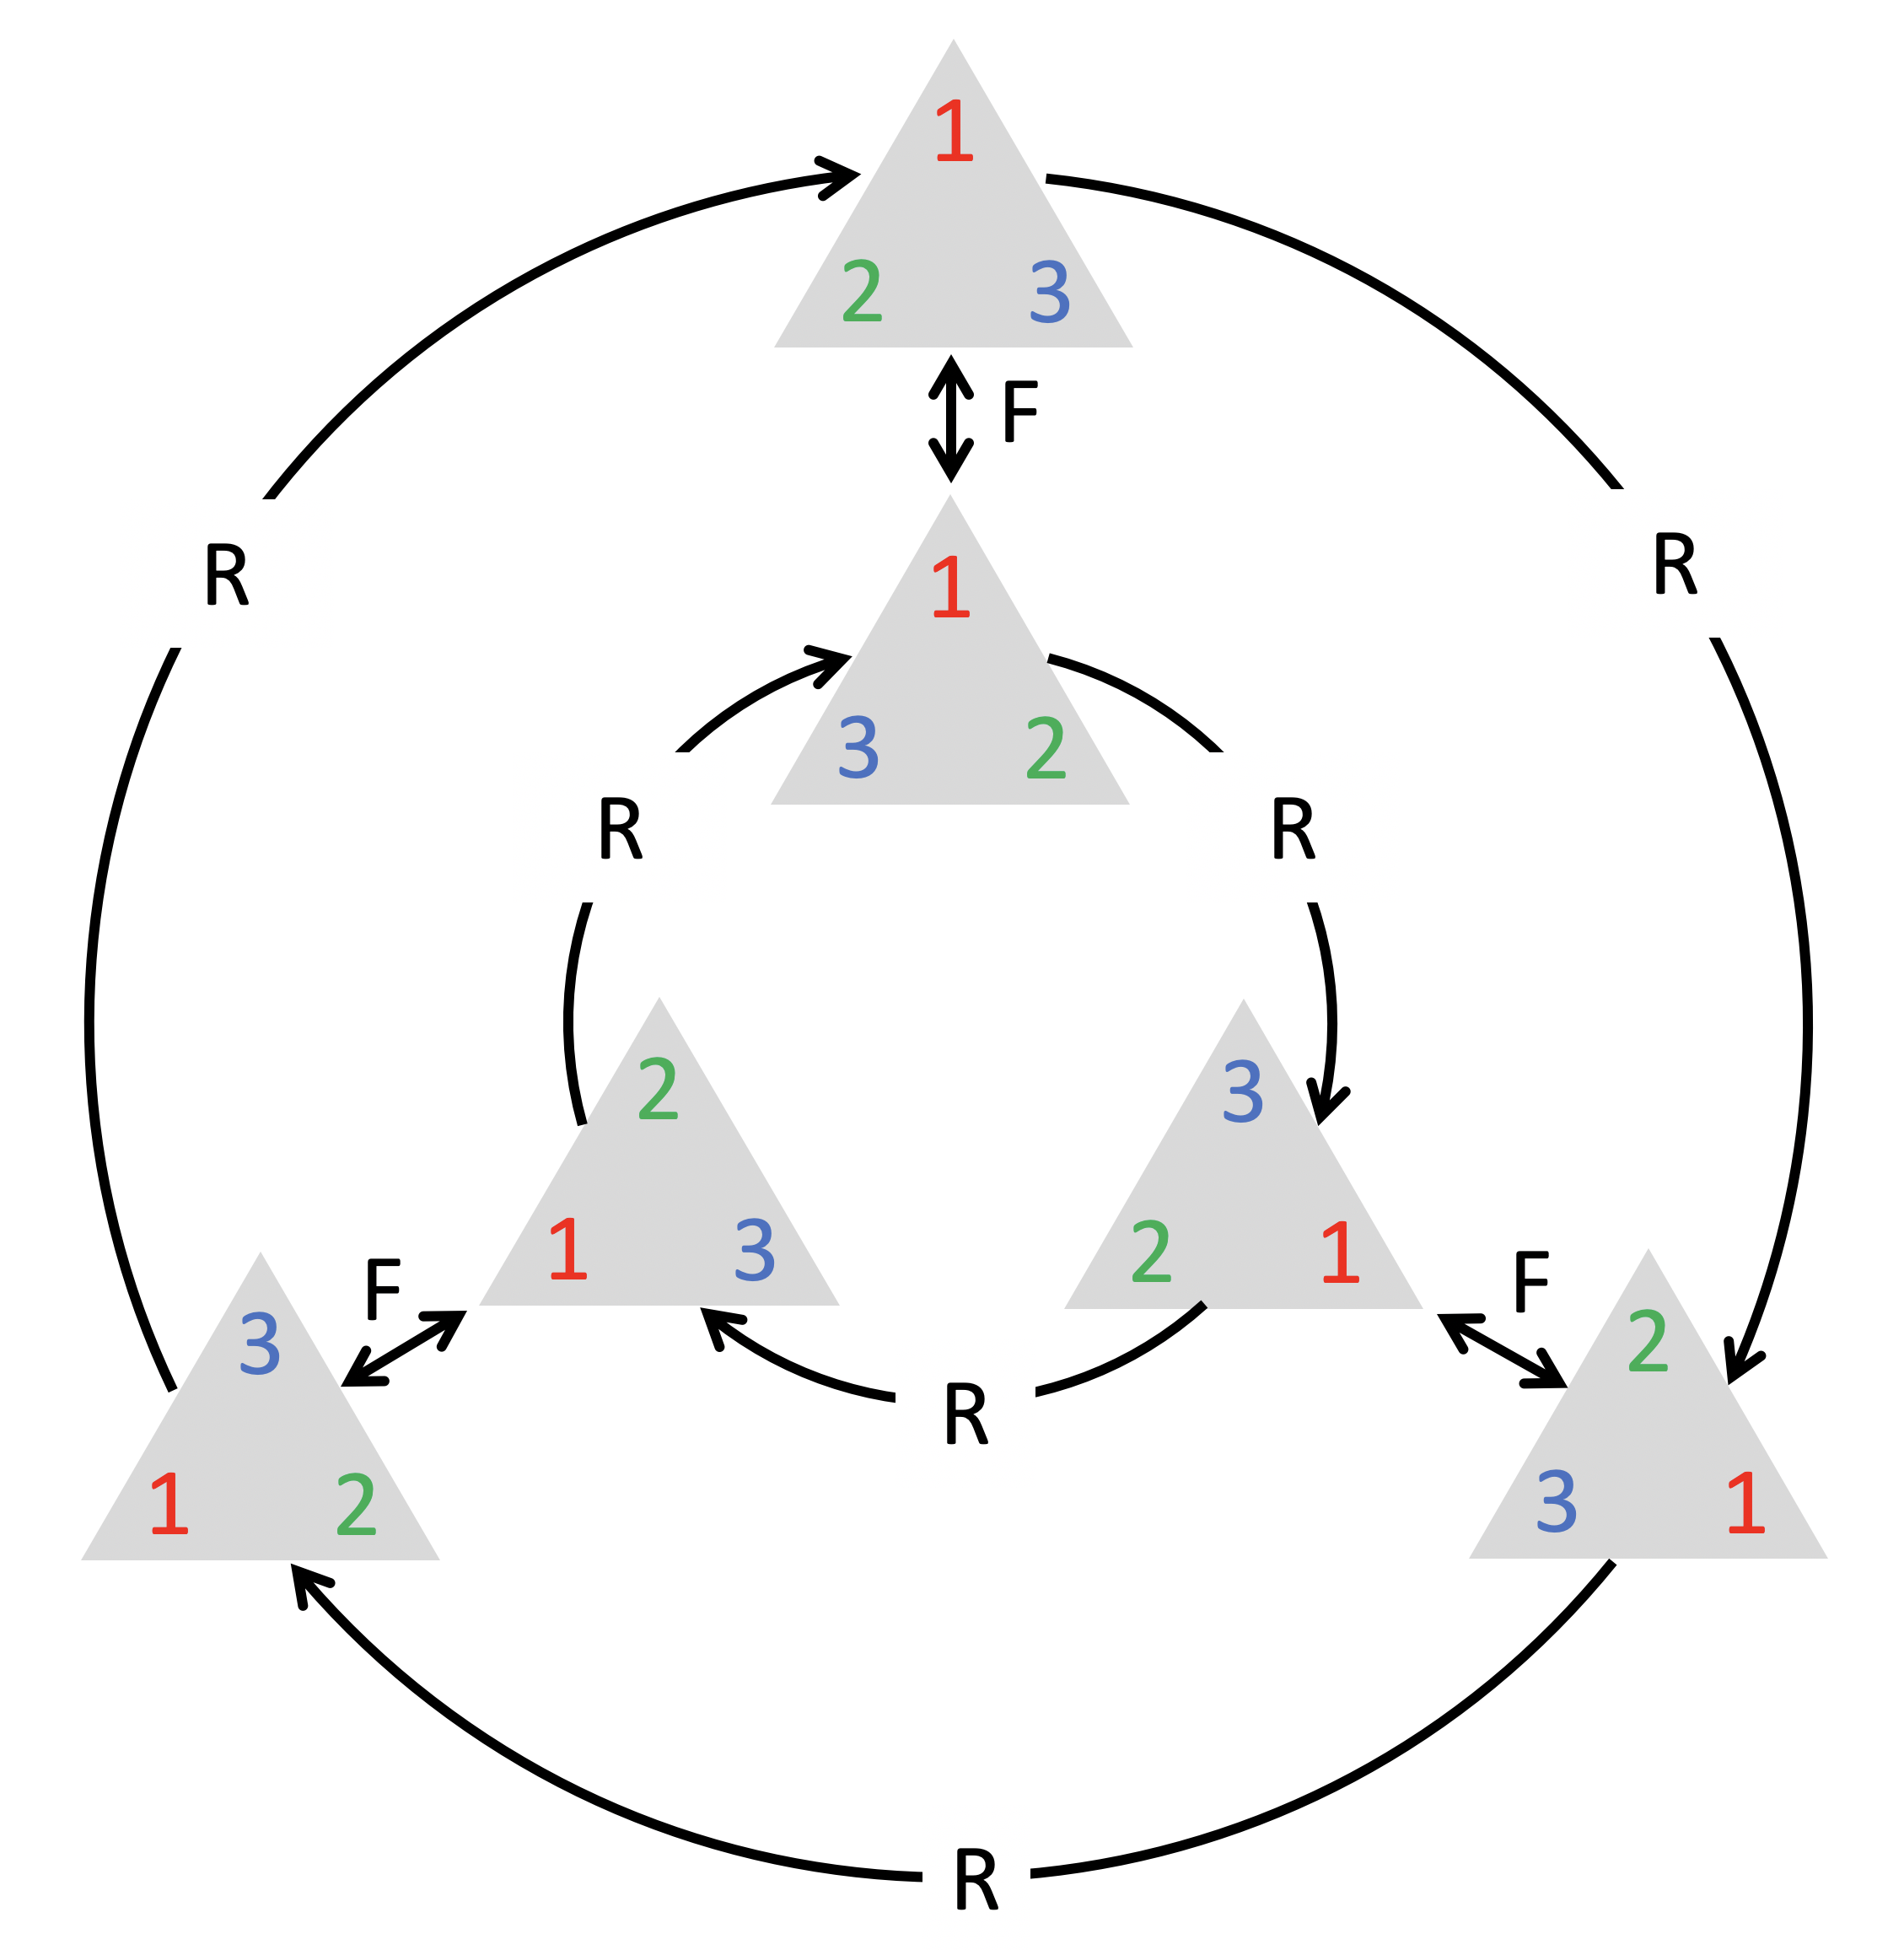
\includegraphics[width=0.45\linewidth]{figures/group_d3.png}
}
    \hspace{2mm}
    \raisebox{-0.5\height}{
        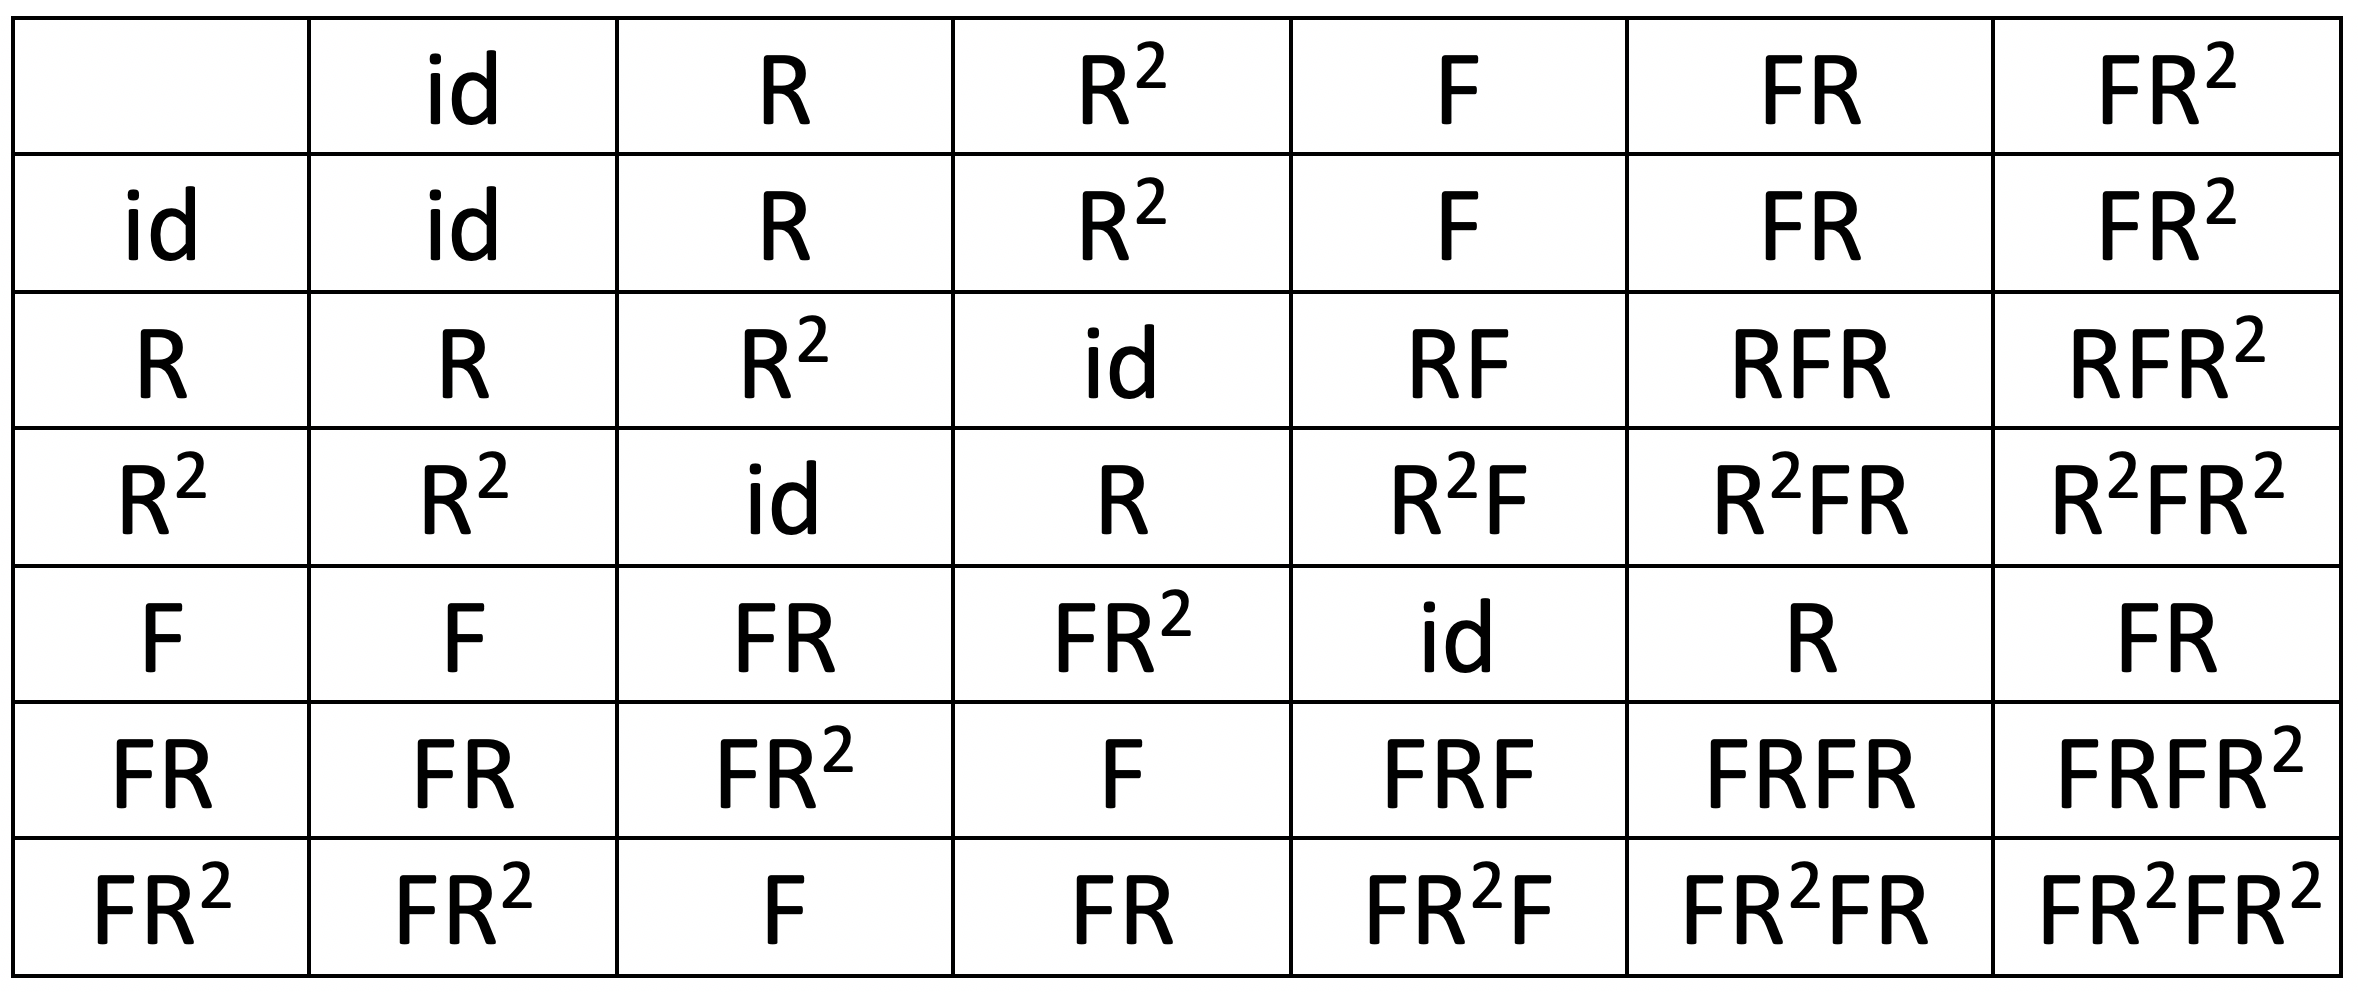
\includegraphics[width=0.48\linewidth]{figures/group_d3_m.png}
        }
%    \taco{TODO: figure of a triangle with labelled corners (0,1,2), and all permutations of it, as a Cayley diagram. Could add multiplication table of the group as well.}
    \caption{左：顶点标记为 $1, 2, 3$ 的等边三角形，以及该三角形所有可能的旋转与反射。三角形的旋转/反射对称群 $\mathrm{D}_3$ 仅由两个元素生成（旋转 $60^\circ$ 的 R 和反射 F），并且与三个元素的置换群 $\Sigma_3$ 相同。
    右：群 $\mathrm{D}_3$ 的乘法表。第 $\fg$ 行、第 $\fh$ 列的元素对应元素 $\fg \fh$。%\taco{\bf TODO: We need to reverse the Rotation arrows on the outer (or inner) ring. All rotations should be either clockwise or counter-clockwise}}
    \label{fig:group-example-d3-s3}
    }
\end{figure}

% Note that this definition provides a self-consistent description of a standalone object that is the main focus of study in group theory. Despite its apparent simplicity, this theory is rich with many deep results. 
% %despite the apparent simplicity of its basic definition.
% %
% %
% In geometry, key insights are obtained when transformations on a domain are modelled as elements of a group and the group theory formalism is used to study their properties --- this was exactly the breakthrough idea of Klein we have mentioned in the beginning of our discussion. 
% %
% %The way in which elements of symmetry groups act on points on a domain provides important insights about the structure of such domain --- 
% %
% %Group theory is a very rich area with many deep results, despite the apparent simplicity of its basic definition. 
% %
% %symmetry groups turn out to have rich internal algebraic structure with fascinating mathematical properties. 

\paragraph{群作用与群表示}
%
与其把群视为抽象实体，
我们更关心群如何\emph{作用}于数据。
%The structure of such groups reveals the symmetry concealed in the data, which in turn leads to powerful geometric priors. 
%
%The assumption In geometric deep learning, one typically starts 
由于我们假设数据以某个域 $\Omega$ 为基础，因此将研究群如何作用于 $\Omega$
（例如平面上点的平移），并由此得到同一个群在信号空间 $\mathcal{X}(\Omega)$ 上的作用
%\marginnote{Whenever possible, we will omit the range $\mathcal{C}$ for brevity.} %in which our data lives 
（例如平面图像与特征图的平移）。


% Taco: I am commenting this here, because 1) I think the notion of automorphism should be introduced differently. An auto is an iso from an object to itself. The meaning of iso depends on the context (category), i.e. on what properties/structure we wish to preserve. So when we introduce autos and subgroups, we should just say that we can preserve more or less structure, and get smaller or larger groups. 2) I think here the flow is disrupted a bit, and it would fit better in the deformation section.

% First, let us consider a broad class of bijective domain transformations called {\em automorphisms}
% $$\mathrm{Aut}(\Omega) = \{ \tau: \Omega \xrightarrow{1:1} \Omega \}.$$ 
% %
% Automorphisms also form a group with the composition operation. 
% %
% We can consider symmetries as `subsets' of automorphisms that preserve some structure: for example, in the plane the {\em Euclidean group} $\mathrm{E}(2)$ is the group of transformations of $\R^2$ that preserves Euclidean distances\marginnote{Distance-preserving transformations are called {\em isometries}. According to Klein's Erlangen Programme, the classical Euclidean geometry arises from this group.}, and consists of translations, rotations, and reflections.
% %
% More formally, a symmetry group $\fG$ constitutes a {\em subgroup} of the automorphism group $\mathrm{Aut}(\Omega)$: 

% \begin{tcolorbox}[width=\linewidth,
%                   boxsep=0pt,
%                   left=7.5pt,
%                   right=7.5pt,
%                   top=7.5pt,
%                   bottom=7.5pt,
%                   arc=0pt,
%                   boxrule=0pt,toprule=0pt,
%                   colback=boxgray,
%                   ]%%
% Let $(\fG,\circ)$ be a group and $\mathfrak{H} \subseteq \fG$ a subset. $\mathfrak{H}$ is said to be a {\em subgroup} of $\fG$ if $(\mathfrak{H},\circ)$ constitutes a group with the same operation. 
% \end{tcolorbox}


%we have considered so far are subgroups of $\mathrm{Aut}(\Omega)$. \marginnote{A subset $\fG \subseteq \frak{H}$ is said to be a {\em subgroup} of a group $(\frak{H}, \circ)$ if it forms a group $(\frak{G}, \circ)$ with the same operation.}



%\michael{do we use the . notation? $\fg.u$ of $\fg u$ but $\fg.x$}

群 $\fG$ 在集合 $\Omega$ 上的\emph{群作用}\marginnote{严格来说，这里定义的是{\em 左}群作用。}
%If $\fG$ is a group of transformations acting on elements of $\Omega$, a \emph{group action}\marginnote{Technically, what we define here is a {\em left} group action, since groups in general are non-commutative. } 
定义为映射 $(\fg, u) \mapsto \fg.u$；它把群元素 $\fg \in \fG$ 和点 $u\in \Omega$ 与 $\Omega$ 上的另一个点联系起来，并且
%$(\fg, u) \mapsto \fg.u$
%$(g, x) \in \gG \times \gX \mapsto g.x \in \gX$, 
%that 
与群运算相容，即 $\fg.(\fh.u) = (\fg \fh).u$ 对所有 $\fg, \fh \in \fG$ 和 $u \in \Omega$ 都成立。
%
后续各节将看到大量群作用的实例。
%including translation groups acting on grids or permutation groups acting on sets and graphs.
% TODO: add definition block for group action?
%\michael{\bf [MB: is $g.x$ a standard notation? I suggest $\fg$ as notation for groups]}
%
%Most of the domains we will discuss in this book have some natural symmetries. 
例如，在平面上，{\em 欧氏群} $\mathrm{E}(2)$ 是保持 $\R^2$ 中欧氏距离的变换群\marginnote{保持距离的变换称为{\em 等距变换}。根据 Klein 的 Erlangen Programme，经典欧氏几何由该群产生。}，它由平移、旋转和反射组成。
%collection of translation, rotation, and reflection transformations preserving Euclidean distances, so this group acts naturally on the plane.
然而，同一个群也可以作用于平面上的\emph{图像}空间（通过平移、旋转和翻转像素网格），以及神经网络学习到的表示空间。
%
%
更准确地说，如果群 $\fG$ 作用于 $\Omega$，那么可以自动得到 $\fG$ 在空间 $\mathcal{X}(\Omega)$ 上的作用：
%\marginnote{When it is clear from the context, we shall simplify the notation and simply write $\mathcal{X}$ for such space.}
%\michael{Do we need to carry the C here? It is not used; we only need to say that X is a vector space. I suggest to simplify the notation as much as possible. }
\begin{equation}
    (\fg . x)(u) = x(\fg^{-1} u).
    \label{eq:group_action}
\end{equation}
由于 $\fg$ 上存在逆，这确实是一个有效的群作用，因为有 $(\fg . (\fh . x))(u) = ((\fg \fh) . x)(u)$。%(exercise).
%: $(\fg . (\fh . f))(x) = (\fh . f)(\fg^{-1} x) = f(\fh^{-1} \fg^{-1} x) = f((\fg \fh)^{-1} x) = ((\fg \fh). f)(x)$. % leave as exercise?
%\michael{Is this standard notation? Looks abusive to use . for action on $x$ and $u$.}

%
%In our context, the central importance of symmetry groups is due to the fact that they also interact nicely with other less-structured objects. If $\fG$ is a group of transformations acting on elements of some arbitrary set $\gX$, a \emph{group action} is defined as a mapping 
%$(\fg, x) \mapsto \fg.x$
%$(g, x) \in \gG \times \gX \mapsto g.x \in \gX$, 
%that is compatible with the group operations in the sense that $\fg.(\fh.x) = (\fg \circ \fh).x$ for all $\fg, \fh \in \fG$ and $x \in \gX$. We shall see numerous instances of group actions in the next chapters, including translation groups acting on grids or permutation groups acting on sets and graphs.
% TODO: add definition block for group action?
%\michael{\bf [MB: is $g.x$ a standard notation? I suggest $\fg$ as notation for groups]}

全文将反复遇到的最重要一类群作用是\emph{线性}群作用，也称为{\em 群表示}。
式~(\ref{eq:group_action}) 中信号上的作用确实是线性的，其含义是
$$
\fg . (\alpha x + \beta x') = \alpha (\fg . x) + \beta (\fg . x') $$
%
该等式对任意标量 $\alpha, \beta$ 和信号 $x, x' \in \mathcal{X}(\Omega)$ 都成立。
%
可以把线性作用描述为映射 $(\fg, x) \mapsto \fg.x$，且该映射关于 $x$ 线性；等价地，通过柯里化，
%\footnote{Currying is the technique of converting a function that takes multiple arguments into a sequence of functions that each take a single argument.}
也可以把它描述为映射 $\rho : \fG \rightarrow \R^{n \times n}$\marginnote{当 $\Omega$ 是无限集时，信号空间 $\mathcal{X}(\Omega)$ 是无限维的，此时 $\rho(\fg)$ 是该空间上的线性算子，而不是有限维矩阵。不过在实践中，总是必须将其离散化为有限网格。}，该映射为每个群元素 $\fg$ 指定一个（可逆）矩阵 $\rho(\fg)$。
%\michael{Do we want to say representation can be over different space, and here we are interested in the space of signals? We need to say this is a vector space. }
矩阵的维数 $n$ 通常是任意的，不一定与群的维数或 $\Omega$ 的维数相关；但在深度学习应用中，$n$ 通常是群所作用的特征空间维数。
例如，可以让二维平移群作用于具有 $n$ 个像素的图像空间。

%\michael{\bf [MB: $n$ has to be defined. This paragraph needs a bit more details/polishing]}
与一般群作用一样，为群元素指定矩阵的方式应与群作用相容。
更具体地说，表示复合群元素 $\fg \fh$ 的矩阵，应等于 $\fg$ 与 $\fh$ 的表示矩阵之积：
%\begin{equation}
%    \rho(\fg \fh) = \rho(\fg) \rho(\fh).
%\end{equation}
%\michael{Can we just call this associativity? } \taco{No; both the group operation $\fg \fh$ and the matrix product $\rho(\fg) \rho(\fh)$ are associative, but the equation here says that $\rho$ is a homomorphism. Associativity involves three things being multiplied, $a(bc) = (ab)c$, but here we have two group elements $\fg, \fh$ and one mapping $\rho$, so it's different.}

% History of symmetries in mathematics and physics:
% \begin{itemize}
%     \item Kepler laws of planetary motion. 
%     \item Lagrangian and Hamiltonian of Mechanics invariant to observer frame of reference. 
%     \item Relativity? 
%     \item In mathematics, example of Galois Theory to study the roots of polynomial equations. The structure of such roots is revealed by studying their symmetries. 
% \end{itemize}

\begin{tcolorbox}[width=\linewidth,
                  boxsep=0pt,
                  left=7.5pt,
                  right=7.5pt,
                  top=7.5pt,
                  bottom=7.5pt,
                  arc=0pt,
                  boxrule=0pt,toprule=0pt,
                  colback=boxgray,
                  ]%%
    $n$ 维实\emph{表示}是群 $\fG$ 上的映射 $\rho : \fG \rightarrow \R^{n \times n}$；它为每个 $\fg \in \fG$ 指定一个\emph{可逆}矩阵 $\rho(\fg)$，并满足条件 $\rho(\fg \fh) = \rho(\fg) \rho(\fh)$，且这一条件对所有 $\fg, \fh \in \fG$ 成立。
    \marginnote{类似地，复表示是满足同一等式的映射 $\rho : \fG \rightarrow \mathbb{C}^{n \times n}$。}
    如果矩阵 $\rho(\fg)$ 对所有 $\fg \in \fG$ 都是酉矩阵或正交矩阵，则称该表示为\emph{酉表示}或\emph{正交表示}。
\end{tcolorbox}

用群表示的语言表述，$\fG$ 在信号 $x \in \mathcal{X}(\Omega)$ 上的作用定义为 $\rho(\fg) x(u) = x(\fg^{-1} u)$。
%
再次验证可得
$$
(\rho(\fg) (\rho(\fh) x))(u) = (\rho(\fg \fh) x)(u).
$$
%



% Removing stuff on subgroups and homogeneous spaces, as we don't really need it to talk about groups, representations and equivariance.
% % Consider moving this right after the definition of group, since the notion of subgroup does not rely on the notion of group action... 
% A subset of a group that is itself a group (i.e. is closed under composition and inverses, and contains the identity) is called a \emph{subgroup}.
% For example, the group $\mathrm{E}(2)$ contains the subset of rotations and translations (also called `roto-translations'), which is closed under composition and forms a group called the {\em special Euclidean group} $\SE{2}$. Finally, translations by themselves form the {\em translation group}. 
% %


% The plane is an example of a space in which ``all points are the same'', in the sense that one point can be transformed into another by means of a symmetry. 
% %
% Such a space is said to be {\em homogeneous} and requires that for any two points $u, v \in \Omega$ there is $\fg \in \fG$ such that $u = \fg v$. 
% %or in other words, one point can be transformed into another by means of a symmetry. 


\begin{figure}
    \centering
    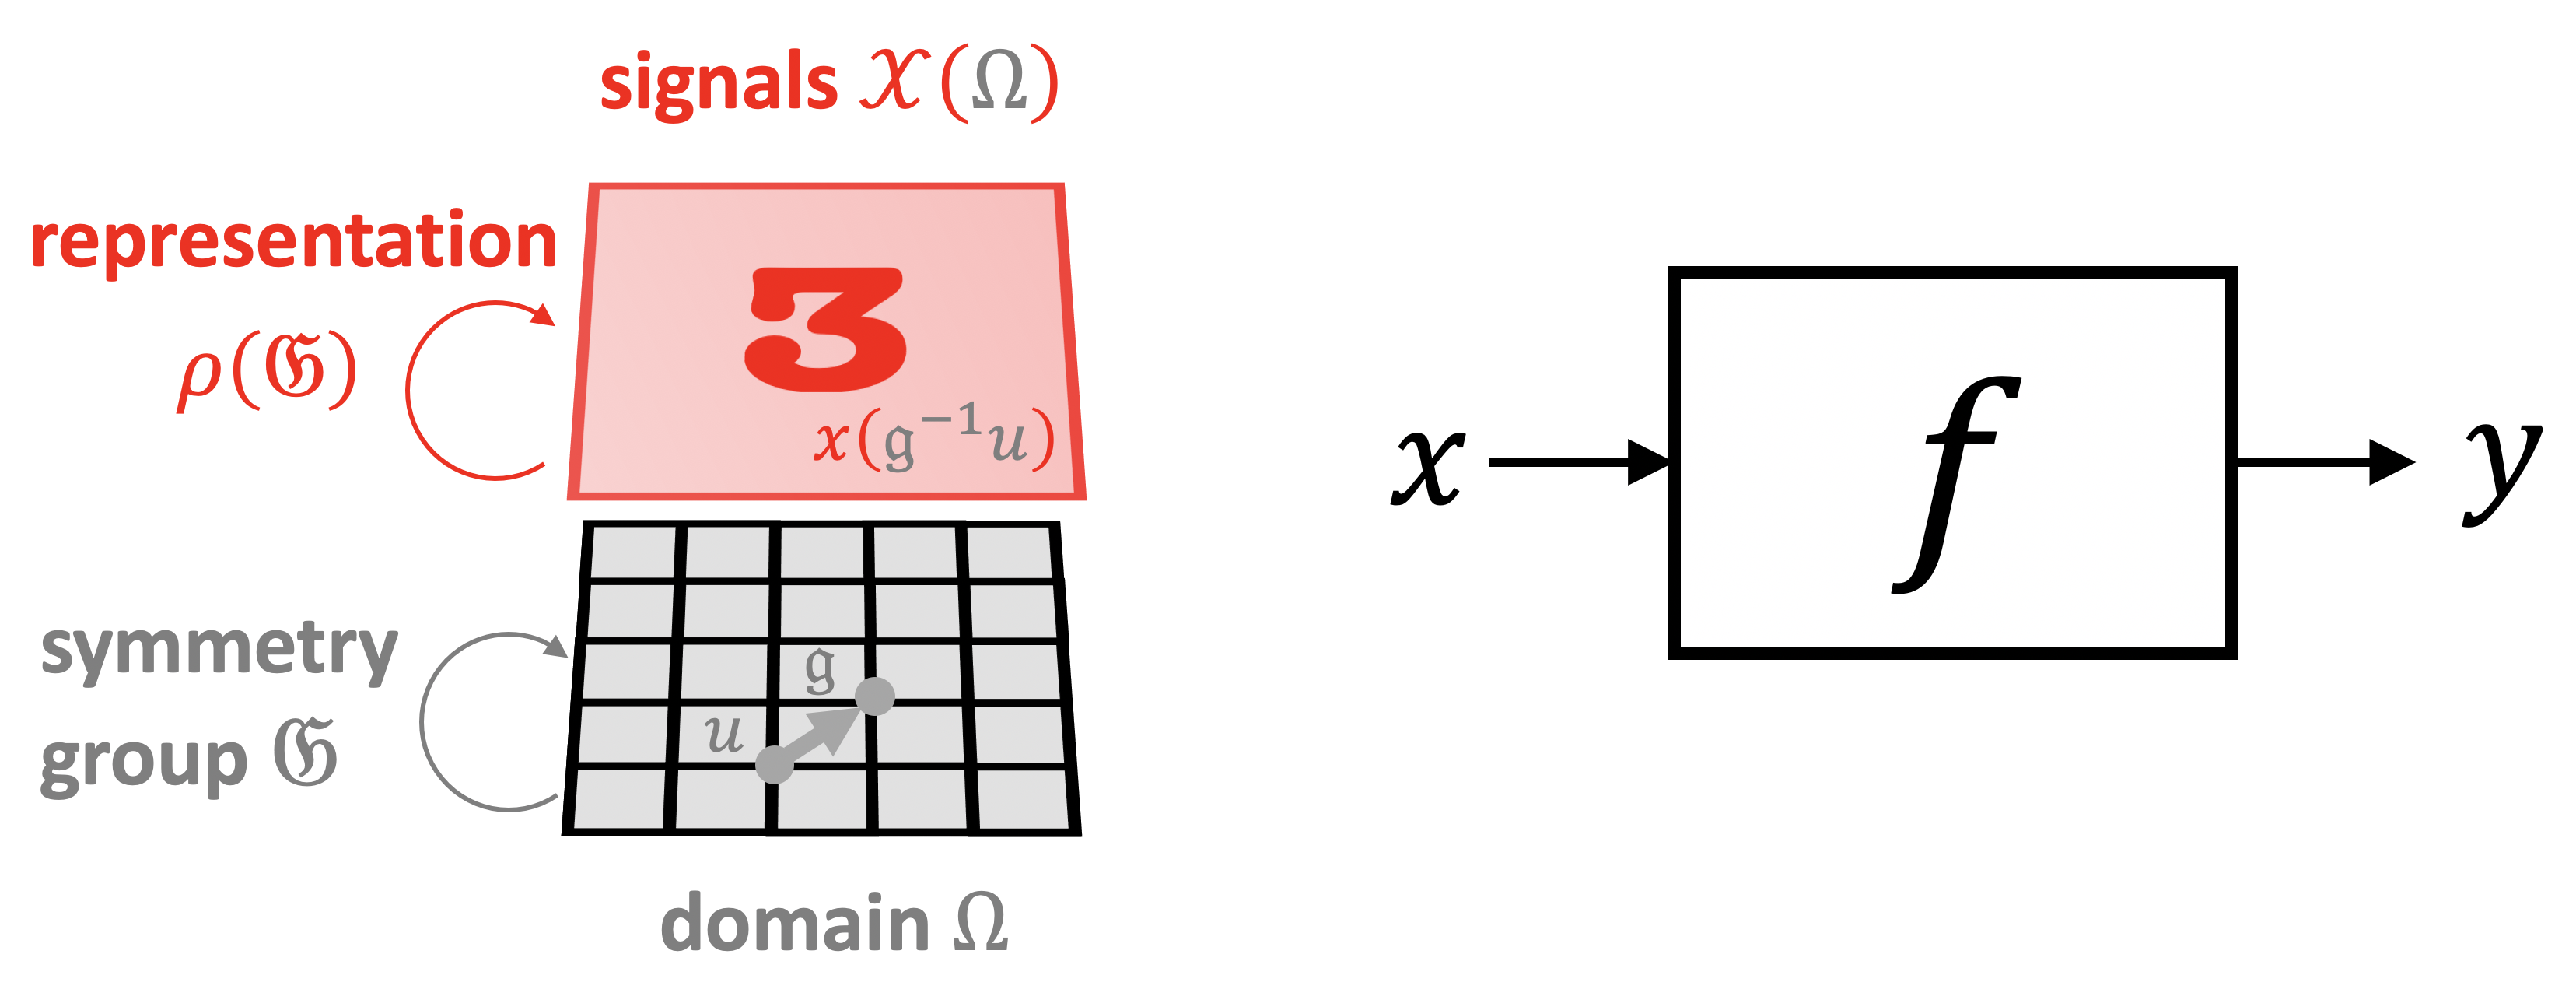
\includegraphics[width=0.75\linewidth]{figures/geom_prior.png}%groups1.pdf}
    \caption{
    几何深度学习所关注的三个空间：（物理）{\em 域} $\Omega$、{\em 信号}空间 $\mathcal{X}(\Omega)$，以及{\em 假设}类 $\mathcal{F}(\mathcal{X}(\Omega))$。
    %
    域 $\Omega$ 的对称性（由群 $\fG$ 刻画）作用于信号 $x\in \mathcal{X}(\Omega)$，这一作用由群表示 $\rho(\fg)$ 实现，从而对作用于这类信号的函数 $f\in \mathcal{F}(\mathcal{X}(\Omega))$ 施加结构。
    }
    \label{fig:symmetryactors}
\end{figure}


\paragraph{不变函数与等变函数}

域 $\Omega$ 是信号 $\mathcal{X}(\Omega)$ 的底层域；它所具有的对称性，会对定义在这类信号上的函数 $f$ 施加结构。
%
事实证明，这是一种强有力的归纳偏置；它提高学习\marginnote{一般而言，$f$ 同时依赖于信号和域，即 $\mathcal{F}(\mathcal{X}(\Omega), \Omega)$。为简洁起见，我们通常省略后一种依赖。}效率，方式是把可能插值函数的空间 $\mathcal{F}(\mathcal{X}(\Omega))$ 缩减为满足对称性先验的函数。
%
%Adding such known symmetries into the function hypothesis class of a machine learning system is a powerful inductive bias, improving learning efficiency by reducing the space of possible interpolants to those which satisfy the symmetry priors. 
%
本文将研究的两个重要情形是{\em 不变}函数与{\em 等变}函数。


%is its output is unaffected by the action of the group on the argument


\begin{tcolorbox}[width=\linewidth,
                  boxsep=0pt,
                  left=7.5pt,
                  right=7.5pt,
                  top=7.5pt,
                  bottom=7.5pt,
                  arc=0pt,
                  boxrule=0pt,toprule=0pt,
                  colback=boxgray,
                  ]%%
    函数 $f: \mathcal{X}(\Omega) \rightarrow \mathcal{Y}$ 是 $\fG$-{\em 不变的}，如果
    $
    f(\rho(\fg)x) = f(x)$ 对所有 $\fg \in \fG$ 和 $x \in \mathcal{X}(\Omega)$ 都成立；也就是说，其输出不受输入上群作用的影响。
\end{tcolorbox}


不变性的一个经典例子是{\em 平移不变性}，\marginnote{注意，信号处理书籍通常使用“平移不变性”一词来指平移等变性，例如线性平移不变系统。}
它出现在图像分类等计算机视觉与模式识别应用中。此时函数 $f$（通常实现为卷积神经网络）输入一幅图像，并输出该图像包含某个类别对象（例如猫或狗）的概率。%
%
通常可以合理假设，分类结果不应受到对象在图像中位置的影响，即函数 $f$ 必须具有平移不变性。
%
多层感知机虽然能够逼近任何光滑函数，却不具备这一性质；这是二十世纪七十年代将这类架构应用于模式识别问题的早期尝试失败的原因之一。
%
以卷积神经网络为典型代表的局部权重共享神经网络架构，其发展动力之一正是实现平移不变的物体分类。


然而，如果更仔细地考察 CNN 的卷积层，就会发现它们并非平移不变，而是{\em 平移等变的}：换言之，将卷积层的输入平移一定距离，会使输出特征图平移相同距离。

\begin{tcolorbox}[width=\linewidth,
                  boxsep=0pt,
                  left=7.5pt,
                  right=7.5pt,
                  top=7.5pt,
                  bottom=7.5pt,
                  arc=0pt,
                  boxrule=0pt,toprule=0pt,
                  colback=boxgray,
                  ]%%
    函数 $f: \mathcal{X}(\Omega) \rightarrow \mathcal{X}(\Omega)$ 是 $\fG$-{\em 等变的}，如果\marginnote{
    更一般地，可能有 $f: \mathcal{X}(\Omega) \rightarrow \mathcal{X}(\Omega')$，其中输入与输出空间具有不同的域 $\Omega, \Omega'$ 和表示 $\rho$、$\rho'$，而这些表示属于同一个群 $\fG$。
    在这种情况下，等变性定义为 $f(\rho(\fg)x) = \rho'(\fg) f(x)$。
    %symmetry groups, $\fG$ and $\fG'$. In this case, equivariance is defined as $ f(\rho(\fg)x) = \rho'(\fg) f(x)$, where $\rho'$ is the representation of $\fG'$.
    } 
    $f(\rho(\fg)x) = \rho(\fg) f(x)$ 对所有 $\fg \in \fG$ 都成立；也就是说，输入上的群作用以相同方式影响输出。
\end{tcolorbox}




再次以计算机视觉为例，需要平移等变性的典型应用是图像分割，其中 $f$ 的输出是逐像素图像掩码。
%
显然，分割掩码必须随输入图像的平移而移动。
在本例中，输入域与输出域相同；但由于输入有三个颜色通道，而输出对每个类别有一个通道，因此表示 $(\rho, \mathcal{X}(\Omega, \mathcal{C}))$ 与 $(\rho', \mathcal{X}(\Omega, \mathcal{C}'))$ 略有不同。


不过，即使是前述图像分类用例，通常也是由一系列卷积（平移等变）层实现，随后接全局池化（平移不变）。
%
正如第~\ref{sec:gdl_blueprint} 节将看到的，这是包括 CNN 和图神经网络（GNN）在内的大多数深度学习架构的一般蓝图。
%: a sequence of equivariant layers, optionally followed by invariant layers. 


%In supervised learning, the goal is to approximate some function $f : \mathcal{X} \rightarrow \mathcal{X}'$ from a finite set of samples.
%In many cases, the problem has symmetries, which means that $f$ is either invariant ($f(\rho(\fg) x) = f(x)$ for all $\fg \in \fG$) or equivariant ($f(\rho(\fg) x) = \rho'(\fg) f(x)$).
%For instance, in image classification the class label is invariant, whereas the segmentation mask is equivariant. 
% In machine learning, where one tries to approximate some unknown function $f$ from a finite set of samples, $f$ often has known symmetries.
% Canonical examples include translations in computer vision and image classification tasks, rotations in molecular prediction problems, or permutations in 3D graphics point-cloud processing tasks. 
% %
% In such settings, given some domain $\gX$ with a certain symmetry group $\fG$, we say that 
% $f: \gX \to \gY$ is $\fG$\emph{-invariant} if $f(\fg.x) = f(x)$ for all $x\in \gX$ and $\fg \in \fG$. If in addition $\fG$ is also acting on $\gY$, we say that $f$ is $\fG$\emph{-equivariant} if $f(\fg.x) = \fg.(f(x))$.
% % We will explore these concepts in detail in Chapter ??. 
%Adding such known symmetries into the function hypothesis class %$\gF$ 
%of a machine learning system is a powerful inductive bias, improving learning efficiency by reducing the space of possible interpolants to those which satisfy the symmetry priors. 


% Possible todo's for this section:
% Explain in/equivariance mathematically (at a high level only)
% Explain group representations (idem)


%\taco{TODO: add definition of space of signals, and regular rep acting on it}

%\taco{TODO: Figure showing domain Omega, group action of G on Omega, and the space of functions X on Omega}

\subsection{同构与自同构}
\label{sec:isomorphism}

\paragraph{子群与结构层次}

如前所述，对称性\marginnote{不同对象之间保持结构的可逆映射通常统称为{\em 同构}（希腊语意为“形状相同”）。对象到自身的同构称为{\em 自同构}，即对称性。}
%We will mainly use this term for maps preserving the connectivity of graphs.}
是保持某种性质或结构的变换；对于给定结构，所有这类变换的集合构成一个对称群。
我们关注的结构往往不止一种，因此可以在域 $\Omega$ 上考虑若干{\em 结构层次}。
%
%We can thus formalise symmetries as invertible maps $\tau: \Omega \rightarrow \Omega$ that preserve some structure. % and satisfy the group axioms with the function composition operation.  
因此，何种变换算作对称性取决于所考虑的结构；但在所有情况下，对称性都是尊重该结构的可逆映射。

在最基本的层次上，域 $\Omega$ 是一个\emph{集合}，所含结构最少：只能说该集合具有某个\emph{基数}\marginnote{对于有限集，基数是集合中的元素数量（“大小”）；对于无限集，基数表示不同类型的无穷，例如自然数的可数无穷，或连续统 $\R$ 的不可数无穷。}。%, and which elements are members of the set.
保持这种结构的自映射是\emph{双射}（可逆映射），可以将其视为集合层次的对称性。
%A more formal way to say the same is that the automorphism group $\mathrm{Aut}(\Omega)$ in the category of sets is the group of bijections $\tau : \Omega \rightarrow \Omega$.
%Such maps are often referred to as (set-){\em automorphisms} and denoted by $\mathrm{Aut}(\Omega)$. 
%
通过检查公理可以容易地验证这构成一个群：两个双射的复合仍是双射（封闭性）；结合律来自函数复合的结合律；映射 $\tau(u)=u$ 是单位元；并且按定义，每个 $\tau$ 都存在逆，满足 $(\tau \circ \tau^{-1})(u) = (\tau^{-1} \circ \tau)(u) =u$。


根据具体应用，还可能存在更高的结构层次。
%
例如，如果 $\Omega$ 是拓扑空间，可以考虑保持{\em 连续性}的映射：这类映射称为{\em 同胚}；除去集合之间双射这一要求外，它们自身连续，逆映射也连续。
%
直观地说，连续函数具有良好性质，它把点 $u$ 周围某邻域（开集）中的点映射到 $\tau(u)$ 周围的一个邻域中。
%Thus, homeomorphisms $\tau : \Omega \rightarrow \Omega$ are the automorphisms / symmetries of $\Omega$ viewed as a topological space.


%
%
还可以进一步要求映射及其逆都是（连续）{\em 可微的}，\marginnote{每个可微函数都是连续的。如果映射“足够多次”连续可微，则称其为{\em 光滑的}。}即映射及其逆在每一点都有导数（且导数也连续）。
%
这需要可微流形所具有的进一步可微结构；在这种结构下，这类映射称为{\em 微分同胚}，记为 $\mathrm{Diff}(\Omega)$。
%These are the automorphisms of smooth manifolds.
%
%
后文还会遇到其他结构，例如{\em 距离}或{\em 度量}（保持它们的映射称为{\em 等距变换}），以及{\em 取向}（据我们所知，保持取向的映射没有通用的希腊语名称）。


\begin{tcolorbox}[width=\linewidth,
                  boxsep=0pt,
                  left=7.5pt,
                  right=7.5pt,
                  top=7.5pt,
                  bottom=7.5pt,
                  arc=0pt,
                  boxrule=0pt,toprule=0pt,
                  colback=boxgray,
                  ]%%
{\em 度量}或{\em 距离}是函数 $d:\Omega\times\Omega \rightarrow [0,\infty)$，并对所有 $u,v,w \in \Omega$ 满足：\vspace{3mm}\\
%\begin{enumerate}
    %\item 
    \noindent {\em 	同一性：} $d(u,v) =0$ 当且仅当 $u=v$。\vspace{2mm}\\
    \noindent  {\em 对称性：} $d(u,v) = d(v,u)$。\vspace{2mm}\\
    \noindent  {\em 三角不等式：} $d(u,v) \leq  d(u,w) + d(w,v)$。\vspace{2mm}\\
%\end{enumerate}

配备度量的空间 $(\Omega,d)$ 称为{\em 度量空间}。

\end{tcolorbox}




%an image plane can be viewed as a smooth manifold, in which case any smooth deformation (diffeomorphism) should be considered a symmetry.
%In practice the object identity will not be preserved by arbitrarily large deformations, so we may add a distance metric, i.e. view the image plane as a Riemannian manifold, in which case only distance-preserving transformations (isometries) can be considered as symmetries.
%As a further example, independently of whether we care about distances, we can assign an \emph{orientation} to the plane, i.e. clockwise or counterclockwise, and consider only orientation-preserving transformations.

应当考虑何种结构层次取决于具体问题。
例如，在分割组织病理学切片图像时，我们可能希望把图像的翻转版本视为等价（因为样本放到显微镜下时可以翻转）；但在对道路标志分类时，则只希望把保持取向的变换视为对称性（因为反射可能改变标志的含义）。
%{\bf [Figure?]}

随着需要保持的结构层次增加，对称群会变小。
事实上，增加结构等价于选择一个\emph{子群}；子群是较大群的一个子集，其自身满足群公理：
%(i.e. it is closed under composition and inverses, and contains the identity).
 
 \begin{tcolorbox}[width=\linewidth,
                   boxsep=0pt,
                   left=7.5pt,
                   right=7.5pt,
                   top=7.5pt,
                   bottom=7.5pt,
                   arc=0pt,
                   boxrule=0pt,toprule=0pt,
                   colback=boxgray,
                   ]%%
 设 $(\fG,\circ)$ 为一个群，$\mathfrak{H} \subseteq \fG$ 为一个子集。称 $\mathfrak{H}$ 是 $\fG$ 的{\em 子群}，如果 $(\mathfrak{H},\circ)$ 在同一运算下构成群。
 \end{tcolorbox}
 
例如，欧氏等距变换群 $\E{2}$ 是平面微分同胚群 $\diff{2}$ 的子群，而保持取向的等距变换群 $\SE{2}$ 又是 $\E{2}$ 的子群。
这一结构层次遵循前言所述的 Erlangen Programme 思想：在 Klein 的构造中，射影几何、仿射几何与欧氏几何具有逐渐增多的不变量，并对应于逐渐缩小的群。


\paragraph{同构与自同构}
% Optional: discuss the notion of isomorphic objects, and present symmetries as self-isomorphisms i.e. automorphisms. Thus the notion of symmetry depends on the notion of iso, i.e. the category we're working in, i.e. the level of structure as discussed above.

我们已经把对称性描述为\emph{从对象到其自身}的、保持结构的可逆映射。
这类映射也称为\emph{自同构}，描述对象与其自身等价的一种方式。
然而，还有一类同样重要的映射称为\emph{同构}，用于表明两个不同对象之间的等价性。
这些概念经常被混淆，但为了使后续讨论清晰，有必要将其区分开来。

为理解二者的区别，考虑集合 $\Omega = \{0,1,2\}$。
集合 $\Omega$ 的自同构是双射 $\tau : \Omega \rightarrow \Omega$，例如循环移位 $\tau(u) = u + 1 \mod 3$。
这种映射保持基数性质，并把 $\Omega$ 映射到自身。
如果另有一个元素数量相同的集合 $\Omega' = \{a, b, c\}$，那么双射 $\eta : \Omega \rightarrow \Omega'$，例如 $\eta(0) = a$、$\eta(1) = b$、$\eta(2) = c$，就是一个{\em 集合同构}。

正如第~\ref{sec:proto-graphs} 节将针对图说明的，%$\Omega$,
结构的概念不仅包括节点数量，也包括连通性。
因此，同构 $\eta: \mathcal{V} \rightarrow \mathcal{V}'$ 位于两个图 $\mathcal{G}=(\mathcal{V},\mathcal{E})$ 与 $\mathcal{G}'=(\mathcal{V}',\mathcal{E}')$ 之间，是节点之间的双射；它把相连节点对映射为相连节点对，也把不相连节点对映射为不相连节点对。\marginnote{即 $(\eta(u),\eta(v)) \in \mathcal{V}'$ 当且仅当 $(u,v) \in \mathcal{V}$。}因此，两个同构图在结构上完全相同，区别仅在于节点次序。\marginnote{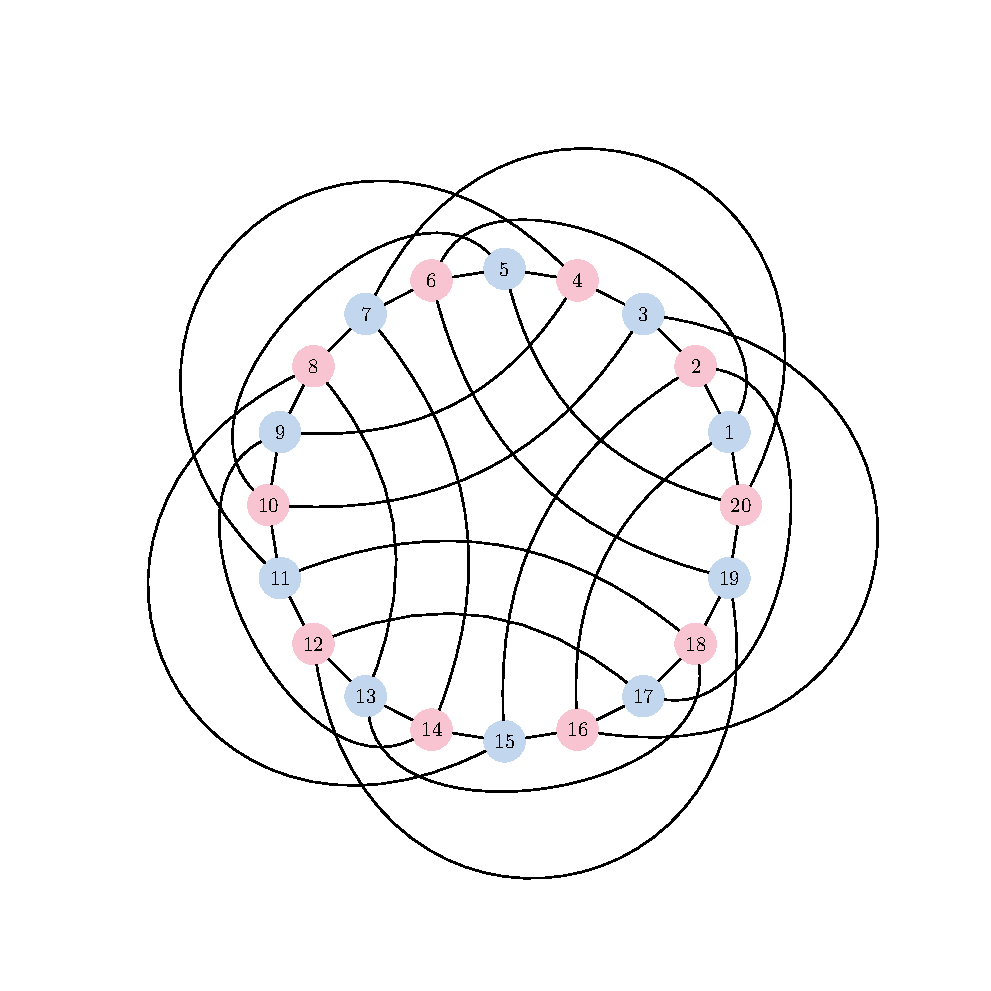
\includegraphics[width=\linewidth]{figures/folkman_g.pdf}\vspace{-2mm}\\ \emph{Folkman graph} \citep{folkman1967regular} 是一个具有 3840 个自同构的优美图实例，这一点可由绘制它的多种对称方式体现。}
%
另一方面，图的自同构或对称性是映射 $\tau : \mathcal{V} \rightarrow \mathcal{V}$；它在保持连通性的同时，把图的节点映射回自身。具有非平凡自同构（即 $\tau \neq \mathrm{id}$）的图呈现出对称性。
%\michael{Show in a figure}

%An isomorphism of graphs is thus not the same as a symmetry, but it is just as important that our neural network treat isomorphic objects equivalently.
% when we're dealing with isos vs autos. Example of sphere and graph

% same number of isos A -> B and autos A -> A. Isomorphic objects have isomorphic automorphism groups




\subsection{形变稳定性}
\label{sec:geom_stab}
%While the Fourier representation is useful to represent {\em signals} $\gX(\Omega)$ on a domain $\Omega$, it is not necessarily useful to regularise the space of {\em functions on such signals}, $\mathcal{F}(\mathcal{X}(\Omega))$ used in supervised learning problems. 
%
%Despite its far-reaching implications, the Fourier representation $\hat{x}$ is not necessarily useful to regularise the space of functions $\{ f : \gX \to \gY \}$, 
%the ultimate goal of supervised learning. 
%
第~\ref{sec:symmetries}--\ref{sec:isomorphism} 节引入的对称性形式体系刻画了一个理想化世界：我们确切知道哪些变换应被视为对称性，并希望{\em 精确地}尊重这些对称性。
%the transformations affecting the input are captured with simple mathematical models.
例如，在计算机视觉中，可以假设平面平移是精确对称性。
%model for input variability parametrised by only two degrees of freedom (the translations in the plane). 
然而，现实世界含有噪声，这种模型在两个方面存在不足。%: it only describes \emph{global} transformations, and

\marginnote{
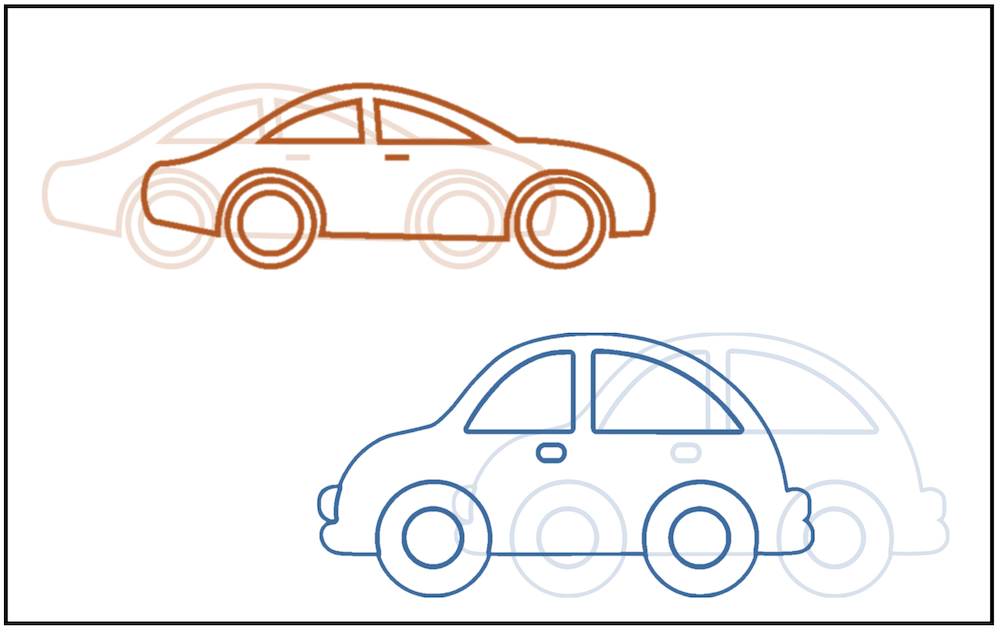
\includegraphics[width=0.95\linewidth]{figures/videosketch.png}
视频中以不同速度运动的两个对象定义了
平移群之外的变换。
}
首先，尽管这些简单群提供了理解域 $\Omega$ 的\emph{全局}对称性（进而理解其上信号 $\gX(\Omega)$ 的全局对称性）的方法，却不能很好地刻画\emph{局部}对称性。
%
例如，考虑一个视频场景%$x=x_t$
，其中有若干对象，每个对象都沿各自不同的方向运动。
在后续帧中，所得场景
%$x_{t+\delta t}$ 
将包含近似相同的语义信息，但没有任何全局平移能够解释一帧到另一帧的变换。
在其他情况下，例如摄像机观察到的可形变三维对象，要描述保持对象身份的变换群本身就非常困难。
这些例子说明，在现实中，我们更关心一个%beneath the global symmetry group lies a
大得多的变换集合，其中全局的精确不变性被局部的非精确不变性所取代。
%
在讨论中，我们将区分两种情形：一种是域 $\Omega$ 固定而信号 $x \in \gX(\Omega)$ 经历形变；另一种是域 $\Omega$ 本身可能发生形变。
%\taco{TODO: perhaps move this up, and discuss this as isomorphisms vs automorphisms?}

%In the language of group representations, we thus need to account for a broader class of bijective domain transformations called {\em automorphisms}, $\mathrm{Aut}(\Omega) = \{ \tau: \Omega \xrightarrow{1:1} \Omega \}$. 
\paragraph{对信号形变的稳定性}
在许多应用中，我们先验地知道，信号 $x$ 的小形变不应改变 $f(x)$ 的输出，因此很自然地会想把这类形变视为对称性。
例如，可以把小微分同胚 $\tau \in \diff{\Omega}$，甚至小双射，视为对称性。
然而，小形变可以复合成大形变，因此“小形变”不构成群\marginnote{例如，两个 $\epsilon$-等距变换的复合是一个 $2\epsilon$-等距变换，违反封闭性。}，也就不能只要求对小形变具有不变性或等变性。
由于大形变确实可能实质性改变输入的语义内容，因此把完整群 $\diff{\Omega}$ 用作对称群也并不可取。

更好的方法是，量化给定的 $\tau \in \diff{\Omega}$ 距给定对称子群 $\fG \subset \diff{\Omega}$（例如平移）有多“远”，所使用的复杂度度量为 $c(\tau)$，
并要求 $c(\tau) = 0$；每当 $\tau \in \fG$ 时，这一等式都成立。
这样，便可以用一种更“柔和”的\emph{形变稳定性}（或{\em 近似不变性}）概念，取代之前关于群作用下精确不变性与等变性的定义：
\begin{equation}
\label{eq:defstability1}
\| f(\rho(\tau) x) - f(x)\| \leq C c(\tau) \|x\|,~,~    \forall x\in \gX(\Omega)
\end{equation}
其中，与前面一样，$\rho(\tau)x(u) = x(\tau^{-1} u)$；$C$ 是与信号 $x$ 无关的某个常数。
满足上述等式的函数 $f\in \mathcal{F}(\mathcal{X}(\Omega))$ 称为{\em 几何稳定的}。
%
下一节~\ref{sec:scale_separation} 将给出这类函数的实例。


由于 $c(\tau)=0$ 对 $\tau \in \fG$ 成立，该定义推广了上文定义的 $\fG$-不变性性质。它在应用中的效用取决于是否引入适当的形变代价。对于定义在连续欧氏平面上的图像，
一种常见选择是 $c^2(\tau) := \int_\Omega \| \nabla \tau(u)\|^2 \mathrm{d}u$，它衡量 $\tau$ 的“弹性”，即它与常向量场位移之间的差异程度。
%
这种形变代价实际上是一个范数，通常称为{\em Dirichlet 能量}，可用于量化 $\tau$ 距平移群有多远。

%


% All of the symmetry groups we have considered and will consider in this book are subgroups of the group of bijections of $\Omega$.
% %The symmetry groups we have considered so far are subgroups of the group $\mathrm{Aut}(\Omega)$ of set-automorphisms of $\Omega$, or general domain transformations. 
% %
% For any such group $\fG$, 

% Same way as we had the symmetry group $\fG$ represented as a linear operator $\rho$ on $\mathcal{X}(\Omega)$, we can now do the same for $\mathrm{Aut}(\Omega)$ to lift diffeomorphisms of the domain into linear transformations on signals $x \in \gX(\Omega)$:
% %construct a linear operator $L_\tau: \gX(\Omega) \to \gX(\Omega)$ of the form 
% %that extend group actions, and which again lift into linear transformations , 
% $$
% (\rho(\tau) x)(u) = x( \tau^{-1}(u)). 
% $$  
% %$\rho(\fg), \fg \in \fG$, we thus need to consider linear transformations
% %
% This represents how the transformation of the domain $\Omega$ by an automorphism $\tau$ affects the signal $x \in \mathcal{X}(\Omega)$; see Figure \ref{fig:groupdeformation}. %
% Note that invariance to such large automorphism group is not a desired property, since large distortions of the domain 
% eventually destroy the semantic information of the input. 
% Instead, we can quantify how "far" a given $\tau \in \mathrm{Aut}(\Omega)$ is from a given symmetry subgroup $\fG \subset \mathrm{Aut}(\Omega)$ 
% with a complexity measure $c(\tau)$, so that $c(\tau) = 0$ whenever $\tau \in \fG$. 
% We can now replace our previous rigid definition of invariance and equivarance under group actions to a softer 
% \emph{deformation stability} principle:
% %Similarly to our definition of functions that are invariant and equivariant under group actions, 
% %we can have functions that are {\em approximately invariant} or {\em equivariant} under such automorphisms. 
% %
% %Such approximate invariance, to which we refer as {\em geometric stability}, can be expressed in the form of a bound %of the form
% \begin{equation}
% \label{eq:defstability1}
% \forall ~x\in \gX(\Omega)~,~\| f(\rho(\tau) x) - f(x)\| \leq C c(\tau) \|x\|,    
% \end{equation}
% with some constant $C$ independent of the signal $x$. A function $f\in \mathcal{F}(\mathcal{X}(\Omega))$ satisfying the above equation is said to be {\em geometrically stable}. 
% %
% Since $c(\tau)=0$ for $\tau \in \fG$, this definition generalises the $\fG$-invariance property defined above. Its utility in applications depends on introducing an appropriate deformation cost. In the case of images defined over a continuous Euclidean plane, 
% a relevant example is given by $c^2(\tau) := \int_\Omega \| \nabla \tau(u)\|^2 \mathrm{d}u$. This deformation cost is in fact a norm often called the {\em Dirichlet energy}, and used as a measure of elasticity of $\tau$. 
% %We will discuss these concepts in greater detail in Chapter ???.

% %To quantify this properly, we need some notion of metric or `distance' between maps and signals, as will be detailed in Section ??.  
% %
% %In some sense that will be formalized later, we expect our functions of interest to be \emph{almost} invariant/equivariant for transformations $L_\tau$ which are ``nearby" the group transformations $\rho(\fg)$ for $\fg \in \fG$.
% %We informally refer to this concept as \emph{geometric stability}. 

\begin{figure}[!htbp]
    \centering
    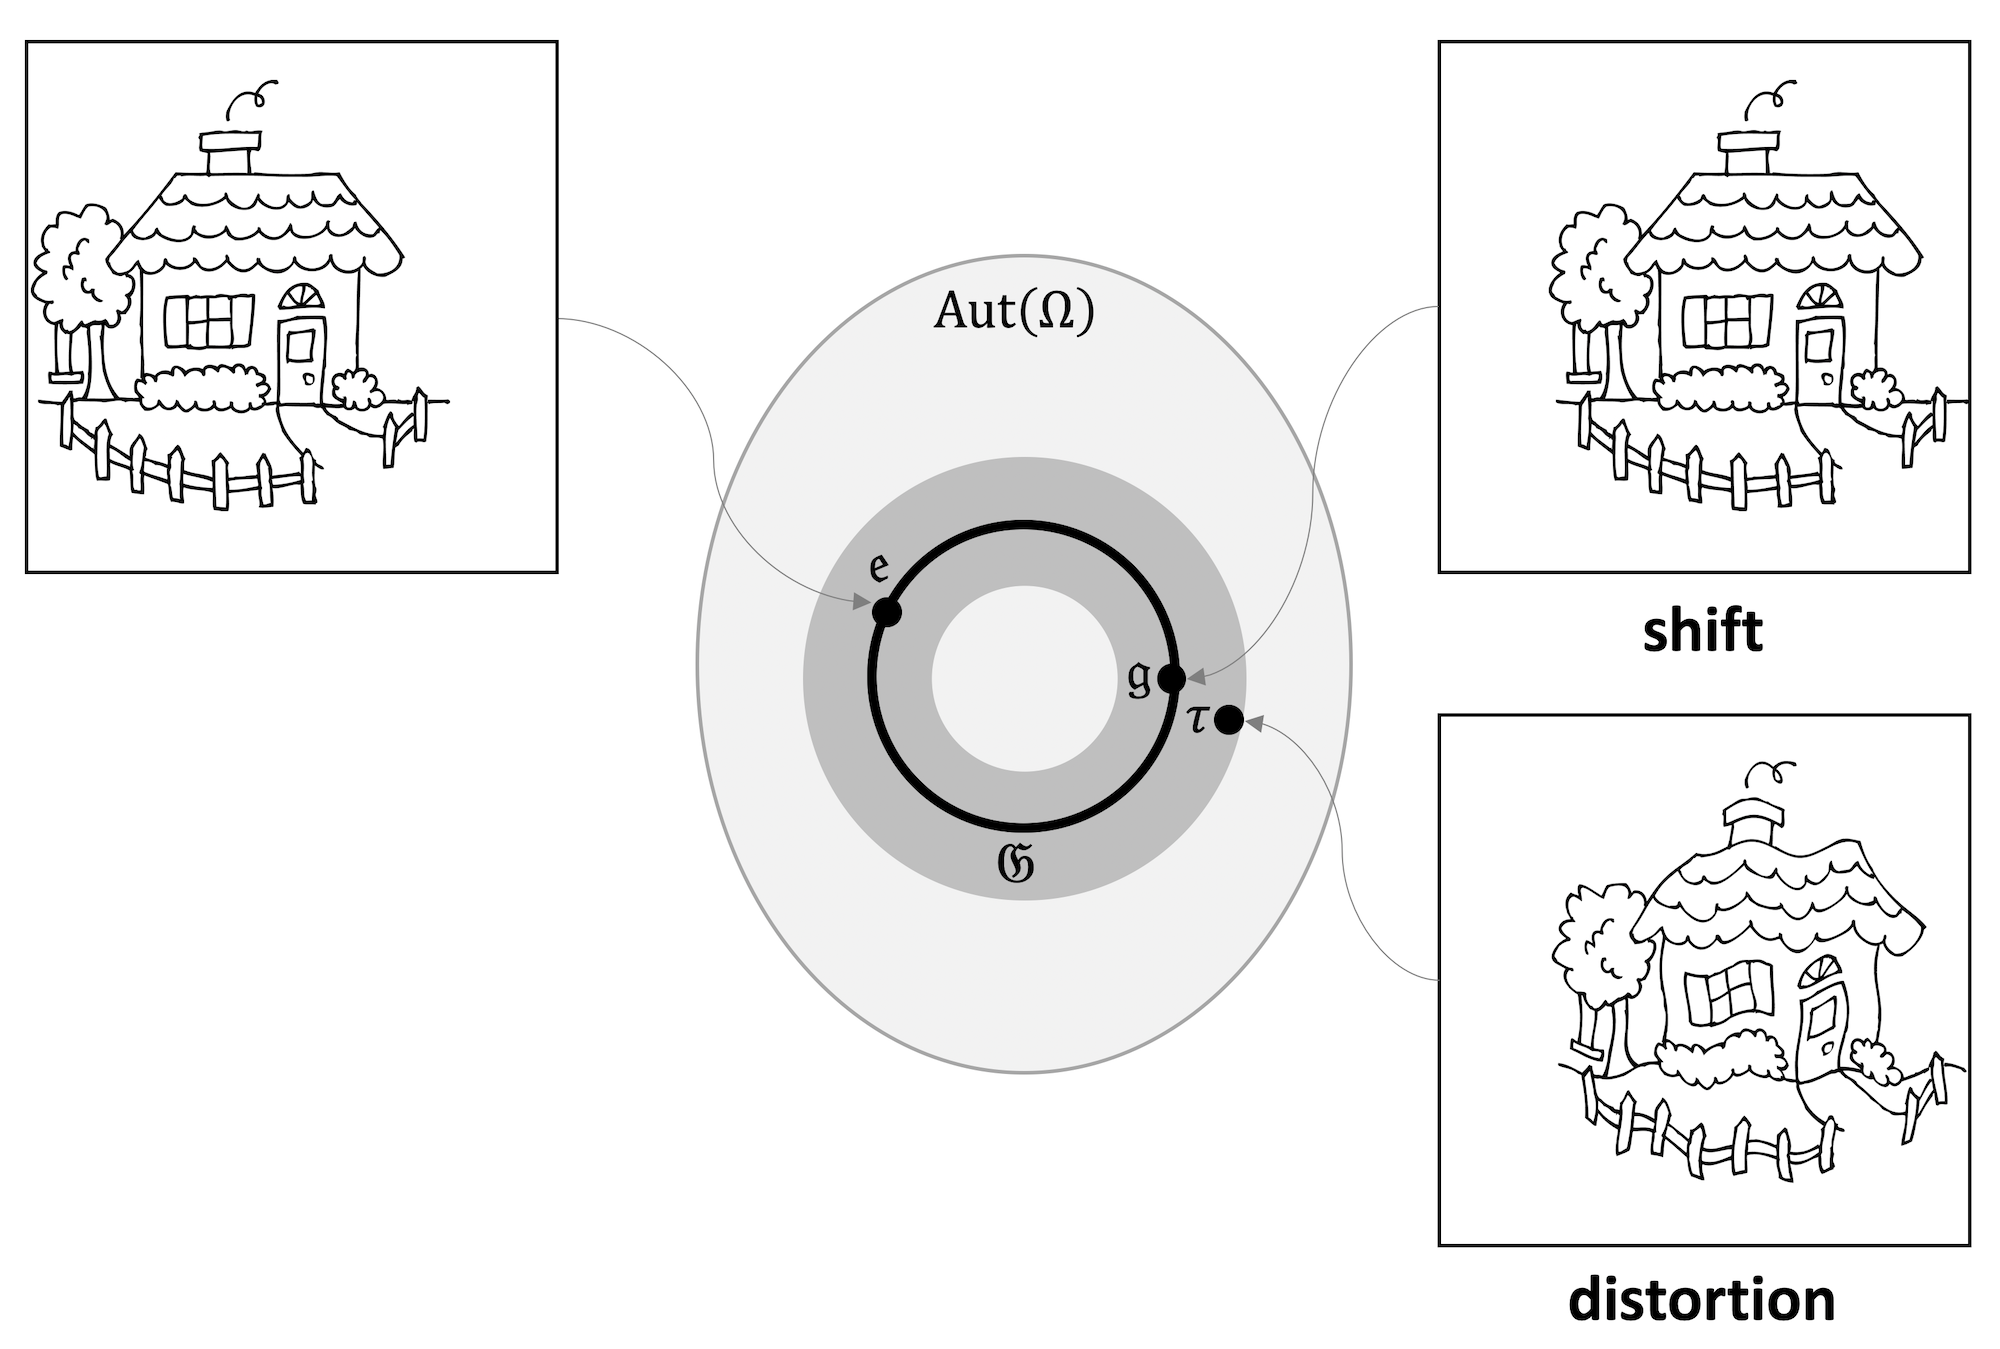
\includegraphics[width=1\textwidth]{figures/g_autg.png}
    \caption{从 $\Omega$ 到其自身的所有双射构成\emph{集自同构群} $\mathrm{Aut}(\Omega)$，对称群 $\fG$（图中圆形）是它的子群。几何稳定性把 $\fG$-不变性与等变性的概念推广到“$\fG$ 周围的变换”（图中灰色圆环）；这种邻近关系由变换之间的某种度量来量化。
    在本例中，图像的光滑畸变接近一次平移。
    }
    \label{fig:groupdeformation}
\end{figure}

%\begin{figure}
%    \centering
%    \includegraphics[width=0.7\textwidth]{figures/deform_image.pdf} \\
%    \includegraphics[width=0.7\textwidth]{figures/shapedef.pdf} \\
%        \includegraphics[width=0.4\textwidth]{figures/protein.jpg}
%    \caption{Examples of Deformations across different domains with a strong 
%    geometric stability prior. \michael{Better show a small molecule with a rotamer? Perhaps show just two examples of each?} }
%    \label{fig:deformation}
%\end{figure}

\paragraph{对域形变的稳定性}
在许多应用中，发生形变的对象不是信号，而是几何域 $\Omega$ 本身。处理图和流形的应用是典型实例：图可以对不同时刻、包含略有不同社会关系（关注图）的社交网络建模；流形则可以对经历非刚性形变的三维对象建模。
%The intuition that one can slightly bend or twist a manifold can be formalized by considering a 
这种形变可以按如下方式量化。若 $\mathcal{D}$ 表示所有可能的可变域空间（例如所有图的空间或 Riemann 流形空间），则可以对 $\Omega, \tilde{\Omega} \in \mathcal{D}$ 定义适当的度量（“距离”）$d(\Omega, \tilde{\Omega})$，并要求 $d(\Omega,\tilde{\Omega})=0$ 在 $\Omega$ 与 $\tilde{\Omega}$ 于某种意义下等价时成立。例如，当两个图同构时，图编辑距离为零；当两个配备测地距离的 Riemann 流形等距时，它们之间的 Gromov-Hausdorff 距离为零。\marginnote{图编辑距离衡量通过一系列图编辑操作使两个图同构所需的最小代价。Gromov-Hausdorff 距离衡量两个度量空间之间某种对应关系可能达到的最小度量畸变；见 \cite{gromov1981structures}。}


构造这类域间距离的一种常见方法依赖于某个可逆映射族
%We assume that this metric comes with an 
$\eta: \Omega \to \tilde{\Omega}$，它试图以尽可能保持相应结构的方式“对齐”这些域。%This can be quantified for, %that is,
例如，对于图或 Riemann 流形（将其视为带测地距离的度量空间），这种对齐可以比较成对的邻接结构或距离结构（分别为 $d$ 和 $\tilde{d}$），%the alignment of graphs
%two graphs with $n$ nodes can be aligned 
%
$$d_{\gD}(\Omega, \tilde{\Omega}) =  \inf_{\eta \in \fG}\|d - \tilde{d}\circ (\eta \times \eta)\|$$
%
%$$d(\Omega, \Omega') = \inf_{\eta \in \fG} %\| e(\Omega) - \eta e(\Omega') \|~,$$
其中 $\fG$ 是由双射或等距变换等同构组成的群，而范数定义在乘积空间 $\Omega \times \Omega$ 上。换言之，通过考虑所有保持内部结构的可能对齐，元素 $\Omega,\tilde{\Omega}$ 之间的距离被“提升”为域本身之间的距离。
%rigid 
%symmetries of the domain 
%(e.g. permutations for graphs, or isometries for Riemannian manifolds), and $e(\cdot)$ is an embedding of the domain (such as the adjacency matrix for a graph, or an Euclidean embedding for a manifold). 
%\michael{Joan: please check. The assumptions on $\eta$ e.g. in GH-metric are very weak, just a bijection}
\marginnote{可以通过二次指派问题（QAP）对齐两个图；在最简单的形式中，它考虑两个图 $G,\tilde{G}$，二者大小相同，均为 $n$，并求解 $\min_{\mathbf{P} \in \Sigma_n} \mathrm{trace}(\mathbf{A P \tilde{A} P}^\top)$，其中 $\mathbf{A}, \tilde{\mathbf{A}}$ 分别为邻接矩阵，$\Sigma_n$ 是 $n \times n$ 置换矩阵群。图编辑距离可以与这类 QAP 联系起来 \citep{bougleux2015quadratic}。
}
给定信号 $x \in \gX(\Omega)$ 和形变后的域 $\tilde{\Omega}$，便可以考虑形变后的信号 $\tilde{x} = x \circ \eta^{-1} \in \gX(\tilde{\Omega})$。
%, $x' := x \circ \varphi^{-1}$.  
%For example, we can define a metri

%metric \emph{in the space of domains}. In other words, two graphs %$G, G'$ can be assigned a distance $d(G,G')$ so that $d(G,G')=0$ iff $G$ and $G'$ are isomorphic, and similarly two Riemannian manifolds $\Omega, \Omega'$ can be compared so that $d(\Omega, \Omega')$ measures the changes in their intrinsic metric structure. 

稍微滥用一下记号，将 $\gX(\mathcal{D}) = \{ (\gX(\Omega), \Omega) \, : \, \Omega \in \mathcal{D} \}$ 定义为在可变域上定义的所有可能输入信号的集合。
如果函数 $f : \gX(\mathcal{D}) \to \gY$ 满足
\begin{equation}
\| f( x, \Omega) - f(\tilde{x}, \tilde{\Omega}) \| \leq C \|x \| d_{\gD}(\Omega, \tilde{\Omega})~
\label{eqn:domain_def_stability}
\end{equation}
%
且该式对所有 $\Omega, \tilde{\Omega} \in \mathcal{D}$ 以及 $x \in \mathcal{X}(\Omega)$ 都成立，则称其对域形变稳定。
%
%\michael{This is not properly defined: we have $x$ defined on both $\Omega$ and $\Omega'$, which requires some notion of correspondence} \joan{added some clarifications}. 
第~\ref{sec:manifolds}--\ref{sec:meshes} 节将在流形语境下讨论这一稳定性概念，其中等距形变起关键作用。
%As we will see in Chapter ??, 
此外，把信号形变稳定性理解为体积形式的形变，可以证明域形变稳定性是信号形变稳定性的自然推广 \cite{gama2019diffusion}。

% %Link between the two via a change of variables. 
% In fact, the two notions of deformation stability are intimately related. Indeed, the deformation operator $L_\tau : \gX \to \gX$ acting on signals can be recast as deforming the inner-product metric, from $\gX = L^2(\Omega, du)$ to $L^2(\Omega,du_\tau)$. In other words, 
% $$\langle L_\tau x, L_\tau y \rangle_{L^2(\Omega), du)} = \int_\Omega x(\tau^{-1}(u)) y(\tau^{-1}(u)) du = \int_\Omega x(u) y(u) |\mathbf{I} - \nabla \tau^{-1}(u) | du := \int_\Omega x(u) y(u) du_\tau~,$$
% so we may view certain signal deformations as specific perturbations of the metric. 

%\michael{Measure not metric? or volume form? I find this section more confusing than helpful, we need to introduce a lot of extra stuff to make it defined properly} \joan{yes, agreed, i simply put a pointer for the future chapter to simplify things for now}. 



\subsection{尺度分离}
\label{sec:scale_separation}

尽管形变稳定性显著增强了全局对称性先验，但它本身仍不足以克服维数灾难；非正式地说，随着域的规模增长，满足式 (\ref{eq:defstability1}) 的函数仍然“太多”。克服这一困难的关键洞见是利用物理任务的多尺度结构。在描述多尺度表示之前，需要先介绍依赖频率而非尺度的 Fourier 变换之主要要素。

\paragraph{Fourier 变换与全局不变量}
可以说，
\marginnote{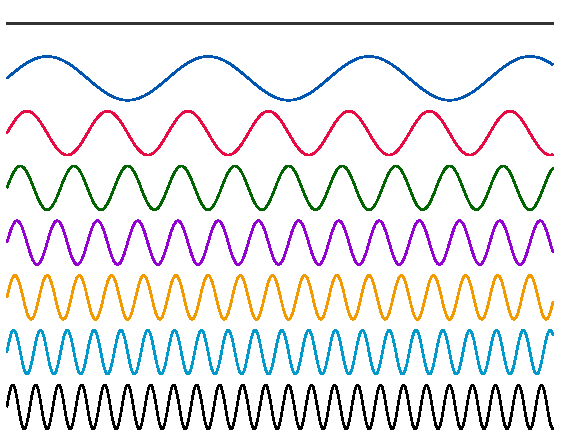
\includegraphics[width=\linewidth]{figures/fourier_basis.pdf}
Fourier 基函数具有全局支撑。因此，局部信号会在所有频率上产生能量。
}
最著名的信号分解是{\em Fourier 变换}，它是调和分析的基石。
%
经典的一维 Fourier 变换
$$
\hat{x}(\xi) = \int_{-\infty}^{+\infty} x(u) e^{-\mi \xi u} \mathrm{d}u
$$
把函数 $x(u) \in L^2(\Omega)$（定义在域 $\Omega = \mathbb{R}$ 上）表示为正交振荡{\em 基函数} $\varphi_\xi(u) = e^{\mi\xi u}$ 的线性组合，
并以它们的振荡速率（或\emph{频率}）$\xi$ 作为索引。按频率组织信号能够揭示其光滑性和局部化等重要信息。
%
%As we will show in Chapter ??, 
Fourier 基本身具有深刻的几何基础，可以解释为域的自然振动，并与域的几何结构相关（例如见 \cite{berger2012panoramic}）。
%\marginnote{Technically, the Fourier transform is defined for functions in $L^2(\Omega) \cup L^1(\Omega)$, and can be extended to a far broader class of generalised functions through the theory of {\em tempered distributions} developed by the Fields laureate Laurent Schwartz. 
%We refer to \cite{mckean} for a wonderful treatment of Fourier Analysis

%

%\begin{figure}
%    \centering
%\includegraphics[width=0.5\linewidth]{figures/fourier1.pdf}
%    \caption{Basic decomposition of a signal into Fourier atoms. Observe that a localized discontinuity in the original signal produces energy across all frequencies.}
%    \label{fig:fourier}
%\end{figure}


%

% \joan{Michael, let me know if you agree. The following paragraph is not strictly needed in this section, and rather belongs to the grid/euclidean domain where we go again through this. I suggest we merge in there.} 
Fourier 变换\marginnote{下文将把卷积与{\em （互）相关}
$$
(x \, \star \,\theta)(u) = \int_{-\infty}^{+\infty} \hspace{-2mm} x(v)\theta(u+v) \mathrm{d}v
$$
互换使用，这在机器学习中十分常见：二者的区别在于滤波器是否反射；由于滤波器通常是可学习的，因此这种区别纯粹只是记号上的。
}在信号处理中起关键作用，因为它给出了{\em 卷积}的对偶表述：
$$
(x\star \theta)(u) = \int_{-\infty}^{+\infty} x(v)\theta(u-v) \mathrm{d}v
$$
这是线性信号滤波的标准模型（这里及下文中，$x$ 表示信号，$\theta$ 表示滤波器）。
%
如下文将说明的，卷积算子在 Fourier 基下被对角化，因此可以把卷积表示为相应 Fourier 变换的乘积：
$$
\widehat{(x\star \theta)}(\xi) = \hat{x}(\xi) \cdot \hat{\theta}(\xi),
$$
这一事实在信号处理中称为卷积定理。
%
%In machine learning, convolution is the cornerstone of Convolutional Neural Networks, an architecture ubiquitously used in computer vision and image analysis applications. 


%Some of the properties of the Fourier transform are intimately related to the geometric properties of the Euclidean space or a grid on which it is defined.    
%The Fourier basis thus diagonalises any convolutional operator. 
事实证明，Laplacian 等许多基本微分算子都可以描述为欧氏域上的卷积。
%, such as the Laplacian $\Delta = \mathrm{div} \, \nabla$. 
由于这类微分算子可以在非常一般的几何上内蕴地定义，因此这提供了一种正式过程，可将 Fourier 变换推广到欧氏域之外，包括图、群和流形。第~\ref{sec:manifolds} 节将对此进行详细讨论。%Chapter~???.

Fourier 变换的一个本质特征是揭示信号与域的\emph{全局}性质，例如光滑性或传导率。当域具有平移等全局对称性时，这种全局行为十分便利，却不适合研究更一般的微分同胚。为此，需要一种能够权衡空间局部化与频率局部化的表示，下面将对此说明。


\paragraph{多尺度表示}
通过
%\marginnote{
%\includegraphics[width=0.9\linewidth]{figures/wavelet.pdf}
%Basic decomposition of a signal into wavelet atoms. Observe that now a localized discontinuity in the original signal creates energy only in the neighborhood of the discontinuity. 
从基于 Fourier 频率的表示切换到{\em 基于尺度的}表示，可以明确表达局部不变性的概念；这种表示是{\em 小波}等多尺度分解方法的基石。\marginnote{全面介绍见 \cite{mallat1999wavelet}。}
%; see Figure \ref{fig:fourier_vs_wavelets} and Insert ??. 
%
多尺度方法的核心洞见，是把定义在域 $\Omega$ 上的函数分解为\emph{在空间和频率上都局部化的}基本函数。\marginnote{
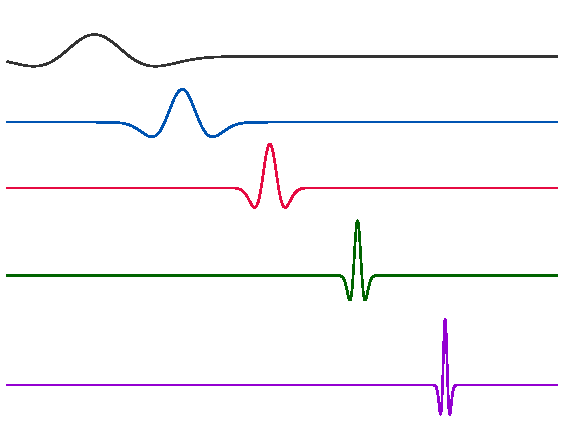
\includegraphics[width=0.9\linewidth]{figures/wavelet_basis.pdf}
%\includegraphics[width=0.9\linewidth]{figures/wavelet.pdf}
与 Fourier 原子不同，小波原子具有局部性和多尺度性，因此可以用空间支撑较小的原子捕获
信号的精细细节，并用空间支撑较大的原子捕获
粗略细节。
%Localized signals create energy only in the neighborhood of the discontinuity. 
这里的\emph{原子}一词与 Fourier 分析中的“基元素”同义，但需要注意，小波是冗余的（过完备的）。
}
对于小波，这是通过与经过平移和伸缩的滤波器（{\em 母小波}）$\psi$ 作相关来实现的，由此产生称为{\em 连续小波变换}的联合时频表示
%
$$
(W_\psi x)(u,\xi) = \xi^{-1/2} \int_{-\infty}^{+\infty} 
\psi\left(\frac{v-u}{\xi}\right) x(v) \mathrm{d}v.
%psi( 2^{j} (u - k2^{-j})) 
%x(u) du \marginnote{In general, $\psi$ can be a complex-valued function, in which case a complex conjugation must be taken in the inner product.}
%(x \star \psi_j)(u)
$$
%
经过平移和伸缩的滤波器称为{\em 小波原子}；% \marginnote{The term \emph{ atom} here is synonymous with `basis element' in Fourier analysis, with the caveat that wavelets are redundant representations that form over-complete bases.}
其空间位置与伸缩分别对应小波变换的坐标 $u$ 和 $\xi$。
%
这些坐标通常按二进方式采样（$\xi=2^{-j}$ 且 $u = 2^{-j}k$），其中 $j$ 称为{\em 尺度}。
%
%
%\int_{-\infty}^{+\infty} 
%\psi( 2^{j} (u - k2^{-j})) 
%x(u) du \marginnote{In general, $\psi$ can be a complex-valued function, in which case a complex conjugation must be taken in the inner product.}
%(x \star \psi_j)(u)
%$$
%
多尺度信号表示在捕获超越全局光滑性的正则性性质（例如分片光滑性）方面具有重要优势，这使其在二十世纪九十年代成为信号与图像处理以及数值分析中的常用工具。

\paragraph{多尺度表示的形变稳定性：}
当考虑底层对称群“附近”的小形变所产生的影响时，多尺度局部化小波分解相对于 Fourier 分解的优势便显现出来。下面在欧氏域和平移群中说明这一重要概念。
由于 Fourier 表示对角化了移位算子（正如第~\ref{sec:grids_euclidean} 节将更详细说明的，该算子可以视为卷积），因此它是平移变换的高效表示。然而，Fourier 分解在高频形变下并不稳定。
%
相比之下，小波分解在这类情形中提供了稳定表示。

事实上，考虑 $\tau \in \mathrm{Aut}(\Omega)$ 及其相关线性表示 $\rho(\tau)$。当 $\tau(u) = u - v$ 是一次平移时，
正如第 \ref{sec:grids_euclidean} 节将验证的，算子 $\rho(\tau) = S_v$ 是与卷积可交换的{\em 移位算子}。
%any convolution operator $H$ of the form $H x = x \star h$, with arbitrary filter $h$. 
由于卷积算子由 Fourier 变换对角化，频域中的平移作用等价于移动 Fourier 变换的复相位：
%
%As a result, by expressing this commutation relationship in the Fourier domain, we have that 
$$
(\widehat{S_v x})(\xi) = e^{-\mi \xi v} \hat{x}(\xi). 
$$ 
%for any frequency $\xi$. 
%Rigid translations are thus expressed in the Fourier domain by simply shifting the (complex) phase of every fourier coefficient of the signal, leading 
因此，去除复相位的{\em Fourier 模} $f(x) = |\hat{x}|$ 是一个简单的平移不变函数，即 $f(S_v x) = f(x)$。
%to simple translation invariant representations by removing this complex phase: $Mx = |\hat{x}|$. In other words, for rigid translations, the Fourier modulus is translation invariant: $\| M - M L_\tau \| = 0$. 
%
然而，如果只有近似平移，
%$\tau(u) \approx u - v$, 
$\tau(u) = u - \tilde{\tau}(u)$ 且 $\|\nabla \tau \|_\infty = \sup_{u\in \Omega} \| \nabla \tilde{\tau}(u)\| \leq \epsilon$，
情况便完全不同：可以证明
$$
\frac{\|f(\rho(\tau) x) - f(x) \| }{ \|x\| }= \mathcal{O}(1)
$$ 
无论 $\epsilon$ 多小（即 $\tau$ 多么接近一次平移），上述结论都成立。因此，这种 Fourier 表示在形变下{\em 不稳定}，无论形变多小。这种不稳定性也出现在一般域和非刚性变换中；第 \ref{sec:geomanifoldsec} 节将使用 Fourier 变换的自然推广分析三维形状，并看到另一个不稳定性实例。

小波为这一问题提供了补救方法，也揭示了多尺度表示的力量。在上述例子中，可以证明 \citep{mallat2012group} 小波分解 $W_\psi x$ 对形变{\em 近似等变}：
$$
\frac{\| \rho(\tau) (W_\psi x) - W_\psi (\rho(\tau) x) \|}{\|x\|} = \mathcal{O}(\epsilon).
\marginnote{This notation implies that $\rho(\tau)$ acts on the spatial coordinate of $(W_\psi x)(u,\xi)$.
}
$$
%and $\gW x = \{ x \star \psi_j \}_j$ is an appropriately normalized wavelet filter bank, then one can verify that wavelet coefficients are nearly \emph{equivariant} to deformations, in the sense that $\| L_\tau \gW - \gW L_\tau \| = O(\epsilon)$. 
%
换言之，使用局部化滤波器而不是频率把信号信息分解到不同尺度，会把全局不稳定表示转化为一族局部稳定特征。重要的是，不同尺度上的这类测量尚不具有不变性，需要逐步向低频处理；这暗示了现代神经网络深层组合的本质，并由下面给出的几何深度学习蓝图加以刻画。


% From our discussion 
% Let us consider a filter $h(u)$ and its associated convolution operator $\gH x = x \star h$. To study how this operator behaves under certain geometric transformations $L_\tau \in \mathrm{Aut}(\Omega)$ we consider the \emph{Lie commutator} 

% Let us consider the Lie commutator $[L_\tau, \gW]= L_\tau \gW - \gW L_\tau$. When $\gW$ is the Fourier transform and $L_\tau$ is exactly a translation, we have $[L_\tau, \gW] = 0$; 
% %Let us denote the decomposition by $U$ and let $L_\tau$ be the deformation operator we have seen before. When $\tau(u) = u-v$ is a pure translation, the Fourier transform satisfies $L_\tau U = U L_\tau$, by virtue of its 
% however when $L_\tau$ is only an approximate translation, then $\| [L_\tau, \gW] \| = O(1)$, irrespective of how close $L_\tau$ is to being a translation. 
% On the other hand, if $\tau(u) = u - \tilde{\tau}(u)$, with $\sup_u \| \nabla \tilde{\tau}(u)\| \leq \epsilon$ (thus $\tau$ is nearly a translation), then one can show \cite{scatt} that when $\gW$ is the overcomplete wavelet transform, $\| [ L_\tau, \gW ] \| \simeq \epsilon$. 





%\paragraph{Scale Separation}
%In our context of high-dimensional learning, multiscale representations such as wavelets serve another fundamental purpose: they provide overcomplete linear decompositions where local translations are nearly equivariant.  
\paragraph{尺度分离先验：}
基于这一洞见，可以考虑把数据域 $\Omega$ 多尺度粗化为层次结构 $\Omega_1, \hdots, \Omega_J$。
%, $j\in [J]$. 
事实证明，这类粗化可以在非常一般的域上定义，包括网格、图和流形。
%capturing a wide range of applications.
非正式地说，粗化把邻近点 $u, u' \in \Omega$ 合并在一起，因此只要求域中具有适当的{\em 度量}概念。
%Geometric objects such as grids, manifolds, Lie groups or Graphs all admit such coarsenings. 
如果 $\gX_{j}(\Omega_j,\mathcal{C}_j) := \{x_j: \Omega_j \to \mathcal{C}_j \}$
%\michael{\bf [MB: why $\R^s$? did not we assume scalar-valued signals for simplicity? ]} 
%\joan{JB: number of channels can vary as we coarsen the domain. But we should keep things simple at this stage, and just describe the general principle without introducing too much notation. } \michael{MB: lets keep it as simple as possible here} 
表示定义在粗化域 $\Omega_j$ 上的信号，那么非正式地说，若函数 $f : \gX(\Omega) \to \gY$ 在尺度 $j$ 上具有形式为 $f \approx f_j \circ P_j $ 的分解，其中 $P_j : \gX(\Omega) \to \gX_{j}(\Omega_j)$ 是非线性\emph{粗粒化}，而 $f_j : \gX_{j}(\Omega_j) \to \gY$，则称该函数在这一尺度上\emph{局部稳定}。换言之，虽然目标函数 $f$ 可能依赖整个域上特征之间复杂的长程交互，但对于局部稳定函数，可以\emph{分离}跨尺度交互：先关注局部化交互，再把它们向较粗尺度传播。

\begin{figure}
    \centering
    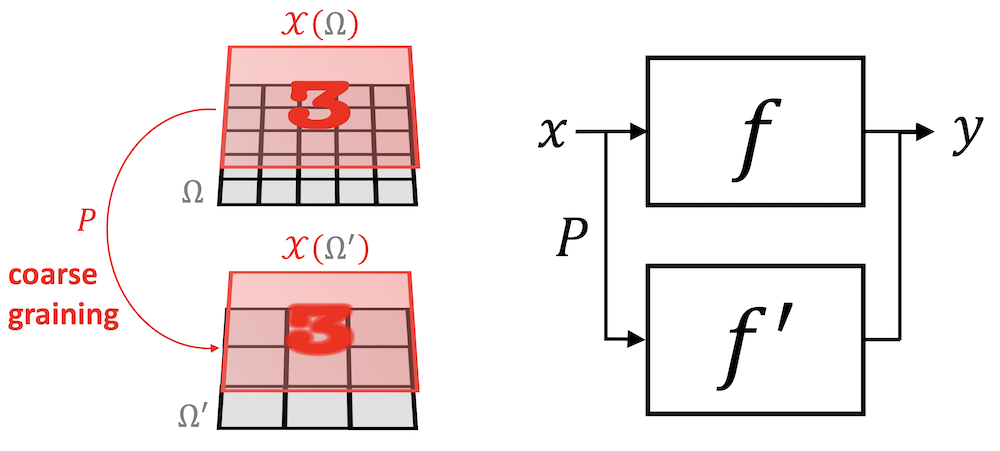
\includegraphics[width=0.75\textwidth]{figures/scale_sep.png}%factorization.pdf}
    \caption{图像分类任务中的尺度分离示意图。分类器 $f'$ 定义在粗网格信号 $\mathcal{X}(\Omega')$ 上，并应满足 $f \approx f'\circ P$，其中 $P: \mathcal{X}(\Omega) \rightarrow \mathcal{X}(\Omega')$。}
    \label{fig:scale_separation}
\end{figure}

这类原则\marginnote{Fast Multipole Method（FMM）是一种数值技术，最初用于加速 $n$ 体问题中长程力的计算。FMM 把彼此接近的源组合起来，并将其视为单一源。
}在物理学与数学的许多领域中具有根本重要性，例如体现在统计物理学所谓的重整化群中，或被 Fast Multipole Method 等重要数值算法利用。在机器学习中，多尺度表示与局部不变性是卷积神经网络和图神经网络高效性的底层基本数学原则，通常以{\em 局部池化}形式实现。在未来工作中，我们将进一步发展计算调和分析工具，在各种几何域上统一这些原则，并阐明尺度分离在统计学习中的优势。





\subsection{几何深度学习蓝图}
\label{sec:gdl_blueprint}

第~\ref{sec:symmetries}--\ref{sec:scale_separation} 节讨论的对称性、几何稳定性与尺度分离原则，可以组合为学习高维数据稳定表示的通用蓝图。
%
这些表示由函数 $f$ 产生；该函数作用于信号 $\mathcal{X}(\Omega,\mathcal{C})$，信号定义在域 $\Omega$ 上，而该域配备对称群 $\fG$。


目前描述的几何先验并未规定构建这类表示的具体{\em 架构}，而是给出了一系列必要条件。
不过，它们暗示了一种公理化构造；可以证明该构造满足这些几何先验，同时保证表示具有很强的表达能力，能够逼近任何满足这类先验的目标函数。%the geometric priors.


一个简单的初步观察是，为得到表达能力很强的表示，必须引入非线性元素，因为
如果 $f$ 是线性的且具有 $\fG$-不变性，那么对所有 $x \in \gX(\Omega)$，\marginnote{这里，$\mu(\fg)$ 称为群 $\fG$ 的\emph{Haar 测度}，积分在整个群上进行。}
$$
f(x) =  \frac{1}{\mu(\fG)} \int_{\fG} f( \fg. x) \mathrm{d}\mu(\fg) = f\left(\frac{1}{\mu(\fG)} \int_{\fG} (\fg.x) \mathrm{d}\mu(\fg) \right),
$$
%\michael{f(x) and not F?}
%\michael{what is $\fg.x$? should be u or use representation $\rho$}
这表明，$F$ 对 $x$ 的依赖仅通过\emph{$\fG$-平均} $A{x} = \frac{1}{\mu(\fG)} \int_{\fG} (\fg.x) \mathrm{d}\mu(\fg)$ 实现。对于图像和平移，这意味着只使用输入的平均 RGB 颜色！%\marginnote{Give a further example for the discrete permutation group, getting the average too}


尽管这一推理表明{\em 线性不变量}族并不丰富，但{\em 线性等变映射}族提供了强大得多的工具，因为通过与适当的非线性映射复合，它能够构造丰富且稳定的特征，下面将对此说明。
%
事实上，若 $B: \gX(\Omega, \gC) \to \gX( \Omega, \gC')$ 具有 $\fG$-等变性，并满足 $B(\fg.x) = \fg.B(x)$，且该式对所有 $x \in \gX$ 和 $\fg \in \fG$ 都成立；再令 $\sigma: \gC' \to \gC''$ 为任意（非线性）映射，则容易验证，复合 $U := (\bm{\sigma} \circ B): \gX(\Omega, \gC) \to \gX( \Omega, \gC'')$ 也具有 $\fG$-等变性。其中，$\bm{\sigma}: \gX(\Omega,\gC') \to \gX(\Omega, \gC'')$ 是 $\sigma$ 的逐元素实例化，定义为 $(\bm{\sigma}(x))(u) := \sigma( x(u))$。

这一简单性质允许定义一个非常一般的 $\fG$-不变量族，方法是把 $U$ 与群平均 $A \circ U : \gX(\Omega, \gC) \to \gC''$ 复合。因此，一个自然问题是：任何 $\fG$-不变函数能否在适当选择 $B$ 和 $\sigma$ 后，由这类模型以任意精度逼近？
%
不难把针对非结构化向量输入的标准通用逼近定理加以调整：通过把群平均适当地推广为一般非线性不变量，可以证明浅层“几何”网络也是通用逼近器。
\marginnote{例如，\citet{zaheer2017deep} 已经为 Deep Sets 模型给出了这类证明。}
%
然而，正如比较 Fourier 不变量与小波不变量时已经说明的，
浅层全局不变性与形变稳定性之间存在根本张力。
这促使我们采用另一种表示，转而考虑\emph{局部化的}等变映射。\marginnote{可以在网格、图、流形和群上定义有意义的度量。一个显著例外是集合，它没有预先定义的度量概念。
%; see Section ? for further discussion.
} 
进一步假设 $\Omega$ 配备距离度量 $d$。若等变映射 $U$ 满足如下条件，则称其为局部化的：$(Ux)(u)$ 只依赖于 $x(v)$ 的值，其中 $\mathcal{N}_u = \{v : d(u,v) \leq r\}$，而 $r$ 是某个较小半径；后一集合 $\mathcal{N}_u$ 称为{\em 感受野}。%$\delta$; .
%\michael{Are we ok to indentify neighbourhood with receptive field?}

单层局部等变映射 $U$ 无法逼近具有长程交互的函数，但多个局部等变映射的复合 $U_J \circ U_{J-1} \dots \circ U_1$ 在保持局部等变映射稳定性性质的同时扩大了感受野\marginnote{“感受野”一词源自神经科学文献，指影响给定神经元输出的空间域。}。通过交错使用粗化域的下采样算子（仍假设具有度量结构），可以进一步扩大感受野，从而完整对应于多分辨率分析（MRA，例如见 \cite{mallat1999wavelet}）。

\begin{figure}
    \centering
    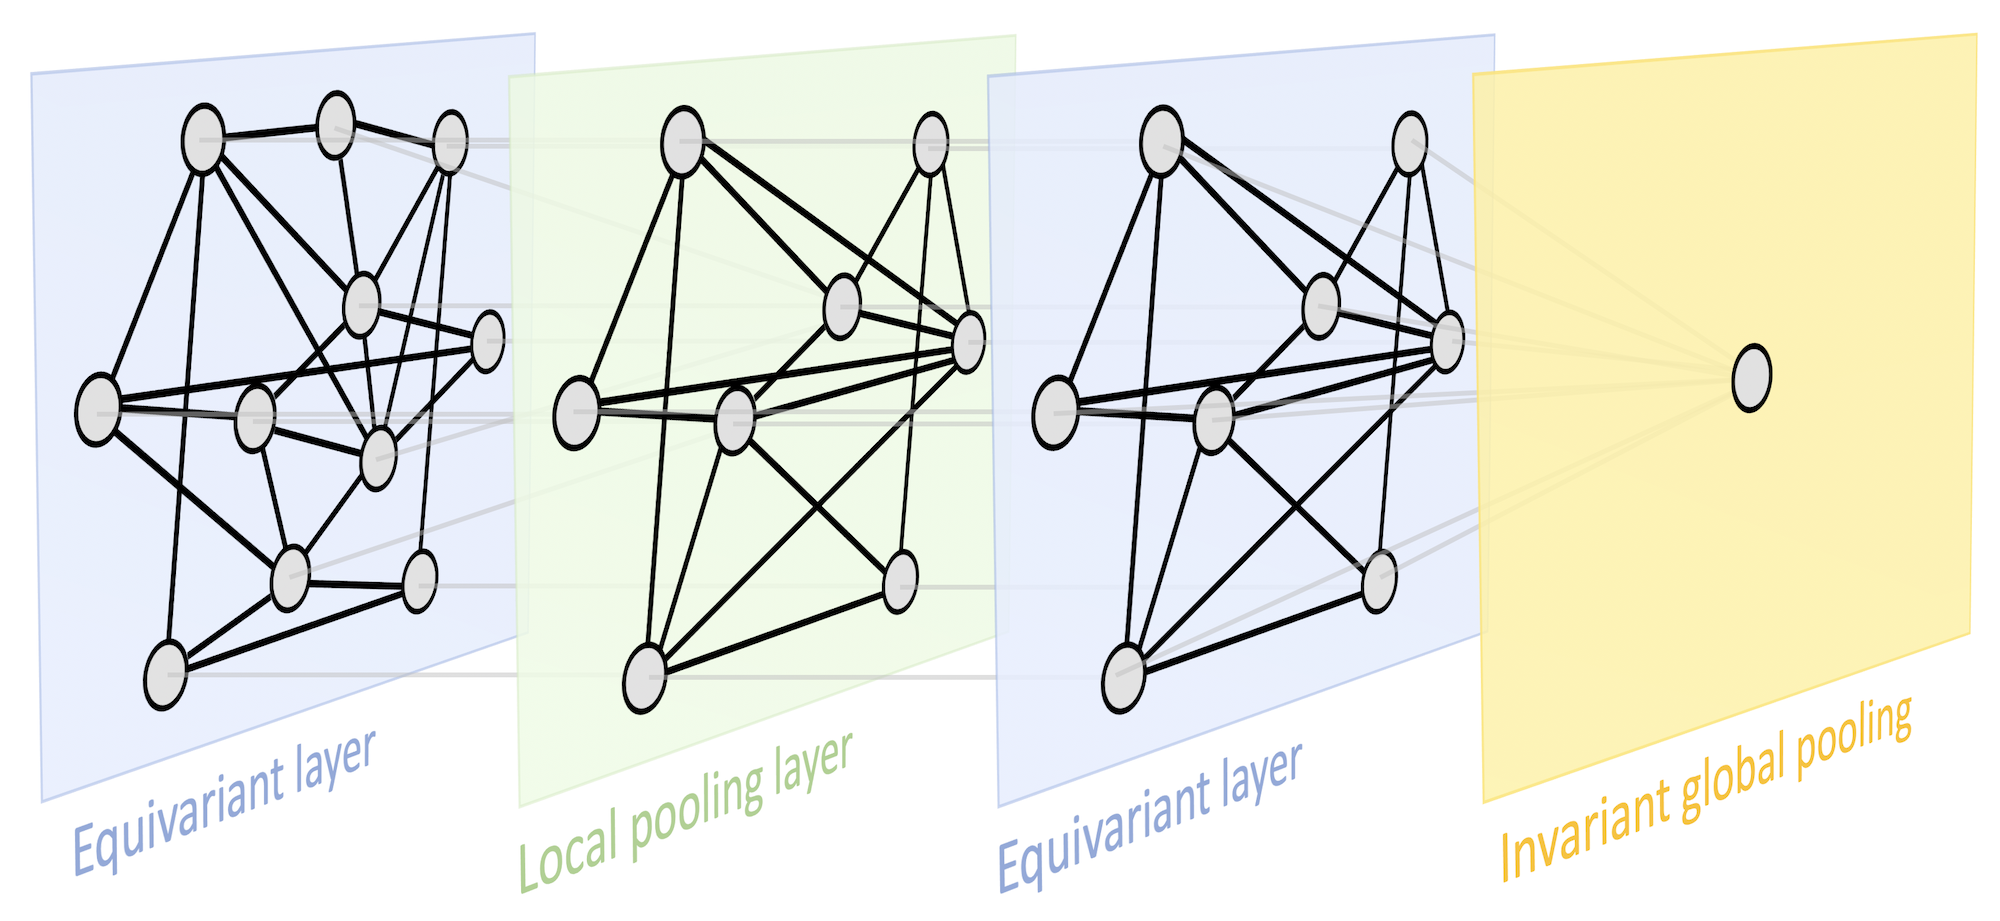
\includegraphics[width=1\textwidth]{figures/blueprint.png}
    \caption{以图为例说明的几何深度学习蓝图。典型的图神经网络架构可以包含置换等变层（计算逐节点特征）、局部池化（图粗化）以及置换不变的全局池化层（读出层）。}
    \label{fig:blueprint}
\end{figure}

总而言之，输入域的几何结构以及对其底层对称群的了解，给出了三个关键构件：（i）局部等变映射，（ii）全局不变映射，以及（iii）粗化算子。将这些构件组合在我们称为
%
\emph{几何深度学习蓝图}（图~\ref{fig:blueprint}）的方案中，即可得到一个具有预设不变性与稳定性性质的丰富函数逼近空间。
%
%We will see that a large number of popular neural network architectures used in deep representation learning are particular instances of this blueprint, illustrated in 
%across all the geometric domains we will describe next. 
%



%\begin{tcolorbox}[width=\linewidth,
%                  boxsep=0pt,
%                  left=7.5pt,
%                  right=7.5pt,
%                  top=7.5pt,
%                  bottom=7.5pt,
%                  arc=0pt,
%                  boxrule=0pt,toprule=0pt,
%                  colback=boxgray,
%                  ]%%
    
%\begin{center}
%Given a hierarchy of domains $\Omega_J \subseteq \hdots \subseteq \Omega_2 \subseteq \Omega_1 = \Omega$ with symmetry group $\fG$, the 
%\textbf{Geometric Deep Learning Blueprint} allows constructing $\fG$-invariant functions $f:\mathcal{X}(\Omega,\mathcal{C}) \rightarrow \mathcal{Y}$ of the form 
%$$
%f = A \circ \boldsymbol{\sigma}_J \circ U_J \circ P_{J-1} \circ \hdots \circ P_1 \circ \boldsymbol{\sigma}_1 \circ B_1
%$$
%consisting  of the following building blocks:\\

%    \noindent {\em Linear $\fG$-equivariant layer} $B_j: \gX(\Omega_j, \gC_j) \to \gX( \Omega_{j}, \gC'_{j})$ satisfying $B(\fg.x) = \fg.B(x)$ for all $\fg \in \fG$ and $x\in \gX(\Omega_j,\mathcal{C}_j)$. 
%    \vspace{2mm}\\

%    \noindent {\em Nonlinearity} $\sigma_j: \gC'_j \to \gC_j$ applied element-wise as $(\bm{\sigma}(x))(u) = \sigma( x(u))$.\vspace{2mm}\\\

%    \noindent {\em Local pooling (coarsening)}  $P_j : \gX(\Omega_j, \gC_j) \rightarrow \gX(\Omega_{j+1}, \gC_{j+1}) $.\vspace{2mm}\\
    
%    \noindent {\em Invariant layer (global pooling) } $A: \gX(\Omega_J, \gC_J) \rightarrow \mathcal{Y}$ satisfying $A(\fg .x) = A(x)$ for all $\fg \in \fG$ and $x\in \gX(\Omega_J,\mathcal{C}_J)$.  %.\vspace{2mm}\\

%\end{center}
%\end{tcolorbox}


\newpage
\begin{tcolorbox}[width=\linewidth,
                  boxsep=0pt,
                  left=7.5pt,
                  right=7.5pt,
                  top=4pt,
                  bottom=4pt,
                  arc=0pt,
                  boxrule=0pt,toprule=0pt,
                  colback=boxgray,
                  ]%%
\small
\begin{center}
\textbf{几何深度学习蓝图}
\end{center}
设 $\Omega$ 和 $\Omega'$ 为域，$\fG$ 为 $\Omega$ 上的对称群；我们用 $\Omega' \subseteq \Omega$ 表示 $\Omega'$ 可视为 $\Omega$ 的紧致版本。\\

我们定义如下构件：\vspace{2mm}\\

    \noindent {\em 线性 $\fG$-等变层} $B: \gX(\Omega, \gC) \to \gX( \Omega', \gC')$，满足 $B(\fg.x) = \fg.B(x)$，且该式对所有 $\fg \in \fG$ 和 $x\in \gX(\Omega,\mathcal{C})$ 均成立。\vspace{2mm}\\

    \noindent {\em 非线性} $\sigma: \gC \to \gC'$，按元素施加为 $(\bm{\sigma}(x))(u) = \sigma( x(u))$。\vspace{2mm}\\

    \noindent {\em 局部池化（粗化）} $P : \gX(\Omega, \gC) \rightarrow \gX(\Omega', \gC) $，其中 $\Omega'\subseteq\Omega$。\vspace{2mm}\\
    
    \noindent {\em $\fG$-不变层（全局池化）} $A: \gX(\Omega, \gC) \rightarrow \mathcal{Y}$，满足 $A(\fg .x) = A(x)$，且该式对所有 $\fg \in \fG$ 和 $x\in \gX(\Omega,\mathcal{C})$ 均成立。\vspace{2mm}\\

利用这些构件，可以构造如下形式的 $\fG$-不变函数 $f:\mathcal{X}(\Omega,\mathcal{C}) \rightarrow \mathcal{Y}$：
$$
f = A \circ \boldsymbol{\sigma}_J \circ B_J \circ P_{J-1} \circ \hdots \circ P_1 \circ \boldsymbol{\sigma}_1 \circ B_1
$$
其中，各构件的选择应使每个构件的输出空间与下一个构件的输入空间相匹配。不同构件可以利用不同的对称群 $\fG$ 选择。
\end{tcolorbox}

%


% A natural question is then how expressive this generic construction is in the class of $\fG$-invariant functions, and, equally important, which conditions on $B$ and $\rho$ ensure geometric stability.  
% Universal Approximation

% A simple option to ensure rich and stable representations is to instead compose several \emph{layers} of non-linear local equivariant maps before applying the global invariant. 

% The idea of deep learning is to define $f$ as a \emph{composition} of maps (or ``layers'').
% These maps should be compatible in that the output space of one layer should match the input space of the next layer.
% %That is, we can compose $f_1 : \mathcal{X}(\Omega, \mathcal{C}) \rightarrow \mathcal{X}(\Omega', \mathcal{C}')$ and $f_2 : \mathcal{X}(\Omega'', \mathcal{C}'') \rightarrow \mathcal{X}(\Omega''', \mathcal{C}''')$ if and only if $\mathcal{X}(\Omega', \mathcal{C}') = \mathcal{X}(\Omega'', \mathcal{C}'')$.
% That is, we can compose $f_1 : \mathcal{X}_1 \rightarrow \mathcal{X}_2$ and $f_2 : \mathcal{X}_2' \rightarrow \mathcal{X}_3$ if and only if $\mathcal{X}_2 = \mathcal{X}_2'$ (where we have abbreviated $\mathcal{X}_i = \mathcal{X}(\Omega_i, \mathcal{C}_i)$).
% Whereas in regular deep learning, maps can be composed as soon as the input and output spaces match as \emph{vector spaces} (i.e. they have the same dimensionality / array shape), in geometric deep learning these spaces should match as \emph{group representations}.
% This means that, in addition to matching as vector spaces, the group $\fG$ should act in the same way on both spaces.
% When this is the case, equivariance of $f_1$ and $f_2$ implies equivariance of the composition $f_2 \circ f_1$.

% Most networks in geometric deep learning are compositions of a few basic building blocks:

% %\emph{Local} 
% $\fG$-\emph{equivariant} linear operator $A: \gX(\Omega) \to \gX_{\gV'}(\Omega)$ satisfying $A(\fg.x) = \fg. A(x)$ for any $x \in \mathcal{X}(\Omega)$ and $\fg\in\fG$. 
% %
% Typically, this operator is further assumed to be {\em local}, i.e. $(Ax)(u)$ depends only on the values of $x(v)$ for $v$ in the vicinity of $u$, in the sense of some metric on $\Omega$.  
% %and such that $A x(u)$ only depends upon $\{ x(v); \mathrm{g}(v,u) \leq \delta\}$, where $\delta$ encodes the size of the neighborhood. 

% \emph{Pointwise nonlinearity} $\sigma: \mathcal{C}' \to \mathcal{C}''$. Under our assumptions, this implies that $\sigma \circ A$ is local and $\fG$-\emph{equivariant} whenever $A$ is such. \marginnote{When $\sigma$ acts coordinate-wise, it is typically referred to as an \emph{activation function}. In general,  $\sigma$ can be a generic function, such as a fully-connected neural network. }

% % \joan{
% % Argue that the only linear $\fG$-invariant is the group average. 
% % If $F$ is linear and $\fG$-invariant, then for all $x$, 
% % $$F(x) =  \frac{1}{\mu(\fG)} \int F( g.x) \mu(dg) = F\left(\frac{1}{\mu(\fG)} \int g.x \mu(dg) \right)~,$$
% % so $F$ only depends on $x$ through the average. 

% % This justifies why we need to add non-linearities
% % }




% {\em Local pooling} (or downsampling operator) $P_j: \gX(\Omega_j,\mathcal{C}_{j}) \to \gX(\Omega_{j+1},\mathcal{C}_{j+1})$ defined on a hierarchy of domains $\Omega_1, \hdots, \Omega_J$. 
% %reducing the resolution of the domain. 

% {\em Global pooling} $\fG$-{\em invariant} operator $a:\mathcal{X}(\Omega,\mathcal{C}) \rightarrow \mathcal{Y}$. 
    



% %
% %\michael{\bf [MB: INSERT FIGURE of a general equivariant/invariant architecture, similarly to Maron's thesis]}
% %
% %Let $\gX(\Omega, \gV) := \{ x : \Omega \to \gV \}$ be the input space, with domain $\Omega$ and feature space $\gV$ . We assume a metric $\mathrm{g}$ on $\Omega$ and a symmetry group $\fG$ acting on it, which also defines a linear representation 
% %%(taco confirm language? \taco{Correct. This is called the regular rep of G on X. Will add a definition to 1.2.1}) 
% %over $\gX$ by composition, as in Figure \ref{fig:symmetryactors}.
% %%if $x \in \gX$ and $g \in \fG$, then $g x (u) = x(gu) \in \R^s$. [we assume that the group does not act along channels for now]
% %\taco{TODO: add condition that signal space should have an inner product, i.e. be a Hilbert space. See definition box in 1.2}
% %
% %The GDL blueprint consists of four fundamental building blocks that are composed together appropriately:
% %\begin{enumerate}
% %    \item A \emph{local} $\fG$-\emph{equivariant} linear operator $A: \gX_{\gV}(\Omega) \to \gX_{\gV'}(\Omega)$; that is, $A(\fg.x) = \fg. A(x)$ for any $x$ and $\fg$, and such that $A x(u)$ only depends upon $\{ x(v); \mathrm{g}(v,u) \leq \delta\}$, where $\delta$ encodes the size of the neighborhood. 
% %    \item A \emph{nodewise} nonlinear activation function $\sigma: \gV' \to \gV''$. Under our assumptions, this implies that $\sigma \circ A$ is local and $\fG$-\emph{equivariant} whenever $A$ is as above. When $\text{dim}(\gV')=\text{dim}(\gV'')=1$, $\sigma$ is typically described as an \emph{activation function}, but in general $\sigma$ can be a generic function, such as a fully-connected neural network. 
% %    \item Local pooling or downsampling operator $P_k: \gX_{\gV}(\Omega_k) \to \gX_{\gV}(\Omega_{k+1})$ reducing the resolution of the domain. 
% %    \item Global pooling: $\fG$-invariant operator. 
% %\end{enumerate}




% %\michael{MB: I am in favor of keeping the blueprint as simple as possible even at the expense of precision of definitions/generality. It should be intuitive and I feel currently the intuition is buried under too much notation. }


% The majority of deep neural networks implement a composition of multiple such components of the form
% $$
% f =a \circ P_L \circ \sigma_L \circ A_L \dots P_1 \circ \sigma_1 \circ A_1,
% $$
% with each component referred to as a {\em layer}. The term `deep' is used to indicate that there are many such layers, though we should say that how deep is deep is in the eyes of the beholder.\marginnote{Some CNN architectures used in computer vision can have hundreds of layers. }
% %
% %The multilayer composition $f =a \circ P_L \circ \sigma_L \circ A_L \dots P_1 \circ \sigma_1 \circ A_1$ 
% %
% Such a multilayer construction allows to define a flexible functional space with prescribed geometric priors. On the one hand, the equivariant nature of the maps $\sigma \circ A_j$ is preserved under composition, resulting in overall invariance when composed with a global pooling operator. On the other hand, the use of pooling layers allows to exploit the scale separation prior. 

\paragraph{几何深度学习的不同设定}
这里可以作出一个重要区分：一种设定假定域 $\Omega$ {\em 固定}，仅关注定义在该域上的可变输入信号；另一种设定则将域作为输入的一部分，使其与定义于其上的信号一同{\em 变化}。
%
前一种情形的经典实例见于计算机视觉应用，其中图像被假定定义在固定域（网格）上。
%
图分类是后一种设定的例子，其中图的结构及定义在其上的信号（例如节点特征）都很重要。
%
在域可变的情形下，几何稳定性（即对 $\Omega$ 形变的不敏感性）在几何深度学习架构中起着关键作用。


该蓝图具有恰当的普适程度，可用于广泛的几何域。
因此，不同的几何深度学习方法在域、对称群的选择以及上述构件的具体实现细节上有所不同。
%and the metric defining locality. 
正如下文将看到的，目前使用的一大类深度学习架构都属于这一方案，因而可以从共同的几何原理导出。
%
%We will now discuss specific instances of this blueprint and how it adapts to each case.  


在以下各节（\ref{sec:proto-graphs}--\ref{sec:meshes}）中，我们将以“5G”为重点介绍各种几何域；在第~\ref{sec:cnnsec}--\ref{sec:lstm} 节中，则介绍几何深度学习在这些域上的具体实现。



%Such generic architecture, illustrated in Figure~\ref{fig:blueprint}, can be instantiated across a variety of domains with different geometric structures giving rise to a very large zoo of architectures united by these common geometric principles. Let us now discuss these domains and how this blueprint adapts to each case. 


% First, we define a collection of \emph{local} $\fG$-\emph{equivariant} linear operators. In  deep learning architectures such as CNNs and GNNs these correspond to convolutional and message passing layers, and the corresponding groups are translation and permutation, respectively. 

% Next, these operators are composed with a non-linearity called an {\em activation function} in the neural networks jargon, which preserves the equivariance as it is applied element-wise. \taco{TC: note that element-wise nonlinearities are only equivariant to certain kinds of group representations, namely when the representation matrices are all permutation matrices}

% Finally, coarsen the representations produced by the equivariant operators. In image analysis applications, this is achieved by means of {\em pooling}, an operation reducing the size of the image grid, and as we shall see next, coarsening may be defined on far more general data domains.

% In an idealised instantiation, the coarsening is performed at the output. It can be shown that this representation is 
% provably $\fG$-invariant/equivariant, and that the locality assumption captures the scale separation inductive bias. 
% Moreover, such representations are universal approximators under symmetry, as we discuss in Chapter ??. 

%\joan{Joan: Taco, we can generalise the blueprint to accommodate more group representations, if we feel the use cases are sufficiently important. Otherwise, an alternative is to mention that this blueprint can be extended in some domains to account for special types of group actions}

%\taco{Taco: Joan, I agree we really only need reps that describe how signals transform. However that is still a bit more general than $\rho(\fg) x(u) = x(\fg^{-1} u)$. In particular for steerable cnns / induced reps, as well as gauge cnns, we have some smaller group acting on the feature vector. E.g. a vector field on the sphere transforms according to the rep of SO3 that is induced by the vector rep of SO2 acting on 2D vectors. 

%One option is to ignore this for now and call this the ``deep learning blueprint (simplified)'', and mention that we need something slightly more general. We can introduce the full thing in a separate chapter. Only downside is that we cannot write the gauges section of the intro to conform to the simplified blueprint then. May not be such a big deal...

%Alternatively, we can first introduce a general definition for arbitrary reps, then introduce one specialized version for $\rho(\fg) x(u) = x(\fg^{-1} u)$. Then later we can say in the gauges section that the gauge story fits the general blueprint but involves a different kind of rep.
%}


%(either explicitly or implictly since energy is pushed towards low frequencies).
    

%\begin{enumerate}
%    \item Define a collection of \emph{local}, $\gG$-\emph{equivariant} linear operators $U_m$. 
%    \item Compose them with an element-wise non-linearity $\rho$. 
%    \item Coarsen the hidden representations (either explicitly or %implictly since energy is pushed towards low frequencies).
%\end{enumerate}





\begin{tcolorbox}[width=\linewidth,
                  boxsep=0pt,
                  left=7.5pt,
                  right=7.5pt,
                  top=7.5pt,
                  bottom=7.5pt,
                  arc=0pt,
                  boxrule=0pt,toprule=0pt,
                  colback=boxgray,
                  ]%%
    
\begin{center}
%\textbf{Geometric Deep Learning Blueprint}\newline
\begin{tabular}{lll}
     {\bf 架构} & {\bf 域} $\Omega$ & {\bf 对称群} $\mathfrak{G}$\vspace{2.5mm}\\
     {\em CNN} & 网格 & 平移\vspace{2mm}\\
%
     {\em 球面 CNN} & 球面 / $\mathrm{SO}({3})$ & 旋转 $\mathrm{SO}({3})$\vspace{2mm}\\

     {\em 内蕴 / 网格 CNN} & 流形 & 等距变换 $\mathrm{Iso}(\Omega)$ / \\
     & & 规范对称性 $\mathrm{SO}(2)$\vspace{2mm}\\


     {\em GNN} & 图 & 置换 $\Sigma_n$\vspace{2mm}\\

     {\em Deep Sets} & 集合 & 置换 $\Sigma_n$\vspace{2mm}\\
     {\em Transformer} & 完全图 & 置换 $\Sigma_n$\vspace{2mm}\\
     {\em LSTM} & 一维网格 & 时间扭曲\\


\end{tabular}
\end{center}
\end{tcolorbox}
%

%\begin{tcolorbox}[width=\linewidth,
%                  boxsep=0pt,
%                  left=7.5pt,
%                  right=7.5pt,
%                  top=7.5pt,
%                  bottom=7.5pt,
%                  arc=0pt,
%                  boxrule=0pt,toprule=0pt,
%                  colback=boxgray,
%                  ]%%
%    
%\begin{center}
%\textbf{Geometric Deep Learning Blueprint instances of interest}\newline
%\begin{tabular}{cccc}
%     Domain, $\Omega$ & Metric, $g$ & Symmetry group, $\frak{G}$ & Architecture\\
%     {\bf Grids} & $L_\infty$ & Translations & {\bf CNNs}\\ 
%     {\bf Spheres} & Great circle & \multirow{2}{*}{3D rotations, SO(3)} & \multirow{2}{*}{\bf Spherical CNNs} \\
%     {\bf SO(3)} & Geodesic & \\
%     \multirow{2}{*}{\bf Gauges} & \multirow{2}{*}{Geodesic} & \multirow{2}{*}{\{Gauge transform.\}} & {\bf Gauge Equivariant} \\ & & & {\bf Mesh CNNs} \\
%     {\bf Graphs} & Shortest path & Permutations, $\Sigma_n$ & {\bf GNNs}\\
%     \multirow{2}{*}{\bf Sets} & $+\infty$ & Permutations, $\Sigma_n$ & {\bf Deep Sets}\\
%     & $0$ & Permutations, $\Sigma_n$ & {\bf Transformers}\\
%\end{tabular}
%\end{center}
%\end{tcolorbox}


%\begin{figure}
%    \centering
%    \includegraphics[width=0.9\textwidth]{figures/equivariant-network-blueprint.png}
%    \caption{todo}
%    \label{fig:equivariant-net-blueprint}
%\end{figure}




%\michael{\bf [MB: give examples here?]}



%{\bf 
%Main questions:

%What the equivariant structure that is required at every hidden %layer. 
%Universality vs efficiency. 

%Generalization?
%}

%Scale separation in neural networks

%Graph isomorphism Gromov graphs

%Link to deformation stability. 

%\subsection{{Leveraging Geometric Structure}}

% \begin{itemize}
%     \item Two main universal principles: symmetries and scale separation. 
%     \item These two principles have deep long roots in physics and mathematics (homogeneization, Galois theory, Noether's theorem, etc etc etc)
%     \item They are omnipresent in many modern data domains: computer vision, physical systems, chemistry, networks.  
%     \item Can we make these principles compatible with large scale ML models (gradient-based learning)? 
%     \item Can we recover Universal approximation models while leveraging geometric structure. It turns out that Neural Networks are a good language for that since we can add symmetry and scale while preserving their universal approximation properties. 
% \end{itemize}


\section{几何域：5G}


%As already mentioned, the geometric priors of symmetry and scale separation can be instantiated across a broad range of geometric domains of increasing level of specialization. 
%
%Since the subtitle of our book is `4G', 

本文将重点讨论图、网格、群、测地线和规范。在这里，“群”是指齐性空间中的全局对称变换，“测地线”是指流形上的度量结构，而“规范”是指定义在切丛（以及一般向量丛）上的局部参考标架。
后文将更详细地解释这些概念。
%\marginnote{A {\em gauge} is a choice of frame (system of coordinates) for a collection of vector spaces attached to some base manifold, such as the tangent space to a manifold, or an RGB color vector attached to each position in a planar image. This term is used in physics. 
%}, and . % where `gauges' is a high-energy physics parlance for objects with manifold structure. 
%where grids can be considered 
%
%In this Section we introduce the main geometric domains 
%that will be the central focus of the book: Graphs, Grids, Gauges and Groups, 
%
在接下来的各节中，我们将详细讨论这些结构的主要共同要素与关键区别，并描述与之相关的对称群。
%
本文并不按普适性顺序展开——事实上，网格是图的特例——而是力求突出几何深度学习蓝图背后的重要概念。




\begin{figure}
    \centering
    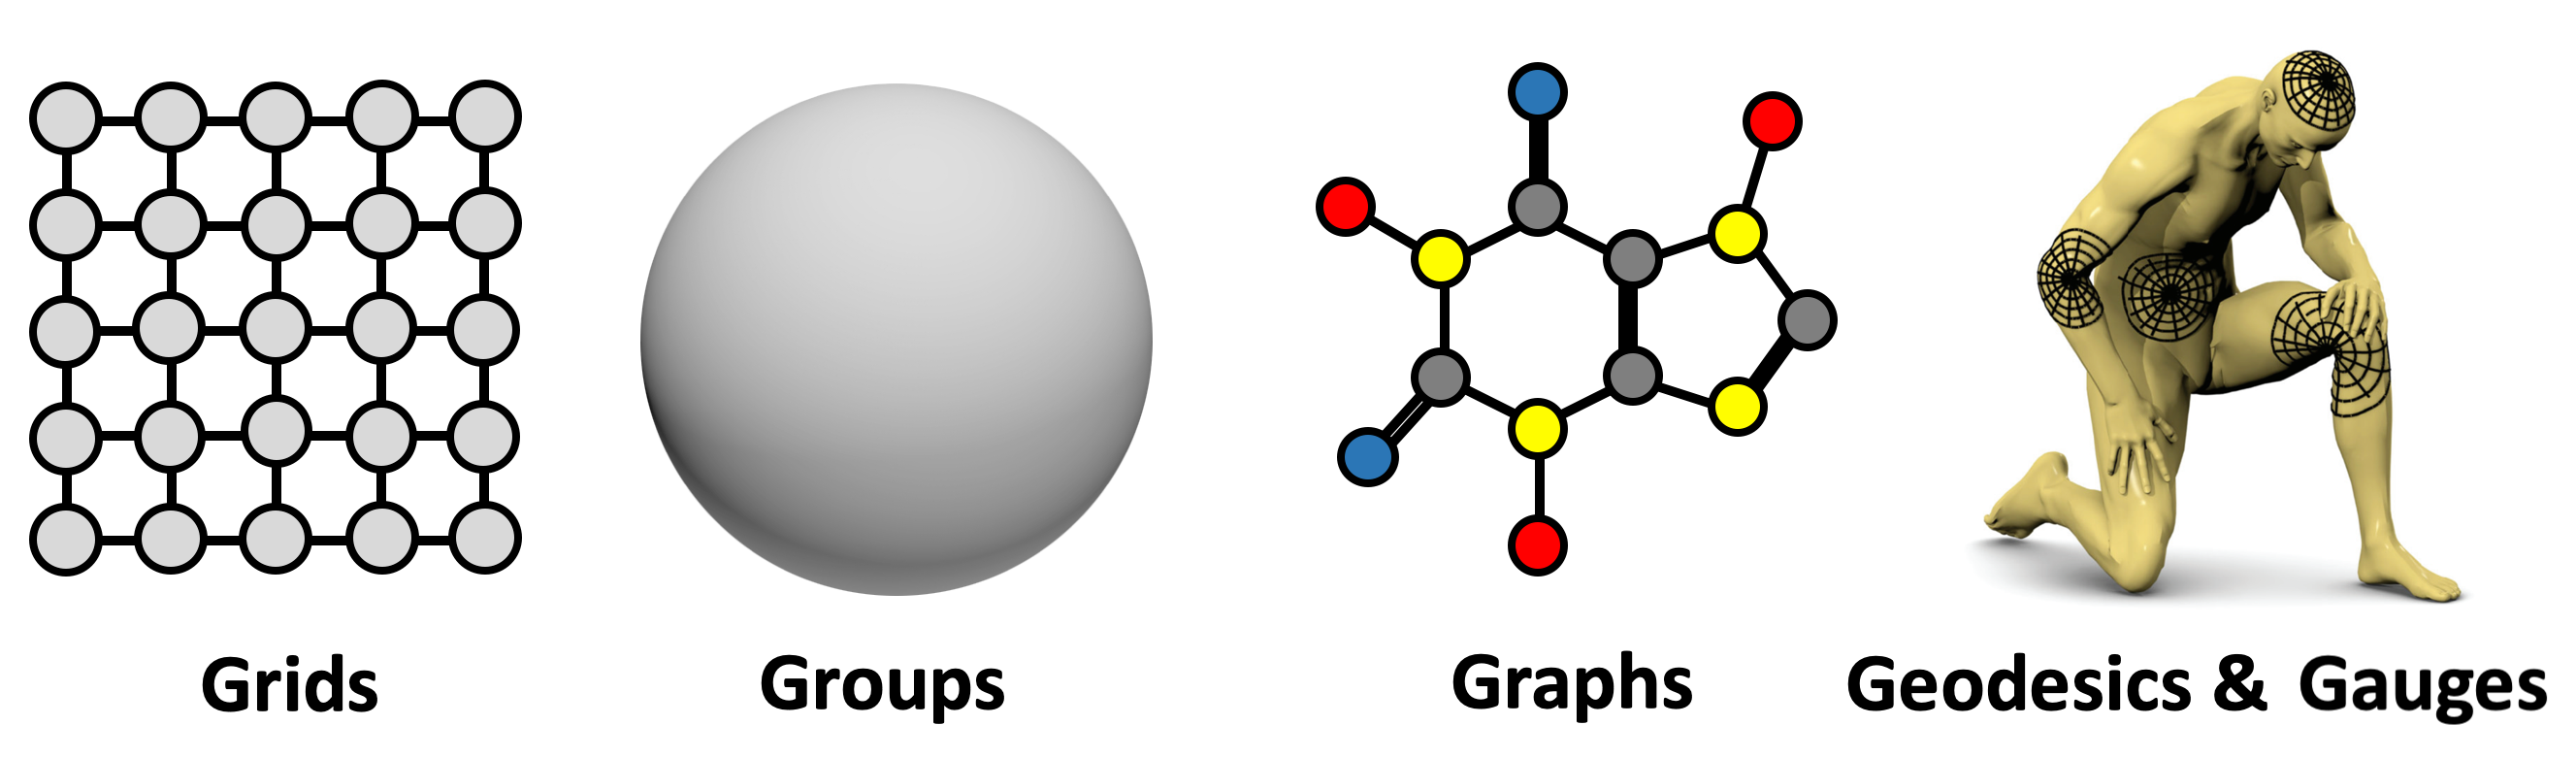
\includegraphics[width=1\textwidth]{figures/5g.png}
    \caption{几何深度学习的 5G：网格，具有全局对称性的群与齐性空间，图，流形上的测地线与度量，以及规范（切空间或特征空间的标架）。}
    \label{fig:4g}
\end{figure}





\subsection{图与集合}\label{sec:proto-graphs}

%\joan{This is a very nice intro. 
%Just one comment: it would be great to use the transition from sets to graphs to reinforce the scale aspect mentioned in the previous sections. Sets cannot be coarsened in non-trivial ways, while graphs can. 

%Another more general aspect that we need to nail in this section that clearly separates the graph treatment from, say the grid treatment: the domain varies with the input and thus becomes `part' of the input. I think again the transition from set to graph is useful here. The set is always the same geometric object modulo the change in size. The graph provides a new input to the system (as you say, via et its adjacency). 
%}





%\michael{\bf [MB: I took the liberty to rewrite this section making it less detailed and more `conversational' like the style of the previous sections in the Introduction chapter, anticipating that Chapter on graphs to be more rigorous.]}


%\joan{Joan: 
% Great detail and everything important seems to be here already. Two remarks:
% \begin{itemize}
%     \item I would frontload the section a bit more, explaining that we will first describe the domain, and then explain how the geometric priors and the blueprint are expressed.
%     \item Currently, this section re-derives the definitions of invariance/equivariance described previously, as well as the blueprint. I think it can be made shorter and more coherent to simply describe the two forms of group representation arising here (one for sets, and the other for graphs, where adjacency is also present), as well as the metric induced in the graph that is used to define local operators. 
%     \item In other words, I think these sections should derive the class of local linear equivariants for each symmetry group under consideration. In this section of sets and graphs, we should explain the two classes that arise (cf Maron et al.). 
%     \item The notation needs to be unified with the previous sections. 
%     
% \end{itemize}
%}

%\michael{MB: Agree in principle but we should not fall into the Bourbaki extreme. I suggest keep domain-specific notation to use familiar concepts and relate them to blueprint on the high level rather than in detail.

%I suggest to remove reference to particular models and talk about general concepts here. 
%}

在从社会学到粒子物理学的多个科学分支中，图都被用于对关系与交互系统建模。从我们的视角来看，图产生了一类由置换群刻画的基本不变性。
此外，我们关心的其他对象，如网格与集合，也可以作为图的特例得到。
%
%since graphs exhibit less restrictive geometries and invariances, they invite for the most flexible class of architectures---the \emph{Graph Neural Networks} (GNN). As we will see, all of the neural architectures we will study in this book can be understood as a special case of the GNN, with injected additional geometric constraints and invariances.


%the {\em symmetric group}), a . 


{\em 图} $\gG = (\gV, \gE)$ 由{\em 节点}\marginnote{视应用领域而定，节点也称为\emph{顶点}，边也常称为\emph{链接}或\emph{关系}。本文将交替使用这些术语。}集合 $\gV$ 以及节点对之间的{\em 边}集合 $\gE \subseteq \gV\times \gV$ 构成。为便于下文讨论，我们进一步假设节点配备 $s$ 维{\em 节点特征}，
记为 $\mathbf{x}_u$，其中 $u \in \gV$。
%
社交网络或许是最常研究的图实例之一，其中节点表示用户，边对应用户间的好友关系，节点特征则刻画年龄、头像等用户属性。通常也可以为边或整张图配备特征；\marginnote{
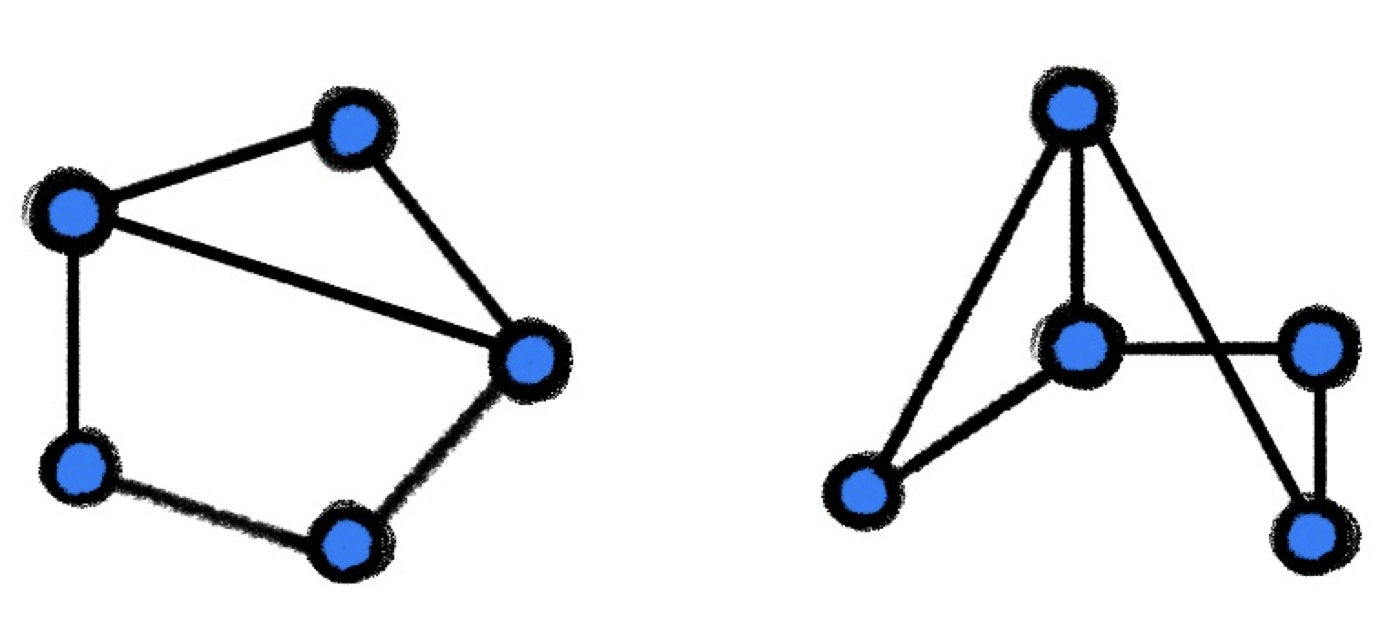
\includegraphics[width=0.8\linewidth]{figures/mn_isomorphic.png}
{\em 同构}是两个图之间保持边的双射。这里所示的两个同构图除节点顺序外完全相同。
}但这不会改变本节的主要结论，因此将留待后续工作讨论。


图的关键结构性质在于，通常不假设 $\gV$ 中的节点按任何特定顺序给出，因此在图上执行的任何运算都不应依赖节点排序。作用于图的函数所应满足的性质因而是{\em 置换不变性}；它意味着对于任意两个\emph{同构}图，这些函数的输出完全相同。
%
%
%This is clearly a 
我们可以把它视为蓝图的一种
特殊设定，其中域为 $\Omega = \mathcal{G}$，而空间 $\mathcal{X}(\mathcal{G},\mathbb{R}^d)$ 由 $d$ 维逐节点信号构成。
%
我们所考虑的对称性由\emph{置换群} $\mathfrak{G} = \Sigma_n$ 给出，其元素是节点索引集合 $\{1,\hdots, n\}$ 的所有可能排序。

%\michael{Harmonize notation: do we use $s$ or $d$ for dimension of features? } \joan{I am making a pass, using $s$ for feature dimension}\michael{we always used $d$, changing}

%In the language of the previous sections:\marginnote{However, we will almost always omit such notation for graphs, as they are assumed to be \emph{discrete} collections of nodes; hence, the language of linear algebra will admit higher notational simplicity.} for graphs we consider the input space to be defined on the domain  $\Omega = \mathcal{V}$, with the input space $\mathcal{X}(\mathcal{G}) = \{x : \mathcal{V}\rightarrow\mathbb{R}^s\}$ consisting of functions that attach node feature vectors to every node; $x(v) = \vec{x}_v$.
%\joan{Notation-wise: align with previous section $\Omega$ for domain, $\gX$ for signals over the domain} \michael{We use $x$ for signals, but $\Omega$ must be specific. }



%
%Accordingly, we focus on the permutation group actions $\frak{g}\in\frak{G}$ that permute the node ordering by applying such a matrix: $\frak{g}.{\bf X} = {\bf P}{\bf X}$. %


%$$ (where $n$ is the number of nodes).

%\begin{equation}
%    {\bf P}_{(2, 4, 1, 3)}{\bf X} =
%    \left[
%    \begin{array}{cccc}
%        0 & 1 & 0 & 0\\
%        0 & 0 & 0 & 1\\
%        1 & 0 & 0 & 0\\
%        0 & 0 & 1 & 0
%    \end{array}\right]\left[
%  \begin{array}{ccc}
%    \horzbar & \mathbf{x}_1 & \horzbar \\
%    \horzbar & \mathbf{x}_2 & \horzbar \\
%      \horzbar        &   \mathbf{x}_3  &    \horzbar       \\
%    \horzbar & \mathbf{x}_4 & \horzbar
%  \end{array}\right] = \left[\begin{array}{ccc}
%   \horzbar & \mathbf{x}_2 & \horzbar \\
%    \horzbar & \mathbf{x}_4 & \horzbar \\
 %     \horzbar        &   \mathbf{x}_1  &    \horzbar       \\
%    \horzbar & \mathbf{x}_3 & \horzbar
%  \end{array}\right]
%\end{equation}




%The first kind of object we will be studying is that of the \emph{graph}, which corresponds to the mother of all finite symmetry groups: the group of permutations. For the purposes of this chapter, we will define graphs as $G=(V, E)$, where $V$ is the set of \emph{nodes} and $E\subseteq V\times V$ is a set of \emph{edges} between pairs of nodes. For a commonly-studied example, social networks can be readily represented as graphs where nodes correspond to users, and edges correspond to the friendship links between them. 

%For now, we will assume that the graph's nodes are endowed with \emph{node features}, represented by $\mathcal{X} = \left\{\mathbf{x}_1, \mathbf{x}_2, \dots, \mathbf{x}_{|V|}\right\}$, where $\mathbf{x}_i\in\mathbb{R}^k$ are the features of node $i\in V$. In the social network analogy, these features could correspond to (some encoding of) the user's biography, interests or profile picture. Additional featurizations are possible, e.g. having features on the edges or entire graphs, but we will omit them for simplicity for now. 

%Compared with the subsequent objects, graphs exhibit less restrictive geometries and invariances, and hence invite for the most flexible class of architectures---the \emph{Graph Neural Networks} (GNN). Indeed, all of the neural architectures we will study can be understood as a special case of the GNN, with injected additional geometric constraints and invariances.

%The key structural property of graphs is that the nodes in $V$ are usually not assumed to be provided in any particular order, and thus any operations performed on graphs should not depend on the ordering of nodes. This desirable property that operations should satisfy is {\em permutation invariance}, and it implies that for any two \emph{isomorphic} graphs,\footnote{Isomorphism is an edge-preserving bijection between two graphs. Two isomorphic graphs are identical up to reordering of their nodes. } the outcomes of these operations are identical. 


首先在\emph{集合}上说明置换不变性的概念；集合是没有边的图的特例（即 $\gE=\emptyset$）。
%
将节点特征按行堆叠为 $n\times d$ 矩阵
 $\mathbf{X} = (\mathbf{x}_1, \hdots, \mathbf{x}_n)^\top$，实际上便指定了节点的一种排序。
 %
置换 $\mathfrak{g}\in\Sigma_n$ 在节点集合上的作用相当于重新排列 $\mathbf{X}$ 的各行；这一作用可以表示为一个 $n\times n$ {\em 置换矩阵} $\rho(\mathfrak{g}) = \mathbf{P}$，\marginnote{这样的置换恰有 $n!$ 个，因此 $\Sigma_n$ 即使在 $n$ 不大时也是一个非常大的群。}其中每行每列恰有一个 $1$，其余元素均为零。



%  We may obtain a different ordering by applying an appropriate permutation matrix  $\mathbf{P}$,\marginnote{There are exactly $n!$ such permutations. } where each row and column contains exactly one $1$ and all the other entries are zeros. Accordingly, we focus on the permutation group actions $\frak{g}\in\frak{G}$ that permute the node ordering by applying such a matrix: $\frak{g}.{\bf X} = {\bf P}{\bf X}$. %
 
 %\begin{equation}
 %    a(\vec{x}, \vec{y}) = \left<\vec{W}\vec{x}, \vec{U}\vec{y}\right> \qquad a(\vec{x}, \vec{y}) = \vec{a}^\top({\bf Wx} + {\bf Uy})
 %\end{equation}
 
 %\begin{align*}
 %    {\bf x}^\top{\bf L}{\bf x} &= \frac{1}{2}\sum_{u\in\mathcal{V}}\sum_{v\in\mathcal{V}} a_{uv}(x_u - x_v)^2\\ &= \sum_{(u, v)\in\mathcal{E}} (x_u - x_v)^2
 %\end{align*}

 
 %, ${\bf P}\in\mathbb{R}^{|V|\times|V|}$, to ${\bf X}$. 
 


%Let ${\bf X}\in\mathbb{R}^{|V|\times k}$ be a \emph{node feature matrix} which is obtained by stacking $\mathbf{x}_i$ in a particular order. This effectively specifies one \emph{ordering} of this set of node features; we may obtain any different order by applying an appropriate permutation matrix, ${\bf P}\in\mathbb{R}^{|V|\times|V|}$, to ${\bf X}$. 
若作用于该集合的函数 $f$ 对任意此类置换矩阵 ${\bf P}$ 都满足 $f({\bf P}{\bf X}) = f({\bf X})$，则称其具有\emph{置换不变性}。一个简单的此类函数是
%, exploited by the Deep Sets model \citep{zaheer2017deep}, is
\begin{equation}
\label{eq:basicinv}
    f({\bf X}) = \phi\left(\sum_{u\in \gV} \psi\left(\mathbf{ x}_u\right)\right)~,
\end{equation}
其中，函数 $\psi$ 独立地作用于每个节点的特征，$\phi$ 则作用于这些输出的\emph{求和聚合}结果。由于求和与输入的给定顺序无关，这类函数对节点集合的置换保持不变，因而无论如何置换节点，都保证返回相同的输出。

%\michael{Notation: should we use $\mathbf{f}(\mathbf{X})$ since the output can be a vector?}
%\petar{I would tend to stick with the $f$ notation}

 
%node features in $\mathcal{X}$ are permuted.



上述函数给出“全局”的图级输出，但很多时候，我们更关心以逐节点方式“局部”作用的函数。
%return more fine-grained information. 
例如，我们可能希望应用某个函数来\emph{更新}每个节点的特征，从而得到一组\emph{潜在}节点特征。
%, $\mathbf{h}_1, \hdots, \mathbf{h}_n$. 
%$\mathcal{H}=\left\{\mathbf{h}_1, \mathbf{h}_2, \dots, \mathbf{h}_{|V|}\right\}$.
%
%Strictly speaking, 
如果把这些潜在特征堆叠为矩阵 $\mathbf{H} = \mathbf{F}({\bf X})$\marginnote{我们对函数使用粗体记号 $\mathbf{F}(\mathbf{X})$，以强调它输出逐节点向量特征，因而是矩阵值函数。}，所得函数便不再具有置换不变性：${\bf H}$ 的行顺序应与 ${\bf X}$ 的行顺序\emph{绑定}，这样才能知道哪个输出节点特征对应哪个输入节点。我们转而需要更细致的{\em 置换等变性}概念：一旦“选定”输入的一种置换，该置换就会一致地作用于所得对象。
%
形式化地说，若 $\mathbf{F}(\mathbf{X})$ 对任意置换矩阵 ${\bf P}$ 都满足 $\mathbf{F}({\bf P}{\bf X}) = {\bf P}\mathbf{F}({\bf X})$，则它是\emph{置换等变}函数。一个共享的逐节点线性变换
\begin{equation}
    \mathbf{F}_{\mathbf\Theta}({\bf X}) = {\bf X}{\mathbf \Theta}
    %\qquad \text{, i.e.,} \qquad {\vec h}_i = {\mathbf\Theta}^T\mathbf{x}_i
\end{equation}
由权重矩阵 $\mathbf\Theta\in\mathbb{R}^{d\times d'}$ 指定，是构造此类置换等变函数的一种方式；在我们的例子中，它产生如下形式的
潜在特征：
$\mathbf{h}_u = \boldsymbol{\Theta}^\top\mathbf{x}_u$.
%\joan{This is very clear and nicely explained, but it is a particular case of the group equivariance discussion from previous section. I would add a pointer at the beginning or the end of this paragraph to tie things together. Upps just saw the following paragraph, nevermind. }

%\michael{Notation: do we use $h$ or $y$ for output?}
%\petar{$h$ for what comes out of an equivariant layer; the assumption is that we can stack more than one, or even attach invariant tail, to get a desirable $y$ (which should maybe be reserved for downstream task outputs?).}


%In fact, the construction from Equation (\ref{eq:basicinv}) arises naturally from the GDL blueprint. 
这一构造自然地源自几何深度学习蓝图。
我们可以首先尝试刻画{\em 线性等变映射}（形如 $\mathbf{F} {\bf P X} = \bf{P} \mathbf{FX}$ 的函数）；容易验证，
任意此类映射都可以写成两个\emph{生成元}的线性组合：恒等映射 $\mathbf{F}_1 \mathbf{X} = {\bf X}$ 与平均映射 ${\mathbf{F}_2 \mathbf{X}}= \frac{1}{n}\boldsymbol{1}\boldsymbol{1}^\top \mathbf{X} = \frac{1}{n} \sum_{u=1}^n {\bf x}_u$。正如第~\ref{sec:deepset} 节将描述的，流行的 Deep Sets \citep{zaheer2017deep} 架构恰好遵循这一蓝图。
%\joan{Remark to avoid confusion that $\mathbf{X}$ here should be understood as a vector, not a matrix}


% TODO: explain relation to representations & equivariance as explained in previous section.
% Invariant features correspond to a trivial representation
% Node features correspond to rho(P) = P
% Edge features / adjacency matrix corresponds to rho(P) = P tensor P.


现在可以把置换不变性与等变性的概念从集合推广到图。
%
在一般设定 $\gE\neq\emptyset$ 下，图的连通性可由如下定义的 $n\times n$ {\em 邻接矩阵} $\mathbf{A}$ 表示，\marginnote{当图为{\em 无向图}时，即 $(u,v) \in \gE$ 当且仅当 $(v,u) \in \gE$，邻接矩阵是{\em 对称的}：$\mathbf{A}= \mathbf{A}^\top$。}
\begin{equation}
    a_{uv} = \begin{cases}
    1 & (u, v)\in \gE\\
    0 & \text{otherwise}.
    \end{cases}
\end{equation}
%
注意，此时邻接矩阵 $\mathbf{A}$ 与特征矩阵 $\mathbf{X}$ 是“同步的”，即 $a_{uv}$ 指定了由第 $u$ 行和第 $v$ 行所描述节点之间的邻接信息，而这些行属于 $\mathbf{X}$。因此，把置换矩阵 $\mathbf{P}$ 施加于节点特征 $\mathbf{X}$，就必然也要对 $\mathbf{A}$ 的行和列施加置换，得到 $\mathbf{P}\mathbf{A}\mathbf{P}^\top$。\marginnote{$\mathbf{P}\mathbf{A}\mathbf{P}^\top$ 是 $\Sigma_n$ 作用于矩阵的表示。}
%
%
若（图级函数）$f$ 满足下式，则称其具有\emph{置换不变性}：
\begin{equation}
f({\bf PX}, {\bf PAP}^\top) = f({\bf X}, {\bf A})\marginnote{As a way to emphasise the fact that our functions operating over graphs now need to take into account the adjacency information, we use the notation $f({\bf X}, {\bf A})$.}
\end{equation}
若（逐节点函数）$\mathbf{F}$ 满足下式，则称其具有\emph{置换等变性}：
\begin{equation}
\label{eq:permequivgraph}
\mathbf{F}({\bf PX}, {\bf PAP}^\top) = {\bf P}\mathbf{F}({\bf X}, {\bf A})
\end{equation}
其中 ${\bf P}$ 为任意置换矩阵。
%
%
%\taco{Taco: should we relate this to the blueprint? We can mention here that $PX$ and $PAP^T$ are examples of representations of the permutation group. We can then go on to say that the graph structure tells us which nodes are close in a certain sense, and that most graph nets exploit this, leading into the next paragraph.}\michael{I do say above that $\rho(\fg)=P$}
%
%Armed with the concepts of permutation invariance and equivariance, we can consider a generic graph connectivity setup, where $E\neq\emptyset$. One typical way to represent this adjacency information in a compact form is the \emph{adjacency matrix}, ${\bf A}\in\mathbb{R}^{|V|\times|V|}$, which is in the simplest case (of an unweighted and undirected graph), a binary and symmetric matrix; that is:
%\begin{equation}
%    {\bf A}_{ij} = {\bf A}_{ji} = \begin{cases}
%    1 & (i, j)\in E\\
%    0 & \text{otherwise}
%    \end{cases}
%\end{equation}
%
%
%We can now generalise the notions of permutation invariance and equivariance from sets to graphs. We note that the order of the rows and columns in ${\bf A}$ is constrained to respect the order of the rows of ${\bf X}$---that is, ${\bf A}_{ij}$ specifies the adjacency information between the nodes described by the $i$-th and $j$-th row of ${\bf X}$. Then, applying a permutation matrix ${\bf P}$ to the nodes in ${\bf X}$ automatically implies applying it to ${\bf A}$'s rows and columns, yielding ${\bf P}{\bf A}{\bf P}^T$. 


%Following again the Geometric Deep Learning blueprint, 
这里同样可以先刻画线性等变函数。\marginnote{这对应于{\em Bell 数} $B_4$，它计算对含 $4$ 个元素的集合进行划分的方式数；此处这四个元素是为作用于邻接矩阵的线性映射编制索引的四个指标 $(u,v), (u',v')$。%\cite{maron2018invariant}.
}  
正如 \cite{maron2018invariant} 所观察到的，任何满足式（\ref{eq:permequivgraph}）的线性 $\mathbf{F}$ 都可以表示为
十五个线性生成元的线性组合；值得注意的是，这一生成元族与 $n$ {\em 无关}。
%
%
%
在这些生成元中，我们的蓝图尤其提倡同时具有{\em 局部性}的生成元，即
节点 $u$ 上的输出直接依赖图中与其相邻的节点。通过定义一个节点与另一个节点相邻的含义，可以在模型构造中显式形式化这一约束。



节点 $u$ 的（无向）{\em 邻域}有时也称为 {\em 1-hop}，定义如下：\marginnote{
%Our definition of neighbourhood does not account for directed edges. 
通常也把节点 $u$ 本身包含在其邻域中。}
\begin{equation}
    \mathcal{N}_u = \{ v : (u,v) \in \gE \,\mathrm{or}\, (v,u) \in \gE \}
    %\left\{j\ |\ i=j\vee {\bf A}_{ij} = 1\right\}
\end{equation}
%
并把{\em 邻域特征}定义为多重集
%
\begin{equation}
    \mathbf{X}_{\mathcal{N}_u} = \ldblbrace \mathbf{x}_v : v\in\mathcal{N}_u \rdblbrace.
\marginnote{A {\em multiset}, denoted $\ldblbrace \, \dots \, \rdblbrace$, is a set where the same element can appear more than once. This is the case here because the features of different nodes can be equal.}
\end{equation}
%%
对 1-hop 邻域进行运算与蓝图的\emph{局部性}方面非常契合：具体而言，把图上的度量定义为沿 $\mathcal{E}$ 中边计算的节点间\emph{最短路径距离}。% \michael{I suggest we get rid of this, since we never talked about metrics in a rigorous way. } \petar{There seems to still be a discussion of a metric when defining locality in the blueprint---this is what I was referring to. I think it's fine as-is, but wouldn't mind removing it.} \joan{I think mentioning it qualitatively like this is fine, it conveys an important message}
%Processing 1-hop neighbourhoods over graphs exactly corresponds with defining our metric over graphs, $g$, as the \emph{shortest path distance} between nodes using edges in $\mathcal{E}$, and setting $\delta = 1$.

%This also closely aligns with the \emph{locality} condition of the main building block of our geometric deep learning blueprint. Processing 1-hop neighbourhoods over graphs exactly corresponds with defining our metric over graphs, $g$, as the \emph{shortest path distance} between nodes using edges in $\mathcal{E}$, and setting $\delta = 1$.

%
因此，GDL 蓝图给出了在图上构造置换等变函数的一般方案：指定一个作用于节点及其邻域特征的\emph{局部}函数 $\phi$，即 $\phi(\mathbf{x}_u, \mathbf{X}_{\mathcal{N}_u})$。随后，可以构造置换等变函数 $\mathbf{F}$，方法是把 $\phi$ 分别应用于每个节点的邻域（见图~\ref{fig:gc_gdl}）：
\begin{equation}
    \mathbf{F}({\bf X}, {\bf A}) =
\left[
  \begin{array}{ccc}
    \horzbar & \phi(\mathbf{x}_1, \mathbf{X}_{\mathcal{N}_1}) & \horzbar \\
    \horzbar & \phi(\mathbf{x}_2, \mathbf{X}_{\mathcal{N}_2}) & \horzbar \\
             & \vdots    &          \\
    \horzbar & \phi(\mathbf{x}_n, \mathbf{X}_{\mathcal{N}_n}) & \horzbar
  \end{array}
\right]
\label{eq:graph_equivariant}
\end{equation}
由于 $\mathbf{F}$ 是通过在每个节点处局部应用共享函数 $\phi$ 构造的，其置换等变性取决于 $\phi$ 的输出是否独立于 $\mathcal{N}_u$ 中节点的排序。因此，只要把 $\phi$ 构造为置换不变函数，就能满足这一性质。
%
正如后续工作将说明的，$\phi$ 的选择对这类方案的表达能力起着关键作用。当 $\phi$ 为单射时，它等价于{\em Weisfeiler-Lehman 图同构检验}的一步；这是图论中的经典算法，通过迭代颜色细化过程给出两个图同构的必要条件。


%\michael{ADD: geometric stability of graph filters}

%We conclude our introduction with a discussion on how to generally construct useful functions over graphs that are permutation equivariant. A function over graphs is likely to be useful if it directly exploits the structure present in ${\bf A}$---that is, if outputs on node $i$ directly depend on its \emph{neighbouring} nodes in the graph (e.g. the non-zero entries of $\mathbf{a}_i$ and $\mathbf{a}_i^T$).

%From this concept, we can define a \emph{neighbourhood} of node $i$ in the graph, commonly denoted as $\mathcal{N}_i$, to include all first-order neighbours of $i$, often including $i$ itself:
%\begin{equation}
%    \mathcal{N}_i = \left\{j\ |\ i=j\vee {\bf A}_{ij} = 1\right\}
%\end{equation}
%Accordingly, we can define the set of \emph{neighbourhood features} of $i$, $\mathbf{X}_{\mathcal{N}_i}\in\mathcal{P}(\mathbb{R}^k)$:
%\begin{equation}
%    \mathbf{X}_{\mathcal{N}_i} = \left\{\mathbf{x}_j\ |\ j\in\mathcal{N}_i\right\}
%\end{equation}
\begin{figure}
    \centering
    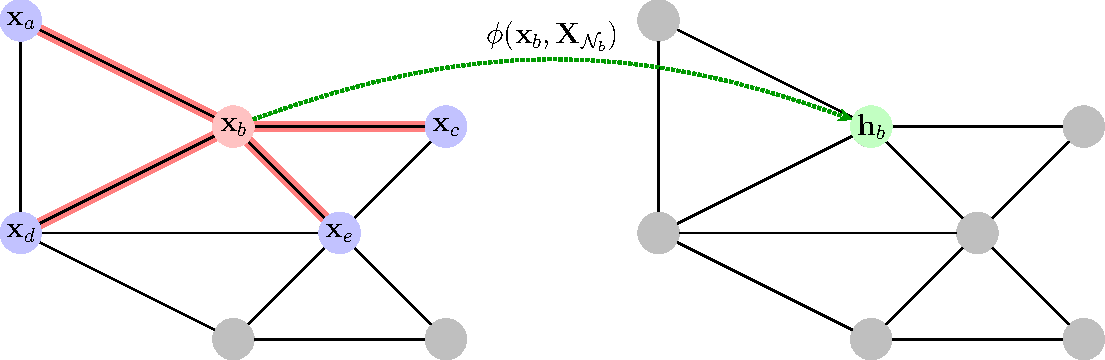
\includegraphics[width=\linewidth]{figures/GC_GDL.pdf}
    \caption{通过对每个邻域应用置换不变函数 $\phi$，在图上构造置换等变函数的示意图。在此例中，$\phi$ 作用于特征 $\mathbf{x}_b$（对应节点 $b$），以及它的邻域特征多重集 $\mathbf{X}_{\mathcal{N}_b} = \ldblbrace\mathbf{x}_a, \mathbf{x}_b, \mathbf{x}_c, \mathbf{x}_d, \mathbf{x}_e\rdblbrace$。以这种方式把 $\phi$ 应用于每个节点的邻域，即可得到所生成潜在特征矩阵 $\mathbf{H}=\mathbf{F}(\mathbf{X}, \mathbf{A})$ 的各行。}
    \label{fig:gc_gdl}
\end{figure}%
%\michael{\bf [MB: shall we use the notation of multisets here?]}


%The general concept of constructing {\em permutation equivariant} functions operating over graphs as shared {\em permutation invariant} functions operating over local neighbourhoods appears to be very powerful and underlies the design of most Graph Neural Networks. Under various guises, this local function $g$ can be referred to as ``diffusion'', ``propagation'', or ``message passing''. 
%
%If we are interested in a graph-level output, a common recipe is to construct the latent node features using a {\em permutation equivariant} function $f$, followed by a {\em permutation invariant} function $h$ over the entries of $f({\bf X}, {\bf A})$ to obtain an ordering-independent output. In this context, the function $h$ is often referred to as ``readout'' or ``global pooling''.

%Motivation: examples from 
%- Images, Text, Speech. 
%- Social Networks
%- Physical Sciences
%- Chemistry and medicine
%- 3D Computer vision and Graphics


%Finally, 
还应注意，在这个例子中，定义在集合上的函数与定义在更一般图上的函数之间的区别在于：后一种情形需要显式考虑域的结构。
%
因此，图的特殊之处在于域成为机器学习问题中{\em 输入的一部分}；而在处理集合和网格（两者都是图的特例）时，我们可以只指定特征，并假定域{\em 固定}。
%
这一区别将在后文讨论中反复出现。
%
因此，几何稳定性（对域形变的不变性）概念在大多数图学习问题中都至关重要。由我们的构造直接可知，置换不变函数和置换等变函数在同构（拓扑等价）图上产生相同输出。这些结果可以推广到近似同构图，且已有若干关于图扰动下稳定性的结果 \citep{levie2018cayleynets}。在讨论流形时，我们将回到这一要点，并以流形为载体更详细地研究此类不变性。


其次，与集合不同，图和网格由于具有附加结构，可以进行非平凡粗化\marginnote{更准确地说，仅假定集合结构时无法定义非平凡粗化。已有一些成熟方法可以从无序集合推断拓扑结构，而这些方法能够支持非平凡粗化。}，由此产生多种池化操作。
%These will also be covered within Chapter \ref{ch:graphs}. 
%
%Finally, 



\subsection{网格与 Euclidean 空间}
\label{sec:grids_euclidean}

%\joan{Joan: Good section; perhaps we could shrink a bit by removing the repetitive parts between blueprint, discrete and then continuous case. Also further highlight the fundamental differences between grids and graphs in terms of group representation (permutation group vs translation group, one-parameter group in one case), and geometry (homogeneous vs non-homogeneous): consequences in terms of global orientation, etc. 
%}
%\michael{This more naturally comes after the Groups section, was a natural transition to manifolds which are non-homogeneous}

%images, CNNs, RNNs

我们考虑的第二类对象是网格。
%
可以说，深度学习对计算机视觉、自然语言处理和语音识别的影响尤为显著。这些应用都共享一个%an essential
几何共同点：底层网格结构。
%translation invariance/equivariance, alongside scale separation. 
%
如前所述，网格是具有特殊邻接关系的图的特例。然而，由于网格中的节点顺序固定，定义在网格信号上的机器学习模型不再需要考虑置换不变性，并且具有更强的几何先验：平移不变性。
%can be designed to leverage the translation invariance prior. 

%This gives rise to powerful and efficient deep learning architectures---{\em Convolutional Neural Networks} (CNNs). 



\paragraph{循环矩阵与卷积}
下面更详细地讨论这一点。
为简单起见，假设采用周期边界条件，可以把一维网格视为{\em 环图}\marginnote{
    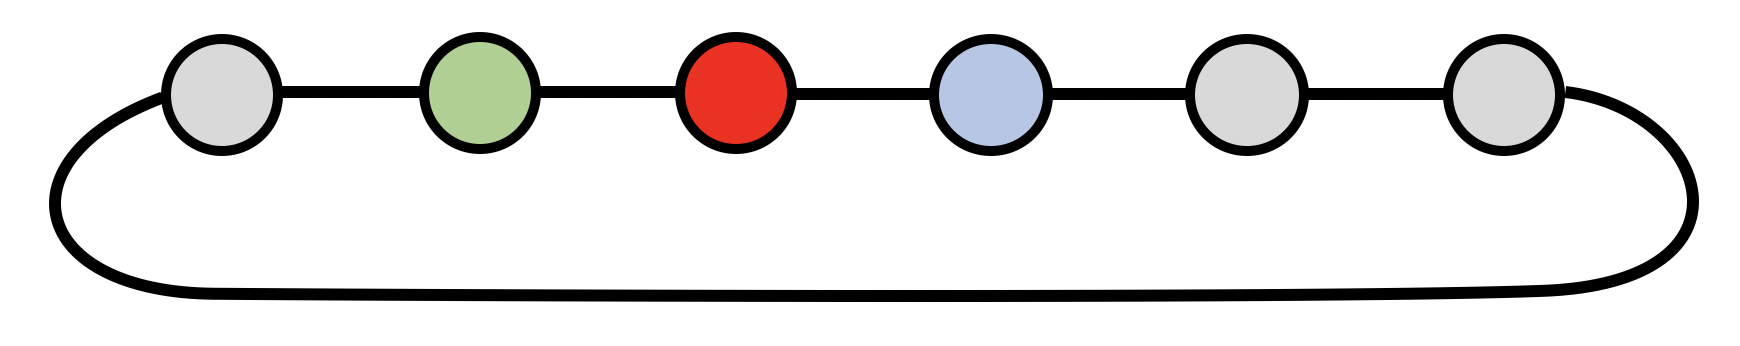
\includegraphics[width=0.9\linewidth]{figures/grid.png}
}，其节点编号为 $0, 1,\hdots, n-1$，并按 $n$ 取模（为简化记号，下文将省略模数），而且
邻接矩阵的元素满足 $a_{u,u+1 \, \mathrm{mod} \, n} = 1$，其余元素为零。它与此前讨论的一般图情形存在两个主要区别。
%
第一，每个节点 $u$ 都与其邻居 $u-1$ 和 $u+1$ 具有相同的连接方式，因而在结构上无法与其他节点区分。
%in terms of group theory, we say that the grid is a homogeneous space. 
\marginnote{正如后文将看到的，这使网格成为齐性空间。
  %  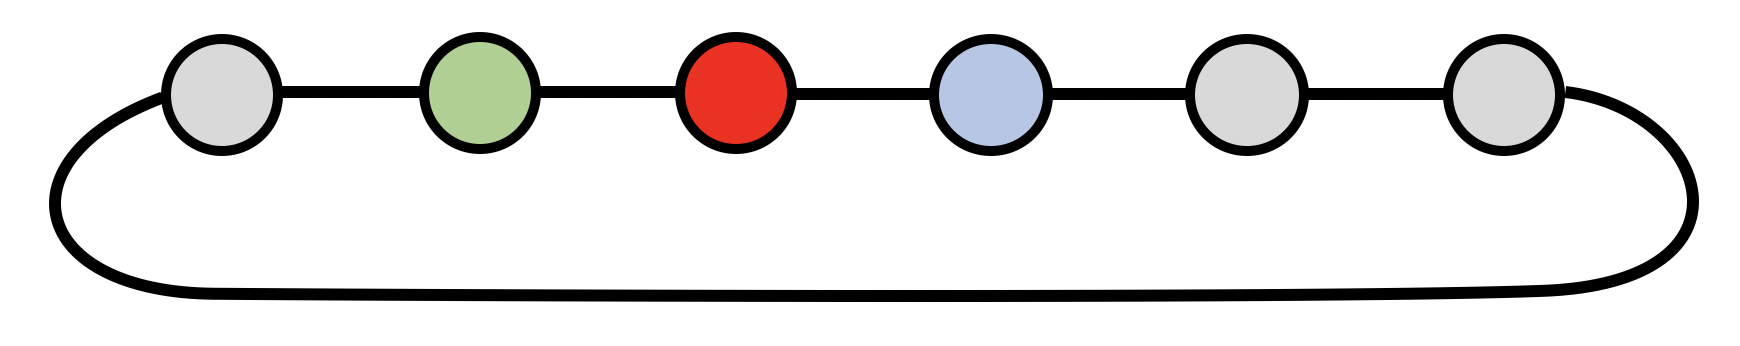
\includegraphics[width=1\linewidth]{figures/grid.png}
}
%
第二，也是更重要的一点，由于网格节点具有固定顺序，其{\em 邻居}也具有固定顺序：可以把 $u-1$ 称为“左邻居”，把 $u+1 $ 称为“右邻居”。
%
如果采用之前设计等变函数 $\mathbf{F}$ 的方案，并使用局部聚合函数 $\phi$，那么现在网格的每个节点上都有 $\mathbf{f}(\mathbf{x}_u) = \phi(\mathbf{x}_{u-1}, \mathbf{x}_{u}, \mathbf{x}_{u+1})$：$\phi$ 不再需要具有置换不变性。
%
%
对线性变换作特定选择 $\phi(\mathbf{x}_{u-1}, \mathbf{x}_{u}, \mathbf{x}_{u+1}) = \theta_{-1}\mathbf{x}_{u-1} + \theta_0 \mathbf{x}_{u} + \theta_1 \mathbf{x}_{u+1}$ 后，可以把 $\vec{F}(\mathbf{X})$ 写成矩阵乘积：
$$
\vec{F}(\mathbf{X}) = 
\left[
\begin{array}{ccccc}
\theta_0 & \theta_1  & & & \theta_{-1}\\
 \theta_{-1} & \theta_0 & \theta_1 & & \\
&  \ddots & \ddots & \ddots & \\
 &  & \theta_{-1} & \theta_0 & \theta_1\\
\theta_1 &  &  & \theta_{-1} & \theta_0

 \end{array}
  \right]
  %
\left[  
    \begin{array}{ccc}
    \horzbar & \mathbf{x}_0 & \horzbar \\
    \horzbar & \mathbf{x}_1 & \horzbar \\
             & \vdots    &          \\
    \horzbar & \mathbf{x}_{n-2} & \horzbar  \\           
    \horzbar & \mathbf{x}_{n-1} & \horzbar
  \end{array}
   \right]
$$
%
注意这种非常特殊的多对角结构：每条对角线上都重复同一个元素。在机器学习文献中，这有时称为“权重共享”。
%
%In machine learning literature, it is sometimes referred to as %``weight sharing'', a prominent feature of CNNs where the same %weights are applied at different positions in an image. 

%\michael{Notation: we denoted filters by $\theta$}

更一般地，给定向量 $\boldsymbol{\theta} = (\theta_0, \hdots, \theta_{n-1})$，{\em 循环矩阵}
$\mathbf{C}(\boldsymbol{\theta}) = (\theta_{u-v \, \mathrm{mod} \, n})$ 由向量 $\boldsymbol{\theta}$ 的循环移位版本依次排列得到。
%
循环矩阵与离散卷积等价，\marginnote{由于采用周期边界条件，这里是{\em 圆周卷积}或{\em 循环卷积}。在信号处理中，$\boldsymbol{\theta}$ 常称为“滤波器”；在 CNN 中，其系数是可学习的。}
%\taco{TODO: change this equation to a cross-correlation, and add a note saying that technically this is called a cc but we'll call it a conv.}
$$
(\mathbf{x} \star \boldsymbol{\theta})_u = \sum_{v=0}^{n-1}  x_{v \, \mathrm{mod}\, n} \,\, \theta_{u-v \, \mathrm{mod}\, n}
$$
%
因为有 $\mathbf{C}(\boldsymbol{\theta})\mathbf{x} = \mathbf{x} \star \boldsymbol{\theta}$。
%\petar{Should $i$ be replaced with $u$ in the equation above, given our blueprint? I did this in the CNN section.}
%
特定选择 $\boldsymbol{\theta}=(0,1,0,\hdots, 0)^\top$ 会产生一种特殊循环矩阵，它把向量向右移动一个位置。该矩阵称为（右）{\em 移位}或{\em 平移算子}，记为 $\mathbf{S}$。\marginnote{左移算子由 $\mathbf{S}^\top$ 给出。显然，先左移再右移（或反之）不会改变任何内容，这意味着 $\mathbf{S}$ 是{\em 正交的}：$\mathbf{S}^\top \mathbf{S} = \mathbf{S} \mathbf{S}^\top = \mathbf{I}$。}


%\michael{Notation: Replace $T$ by $S$}


%\michael{Naming: shift vs translation}


循环矩阵可以由其{\em 交换性}刻画：循环矩阵的乘积满足交换律，即
$\mathbf{C}(\boldsymbol{\theta}) \mathbf{C}(\boldsymbol{\eta}) = \mathbf{C}(\boldsymbol{\eta}) \mathbf{C}(\boldsymbol{\theta})$ 对任意 $\boldsymbol{\theta}$ 和 $\boldsymbol{\eta}$ 均成立。
%
由于移位是循环矩阵，便得到熟知的卷积算子{\em 平移等变性}或{\em 移位等变性}：
$$
\mathbf{S} \mathbf{C}(\boldsymbol{\theta}) \mathbf{x} = 
\mathbf{C}(\boldsymbol{\theta}) \mathbf{S} \mathbf{x}.
$$
%
这种交换性并不令人意外，因为底层对称群（平移群）是 Abel 群。
此外，反向结论似乎也成立，即
一个矩阵为循环矩阵，当且仅当它与移位算子可交换。
%
这又使我们能够把卷积{\em 定义}为平移等变的线性运算，并很好地展示了几何先验的力量以及几何 ML 的整体理念：卷积从平移对称性的第一性原理中自然产生。


注意，与集合和图上的情形不同，线性无关的移位等变函数（卷积）数量会随域的大小而\emph{增长}（因为循环矩阵的每条对角线都有一个自由度）。不过，尺度分离先验保证滤波器可以是{\em 局部的}，从而使每层仍具有相同的 $\Theta(1)$ 参数复杂度；在第~\ref{sec:cnnsec} 节讨论这些原则如何用于实现卷积神经网络架构时，我们将验证这一点。

%\joan{Link to GDL blueprint: 
%Convolutions also emerge as the essential device to build stable translation invariant representations, by querying the GDL blueprint. 
%Remark that, as opposed to the permutation group in sets and graphs, the number of linearly independent convolution maps \emph{grows} with the size of the domain (since we have one degree of freedom in each diagonal of a circulant matrix). However, the scale separation prior imposes only local filters, resulting in the same $\Theta(1)$-parameter complexity per layer, as we will verify in Section \ref{sec:cnnsec}.  }



\paragraph{离散 Fourier 变换的推导}
我们已经提到 Fourier 变换及其与卷积的联系：Fourier 变换能够对角化卷积运算，这一重要性质使信号处理中可以在频域通过 Fourier 变换的逐元素乘积执行卷积。
%
然而，教科书通常只陈述这一事实，很少解释 Fourier 变换究竟{\em 从何而来}，以及 Fourier 基为何如此{\em 特殊}。
%
这里将给出这一推导，再次说明对称性的基本原则何等根本。


为此，回顾线性\marginnote{还必须假设特征值互不相同，否则可能存在多个可能的对角化。我们所选的 $\mathbf{S}$ 满足这一假设。}代数中的一个事实：（可对角化）矩阵可以{\em 同时对角化}，当且仅当它们两两可交换。
%
换言之，所有循环矩阵都存在一个公共特征基，在该基下它们仅有特征值不同。
%
因此，可以任选一个循环矩阵并计算其特征向量——这些特征向量也必然是所有其他循环矩阵的特征向量。
%\taco{I think this is true only if all eigenvalues of this matrix are distinct. Take e.g. the identity matrix, which is circulant, and can be (re-)diagonalized by any orthogonal matrix. Using the shift operator is fine in this respect}\michael{The statement here is on the existence of a joint diagonalization. True, some circulant matrices have different bases diagonalizing them, but not all of them will diagonalize other matrices. }
选择移位算子最为方便，其特征向量恰好构成离散 Fourier 基。\marginnote{
$\mathbf{S}$ 正交但不对称，因此其特征向量相互正交，而特征值为复数（单位根）。
}
$$
\boldsymbol{\varphi}_k = \frac{1}{\sqrt{n}}\left (1, e^{ \frac{2\pi \mi k}{n}}, e^{ \frac{4\pi \mi k}{n} }, \hdots , e^{ \frac{2\pi \mi  (n-1)k}{n} }
\right)^\top, \hspace{5mm} k = 0, 1, \hdots, n-1,  
$$
%
可将这些向量排列为 $n\times n$ Fourier 矩阵 $\boldsymbol{\Phi} = (\boldsymbol{\varphi}_0, \hdots, \boldsymbol{\varphi}_{n-1})$。
% 
%
左乘 $\boldsymbol{\Phi}^*$\marginnote{注意，特征向量是复数，因此转置 $\boldsymbol{\Phi}$ 时需要取复共轭。}
得到离散 Fourier 变换（DFT），而左乘 $\boldsymbol{\Phi}$ 得到逆 DFT：
$$
\hat{x}_k = \frac{1}{\sqrt{n}}\sum_{u = 0}^{n-1}x_u e^{-\frac{2\pi \mi k u}{n} } \hspace{15mm}
%
{x}_u = \frac{1}{\sqrt{n}} \sum_{k = 0}^{n-1}\hat{x}_k e^{+\frac{2\pi \mi k u}{n} }.
$$

 
 
由于所有循环矩阵都可以同时对角化，\marginnote{
由于 Fourier 变换是正交矩阵（$\boldsymbol{\Phi}^* \boldsymbol{\Phi} = \mathbf{I}$），从几何上看，它相当于一次 $n$ 维旋转所对应的坐标系变换。在这一坐标系（“Fourier 域”）中，循环矩阵 $\mathbf{C}$ 的作用变为逐元素乘积。
}  
因而也都被 Fourier 变换对角化，
并且仅有特征值不同。由于循环矩阵 $\mathbf{C}(\boldsymbol{\theta})$ 的特征值就是滤波器的 Fourier 变换（例如见 \cite{bamieh2018discovering}），即 $\hat{\boldsymbol{\theta}} = \boldsymbol{\Phi}^* \boldsymbol{\theta}$，于是得到卷积定理：
$$
\mathbf{C}(\boldsymbol{\theta}) \mathbf{x} = \boldsymbol{\Phi}
\left[  
    \begin{array}{ccc}
    \hat{\theta}_0 &  &  \\
    & \ddots & \\
    & & \hat{\theta}_{n-1}
  \end{array}
   \right]\boldsymbol{\Phi}^*\mathbf{x}
   = \boldsymbol{\Phi} (\hat{\boldsymbol{\theta}} \odot \hat{\mathbf{x}} )
$$
%

由于 Fourier 矩阵 $\boldsymbol{\Phi}$ 具有特殊的代数结构，乘积 $\boldsymbol{\Phi}^\star \mathbf{x}$ 和 $\boldsymbol{\Phi} \mathbf{x}$ 可以利用快速 Fourier 变换（FFT）算法以 $\mathcal{O}(n \log n)$ 复杂度计算。这是频域滤波在信号处理中如此流行的原因之一；此外，滤波器通常直接在频域设计，因此从不显式计算其 Fourier 变换 $\hat{\boldsymbol{\theta}}$。


除了在教学上的价值之外，这里对 Fourier 变换
与卷积的推导还提供了一种把这些概念推广到图的方案。注意到环图的邻接矩阵恰好就是移位算子，便可以通过计算邻接矩阵的特征向量，构造图 Fourier 变换及卷积算子的类比（例如见 \cite{sandryhaila2013discrete}）。
%
早期通过类比 CNN 来发展图神经网络的尝试，有时称为“谱 GNN”，采用的正是这一蓝图。\marginnote{在图信号处理中，常用{\em 图 Laplacian} 的特征向量代替邻接矩阵来构造图 Fourier 变换，见 \cite{shuman2013emerging}。在网格上，这两个矩阵具有共同特征向量；但在图上，它们产生有所不同但彼此相关的构造。}
%
我们将在%Chapter~\ref{ch:graphs}
第~\ref{sec:manifolds}--\ref{sec:meshes} 节看到，
这一类比存在一些重要局限。
%
第一个局限源于网格是固定的，因此其上的所有信号都可以用同一个 Fourier 基表示。相比之下，在一般图上，Fourier 基依赖于图结构。因此，无法直接比较两个不同图上的 Fourier 变换——这一问题在机器学习任务中表现为缺乏泛化能力。
%
第二，多维网格由一维网格的张量积构造而成，并保留底层结构：Fourier 基元素及其对应频率（特征值）可以按多个维度组织。例如，在图像中，可以自然地讨论水平与垂直频率，滤波器也具有{\em 方向}概念。在图上，Fourier 域的结构是一维的，因为只能按对应频率的大小组织 Fourier 基函数。因此，图滤波器不感知方向，即具有{\em 各向同性}。



\paragraph{连续 Fourier 变换的推导}
为保证完整性，并为接下来的讨论作铺垫，我们在连续设定下重复上述分析。
与第~\ref{sec:scale_separation} 节类似，考虑定义在 $\Omega = \mathbb{R}$ 上的函数，以及平移算子 $(S_v f)(u) = f(u-v)$；该算子把 $f$ 平移某个位置 $v$。
 %
把 $S_v$ 施加到 Fourier 基函数 $\varphi_\xi(u) = e^{\mi \xi u}$ 上，利用指数运算的结合性得到
% \michael{Notation: same $\phi$ used to denote basis functions, filters, and local aggregators}
$$
S_v e^{\mi\xi u} = e^{\mi\xi (u-v)} = e^{-\mi\xi v} e^{\mi\xi u},
$$
即 $\varphi{u}_\xi(u)$ 是 $S_v$ 的复特征向量，对应复特征值 $e^{-\mi\xi v} $——这与离散设定下的情形完全一致。
由于 $S_v$ 是酉算子（即 $\| S_v x \|_p = \| x \|_p$ 对任意 $p$ 和 $x \in L_p(\R)$ 都成立），任意特征值 $\lambda$ 都必须满足 $|\lambda|=1$，这恰好对应于上面得到的特征值 $e^{-i\xi v}$。
此外，平移算子的谱是\emph{单谱}，即共享同一特征值的两个函数必然共线。事实上，假设 $S_v f = e^{-\mi \xi_0 v} f$ 对某个 $\xi_0$ 成立。对等式两边作 Fourier 变换，得到
$$\forall ~\xi~,~e^{-\mi \xi v} \hat{f}(\xi) = e^{-\mi \xi_0 v} \hat{f}(\xi)~,$$
这意味着 $\hat{f}(\xi)=0$ 对 $\xi \neq \xi_0$ 成立，因此 $f = \alpha \varphi_{\xi_0}$。

对于一般线性算子 $C$，若其具有平移等变性（$S_v C = C S_v$），则有
$$
S_v C e^{\mi\xi u} = C S_v e^{\mi\xi u} = e^{-\mi\xi v} C e^{\mi\xi u}, 
$$
这意味着 $C e^{\mi\xi u}$ 也是特征函数\marginnote{{\em 特征函数}与“特征向量”同义，用于指连续算子的特征向量。}，它属于 $S_v$，对应特征值 $e^{-\mi\xi v}$。
由谱的单谱性质可知 $C e^{\mi\xi u} = \beta \varphi_{\xi}(u)$；换言之，Fourier 基是所有平移等变算子的特征基。
%
因此，$C$ 在 Fourier 域中是\emph{对角的}，可以表示为 $C e^{\mi\xi u} = \hat{p}_{C}(\xi) e^{\mi\xi u}$，其中 $\hat{p}_{C}(\xi)$ 是作用于不同频率 $\xi$ 的{\em 传递函数}。
%
%
最后，对于任意函数 $x(u)$，由线性性可得
%\michael{Notation: use $\lambda$ in place of $\xi$ for frequency?}
%
\begin{eqnarray*}
(C x) (u) &=& C \int_{-\infty}^{+\infty} \hat{x}(\xi) e^{\mi \xi u} \mathrm{d}\xi = \int_{-\infty}^{+\infty} \hat{x}(\xi) \hat{p}_C(\xi) e^{\mi \xi u} \mathrm{d}\xi \\
&=& \int_{-\infty}^{+\infty} p_C(v) x(u-v) \mathrm{d}v~ = (x \star p_C)(u),\marginnote{The spectral characterisation of the translation group is a particular case of a more general result in Functional Analysis, the \emph{Stone's Theorem}, which derives an equivalent characterisation for any one-parameter unitary group.}
\end{eqnarray*}
%
其中 $p_C(u)$ 是 $\hat{p}_C(\xi)$ 的逆 Fourier 变换。因此，每个线性平移等变算子都是卷积。
% {\em quod erat demonstrandum}.










%\michael{Multi-dimensional grids = tensor products, multi-dimensional frequency space}


%
%Consider an Euclidean data domain $\Omega=[-A,A]^s$ with $s=1,2,3$, with $A$ either finite of infinite. 
%For $v \in \Omega$, a \emph{translation} $T_v: \Omega \to \Omega$ is defined as $T_v(u) = u - v$, where 
%the operation is periodized in the case of finite domain. 
%Local translation equivariant operators have a particularly concise representation, thanks to the 
%harmonic properties of Euclidean domains and the Abelian properties of the translation group. 
%Indeed, Abelian Groups are commutative. Linear operators $Q: L_2(\Omega) \to \L_2(\Omega)$ that 
%commute with translations can be completely characterized by first studying eigenfunctions 
%of the translation Group. 
%We verify that the Fourier atoms $g_\xi: u \mapsto \exp^{i \xi u}$ satisfy 
%$$T_v g_\xi (u) = g_\xi(u-v) = \exp^{i \xi (u-v)} = \exp^{-i v \xi} g_\xi(u)~$$
%and therefore that $g_\xi$ is a (complex) eigenvector of the translation group, with (complex) eigenvalue $\exp^{-i v \xi}$. 
%Consider now $Q$ that commutes with any translation. We have 
%$$T_v Q g_\xi = Q T_v g_\xi = \exp^{-i v \xi} Q g_\xi~,$$
%which means that $Q g_\xi$ is also an eigenvector of $T_v$ with eivenvalue $\exp^{-i v \xi}$. Thus $Q g_\xi = c_{Q}(\xi) g_\xi$, 
%or, in other words, $Q$ is \emph{diagonal} in the Fourier domain. By linearity, we obtain 
%$$Q x (u) = Q \int \hat{x}(\xi) g_\xi d\xi = \int \hat{x}(\xi) c_{Q}(\xi) g_\xi = \int h_Q(v) x(u-v) dv~,$$
%where $h_Q$ is the inverse Fourier transform of $c_Q$. 
%Convolutions are thus the only linear translation equivariant operators. 
%
%A discrete grid is obtained by discretizing or \emph{sampling} $\Omega$ at a certain rate $N$, resulting in $\Omega_d = \{ \frac{1}{N}(i_1, \dots i_s); i_j \in [-AN,AN] \}$. We verify that the same analysis can be carried out in this discrete domain, by replacing the continuous Fourier transform by its discrete analog. . 
%



% Consider basing this on Michael's blog post https://towardsdatascience.com/deriving-convolution-from-first-principles-4ff124888028
% That is, derive convolution as the most general linear translation-equivariant map

\subsection{群与齐性空间}
\label{sec:groups}

%\joan{ Joan: the blueprint is described in general for groups, so perhaps the emphasis of this section should be  to describe canonical instances of the blueprint on non-commutative Lie groups, or domains that exhibit a geometric property not found in the previous sections. 
%In that sense, each subsection introduces a different key aspect. Sets: permutation symmetry with `trivial' group representation, no metric; Graphs: less trivial representation (conjugation) with metric. 
%Grids: commutative group action, homogeneous space. 
%Lie Groups: non-commutative, homogeneous space. 
%Gauges: ??
%}

%\michael{Michael: I actually thought that here we would like to still treat the plane, but generalize translations to more complex transformations, introducing the generalization of Fourier through representation theory (which is parallel to the generalization we do through spectral analysis). I don't think it makes sense to repeat permutations here once more. The next section will describe non-homogeneous spaces (manifolds)
%}

%\taco{Taco: decision from meeting: this section will focus on continuous examples, e.g. spherical CNNs.} 

% Introduce regular representation & induced representation. 
% Most general linear map is again a (generalized) convolution


%\michael{
%Rectify notation to be consistent. Get rid of references to CNNs - this comes in the later section. 
% Decide if we use `shift' or `translation'} % TC: Let's use shifts


关于网格的讨论突出了移位与卷积之间的紧密联系：卷积是线性移位等变运算。\marginnote{严格来说，需要群是{\em 局部紧致的}，从而存在左不变 Haar 测度。关于该测度积分时，可以用任意群元素“移位”被积函数而得到相同结果，正如
$$
\int_{-\infty}^{+\infty} \hspace{-2mm} x(u) \mathrm{d}u = \int_{-\infty}^{+\infty} \hspace{-2mm} x(u - v) \mathrm{d}u
$$ 
对函数 $x : \R \rightarrow \R$ 成立。}反过来，任意移位等变线性算子都是卷积。
%
此外，移位算子可以由 Fourier 变换同时对角化。
%
事实证明，这只是一个更宏大理论的一部分：只要能够在某个对称群上求和或积分，就可以{\em 为任意这样的对称群}定义卷积与 Fourier 变换。



考虑 Euclidean 域 $\Omega = \mathbb{R}$。
可以把卷积理解为模式匹配运算：将滤波器 $\theta(u)$ 的移位副本与输入信号 $x(u)$ 匹配。
卷积 $(x \star \theta)(u)$ 在点 $u$ 处的值，是信号 $x$ 与\emph{平移了 $u$ 的}滤波器之间的内积：
$$
(x \star \theta)(u) =  \langle x, S_u \theta \rangle  = \int_\R x(v)\theta(u + v)  \mathrm{d}v.\marginnote{Note that what we define here is not convolution but {\em cross-correlation}, which is tacitly used in deep learning under the name `convolution'. We do it for consistency with the following discussion, since in our notation $(\rho(\fg)x)(u) = x(u-v)$ and $(\rho(\fg^{-1})x)(u) = x(u+v)$.}
$$
%
注意，在这种情形下，$u$ 既是{\em 域 $\Omega = \R$ 上的点}，也是{\em 平移群的元素}；该平移群可以与域本身等同，即 $\fG = \R$。
下面说明如何推广这一构造：只需把平移群替换为另一个群 $\fG$，并让它作用在 $\Omega$ 上。
%The basic idea of \emph{group convolution} is to match $f$ with transformed copies of $\theta$, where now the transformations are taken from $\fG$.

\paragraph{群卷积}
%Following the Geometric Deep Learning blueprint, we start with a group $\fG$ acting on a domain $\Omega$. 
正如第~\ref{sec:geom_priors} 节所讨论的，群 $\fG$ 在域 $\Omega$ 上的作用
诱导出表示 $\rho$，即 $\fG$ 在信号空间 $\mathcal{X}(\Omega)$ 上的表示，
%of signals on $\Omega$, 
其作用方式为 $\rho(\fg) x(u) = x(\fg^{-1} u)$。
在上述例子中，$\fG$ 是平移群，其元素通过 $u+v$ 平移坐标；而 $\rho(\fg)$ 是作用于信号的移位算子，满足 $(S_v x)(u) = x(u-v)$。
最后，为了把滤波器应用于信号，我们调用 $\mathcal{X}(\Omega)$ 是 Hilbert 空间这一假设，并使用内积
\begin{equation*}
    \langle x, \theta \rangle = \int_{\Omega} x(u) \theta(u) \mathrm{d}u, \marginnote{The integration is done w.r.t. an invariant measure $\mu$ on $\Omega$. In case $\mu$ is discrete, this means summing over $\Omega$. } %\mu(u),
\end{equation*}
其中为简单起见假设信号为标量值信号 $\mathcal{X}(\Omega,\mathbb{R})$；一般情况下，内积具有式~（\ref{eqn:innerprod}）的形式。
%, see Section~\ref{sec:geom_priors}. 

% As per the GDL blueprint (Section \ref{}), we need to choose a 
% %In order to make this idea precise, 
% %we need to define three things: the 
% space of signals $\mathcal{X}(\Omega)$, a group $\fG$ acting on it, and an inner product $\langle \cdot, \cdot \rangle$ between these signals.
% %For example, for the choices of $\Omega=\mathbb{Z}_n$ (one-dimensional grid), $\mathbb{R}^2$ (plane), or $\mathbb{S}^2$ (sphere), $\fG$ is the respective symmetry group of that domain (cyclic shifts, roto-translations, and 3D rotations). 
% %
% %
% As shown in Section~\ref{sec:symmetries}, 
% from the action of $\fG$ on the domain $\Omega$, we can derive the action of $\fG$ on the signals  $\mathcal{X}(\Omega)$ through the representation
% %\taco{Consider moving this to an earlier section.}\michael{Agree, move to 1.2.1. and just mention here}
% $
% 	\rho(\fg) x(u) = x(\fg^{-1} u)
% $
% %using to the notation we adopted  
% In the above example, $\fG$ is the translation group whose elements act by shifting the coordinates, $u+v$, whereas $\rho(\fg)$ is the shift operator acting on signals as $(T_v x)(u) = x(u-v)$. 
% %\taco{Consider designating one symbol, e.g. $T$ or $\rho$ for the regular representation, and using that throughout.}\michael{Lets use $\rho$. here $T$ is a specific example}
% %
% %Similarly, when $\fG$ is the roto-translation group, the operator $\rho(\fg)$ tells us how to rotate and translate a signal. 
% %
% Finally, in order to apply a filter to the signal, we invoke our assumption of $\mathcal{X}(\Omega)$ being a Hilbert space, with an inner product 
% %
% %we need to specify an inner product, which typically takes the form \taco{TODO:consider moving this to the definition of $\mathcal{X}(\Omega)$, i.e. define it as a Hilbert space?}
% \begin{equation*}
%     \langle x, \theta \rangle = \int_{\Omega} x(u) \theta(u) du. \marginnote{The integration is done w.r.t. an invariant measure $\mu$ on $\Omega$. In case $\mu$ is discrete, this means summing over $\Omega$. } %\mu(u),
% \end{equation*}
% (where we assumed, for the sake of simplicity, scalar-valued signals, $\mathcal{X}(\Omega,\mathbb{R})$; in a more general case, the inner product has the form of equation~(\ref{eqn:innerprod}), see Section~\ref{sec:geom_priors}). 
% %where $\mu$ is an invariant measure on $\Omega$ \michael{Perhaps write it simply as $du$, and put a margin note?}. % too technical?
% %In the case where $\mu$ is discrete, the inner product is a sum over the ``dimensions'' $x$ of the product of the vector components $f(x) \theta(x)$. 
% %



如此定义了信号的变换方式以及信号与滤波器的匹配方式后，便可以为 $\Omega$ 上的信号定义{\em 群卷积}：
\begin{equation}
    \label{eq:group-conv}
    (x \star \theta)(\fg) = \langle x, \rho(\fg) \theta \rangle = \int_\Omega x(u) \theta(\fg^{-1} u) \mathrm{d}u. %\mu(x).
\end{equation}
%
注意，$x \star \theta$ 的取值对象是{\em 元素} $\fg$，即{\em 群} $\fG$ 的元素，而不是域 $\Omega$ 上的点。
因此，下一层以 $x \star \theta$ 为输入时，应当
作用于定义%on the domain
{\em 在群} $\fG$ {\em 上的}信号，%use the domain $\Omega' = \fG$;
稍后将回到这一点。

正如传统 Euclidean 卷积具有移位等变性，
更一般的群卷积具有 $\fG$-{\em 等变性}。
关键观察是：将信号 $x$ 与经过 $\fg$ 变换的滤波器 $\rho(\fg) \theta$ 匹配，等价于将经过逆变换的信号 $\rho(\fg^{-1}) x$ 与未变换的滤波器 $\theta$ 匹配。
%Operators satisfying these relation are called {\em adjoint}, denoted by 
%$\rho(\fg)^* = \rho(\fg^{-1})$ and can be exchanged under the inner product, 
%$$
%\langle x, \rho(\fg) \theta \rangle = \langle \rho(\fg^{-1}) x, \theta \rangle\marginnote{This implies that $\rho$ is \emph{unitary} with respect to the inner product $\langle, \rangle$, and can be derived from the definition of the inner product and the invariant integral, see e.g. [CITE Folland, Spherical CNNs].}
%$$
数学上可表示为 $\langle x, \rho(\fg) \theta \rangle = \langle \rho(\fg^{-1}) x, \theta \rangle$。
%
%$\rho(\fg)$ is adjoint to $\rho(\fg^{-1})$ which means that $\langle x, \rho(\fg) \theta \rangle = \langle \rho(\fg^{-1}) x, \theta \rangle$\marginnote{This implies that $\rho$ is \emph{unitary} with respect to the inner product $\langle, \rangle$, and can be derived from the definition of the inner product and the invariant integral, see e.g. [CITE Folland, Spherical CNNs]}.
%
有了这一观察，$\fG$-等变性对于群卷积~（\ref{eq:group-conv}）便由其定义以及群表示的定义性质 $\rho(\fh^{-1}) \rho(\fg) = \rho(\fh^{-1} \fg)$ 直接得到：
%is easy:
% \begin{equation}
%     \begin{aligned}
%         ((\rho(\fh) x) \star \theta)(\fg)
%         &= \langle \rho(\fh) x, \rho(\fg) \theta \rangle \\
%         &= \langle x, \rho(\fh^{-1}) \rho(\fg) \theta \rangle \\
%         &= \langle x, \rho(\fh^{-1} \fg) \theta \rangle \\
%         &= (x \star \theta)(\fh^{-1} \fg) \\
%         &= (\rho(\fh) (x \star \theta))(\fg)
%     \end{aligned}
% \end{equation}
\begin{equation*}
    (\rho(\fh) x \star \theta)(\fg)
    = \langle \rho(\fh) x, \rho(\fg) \theta \rangle
    %= \langle x, \rho(\fh^{-1}) \rho(\fg) \theta \rangle
    = \langle x, \rho(\fh^{-1} \fg) \theta \rangle
    %= (x \star \theta)(\fh^{-1} \fg)
    = \rho(\fh) (x \star \theta)(\fg).
\end{equation*}
%In the first step, we use the definition of group convolution.
%In the second, we use adjointness together with the property of the representation %$\rho(\fh^{-1}) \rho(\fg) = \rho(\fh^{-1} \fg)$. % (because $\rho$ is a representation).
%In the last step we again use the definition of convolution, as well as the definition of $\rho$. 

% \michael{Comment on commutativity}


下面来看几个例子。
上文研究的一维网格情形对应如下选择：
$\Omega = \Z_n = \{0, \ldots, n-1\}$，循环移位群为 $\fG = \Z_n$。
%
在这种情形下，群元素是索引的循环移位，即元素 $\fg \in \fG$ 可以与某个 $u = 0,\hdots, n-1$ 等同，使得 $\fg. v = v - u \, \mathrm{mod} \, n$；其逆元素为 $\fg^{-1}. v = v + u \, \mathrm{mod} \, n$。重要的是，在本例中，{\em 群}的元素（移位）也是{\em 域}的元素（索引）。
%
%The representation is the shift operator $\rho(\fg) = \mathbf{S}^i$. 
%
%With some abuse of notation, we can therefore write 
因此，稍微滥用记号，可以把这两个结构等同起来（即 $\Omega = \fG$）；此时群卷积的表达式
$$
%(x \star \psi)(\fg) =  \sum_{j=0}^{n-1} x_j \, \psi_{j - \fg \,\, \mathrm{mod} \, n},
(x \star \theta)(\fg) =  \sum_{v=0}^{n-1} x_v \, \theta_{\fg^{-1} v},
%\marginnote{Note that the reflection of the filter in the standard convolution stems from the user of $\fg^{-1}$ rather than $\fg$. } Taco: this is not true; this equation is actually a cross-correlation which does not involve flipping the filter. In a convolution, one of the appearances of u (ie j) is inverted. 
$$
导出熟悉的卷积\marginnote{严格来说，这里同样是互相关。}$\displaystyle (x\star \theta)_u = \sum_{v=0}^{n-1} x_v \, \theta_{v + u\,\, \mathrm{mod} \, n}$。



\paragraph{球面卷积}
现在考虑
\marginnote{
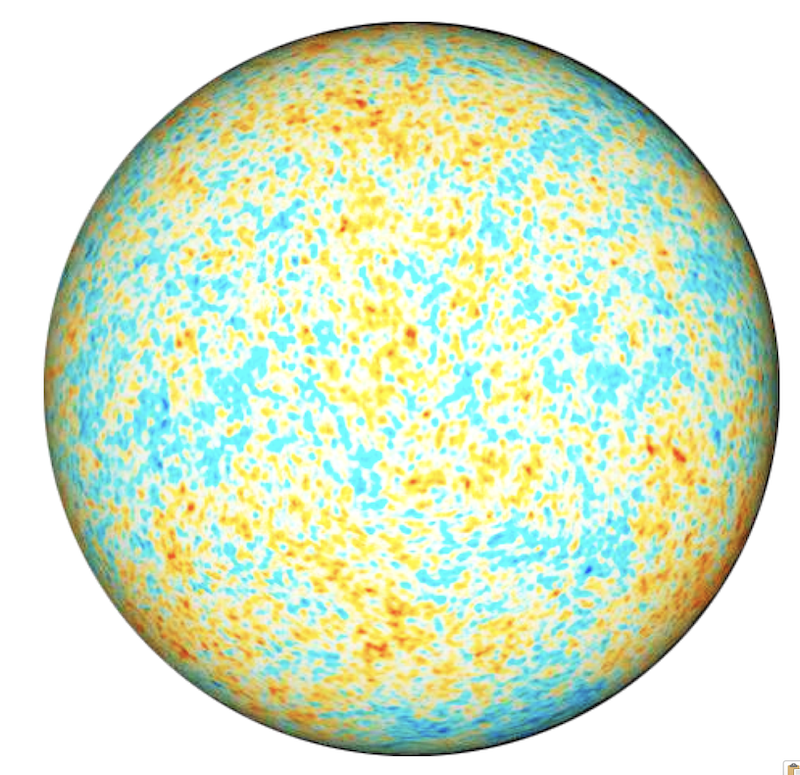
\includegraphics[width=0.9\linewidth]{figures/planck.png}
Planck 空间天文台观测到的宇宙微波背景辐射是 $\mathbb{S}^2$ 上的信号。
}
二维球面 $\Omega = \mathbb{S}^2$，其旋转群为{\em 特殊正交群} $\fG = \mathrm{SO}(3)$。
%
尽管选择该例是出于教学目的，但它实际上非常实用，并出现在大量应用中。例如，在天体物理学中，观测数据往往天然具有球面几何。此外，在化学应用中对分子建模并预测其性质时，球面对称性也十分重要，例如可用于虚拟药物筛选。
%\michael{ADD: molecules/astrophysics}


把球面上的点表示为三维单位向量 $\mathbf{u} : \|\mathbf{u}\|=1$ 后，群作用可以表示为 $3\times 3$ 正交矩阵 $\mathbf{R}$，并满足 $\mathrm{det}(\mathbf{R}) = 1$。因此，球面卷积可以写成信号与旋转后滤波器的内积：
$$
(x\star \theta)(\mathbf{R}) = \int_{\mathbb{S}^2} x(\textbf{u}) \theta(\mathbf{R}^{-1}\mathbf{u}) \mathrm{d}\mathbf{u}.
\marginnote{
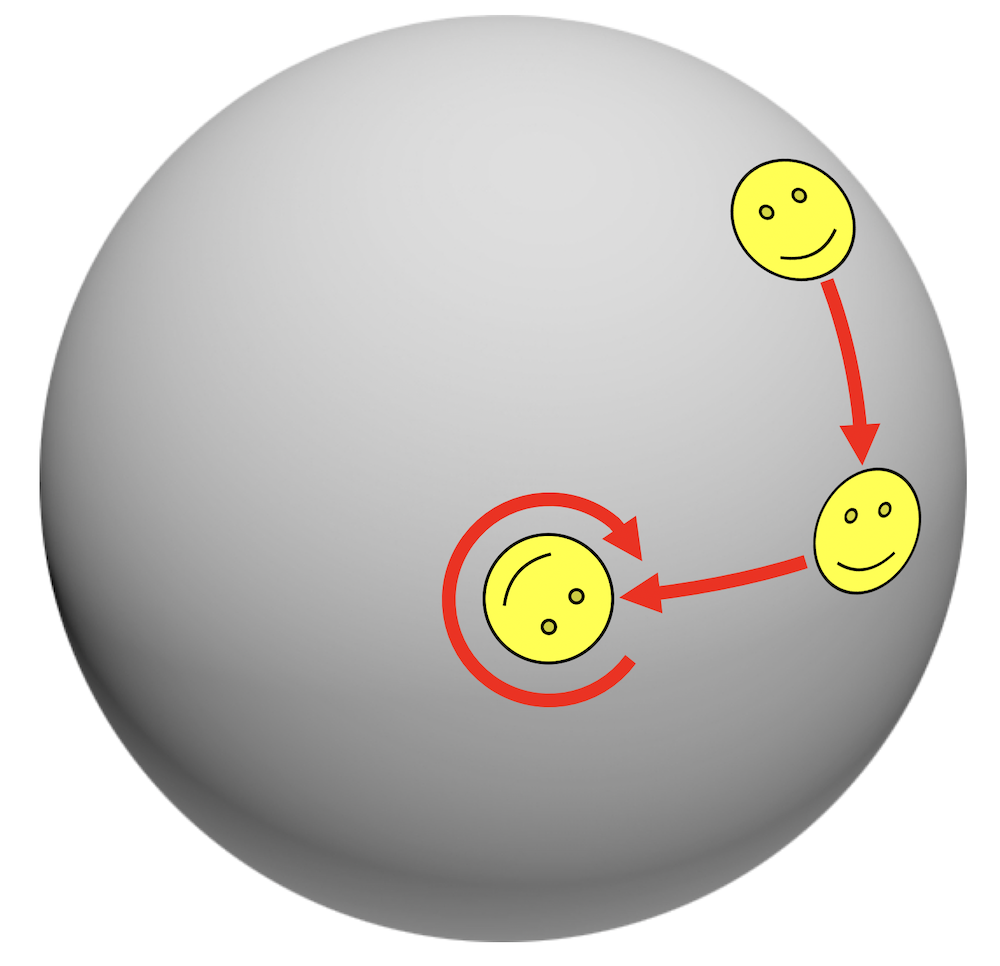
\includegraphics[width=0.9\linewidth]{figures/so3.png}
The action of $\mathrm{SO}(3)$ group on $\mathbb{S}^2$. Note that three types of rotation are possible; the $\mathrm{SO}(3)$ is a three-dimensional manifold.  
}
$$


首先应注意，此时群与域并不相同：群 $\mathrm{SO}(3)$ 是 Lie 群，事实上是三维流形；而 $\mathbb{S}^2$ 是二维流形。
%
因此，与前一个例子不同，这里的卷积是定义{\em 在} $\SO{3}$ {\em 而非} $\Omega$ {\em 上的}函数。

%\michael{\bf [ADD: a figure showing the difference between the sphere and SO(3) and why integration on S would give only isotropic filters.]}


这会带来重要的实际后果：在几何深度学习蓝图中，我们把后续算子应用于前一个算子的输出，以此串接多个等变映射（在深度学习术语中称为“层”）。
%
在平移情形下，可以依次应用多个卷积，因为它们的输出都定义在同一个域 $\Omega$ 上。
%
在一般设定下，由于 $x \star \theta$ 是定义在 $\fG$ 而非 $\Omega$ 上的函数，后续不能使用完全相同的运算——这意味着下一个运算必须处理{\em $\fG$ 上的信号}，即 $x \in \mathcal{X}(\fG)$。
%
群卷积的定义允许处理这种情形：
把域取为 $\Omega = \fG$，并让 $\fG$ 自身通过群作用 $(\fg, \fh) \mapsto \fg \fh$ 作用于它；该作用由 $\fG$ 的复合运算定义。
由此得到表示 $\rho(\fg)$，它作用于 $x \in \mathcal{X}(\fG)$，其作用方式为 $(\rho(\fg) x)(\fh) = x(\fg^{-1}\fh)$。\marginnote{$\fG$ 作用于定义在 $\fG$ 自身上的函数时，其表示称为 $\fG$ 的\emph{正则表示}。}
% where $\fg, \fh$ and their composition $\fg^{-1}\fh$ belong to the group $\fG$.
与之前一样，内积通过在域上积分%product of $x$ and $\psi$
信号与滤波器的逐点乘积来定义；
此时该域为 $\Omega = \fG$。
%
因此，在球面卷积的例子中，第二个卷积层具有如下形式：
$$
((x\star \theta)\star \phi)(\mathbf{R}) = \int_{\mathrm{SO}(3)} (x\star \theta)(\textbf{Q}) \phi(\mathbf{R}^{-1}\mathbf{Q}) \mathrm{d}\mathbf{Q}.
$$


%Now consider $\Omega = \R^2$ with  the group $\fG = \SE{2}$ of planar rotations and translations.\marginnote{$\SE{2}$ is called the {\em special Euclidean group} and is a subgroup of the Euclidean (isometry) group that additionally includes reflection. } 
%The first thing to note is that now the group elements (roto-translations) are not identical to the points on the domain. Consequently, in this case, unlike the previous example, the group convolution $x\star \psi$ given as the inner product between the signal and the transformed filter is a function {\em on} $\SE{2}$ {\em rather than on} $\Omega$. 

%\taco{TODO: Figure of SE2 group conv. Both planar to group, and group to group.}




%Our construction can be generalized to signals on any (locally compact) group $\fG$ and any $\Omega$ acted on by $\fG$ (in a sufficiently nice way).
%$\Omega$ is said to be a {\em homogeneous space} if for any two points $u, v \in \Omega$ one can be transformed into another, $u = \fg v$, by a symmetry $\fg \in \fG$. 
%that maps one to the other, .
%As noted before, for any such space $\Omega$, we have a regular representation $\rho(\fG)$ of $\fG$ acting on the space of signals $\mathcal{X}(\Omega)$. \michael{Bring the definition of homogeneous space earlier to Sec 1.2.1}
%
%As we will show in Chapter ???, for any two homogeneous spaces $\Omega$ and $\Omega'$ and a group $\fG$, one can define a convolution that maps between $\mathcal{X}(\Omega)$ and $\mathcal{X}(\Omega')$ in an equivariant manner, and indeed the most general linear equivariant map between these spaces is a convolution.

由于卷积涉及内积，而内积又需要在域 $\Omega$ 上积分，所以只能在规模较小（离散情形）或维数较低（连续情形）的域 $\Omega$ 上使用卷积。
% 
例如，可以在平面 $\R^2$（二维）、特殊正交群 $\SE{3}$（三维）或图的有限节点集合（$n$ 维）上使用卷积；但在实践中无法在置换群 $\Sigma_n$ 上执行卷积，因为该群含有 $n!$ 个元素。
%
同样，在更高维的群（如仿射群，其中包含平移、旋转、剪切和缩放，共有 $6$ 个维度）上积分，在实践中并不可行。
%
尽管如此，正如第~\ref{sec:gnn-intro} 节所见，通过处理定义在低维空间上的信号，仍可以为大群 $\fG$ 构造等变卷积；这里的低维空间为 $\Omega$，且 $\fG$ 作用于其上。
事实上，可以证明，两个域之间的任意等变线性映射 $f : \mathcal{X}(\Omega) \rightarrow \mathcal{X}(\Omega')$，其中两个域为 $\Omega, \Omega'$，都可以写成类似于这里所讨论群卷积的广义卷积。%\michael{Taco: I don't understand what you want to say here.}

其次，注意到上一节从卷积的移位等变性质推导出的 Fourier 变换，也可以通过把信号投影到对称群不可约表示的矩阵元素上，推广到更一般的情形。后续工作将对此展开讨论。
%
对于这里研究的 $\SO{3}$，这会产生{\em 球谐函数}与 {\em Wigner D-functions}，它们在量子力学和化学中有广泛应用。


最后指出支撑本节此前讨论的一项假设：无论 $\Omega$ 是网格、平面还是球面，我们都可以把任意一点变换为任意另一点；直观而言，这意味着域上的所有点“看起来都一样”。% by means of a rotation
%
具有这一性质的域 $\Omega$ 称为{\em 齐性空间}；对任意 $u, v\in \Omega$，都存在 $\mathfrak{g}\in\fG$ 使得
$
\mathfrak{g}.u = v\marginnote{The additional properties, $\mathfrak{e}.u = u$ and $\mathfrak{g} (\mathfrak{h}. u) = (\mathfrak{gh}). u$ are tacitly assumed here. }
$.
%
下一节将尝试放宽这一假设。

%Consider as given a space $\Omega$, such as $\Omega = \R^2$, $\Omega = \Z^2$, or $\Omega = S^2$ (the sphere).
%Furthermore, let $G$ be a group of symmetries acting on $\Omega$, such as the group of roto-translations acting on $\R^2$, or the group or 3D rotations acting on the sphere.
%The inputs and feature maps of our generalized CNN are modelled as signals on $\Omega$, defined as $\mathcal{X}_\Omega = \{f : \Omega \rightarrow \R\}$\marginnote{In practice one would usually want to use multiple channels $c$, i.e. $f : \Omega \rightarrow \R^c$ but to reduce clutter we consider a single channel / grayscale image for now.}.
%From the action of $G$ on $\Omega$, we can derive an action of $G$ on $\mathcal{X}_\Omega$:
%\begin{equation}
%	\rho(g) f(x) = f(g^{-1} x)
%\end{equation}
%When $G$ is the translation group, this is just the \emph{shift operator} defined in the previous section.
%Similarly, when $G$ is the roto-translation group, this operator tells us how to roto-translate an image of filter $f$.

%In order to match a filter and an image / feature map, we define an inner product:
%\begin{equation}
%    \langle f, \psi \rangle = \int_{\Omega} f(x) \psi(x) d\mu(x),
%\end{equation}
%where $\mu$ is an invariant measure on $\Omega$. % too technical?
%In the case where $\mu$ is discrete, the inner product is a sum over the ``dimensions'' $x$ of the product of the vector components $f(x) \psi(x)$. 

%Having defined how to transform filters and match patterns, we are ready to define the generalized convolution:
%\begin{equation}
%    \label{eq:group-conv}
%    f \star \psi(g) = \langle f, \rho(g) \psi \rangle = \int_\Omega f(x) \psi(g^{-1} x) %d\mu(x).
%\end{equation}

%Let's look at some examples.
%When $\Omega = \Z_n = \{1, \ldots, n\}$ and $G = \Z_n$ (i.e. we consider signals on $\Z_n$ and the group of cyclic shifts) as in the last section, we retrieve the usual discrete convolution.
%To see this, note that $g^{-1} x$ in the equation above means: invert the group element $g \in G$ (in this example, the inverse of $g \in \Z_n$ is $-g$) and then act on $x \in \Omega$ (in this example, we get $x - g$.
%So the equation boils down to $f \star \psi(g) = \sum_i f(i) f(i - g)$.

%Now consider $\Omega = \R^2$ and $G = \SE{2}$, the group of rotations and translations acting on the plane.
%The first thing to note is that $f \star \psi$ is a function on $G = \SE{2}$ rather than a function on $\Omega$.
%In the previous example $\Omega = G$ so the distinction does not matter, but here it does.
%The group convolution computes the similarity between the input and filter for each transformation of the filter.



%Since the feature map $f \star \psi$ is a function on $G$ rather than $\Omega$, we cannot use exactly the same operation for the second and higher layers of the network.
%The solution is easy enough, though: for the second layer we define $\Omega_2 = G$, so that the feature space consists of functions $f : G \rightarrow \R$.
%We again define a shift operator $\rho_2(g)$ acting on such functions by $(\rho(g) f)(h) = f(g^{-1} h)$, where now $g^{-1} h$ refers to composition in the group $G$ (c.f. $g^{-1} x$ for $x \in \Omega$ refering to the group action of $G$ on $\Omega$).
%With these definitions, the exact same Equation \ref{eq:group-conv} defines the group convolution for second and higher layers.

%As a final example, consider spherical CNNs.
%Here we take the domain $\Omega_1 = S^2$ (the sphere) for the input space, and $G = \SO{3}$ the rotation group as symmetries.

%\taco{TODO: all of the above should be more conversational. Maybe focus on one example?}

%\michael{Generalised Fourier transform using representation theory. Bring up again the notion of multidimensional frequencies and show here where it comes from. }


%\michael{{\bf Say something along the lines:} 
%The important difference between the above examples and the case of sets and graphs is that on the grid, plane, or sphere we can represent our group with a small number of parameters: in case case of $\Z_n$, this is just one index, in the case of $\mathbb{R}^2$, this is translation vector and rotation angle, and in the case of the sphere ... 
%
%Conversely, on sets or graphs, the permutation group does not have such a low-dimensional representation and has a combinatorial complexity. 

%Show again why on graphs we don't have multi-dimensional Fourier transform. 
%}

%\michael{Talk about homogeneous vs non-homogenous spaces, using the example of graphs. Make it a segway to the next section}


%[Fourier theory]


\subsection{测地线与流形}
\label{sec:geomanifoldsec}
%\michael{\bf [TACO: pls check if you are ok with this narrative. I start with homogeneous spaces, manifolds, then parallel transport. Then we can say that there is a broader view and talk about bundles in general]}

%\joan{
%Some high-level comments on what's written so far. 
%The generalization from groups to gauges is non-trivial, and I think it would be helpful to illustrate this extra level of generality with a running example. 
%In particular, an important innovation is that now we associate input data to certain vector fields on the domain; this is different from before. 
%It seems that this is the setting where the gauge equivariance is best motivated (unless I missed something), and I assume we can still use certain tasks from particle physics to motivate it.
%In other words, so far in our previous applications, the symmetry group acts on signals $\mathcal{X}(\Omega, \gV)$ only through $\Omega$, leaving the channels unchanged (just transporting them along the group action in $\Omega$). Now the situation is different and the gauge transformation is acting on the channels. 
%}

%\joan{I had a quick pass and the section reads very well; the build-up is coherent and objects are introduced keeping the intuition in mind (and adding figures to the margins will be even more helpful. 

%In particular, we can highlight that, contrary to the previous example of a fixed (curved) domain, many applications consider a variable geometric domain, and we wish to obtain signal representations that satisfy certain properties, namely (i) they are intrinsic, ie since the domain is defined only up to isometry, the signal representation should be invariant to isometries, and (ii) stability properties as this geometric domain changes. 
%These two aspects require introducing minimal elements of riemannian geometry 

%I have one comment/question though: currently we introduce the "minimal" elements of riemanian geometry that allow us to define convolutions and to describe the natural symmetries arising in manifold data (in particular isometry). 
%Would it be possible/convenient to highlight the invariance/stability priors early on, to motivate even further the need to introduce the different concepts (connection, parallel transport, isometries, geodesics, etc). In other words, the starting point is that we want to estimate a function $f$ defined over $\gX(\Omega, \R^s)$ that satisfies certain priors. The first and most natural prior is that $f$ is defined up to isometric transformations of $\Omega$. The second (if appropriate) is again the scale separation, ie local statistics in $x \in \gX(\Omega, \R^s)$ dominate. Then we explain how these priors lead again naturally to the GDL template by appropriately extending the notion of convolution. Additionally, it could be pertinent to describe how these priors relate to the stability of $f$ with respect to small changes in the metric structure of $\Omega$. 


%}


在上一个例子中，%domain $\Omega$ was the
球面 $\mathbb{S}^2$ \marginnote{旋转群 $\mathrm{SO}(3)$ 也是如此，因为它是{\em Lie 群}。}
是一个{\em 流形}，尽管它是一种特殊流形，
%: every point $u$ on $\mathbb{S}^2$ can be rotated into any other point $v$, intuitively meaning that all the points on the sphere ``look the same.'' % by means of a rotation  
%
%A domain $\Omega$ with such property is called a {\em homogeneous space}, where for any $u, v\in \Omega$ there exists %$\frak{g}\in\fG$ such that 
%$
%\frak{g}.u = v\marginnote{The additional properties, %$\frak{e}.u = u$ and $\frak{g}.(\frak{h}.u) = (\frak{gh}).u$ %are tacitly assumed here. }
%$.
%%
%Homogeneous spaces thus have a 
其齐性结构使它具有全局对称群。
%
遗憾的是，大多数流形并非如此，它们通常不具有全局对称性。
%
在这种情形下，无法直接定义 $\fG$ 在 $\Omega$ 上信号空间中的作用，也无法利用它使滤波器四处“滑动”，从而把卷积定义为经典构造的直接推广。
%. \joan{why would we want to translate signals in the manifold?}
%
尽管如此，流形确实具有两类不变性%symmetries
%various kinds of \emph{local} symmetries 
，本节将对此加以探讨：保持度量结构的变换，以及局部参考标架的变化。
%local \emph{gauge symmetries}, which we will now explore. 

尽管对许多机器学习读者而言，流形可能显得有些陌生，但它们在各种科学领域中其实非常常见。在物理学中，流形作为宇宙模型发挥核心作用——根据 Einstein 的广义相对论，引力源于时空的曲率，而时空被建模为伪 Riemann 流形。
%
在计算机图形学与视觉等较为“日常”的领域，流形是三维形状的常用数学模型。\marginnote{“3D”一词略有误导性，它指的是{\em 嵌入空间}。形状本身是二维流形（曲面）。}%
%
这类模型的应用范围十分广泛，从虚拟现实、增强现实以及通过“动作捕捉”获得的
特效，到研究蛋白质相互作用的结构生物学；蛋白质会像三维拼图块一样黏合在一起（化学术语称为“结合”）。
%
这些应用的共同之处，是使用流形表示某个三维对象的边界曲面。


这类模型之所以便利，有以下几个原因。\marginnote{
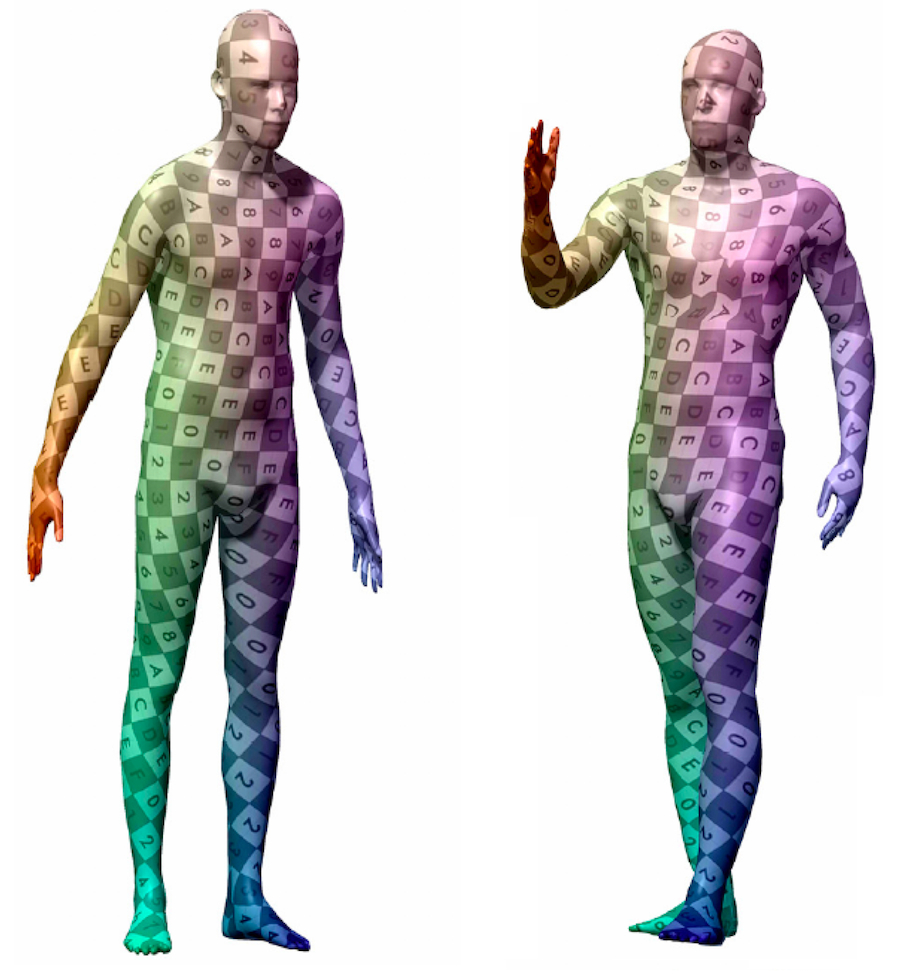
\includegraphics[width=0.9\linewidth]{figures/humans.png}
人体是以近似等距方式发生形变的非刚性对象实例。
}第一，它们可以紧凑地描述三维对象，无需像基于网格的表示那样为“空白空间”分配内存。
%
第二，它们允许忽略对象的内部结构。例如在结构生物学中，这一性质很有用，因为蛋白质分子的内部折叠通常与发生在分子表面的相互作用无关。
%
第三，也是最重要的一点，人们经常需要处理发生非刚性形变的{\em 可变形对象}。人体就是一例；计算机图形学与视觉中的许多应用，例如前述动作捕捉和虚拟化身，都要求{\em 形变不变性}。
这类形变可以很好地建模为保持（Riemann）流形内蕴结构的变换，即保持\emph{沿}流形测量的点间距离，而不考虑流形嵌入周围空间的方式。

%Here, we should emphasize that 
需要强调的是，%similarly to the case of graphs,
在几何深度学习蓝图中，流形属于{\em 可变域}设定，在这一意义上与图相似。我们将突出对域形变不变这一概念的重要性——这就是第~\ref{sec:geom_stab} 节所称的“几何稳定性”。
%
鉴于机器学习读者可能不太熟悉微分几何，我们将介绍讨论所需的基本概念；详细论述可参见 \cite{penrose2005road}。

%we have briefly mentioned before. 
%That is, unlike grid of homogeneous spaces we have discussed before where the domain can be assumed fixed and we are concerned with different signals on 

%\taco{Should we clarify why we need manifolds if we want deformation invariance? Also, should we call it deformation insensitivity? Since invariance would imply invariance to arbitrarily large deformations (just compose many small ones, each of which the net is invariant to.)}
%\michael{The proper term is isometry invariance. Isometry is understood in two senses: Riemannian (local metric=quadratic form on tangent space) and metric (geodesic distance). The two are equivalent on geodesically complete spaces due to Hopf-Rinow, which implies we can access the whole manifold through exp map from a single point. }

%\michael{STORY: we want to say that all models we build here are isometry-invariant, by virtue of being intrinsically constructed. This requires the definition of a Riemannian manifold. We can also refer to spectral techniques. 
%
%We then discuss gauges in this perspective, and then say that this is a much broader picture that does not need any metric, nor manifold, and can be defined on a bundle which is a topological construct. 
%}

%\joan{This is a good place to motivate geometric DL models that would fall beyond the homogeneous category: give a representative example that we can use throughout the rest of the section to guide the reader.} \michael{I think we focus this section on the domains, rather than on DL models. We should probably defer it to the discussion of Gauge CNNs.}


%\michael{Taco: why use $s$ and not $d$ for the manifold dimension? Do you want to decouple the feature dimension from the dimension of the manifold? } \joan{I switched from $d$ to $s$ since we used $d$ to refer to the dimensionality of the data and not the intrinsic dimension of the domain}
%
%\paragraph{Riemannian manifolds}
%\label{sec:manifolds}
%
%Since the formal definition of a manifold\marginnote{By `smooth' we mean differentiable suffient number of times, which is tacitly assumed for convenience. `Deformed' here means \emph{diffeomorphic}, i.e., we can map between the two neighbourhoods using a smooth and invertible map with smooth inverse. %, called a diffeomorphism. 
%%In this way, we can choose smooth coordinates for neighbourhoods of the manifold.
%} is somewhat involved, we 
%%defer its detailed discussion to Chapter ??? and 
%prefer to provide an intuitive picture at the expense of some precision. 
%%
%In this context, we can think of a (differentiable or smooth) manifold as a smooth multidimensional curved surface %(or higher dimensional space) 
%that is \emph{locally Euclidean} in the sense that any small neighbourhood around any point it can be deformed
%%\marginnote{`Deformed' here means \emph{homeomorphic to}, i.e. we can map between the neighbourhoods using a continuous and invertible map with continuous inverse. In fact, we will assume the manifold is smooth, in which case the map should be a diffeomorphism -- smooth and invertible with smooth inverse.}
%to a neighbourhood of $\R^s$; 
%%A crucial difference between a manifold\marginnote{We also tacitly assume the manifold to be smooth, i.e. having a $\mathcal{C}^\infty$-differentiable set of transition functions between local spaces.} and a Euclidean space is that a manifold is only {\em locally} Euclidean:  %
%%a small neighbourhood (open set) around each point $u \in \Omega$ is homeomorphic 
%%\marginnote{A {\em homeomorphism} is a continuous map with continuous inverse that preserves topological properties.}  to 
%%(topologically equivalent) to $\mathbb{R}^s$; 
%%
%%by a homeomorphism called a {\em chart}; 
%%the dimension $d$ is that of the manifold, which 
%in this case the manifold is said to be $s$-{\em dimensional}. 
%%
%%The composition of two charts (or more precisely, a chart and an inverse of a chart) allows to transition between the local 
%%
%%
%%Since the manifold is smooth, 
%This allows us to 
%locally approximate the manifold around point $u$ through the \emph{tangent space} $T_u\Omega$.  %and called the {\em tangent space}.
%The latter can be visualized by thinking of a prototypical two-dimensional manifold, the sphere, and attaching a plane to it at a point: with sufficient zoom, the spherical surface will seem planar. 
%% This analogy however should not be taken literally, as manifolds are abstract objects existing on their own without any geometric realization.  % Taco: this may be a bit confusing for newbies
%%
%\marginnote{Formally, the tangent bundle is the {\em disjoint union} $\displaystyle T\Omega = \bigsqcup_{u\in \Omega} T_u\Omega$.} The collection of all tangent spaces is called the {\em tangent bundle}, denoted $T\Omega$; we will dwell on the concept of bundles in more detail in Section~\ref{sec:gauges}. 
%%later and also in Chapter ???.
%
%
%
%A {\em tangent vector}, which we denote by $X\in T_u\Omega$, can be thought of as a local displacement from point $u$. 
%%In order to give it a sense of {\em direction}, 
%In order to measure the \emph{lengths} of tangent vectors and  \emph{angles} between them, %, and {\em volumes}, 
%%
%\marginnote{A bilinear function $g$ is said to be {\em positive-definite} if $g(X,X)>0$ for any non-zero vector $X\neq 0$. If $g$ is expressed as a matrix $\mathbf{G}$, it means $\mathbf{G} \succ 0$. The determinant $|\mathbf{G}|^{1/2}$ provides a local volume element, which does not depend on the choice of the basis. } 
%%
%we need to equip the tangent space with additional structure, expressed as a 
%positive-definite bilinear function
%$g_u: T_u\Omega \times T_u\Omega \rightarrow \mathbb{R}$ depending smoothly on $u$. Such a function is 
%called a {\em Riemannian metric}, in honour of Bernhardt Riemann who introduced the concept in 1856, and can be thought of as an inner product on the tangent space, $\langle X, Y \rangle_u = g_u(X,Y)$, which is an expression of the angle between any two tangent vectors $X, Y \in T_u\Omega$. 
%%
%The metric also induces a norm $\| X \|_u = g_u^{1/2}(X,X)$ allowing to locally measure lengths of vectors. 
%
%
%
%We must stress that tangent vectors 
%\marginnote{Unfortunately, too often vectors are identified with their coordinates. 
%%, which in our view constitutes a crime against humanity. 
%To emphasize this important difference, we use $X$ to denote a tangent vector and $\mathbf{x}$ to denote its coordinates. }
%are abstract geometric entities that exists in its own right and are {\em coordinate-free}. If we are to express a tangent vector $X$ numerically as an array of numbers, we can only represent it as a list of coordinates $\mathbf{x}=(x_1, \hdots, x_s)$ {\em relative to some local basis} $\{ X_1, \hdots X_s \} \subseteq T_u\Omega$.   
%%
%Similarly, the metric can be expressed as an $s\times s$ matrix $\mathbf{G}$ with elements $g_{ij} = g_u(X_i,X_j)$ w.r.t that basis. %; however, we stress that the definition of Riemannian metric does not rely on any particular choice of basis %all our definitions are coordinate-free and exist independently of any basis choice
%%(this will be the centrepiece of the following section). 
%
%%that allows to measure length, angle, and volume in the tangent space. 
%%
%
%
%
%%an {\em inner product}.
%%In differential geometry, an inner product on $T_u\Omega$ depending smoothly on $u$ is called a {\em Riemannian metric}, in honour of Bernhardt Riemann who introduced the concept in 1856. %
%%We will denote a Riemannian metric as a$g_u: T_u\Omega \times T_u\Omega \rightarrow \mathbb{R}$ that allows to measure length, angle, and volume in the tangent space. 
%%
%
%%
%%of a vector $$
%%
%%angle between two tangent vectors $x,y \in T_u\Omega$, (expressed %as $\cos^{-1}\left( \frac{\g_u(x,y)$) and a length of the 
%
%
%A manifold equipped with a metric is called a
%{\em Riemannian manifold} and properties that can be expressed entirely in terms of the metric are said to be {\em intrinsic}. %
%This is a crucial notion for our discussion, as according to our template, we will be seeking to construct functions acting on signals defined on $\Omega$ that are invariant to metric-preserving transformations called {\em isometries} that, roughly speaking, deform the manifold without affecting its local structure. If such functions can be expressed in terms of intrinsic quantities, they are automatically guaranteed to be isometry-invariant and thus unaffected by isometric deformations. 
%%
%These results can be further extended to dealing with approximate isometries; this is thus an instance of the geometric stability (domain deformation) discussed in our blueprint. 
%
%
%%\taco{Taco: here we should probably make clear that we are not talking about symmetries in the sense of automorphisms, i.e. maps $\Omega \rightarrow \Omega$ that preserve the metric, but about isomorphisms, i.e. maps $\Omega \rightarrow \Omega'$ that preserve the metric. Note that we do not yet discuss this in the template, but as discussed we should.} 
%
%%\michael{Approx isometry - geometric stability}
%
%While, as we noted, the definition of a Riemannian manifold does not require a
%geometric realization in any space, it turns out that any smooth Riemannian manifold can be realized as a subset of a Euclidean space of sufficiently high dimension (in which case it is said to be `embedded' in that space) by using the structure of the Euclidean space to induce a Riemannian
%metric.\marginnote{This result is known as the {\em Embedding Theorem}, due to John Forbes Nash, who became a household name after the Hollywood movie The Beautiful Mind. The paper folding art of origami is a manifestation of different isometric embeddings of the planar surface in $\mathbb{R}^3$. \vspace{4mm}
%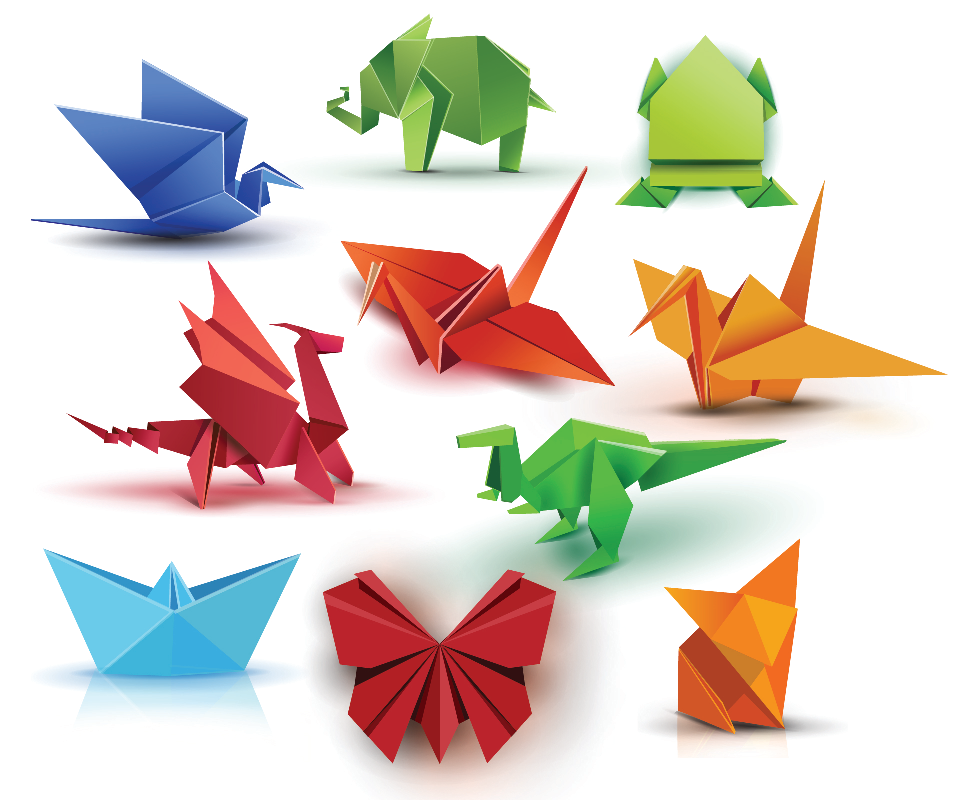
\includegraphics[width=1\linewidth]{figures/origami.pdf}
%}  Such an embedding is however not necessarily unique -- as we will see in the following, two different isometric 
%realizations of a Riemannian metric are possible. 
%%called {\em isometries}.
%
%
%
%
%
%\paragraph{Covariant derivative and Parallel transport}
%%
%Since we are interested in signals defined on $\Omega$, we need to provide the proper notion of scalar-
%%\marginnote{We will use the same notation for tangent and vector fields, the distinction between which will be clear from the context.} 
%and vector-valued functions on manifolds. 
%%
%A {\em scalar field} is a function of the form $x: \Omega\rightarrow \mathbb{R}$. 
%%
%%scalar-valued function  (often called a {\em scalar field}) $x: \Omega\rightarrow \mathbb{R}$ on the manifold. The space of 
%Scalar fields form a vector space $\mathcal{X}(\Omega, \mathbb{R})$ that can be equipped with the inner product %of scalar fields
%\begin{equation}
%\langle x, y \rangle = \int_\Omega x(u) y(u) \mathrm{d}u,
%\label{eq:inner_scalar}   
%\end{equation}
%%
%where $\mathrm{d}u$ % = \sqrt{\det g}$
%%\marginnote{More rigorously speaking, the volume form requires an inner product (i.e. Riemannian metric) and {\em orientation} (`handedness'). } 
%is the volume element induced by the Riemannian metric. 
%%
%%
%A (tangent) {\em vector field} is a function of the form $X: \Omega \rightarrow T\Omega$  assigning to each point a tangent vector in the respective tangent space, $u\mapsto X(u)\in T_u\Omega$.  
%%
%Vector fields also form a vector space $\mathcal{X}(\Omega, T\Omega)$ with the inner product defined through the Riemannian metric, 
%%
%\begin{equation}
%\langle X, Y \rangle = \int_\Omega g_u(X(u), Y(u)) \mathrm{d}u. \label{eq:inner_vector}   
%\end{equation}
%
%
%Another way to think of (and actually {\em define}) vector fields is as a generalised notion of derivative. 
%%
%In classical calculus, one can locally linearise a (smooth) function through the {\em differential} $\mathrm{d}x(u) = x(u+\mathrm{d}u) - x(u)$, which provides the change of the value of the function $x$ at point $u$ as a result of an inifinitesimal displacement $\mathrm{d}u$. 
%%
%However, in our case using this  definition na{\"i}vely brings up two problems: First, expressions of the form ``$u+\mathrm{d}u$'' are meaningless on manifolds, since there is no global vector space structure. 
%%, preventing us from adding or subtracting two points on $\Omega$. 
%%
%%
%A second problem arises when trying to take derivatives of vector fields, as one would need to subtract vectors belonging to tangent spaces at {\em different points}, while subtraction is only define \emph{within} a single vector space. 
%
%
%
%
%
%The solution to the first problem is to use tangent vectors as a model of local infinitesimal displacement. 
%%in order to provide a proper generalization of the differential on manifolds. 
%%
%Given a smooth scalar field $x\in \mathcal{X}(\Omega,\mathbb{R})$, we can think of a (smooth) vector field as a linear map $Y:\mathcal{X}(\Omega,\mathbb{R}) \rightarrow \mathcal{X}(\Omega,\mathbb{R})$ satisfying the properties of a {\em derivation}: 
%$Y(c) = 0$ for any constant $c$ (corresponding to the intuition that constant functions have vanishing derivatives), $Y(x+z) = Y(x) + Y(z)$ (linearity), and $Y(xz) = Y(x)z + xY(z)$ ({\em product} or {\em Leibniz rule}), for any smooth scalar fields $x,z \in \mathcal{X}(\Omega,\mathbb{R})$. 
%%
%It can be shown that one can use these properties to define vector fields axiomatically. 
%%
%The differential of $x$ can be defined as an operator $\mathrm{d}x : T\Omega \rightarrow \mathbb{R}$ of the form
%$$
%\mathrm{d}x(Y) = Y(x),
%$$
%which can be interpreted as follows: the change of $x$ as the result of displacement $Y \in T_u\Omega$ at point $u$ is given by $\mathrm{d}x(Y)$. 
%%
%It is thus an extension of the classical notion of {\em directional derivative}. 
%%
%Importantly, this construction {\em does not use the Riemannian metric whatsoever} and can thus be generalised to a broader construction of bundles discussed in the next section. 
%
%
%
%At each point $u$, the differential operator $\mathrm{d}x_u$ can be regarded as a {\em linear functional} acting on tangent vectors $X \in T_u\Omega$. Linear functionals on a vector space are called {\em dual vectors} or {\em covectors}; if in addition we are given an inner product (Riemannian metric), a dual vector can always be represented as 
%\marginnote{This is a consequence of the Riesz-Fr{\'e}chet Representation Theorem, by which every dual vector can be expressed as an inner product with a vector. } 
%$$
%\mathrm{d}x_u (X)  = g_u(\nabla x(u), X).
%$$ 
%The representation of the differential at point $u$ is a tangent vector $\nabla x(u) \in T_u \Omega$ called the (intrinsic) {\em gradient} of $x$; similarly to the gradient in classical calculus, it can be thought of as the direction of the steepest increase of $x$. 
%%
%%More generally, the gradient can be thought of as an operator $\nabla : $
%
%
%
%
%In a similar way, we can axiomatically define the {\em covariant derivative} $\nabla_Y X$ of a smooth vector field $X$ along another smooth vector field $Y$ as an operator  
%$\nabla : T\Omega \times T\Omega \rightarrow T\Omega$ %associating the vector fields $(X,Y) \mapsto \nabla_Y X$ and satisfying the following properties: 
%of the following form:
%
%
%\begin{tcolorbox}[width=\linewidth,
%              boxsep=0pt,
%              left=7.5pt,
%              right=7.5pt,
%              top=7.5pt,
%              bottom=7.5pt,
%              arc=0pt,
%              boxrule=0pt,toprule=0pt,
%              colback=boxgray,
%              ]%%
%A  {\em covariant derivative} (or {\em connection}) is a map $(X,Y) \mapsto \nabla_Y X$
%satisfying, 
%for all smooth scalar fields $x, y \in \mathcal{X}(\Omega, \mathbb{R})$ and smooth vector fields $X, Y, Z \in \mathcal{X}(\Omega, T\Omega)$, 
%the following axioms: \vspace{3mm}\\
%%\begin{enumerate}
%%\item 
%\noindent {\em Linearity (w.r.t. first argument):} 
%$\nabla_{xY + yZ}(X) = \nabla_Y(X)x + \nabla_Z(X)y$.\vspace{2mm}\\
%\noindent  {\em Additivity (w.r.t. second argument):}
%%\marginnote{For an {\em affine connection}, the additivity requirement is dropped. } 
%$\nabla_Y(X+Z) = \nabla_Y X + \nabla_Y Z$.\vspace{2mm}\\
%\noindent  {\em Product rule:} $\nabla_Y(zX) = z \nabla_Y(X) + \mathrm{d}z(Y) X$, where for scalar fields the covariant derivative coincides with the differential,  
%%, where in the second term  
%$\nabla_Y(z) = \mathrm{d}z(Y)$.%\vspace{2mm}
%%
%%    \noindent  
%%\end{enumerate}
%
%\end{tcolorbox}
%
%Covariant derivative allows {\em parallel transport}, or a way of moving tangent vectors along a curve so they are ``pointing in the same direction''.  
%%
%Given a smooth curve $\gamma : [0,T] \rightarrow \Omega$, a vector $X$ is said to be parallel transported along $\gamma$ if $\nabla_{\gamma'(t)} X(\gamma(t)) = 0$ for $t \in [0,T]$, where $\gamma'(t) \in T_{\gamma(t)} \Omega$ is the tangent to the curve. 
%%
%Intuitively, this implies that the vector remains `constant'\marginnote{
%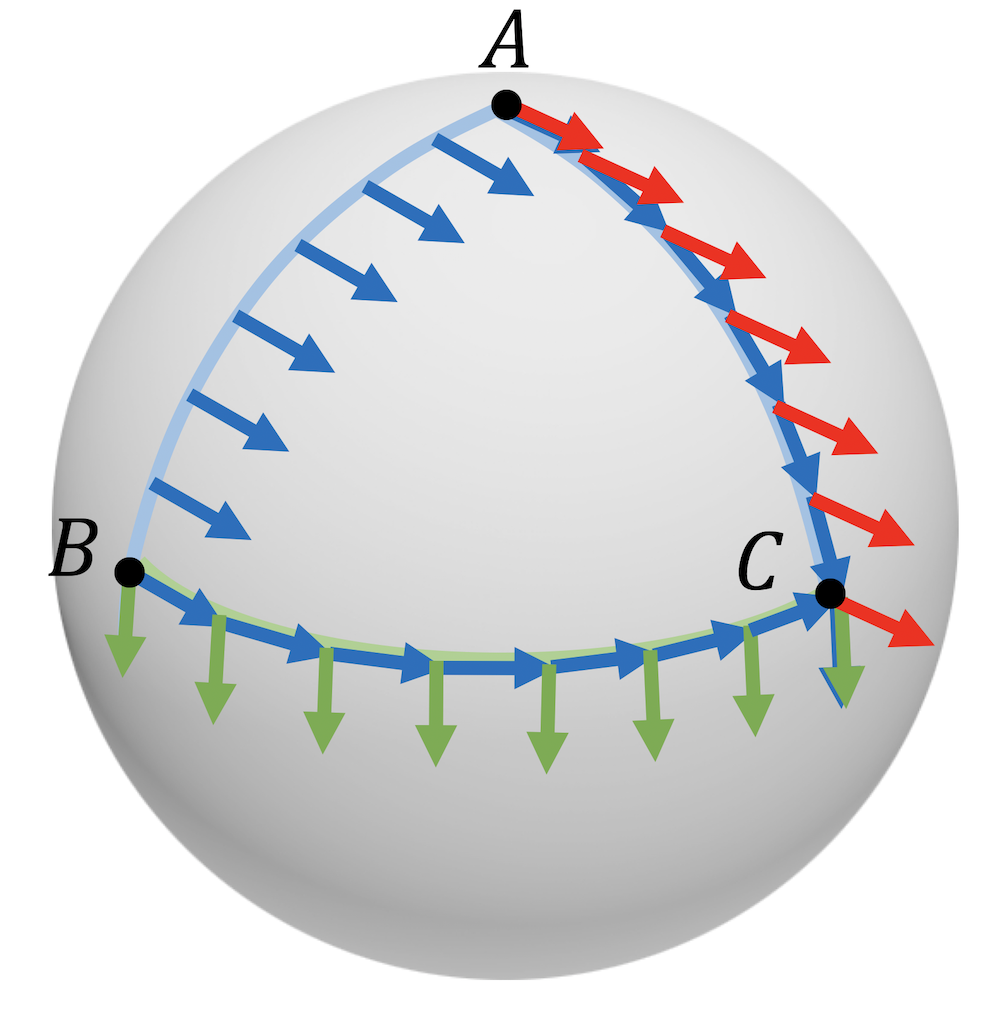
\includegraphics[width=0.9\linewidth]{figures/parallel.png}
%Euclidean transport of a vector from A to C makes no sense on the sphere, as the resulting vectors (red) are not in the tangent plane. Parallel transport from A to C (blue) rotates the vector along the path. It is path dependent: going along the path BC and ABC produces different results.  
%} (the derivative vanishes) for a small displacement along the curve. 
%%
%The result of the transport is path-dependent, which is best visualised on the sphere (see insert): moving a vector from the north pole to the equator along two different curves produces different results.
%%
%The name `connection' stems from the fact that parallel transport defines a linear isomorphism between tangent spaces along the curve $\gamma$, that is, a way to transport vectors from $T_{\gamma(0)}\Omega$ to $T_{\gamma(T)}\Omega$, thereby `connecting' these spaces.
%
%
%%which transports its tangent along itself 
%
%
%%perform  
%%of tangent vectors by (in this way, it ``connects'' two tangent spaces at different points, hence the alternative name `connection').  
%
%It is important to note that the definition of the covariant derivative  %and geodesic 
%does not rely on the metric, and  
%in fact, is an abstract construction that extends beyond Riemannian manifolds. %there are multiple ways to define one.  
%%
%When one is given a Riemannian metric, of particular interest is a special kind of covariant derivative called the {\em Levi-Civita connection}, after the Italian mathematician Tullio Levi-Civita who introduced the notion in 1917. %\marginnote{}
%%
%
%
%\begin{tcolorbox}[width=\linewidth,
%              boxsep=0pt,
%              left=7.5pt,
%              right=7.5pt,
%              top=7.5pt,
%              bottom=7.5pt,
%              arc=0pt,
%              boxrule=0pt,toprule=0pt,
%              colback=boxgray,
%              ]%%
%The {\em Levi-Civita connection} on a Riemannian manifold with metric $g$ is a connection $\nabla$ that additionally satisfies the following properties:
%\vspace{3mm}\\
%%\begin{enumerate}
%%\item 
%    \noindent  {\em Torsion free:} \marginnote{Roughly, {\em torsion} describes how tangent vectors twist about the curve when parallel transported, and {\em curvature} how they roll along it. }
%$\nabla_X Y - \nabla_Y X = [X,Y]$, where the tangent vector field $[X,Y] \in \mathcal{X}(\Omega, T\Omega)$ is the 
%{\em commutator} (also known as the {\em Lie bracket} or {\em Lie derivative}), defined by its action on scalar fields 
%$$[X,Y](z) = X(Y(z)) - Y(X(z)).$$
%%\vspace{2mm}\\
%%    
%\noindent {\em Preserves the metric:}\marginnote{Connection with this property is also known as {\em metric} or {\em metric-compatible}.} 
%$\nabla g = 0$, which is understood as 
%$$
%(\nabla_X g)(Y,Z) = X(g(Y,Z)) - g(\nabla_X Y, Z) - g(Y, \nabla_X Z) = 0.
%$$
%for any smooth $X, Y$, and $Z$. 
%
%\end{tcolorbox}
%
%
%%
%%
%The condition $\nabla g = 0$ (metric compability) implies that the metric remains invariant under parallel transport, i.e., parallel transport preserves the length of the tangent vectors (and is thus an isometry). 
%%
%The torsion-free properties make the Levi-Civita connection {\em unique}, a result known as the Fundamental Theorem of Riemannian Geometry. 
%%
%%\marginnote{
%For this reason, in Riemannian geometry the term `connection' is usually synonymous with the Levi-Civita connection, which can be considered a `canonical' connection.
%
%%guaranteeing that every Riemannian manifold admits a unique Levi-Civita connection, making it thus the `canonical' one. 
%
%
%
%
%%\taco{I think the notion of Torsion will be difficult to understand for newbies. Also, we are differentiating a tensor field g which I think we have not explained yet.
%
%%We could consider just mentioning the LC connection and explaining that parallel transport defined wrt it will not change the length of tangent vectors. We can also say that if another condition (Torsion free) is satisfied, there is a unique LC connection, without formalizing it.}
%
%
%
%\paragraph{Geodesics and Exponential map}
%
%A curve $\gamma$ along which parallel transport preserves the tangent vector to the curve,\marginnote{From the Greek \textgreek{geodai\textsigma{}{\'i}a}, literally `division of Earth'.}  i.e., $\nabla_{\gamma'} \gamma' = 0$ is called {\em geodesic}.
%%
%Locally at a point $u$, it is always possible to define a unique geodesic in a given direction $X$, i.e. a smooth curve $\gamma_X : [0,T] \rightarrow \Omega$ satisfying $\gamma(0) = u$ and $\gamma'(0) = X$, for some small $T>0$. 
%%
%%
%This\marginnote{Here, $B_r(0)$ is a ball of radius $r$ around the origin. Note that geodesic completeness does not necessarily guarantee that $\exp$ is a diffeomorphism -- the largest radius $r$ about $u$ for which $\exp_u(B_r(0) \subseteq T_u\Omega)$ is mapped diffeomorphically is called the {\em injectivity radius}. } gives a natural mapping from (a subset of) the tangent space $T_u \Omega$ to $\Omega$ called the {\em exponential map} $\exp : B_r(0) \subset T_u\Omega \rightarrow \Omega$, which is defined by taking a unit step along the geodesic in the direction $X$, i.e., $\exp_u(X) = \gamma_X(1)$. %
%%
%%
%When $\gamma_X(t)$ is defined for all $t\geq 0$ (that is, we can shoot the geodesic from a point $u$ for as long as we like), the manifold is said to be {\em geodesically complete} and the exponential map is defined on the whole tangent space.
%%
%Since compact manifolds are geodesically complete, we can tacitly assume this convenient property. 
%
%
%
%%
%On Riemannian\marginnote{It is tacitly assumed that curves are given in {\em arclength parametrisation}, such that $\| \gamma' \| = 1$ (constant velocity).} manifolds with the Levi-Civita connection, one can show geodesics to be {\em length-minimising curve}, 
%%
%i.e., a geodesic $\gamma$ minimises the length functional 
%%
%$$
%L(\gamma) = \int_{0}^T \| \gamma'(t) \| \mathrm{d}t =  \int_{0}^T g_u^{1/2} (\gamma'(t), \gamma'(t)) \mathrm{d}t 
%$$
%%
%among all curves with endpoints $u = \gamma(0)$ and $v=\gamma(T)$. 
%%
%%
%Readers familiar with metric geometry are probably more used to this definition of geodesics as shortests paths. 
%%
%In fact, \marginnote{Hopf-Rinow Theorem thus estabilishes the equivalence between geodesic and metric completeness, the latter meaning every Cauchy sequence converges.} a result known as the Hopf-Rinow Theorem guarantees that geodesically complete manifolds are also {\em complete metric spaces}, in which one can realise a metric (called the {\em geodesic distance})  between any pair of points $u,v$ as the length of the shortest path between them
%$$
%d_g(u,v) = \min_{\gamma} L(\gamma) \quad\quad \text{s.t.} \quad\quad \gamma(0) = u, \,\, \gamma(T) = v,
%$$
%which exists (i.e., the minimum is attained).\marginnote{To avoid confusion with the Riemannian metric, we will use the term `distance'. Our notation $d_g$ makes the distance depend on the Riemannian metric, though the definition of $L$. }
%%
%Importantly, geodesic distances are intrinsic, being dependent solely on the Riemannian metric. 
%
%
%%The term `geodesic' is also used in metric geometry, where it is defined as the shortest path. In the setting described here the two meanings coincide. }
%
%
%%i.e., the two notions of `geodesic' used somewhat differently in differential and metric geometry
%
%
%
%
%
%%===
%%
%%
%%For a smooth scalar field\marginnote{Linear functionals acting on vectors are called {\em dual vectors} or {\em covectors}. By the Riesz-Fr{\'e}chet Representation Theorem, every covector can be expressed as an inner product with a vector. } $x: \Omega \rightarrow \mathbb{R}$, the differential can be thought of as an operator $dx : T\Omega \rightarrow \mathbb{R}$ acting on tangent fields. At each point, the differential can be expressed as a linear functional acting on tangent vectors
%%$dx(u)  = g_u(\nabla x(u), \cdot)$. 
%%%
%%%
%%Given a smooth vector field $Y$, 
%%the {\em covariant derivative} $\nabla_Y x$ of $x$ {\em along} $Y$ is defined as 
%%$(\nabla_Y x)(u) = g_u(\nabla x(u), Y(u))$
%%and is a generalisation of the corresponding notion in classical calculus. 
%%%
%%%The change of the value of $x$ as the result of 
%%%displacement $y \in T_u\Omega$ at point $u$ is thus given by applying the form to the tangent
%%%vector, $dx(u) y = g_u(\nabla x(u), y)$, and can be thought
%%%of as an extension of the notion of the classical directional
%%%derivative.
%%%
%%The vector field $\nabla x$ is called the (intrinsic) {\em gradient} of $x$; at each point, it indicates the direction of the steepest increase of $x$. 
%%%
%%%The symbol $\nabla$ can be though of as an operator acting on scalar fields and producing vector fields defined above.  
%%
%%
%%Given two smooth vector fields $x$ and $y$, the covariant derivative $\nabla_y x$ of $x$ along $y$
%%
%%
%%
%%
%%Connection is defined as an abstract map $\nabla : T\Omega \times T\Omega \rightarrow T\Omega$ associating $(x,y) \mapsto \nabla_y x$ in a way that is linear w.r.t. both $x$ and $y$ and also satisfies the {\em product rule} $\nabla_y(xz) = x\nabla_y z + z \nabla_y x$ for any vector fields $x,y$ and scalar field $z$. 
%%
%%
%%
%%When the manifold is embedded in a Euclidean space, the covariant derivative coincides with the standard Euclidean directional derivarive projected onto the tangent space. 
%%
%%
%%
%%
%%
%%
%%%known as the {\em pushforward} $d\eta : T\Omega \rightarrow T\Omega'$.  
%%
%%
%%
%%the notion of derivative describes how the value of a function changes with an infinitesimal change of its
%%argument. 
%%
%%
%%One of the big differences distinguishing classical
%%calculus from differential geometry is a lack of vector space
%%
%%
%%structure on the manifold, prohibiting us from na\"{i}vely using
%%expressions like $f(x+dx)$. The conceptual leap that is required
%%to generalize such notions to manifolds is the need to work
%%locally in the tangent space
%%
%%
%%
%%
%%
%%
%%
%%
%%
%%
%
%
%
%
%
%\paragraph{Isometries}
%Consider now a deformation of our manifold $\Omega$ into another manifold $\Omega'$ with a Riemannian metric $h$.
%%
%We will assume this map to be a diffeomorphism $\eta: (\Omega, g) \rightarrow (\Omega', h)$ between manifolds.   
%%
%Its differential $\mathrm{d}\eta : T\Omega \rightarrow T\Omega'$ defines a map between the respective tangent bundles (referred to as {\em pushforward}), such that   
%%\marginnote{The pushforward is what is called a {\em bundle map}.}
%at a point $u$, we have $\mathrm{d}\eta_u : T_u \Omega \rightarrow T_{\eta(u)}\Omega'$, %which allows to interpret it as follows: 
%%
%interpreted as before: 
%if we make a small displacement from point $u$ by tangent vector $X \in T_u \Omega$, the map $\eta$ will be displaced from point $\eta(u)$ by tangent vector $\mathrm{d}\eta_u(X) \in T_{\eta(u)}\Omega'$. 
%
%
%Since the pushforward provides a mechanism to associate tangent vectors on the two manifolds, it allows to {\em pullback }\marginnote{Pushforward and pullback are adjoint operators $\langle \eta^* \alpha, X \rangle = \langle \alpha, \eta_*X \rangle$ where $\alpha \in T^*\Omega$ is a {\em dual vector field}, defined at each point as a linear functional acting on $T_u\Omega$ and the inner products are defined respectively on vector and dual vector fields. } the metric $h$ from $\Omega'$ to $\Omega$, 
%$$
%(\eta^*h)_u(X,Y) = h_{\eta(u)}(\mathrm{d}\eta_u(X), \mathrm{d}\eta_u(Y))
%$$ 
%%
%If the pullback metric coincides at every point with that of $\Omega$, i.e., $g = \eta^*h$, the map $\eta$ is called  (a Riemannian) {\em isometry}. % (metric-preserving). 
%%
%For two-dimensional manifolds (surfaces), isometries can be intuitively understood as inelastic deformations that deform the manifold without `stretching' or `tearing' it. 
%
%
%
%By virtue of their definition, isometries preserve intrinsic structures such as geodesic distances, which are expressed entirely in terms of the Riemannian metric. % and Gaussian curvature.
%%
%Therefore, we can also understand isometries from the position of metric geometry,\marginnote{The Myers–Steenrod Theorem establishes that the converse is also true on connected manifolds: every metric isometry is also a Riemannian isometry. } 
%as distance-preserving maps {\em between metric spaces} $\eta : (\Omega, d_g) \rightarrow (\Omega', d_h)$, in the sense that 
%$$
%d_g (u,v) = d_h(\eta(u),\eta(v)) 
%$$
%for all $u,v \in \Omega$, 
%or more compactly, $d_g = d_h \circ (\eta \times \eta)$. 
%%where $d_g, d_g$ are the geodesic distances induced by the respective Riemannian metrics $g, h$. 
%%
%
%%[Gauss Theorema Egregium, definition of curvature through perimeter defect, pizza example]
%
%
%A particular case of the above is a diffeomorphism  of the domain itself, which we will denote by $\tau \in \mathrm{Diff}(\Omega)$. We will call it a Riemannian  \mbox{(self-)isometry} if the pullback metric satisfies $\tau^* g = g$, or a metric (self-)isometry if $d_g = d_g\circ (\tau \times \tau)$.
%%
%Not surprisingly, isometries form a group with the composition operator denoted by $\mathrm{Iso}(\Omega)$ and called the {\em isometry group}; the identity element is the map $\tau(u) = u$ and the inverse always exists (by definition of $\tau$ as a diffeomorphism). 
%%
%Self-isometries are thus {\em intrinsic symmetries} of manifolds.
%
%
%%Continuous symmetries on manifolds are infinitesimally generated
%%%\marginnote{More correctly, Killing fields are the infinitesimal generators of continuous symmetries. } 
%%by special tangent vector fields called {\em Killing fields}, named after Wilhelm Killing. A field $X$ is Killing if the  Lie derivative\marginnote{The Lie derivative in this case is a derivative of forms. For scalar and vector fields, it coincides with the covariant derivative $\mathcal{L}_X y = \nabla_X y$ and the commutator $\mathcal{L}_X Y = [X,Y]$, respectively. } of the Riemannian metric along it vanishes, $\mathcal{L}_X g = 0$, which is interpreted as 
%%%
%%$$
%%\mathcal{L}_X g(Y,Z) = g(\nabla_Y X, Z) + g(Y,\nabla_Z X) = 0
%%$$
%%for any smooth tangent fields $Y, Z$. 
%%%
%%We can recap that like we mentioned in Section~\ref{sec:symmetries}, we can regard symmetries as automorphisms (self-maps) preserving additional structure: either the local Riemannian metric, or global geodesic distances between pairs of points. 
%%%\taco{Do we need Killing fields? It's interesting but I worry that we'd need to properly introduce Lie derivatives to make it understandable.} \michael{Lets keep them for now}
%%%OK :)
%



\paragraph{Riemann 流形}
\label{sec:manifolds}

由于流形的形式定义\marginnote{“光滑”是指可微足够多次；为方便起见，我们默认采用这一假设。这里的“形变”是指\emph{微分同胚}，即两个邻域之间存在光滑可逆映射，且其逆映射也光滑。%, called a diffeomorphism.
%In this way, we can choose smooth coordinates for neighbourhoods of the manifold.
}较为复杂，我们
%defer its detailed discussion to Chapter ??? and 
宁愿牺牲一些精确性，给出直观图景。
%
在这里，可以把（可微或光滑）流形看作一个光滑的多维弯曲曲面%(or higher dimensional space)
，它\emph{局部 Euclidean}；也就是说，任意一点附近的任意小邻域都可以形变为
%\marginnote{`Deformed' here means \emph{homeomorphic to}, i.e. we can map between the neighbourhoods using a continuous and invertible map with continuous inverse. In fact, we will assume the manifold is smooth, in which case the map should be a diffeomorphism -- smooth and invertible with smooth inverse.}
一个 $\R^s$ 的邻域；
%A crucial difference between a manifold\marginnote{We also tacitly assume the manifold to be smooth, i.e. having a $\mathcal{C}^\infty$-differentiable set of transition functions between local spaces.} and a Euclidean space is that a manifold is only {\em locally} Euclidean:  %
%a small neighbourhood (open set) around each point $u \in \Omega$ is homeomorphic 
%\marginnote{A {\em homeomorphism} is a continuous map with continuous inverse that preserves topological properties.}  to 
%(topologically equivalent) to $\mathbb{R}^s$; 
%
%by a homeomorphism called a {\em chart}; 
%the dimension $d$ is that of the manifold, which 
此时称该流形是 $s$-{\em 维的}。
%
%The composition of two charts (or more precisely, a chart and an inverse of a chart) allows to transition between the local 
%
%
%Since the manifold is smooth, 
这使我们能够
局部近似点 $u$ 附近的流形，所使用的是\emph{切空间} $T_u\Omega$。%and called the {\em tangent space}.
可以通过一个典型二维流形——球面——来直观理解切空间：在球面上一点附着一个平面；充分放大后，球面会显得像平面（图~\ref{fig:sphere_metric}）。
% This analogy however should not be taken literally, as manifolds are abstract objects existing on their own without any geometric realization.  % Taco: this may be a bit confusing for newbies
%
\marginnote{形式上，切丛是{\em 不交并} $\displaystyle T\Omega = \bigsqcup_{u\in \Omega} T_u\Omega$。}所有切空间的集合称为{\em 切丛}，记为 $T\Omega$；第~\ref{sec:gauges} 节将更详细地讨论丛的概念。
%later and also in Chapter ???.



{\em 切向量}记为 $X\in T_u\Omega$，可以把它理解为从点 $u$ 出发的局部位移。
%In order to give it a sense of {\em direction}, 
为了测量切向量的\emph{长度}及其夹\emph{角}，%, and {\em volumes},
%
\marginnote{若双线性函数 $g$ 对任意非零向量都满足 $g(X,X)>0$，其中 $X\neq 0$，则称其{\em 正定}。若把 $g$ 表示为矩阵 $\mathbf{G}$，则这意味着 $\mathbf{G} \succ 0$。行列式 $|\mathbf{G}|^{1/2}$ 给出一个与基的选择无关的局部体积元素。}
%
需要为切空间配备附加结构，该结构表示为
正定双线性函数
$g_u: T_u\Omega \times T_u\Omega \rightarrow \mathbb{R}$，并光滑依赖于 $u$。这类函数
称为{\em Riemann 度量}，以纪念 1856 年引入这一概念的 Bernhardt Riemann；它可以看作切空间上的内积 $\langle X, Y \rangle_u = g_u(X,Y)$，表达任意两个切向量 $X, Y \in T_u\Omega$ 之间的夹角。
%
该度量还诱导范数 $\| X \|_u = g_u^{1/2}(X,X)$，从而能够局部测量向量长度。



必须强调，切向量
是独立存在的抽象几何实体，并且{\em 不依赖坐标}。若要以数值数组表示切向量 $X$，只能把它表示成{\em 相对于某个局部基}的一列坐标 $\mathbf{x}=(x_1, \hdots, x_s)$。\marginnote{遗憾的是，人们常常把向量与其坐标等同起来。
%, which in our view constitutes a crime against humanity. 
为强调这一重要区别，我们用 $X$ 表示切向量，用 $\mathbf{x}$ 表示其坐标。}该局部基为 $\{ X_1, \hdots X_s \} \subseteq T_u\Omega$。
%
类似地，在该基下，度量可以表示为 $s\times s$ 矩阵 $\mathbf{G}$，其元素为 $g_{ij} = g_u(X_i,X_j)$。
%
第~\ref{sec:gauges} 节将回到这一点。
%; however, we stress that the definition of Riemannian metric does not rely on any particular choice of basis %all our definitions are coordinate-free and exist independently of any basis choice
%(this will be the centrepiece of the following section). 

%that allows to measure length, angle, and volume in the tangent space. 
%

%\michael{Add a simple example here}


\begin{figure}[h!]
    \centering
    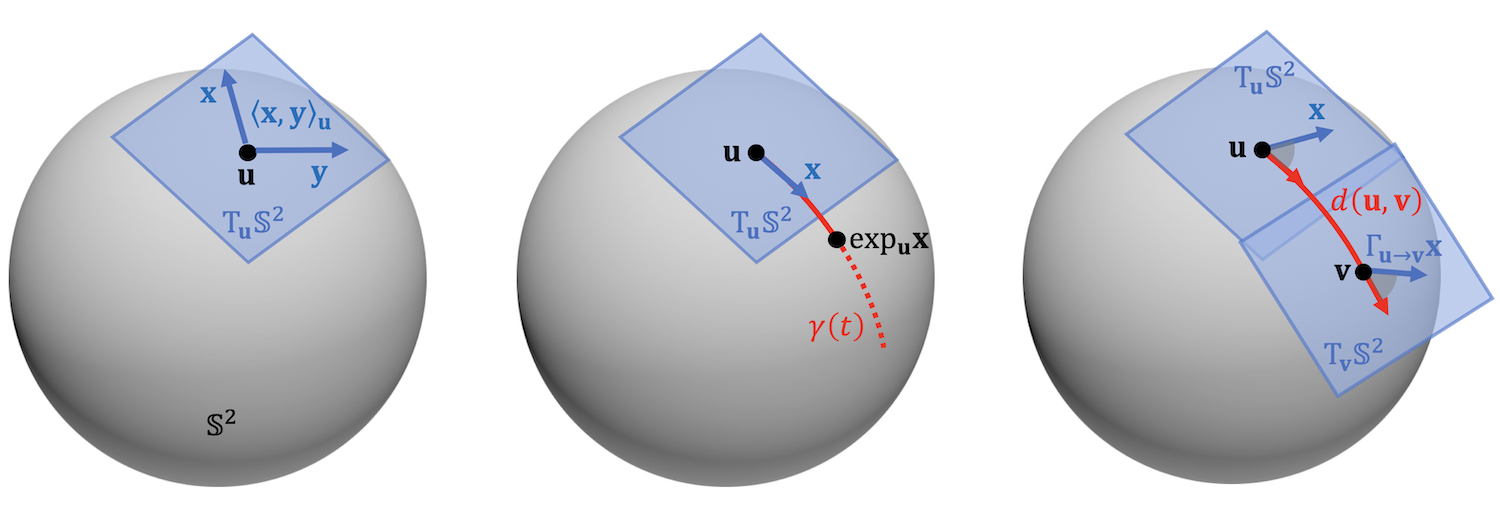
\includegraphics[width=\linewidth]{figures/manifold.png}
    \caption{
    以二维球面 $\mathbb{S}^2 = \{\mathbf{u}\in \mathbb{R}^3 : \|\mathbf{u}\|=1 \}$ 为例说明 Riemann 几何的基本概念；该球面实现为 $\mathbb{R}^3$ 的子集（子流形）。
%
球面的切空间为 $T_\mathbf{u}\mathbb{S}^2 = \{ \mathbf{x}\in \mathbb{R}^3 : \mathbf{x}^\top \mathbf{u} = 0\}$，它是二维平面，因此球面是二维流形。Riemann 度量就是限制在切平面上的 Euclidean 内积，即 $\langle \mathbf{x}, \mathbf{y}\rangle_\mathbf{u} = \mathbf{x}^\top \mathbf{y}$，对任意 $\mathbf{x},\mathbf{x}\in T_\mathbf{u}\mathbb{S}^2$ 成立。
指数映射为
$\exp_\mathbf{u}(\mathbf{x}) = \cos(\| \mathbf{x}\|)\mathbf{u} + \frac{\sin(\| \mathbf{x}\|)}{\|\mathbf{x}\|} \mathbf{x}$，其中 $\mathbf{x} \in T_\mathbf{u}\mathbb{S}^2$。
%
测地线是长度为 $d(\mathbf{u},\mathbf{v}) = \cos^{-1}(\mathbf{u}^\top \mathbf{v})$ 的大圆弧。
    }
    \label{fig:sphere_metric}
\end{figure}%


%an {\em inner product}.
%In differential geometry, an inner product on $T_u\Omega$ depending smoothly on $u$ is called a {\em Riemannian metric}, in honour of Bernhardt Riemann who introduced the concept in 1856. %
%We will denote a Riemannian metric as a$g_u: T_u\Omega \times T_u\Omega \rightarrow \mathbb{R}$ that allows to measure length, angle, and volume in the tangent space. 
%

%
%of a vector $$
%
%angle between two tangent vectors $x,y \in T_u\Omega$, (expressed %as $\cos^{-1}\left( \frac{\g_u(x,y)$) and a length of the 


配备度量的流形称为
{\em Riemann 流形}，完全能够用度量表达的性质称为{\em 内蕴性质}。%
这是本书讨论中的关键概念，因为按照我们的模板，将寻求构造作用于 $\Omega$ 上所定义信号的函数，使其对保持度量的变换具有不变性。这类变换称为{\em 等距变换}，它们使流形发生形变而不影响其局部结构。\marginnote{
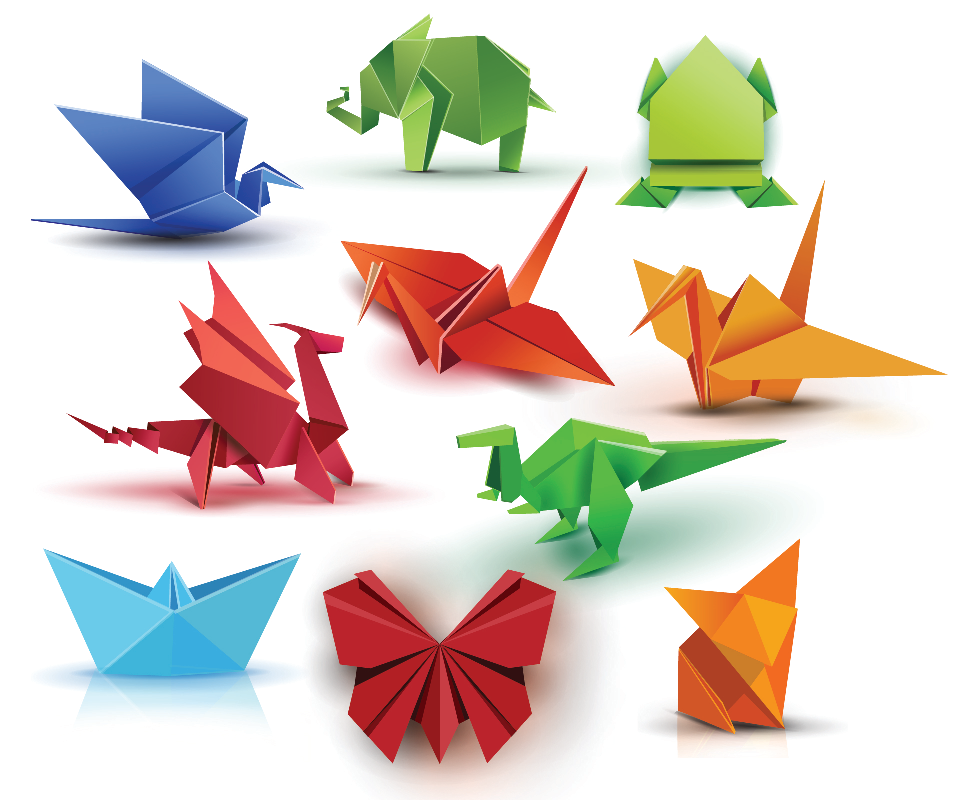
\includegraphics[width=1\linewidth]{figures/origami.pdf}
这一结果称为{\em 嵌入定理}，由
\cite{nash1971imbedding}.
%John Forbes Nash, who became a household name after the Hollywood movie The Beautiful Mind. 
折纸%paper folding
艺术体现了平面曲面在 $\mathbb{R}^3$ 中的不同等距嵌入（图片：Shutterstock/300 librarians）。
}如果这类函数能够用内蕴量表达，就会自动保证等距不变性，从而不受等距形变影响。
%
这些结果还可以进一步推广到近似等距变换；因而这是蓝图中所讨论几何稳定性（域形变）的一个实例。


%\taco{Taco: here we should probably make clear that we are not talking about symmetries in the sense of automorphisms, i.e. maps $\Omega \rightarrow \Omega$ that preserve the metric, but about isomorphisms, i.e. maps $\Omega \rightarrow \Omega'$ that preserve the metric. Note that we do not yet discuss this in the template, but as discussed we should.} 

%\michael{Approx isometry - geometric stability}

正如前面所指出的，Riemann 流形的定义不要求它
在任何空间中具有几何实现；但事实证明，任意光滑 Riemann 流形都可以实现为足够高维 Euclidean 空间的子集（此时称它“嵌入”该空间），并利用 Euclidean 空间的结构诱导 Riemann
度量。不过，这类嵌入未必唯一——正如下文将看到的，同一个 Riemann 度量可以具有两个不同的等距
实现。
%called {\em isometries}.



%\joan{Consider a transition paragraph here, where we explain that we introduce the minimal elements of differential geometry that lead to the key notion of isometry and geodesics}



\paragraph{标量场与向量场}
%
由于我们关心定义在 $\Omega$ 上的信号，需要给出流形上标量值
%\marginnote{We will use the same notation for tangent and vector fields, the distinction between which will be clear from the context.} 
与向量值函数的恰当概念。
%
（光滑）{\em 标量场}是形如 $x: \Omega\rightarrow \mathbb{R}$ 的函数。\marginnote{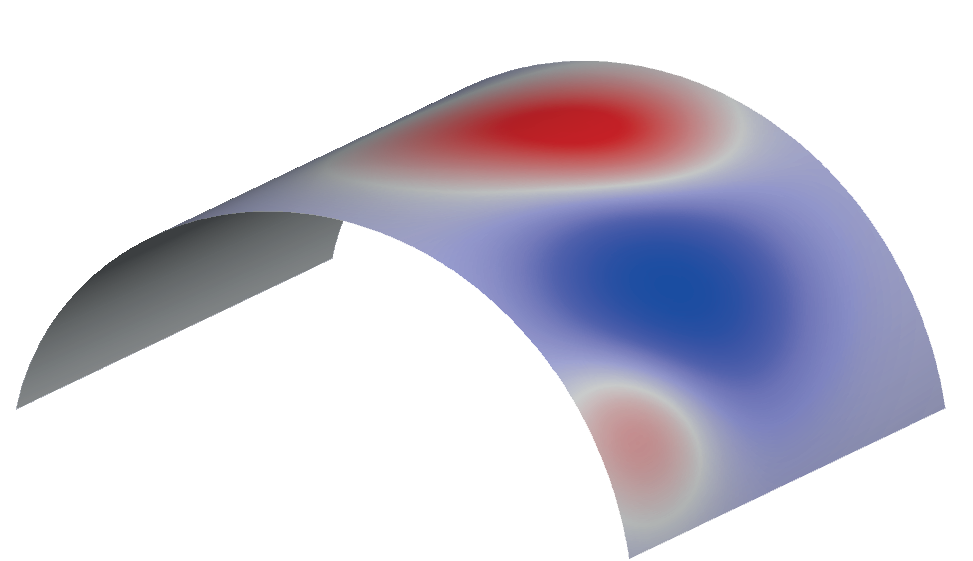
\includegraphics[width=0.9\linewidth]{figures/field_scalar.pdf}\\
标量场示例。
}
%\marginnote{The fields are typically assumed to be of the same regularity class (smoothness) as the manifold itself. }
%
%scalar-valued function  (often called a {\em scalar field}) $x: \Omega\rightarrow \mathbb{R}$ on the manifold. The space of 
标量场构成向量空间 $\mathcal{X}(\Omega, \mathbb{R})$，该空间可以配备内积%of scalar fields
\begin{equation}
\langle x, y \rangle = \int_\Omega x(u) y(u) \mathrm{d}u,
\label{eq:inner_scalar}   
\end{equation}
%
其中 $\mathrm{d}u$ %= \sqrt{\det g}$
%\marginnote{More rigorously speaking, the volume form requires an inner product (i.e. Riemannian metric) and {\em orientation} (`handedness'). } 
是由 Riemann 度量诱导的体积元素。
%
%
（光滑）{\em 切向量场}是形如 $X: \Omega \rightarrow T\Omega$ 的函数，它为每个点指定相应切空间中的一个切向量，即 $u\mapsto X(u)\in T_u\Omega$。
%
向量场\marginnote{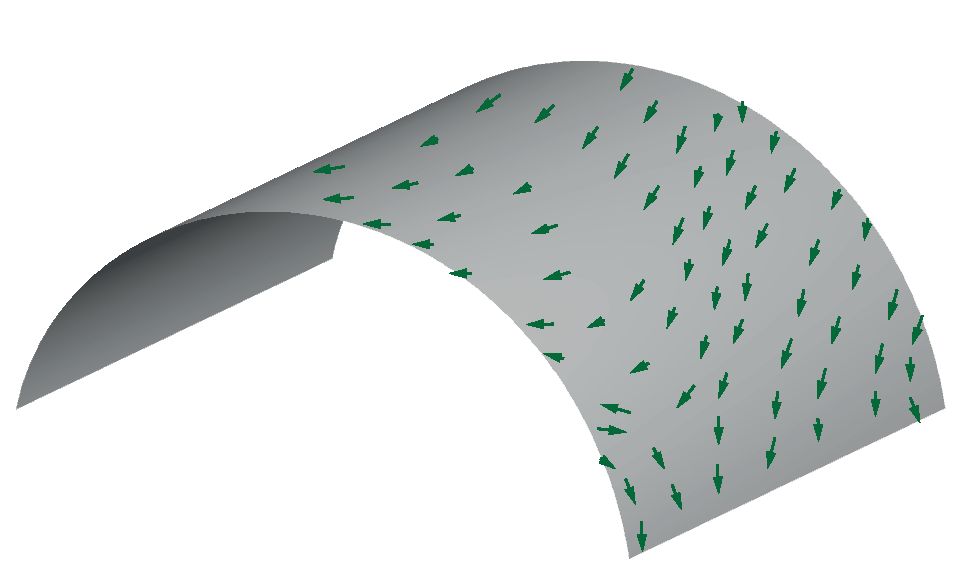
\includegraphics[width=0.9\linewidth]{figures/field_vector.pdf}\\
向量场示例。通常假设场与流形本身具有相同的正则性类别（光滑度）。
}也构成向量空间 $\mathcal{X}(\Omega, T\Omega)$，其内积由 Riemann 度量定义：
%
\begin{equation}
\langle X, Y \rangle = \int_\Omega g_u(X(u), Y(u)) \mathrm{d}u. \label{eq:inner_vector}   
\end{equation}


\paragraph{内蕴梯度}
理解（并实际{\em 定义}）向量场的另一种方式，是把它视为导数概念的推广。
%
在经典微积分中，可以通过{\em 微分} $\mathrm{d}x(u) = x(u+\mathrm{d}u) - x(u)$ 对（光滑）函数作局部线性化；它给出函数 $x$ 在点 $u$ 处因无穷小位移 $\mathrm{d}u$ 而发生的值变化。
%
然而，在本情形下无法直接套用这一定义，因为
%brings up two problems: First, 
由于缺乏全局向量空间结构，形如“$u+\mathrm{d}u$”的表达式在流形上没有意义。
%, preventing us from adding or subtracting two points on $\Omega$. 
%
%
%A second problem arises when trying to take derivatives of vector fields, as one would need to subtract vectors belonging to tangent spaces at {\em different points}, while subtraction is only define \emph{within} a single vector space. 





解决办法是%to the first problem is
用切向量对局部无穷小位移建模。
%in order to provide a proper generalization of the differential on manifolds. 
%
给定光滑标量场 $x\in \mathcal{X}(\Omega,\mathbb{R})$，可以把（光滑）向量场视为满足{\em 导子}性质的线性映射 $Y:\mathcal{X}(\Omega,\mathbb{R}) \rightarrow \mathcal{X}(\Omega,\mathbb{R})$：
$Y(c) = 0$ 对任意常数 $c$ 成立（对应于常数函数的导数为零这一直觉）；$Y(x+z) = Y(x) + Y(z)$（线性性）；以及 $Y(xz) = Y(x)z + xY(z)$（{\em 乘积法则}或 {\em Leibniz 法则}）。这些性质对任意光滑标量场 $x,z \in \mathcal{X}(\Omega,\mathbb{R})$ 均成立。
%
可以证明，能够利用这些性质公理化地定义向量场。
%
微分 $\mathrm{d}x(Y) = Y(x)$
可以视为算子 $(u,Y) \mapsto Y(x)$，
%
%defined as an operator $\mathrm{d}x : T\Omega \rightarrow \mathbb{R}$ of the form
%$$
%\mathrm{d}x(Y) = Y(x),
%$$
%which can be 
其解释如下：$x$ 因位移 $Y \in T_u\Omega$ 在点 $u$ 处而发生的变化，由 $\mathrm{d}_ux(Y)$ 给出。\marginnote{重要的是，这一构造{\em 完全不使用 Riemann 度量}，因此可以推广到第~\ref{sec:gauges} 节所讨论的更一般丛构造。}
%
因此，它是经典{\em 方向导数}概念的推广。
%



另一种观点是，在每个点 $u$ 处，可以把微分视为{\em 线性泛函} $\mathrm{d}x_u : T_u\Omega \rightarrow \mathbb{R}$，它作用于切向量 $X \in T_u\Omega$。向量空间上的线性泛函称为{\em 对偶向量}或{\em 余向量}；若还给定内积（Riemann 度量），则对偶向量总可以表示为
$$
\mathrm{d}x_u (X)  = g_u(\nabla x(u), X).\marginnote{This is a consequence of the Riesz-Fr{\'e}chet Representation Theorem, by which every dual vector can be expressed as an inner product with a vector. } 
$$ 
点 $u$ 处微分的表示是切向量 $\nabla x(u) \in T_u \Omega$，称为 $x$ 的（内蕴）{\em 梯度}；与经典微积分中的梯度类似，可以把它理解为 $x$ 增长最快的方向。
%
把梯度视为{\em 算子} $\nabla : \mathcal{X}(\Omega,\mathbb{R}) \rightarrow \mathcal{X}(\Omega,T\Omega)$ 时，它在每个点指定 $x(u) \mapsto \nabla x(u) \in T_u \Omega$；因此，标量场 $x$ 的梯度是向量场 $\nabla x$。
%As we will see later, this construction will allow us to generalise the notion of Fourier transform to manifolds. 

%More generally, the gradient can be thought of as an operator $\nabla : $



%In other words, the gradient produces a tangent vector field indicating the local direction of steepest increase of a scalar field on the manifold. 





%\taco{I think the notion of Torsion will be difficult to understand for newbies. Also, we are differentiating a tensor field g which I think we have not explained yet.

%We could consider just mentioning the LC connection and explaining that parallel transport defined wrt it will not change the length of tangent vectors. We can also say that if another condition (Torsion free) is satisfied, there is a unique LC connection, without formalizing it.}



\paragraph{测地线}

现在考虑流形上的光滑曲线 $\gamma : [0,T] \rightarrow \Omega$，其端点为 $u = \gamma(0)$ 和 $v = \gamma(T)$。曲线在点 $t$ 处的导数是切向量 $\gamma'(t) \in T_{\gamma(t)}\Omega$，称为{\em 速度向量}。\marginnote{默认假设曲线采用{\em 弧长参数化}，使得 $\| \gamma' \| = 1$（速度恒定）。}
%
在连接点 $u$ 与 $v$ 的所有曲线中，我们关心{\em 长度最短}的曲线，即寻找使长度泛函最小的 $\gamma$：
%
$$
\ell(\gamma) = \int_{0}^T \| \gamma'(t) \|_{\gamma(t)} \mathrm{d}t =  \int_{0}^T g_{\gamma(t)}^{1/2} (\gamma'(t), \gamma'(t)) \mathrm{d}t. 
$$
%
这类曲线称为{\em 测地线}（源自希腊语 \textgreek{geodai\textsigma{}{\'i}a}，字面意为“划分地球”），在微分几何中起着重要作用。
%
%
对本书讨论至关重要的是，我们对测地线的定义是内蕴的，因为它们只依赖 Riemann 度量（通过长度泛函）。


熟悉微分几何的读者可能记得，测地线是一个更一般的概念，其定义实际上未必需要 Riemann 度量，而只需要{\em 联络}（也称为{\em 协变导数}，因为它把导数概念推广到向量场和张量场）；联络与前面对微分的构造类似，以公理方式定义。
%
给定 Riemann 度量，存在唯一的特殊联络，称为\marginnote{Levi-Civita 联络无挠且与度量相容。Riemann 几何基本定理保证其存在性与唯一性。}{\em Levi-Civita 联络}；Riemann 几何通常默认使用该联络。由这一联络产生的测地线，就是上面定义的长度最短曲线。


下面将说明如何利用测地线定义在流形上传输切向量的方式（平行输运），建立从流形到切空间的局部内蕴映射（指数映射），并定义距离（测地度量）。这将允许我们通过在切空间中局部应用滤波器，构造类似卷积的运算。%
%among all curves with endpoints $u = \gamma(0)$ and $v=\gamma(T)$. 



\paragraph{平行输运}\marginnote{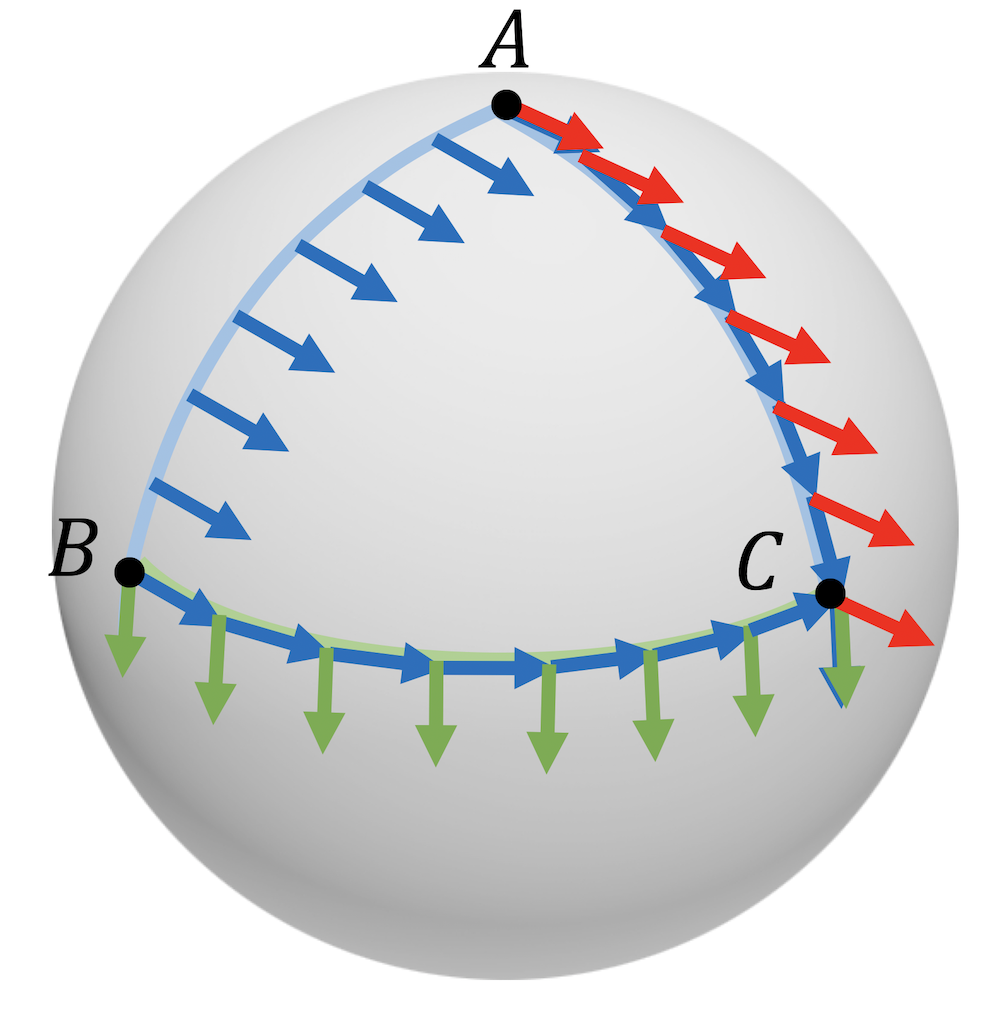
\includegraphics[width=0.9\linewidth]{figures/parallel.png}
在球面上，把向量从 A Euclidean 式地传输到 C 没有意义，因为所得向量（红色）不在切平面内。从 A 到 C 的平行输运（蓝色）沿路径旋转向量。它依赖于路径：沿 BC 与 ABC 路径输运会产生不同结果。
}
处理流形时已经遇到一个问题：不能直接对两点 $u,v \in \Omega$ 作加减运算。
%
比较不同点处的切向量时也会出现同样的问题：尽管维数相同，它们却属于{\em 不同空间}，例如 $X\in T_u\Omega$ 和 $Y\in T_v\Omega$，因而不能直接比较。
%
测地线提供了一种把向量从一点移动到另一点的机制，具体如下：令 $\gamma$ 为连接点 $u=\gamma(0)$ 与 $v=\gamma(T)$ 的测地线，并令 $X \in T_u\Omega$。可以沿测地线定义一组新的切向量 $X(t) \in T_{\gamma(t)}\Omega$，使 $X(t)$ 的长度以及它与曲线速度向量之间的夹角（由 Riemann 度量表示）保持不变：
$$
g_{\gamma(t)}(X(t),\gamma'(t) ) = g_{u}(X,\gamma'(0)) = \mathrm{const}, \quad\quad \|X(t)\|_{\gamma(t)} = \|X\|_u = \mathrm{const}.
$$
于是，在终点处得到唯一向量 $X(T) \in T_{v}\Omega$，该终点为 $v$。%, which is unique.


用上述记号定义的映射 $\Gamma_{u\rightarrow v}(X) : T_u\Omega \rightarrow T_u\Omega$ 和 $T_v\Omega$，即 $\Gamma_{u\rightarrow v}(X) = X(T)$，称为{\em 平行输运}或{\em 联络}；后一个术语意味着它是在切空间 $T_u\Omega$ 与 $T_v\Omega$ 之间建立“联结”的机制。
%
由于保持角度和长度，平行输运只相当于旋转向量，因此可与特殊正交群 $\mathrm{SO}(s)$ 的一个元素相关联（该群称为切丛的{\em 结构群}）。\marginnote{这里假设流形可定向，否则应为 $\mathrm{O}(s)$。}我们把该元素记为 $\fg_{u\rightarrow v}$，并将在第~\ref{sec:gauges} 节更详细地讨论。

如前所述，联络可以独立于 Riemann 度量以公理方式定义，从而给出沿任意光滑曲线进行平行输运的抽象概念。不过，这类输运的结果取决于所取路径。
%As a general comment, parallel transport can be defined along any cur

%or {\em connection} 




\paragraph{指数映射}
在点 $u$ 的局部，总能沿给定方向 $X \in T_u\Omega$ 定义唯一测地线，即满足%a smooth curve $\gamma_X : [0,T] \rightarrow \Omega$ satisfying
$\gamma(0) = u$ and $\gamma'(0) = X$. %, for some small $T>0$. 
%
%
当 $\gamma_X(t)$ 对所有 $t\geq 0$ 都有定义时（即可以从点 $u$ 出发把测地线延伸任意长），称流形{\em 测地完备}，且指数映射定义在整个切空间上。
%
由于紧致流形是测地完备的，可以默认采用这一便利性质。



%
这种由一点和一个方向定义测地线的方式，给出了从切空间 $T_u \Omega$（的一个子集）到 $\Omega$ 的自然映射，称为{\em 指数映射}。\marginnote{
%Here, $B_\delta(0)$ is a ball of radius $\delta$ around the origin. 
注意，测地完备性未必保证 $\exp$ 是全局微分同胚——最大半径 $r$ 以 $u$ 为中心，并使 $\exp_u(B_r(0) \subseteq T_u\Omega)$ 保持微分同胚映射；该半径称为{\em 单射半径}。}该映射为 $\exp : B_r(0) \subset T_u\Omega \rightarrow \Omega$，其定义是在方向 $X$ 上沿测地线前进一步，即 $\exp_u(X) = \gamma_X(1)$。%
%
指数映射 $\exp_u$ 是局部微分同胚，因为它把 $B_r(0)$（半径为 $r$ 的球，即 $T_u\Omega$ 中原点的邻域）形变为 $u$ 的一个邻域。反过来，也可以把指数映射视为流形到切空间的内蕴局部形变（“展平”）。




\paragraph{测地距离}
%
称为 Hopf-Rinow 定理的结果
%
\marginnote{因此，Hopf-Rinow 定理建立了测地完备性与度量完备性的等价性；后者意味着每个 Cauchy 序列都在测地距离度量下收敛。}保证测地完备流形也是{\em 完备度量空间}；在这样的空间中，任意点对 $u,v$ 之间的距离（称为{\em 测地距离}或{\em 度量}）都可以实现为连接两点的最短路径长度：
$$
d_g(u,v) = \min_{\gamma} \ell(\gamma) \quad\quad \text{s.t.} \quad\quad \gamma(0) = u, \,\, \gamma(T) = v,
$$
该路径存在（即最小值能够取到）。\marginnote{注意，“度量”一词有两种含义：Riemann 度量 $g$ 与距离 $d$。为避免混淆，指后者时将使用“距离”一词。记号 $d_g$ 表明距离依赖于 Riemann 度量 $g$，这种依赖通过测地长度 $L$ 的定义实现。}



%The term `geodesic' is also used in metric geometry, where it is defined as the shortest path. In the setting described here the two meanings coincide. }


%i.e., the two notions of `geodesic' used somewhat differently in differential and metric geometry







\paragraph{等距变换}
现在考虑把流形 $\Omega$ 形变为另一个流形 $\tilde{\Omega}$，后者配备 Riemann 度量 $h$；我们假设该形变是
%
%We will assume this map to be 
流形之间的微分同胚 $\eta: (\Omega, g) \rightarrow (\tilde{\Omega}, h)$。
%
其微分 $\mathrm{d}\eta : T\Omega \rightarrow T\tilde{\Omega}$ 定义了相应切丛之间的映射（称为{\em 前推}），使得
%\marginnote{The pushforward is what is called a {\em bundle map}.}
在点 $u$ 处有 $\mathrm{d}\eta_u : T_u \Omega \rightarrow T_{\eta(u)}\tilde{\Omega}$，%which allows to interpret it as follows:
%
其解释与前面类似：
如果用切向量从点 $u$ 作一个小位移，所用切向量为 $X \in T_u \Omega$，那么映射 $\eta$ 将从点 $\eta(u)$ 沿切向量 $\mathrm{d}\eta_u(X) \in T_{\eta(u)}\tilde{\Omega}$ 位移。


由于前推\marginnote{前推与拉回是伴随算子 $\langle \eta^* \alpha, X \rangle = \langle \alpha, \eta_*X \rangle$，其中 $\alpha \in T^*\Omega$ 是{\em 对偶向量场}，在每一点定义为作用于 $T_u\Omega$ 的线性泛函；两个内积分别定义在向量场和对偶向量场上。}提供了关联两个流形上切向量的机制，因而可以把度量 $h$ 从 $\tilde{\Omega}$ {\em 拉回}到 $\Omega$：
$$
(\eta^*h)_u(X,Y) = h_{\eta(u)}(\mathrm{d}\eta_u(X), \mathrm{d}\eta_u(Y))
$$ 
%
如果拉回度量在每一点都与 $\Omega$ 的度量一致，即 $g = \eta^*h$，则映射 $\eta$ 称为（Riemann）{\em 等距变换}。% (metric-preserving).
%
对于二维流形（曲面），等距变换可以直观地理解为非弹性形变：它使流形发生形变，却不“拉伸”或“撕裂”流形。



根据定义，等距变换保持测地距离等内蕴结构，而这些结构完全由 Riemann 度量表达。% and Gaussian curvature.
%
因此，也可以从度量几何的视角理解等距变换，
把它看作{\em 度量空间之间}保持距离的映射（“度量等距”）$\eta : (\Omega, d_g) \rightarrow (\tilde{\Omega}, d_h)$，即
$$
d_g (u,v) = d_h(\eta(u),\eta(v)) 
$$
对所有 $u,v \in \Omega$ 均成立，
更紧凑地写为 $d_g = d_h \circ (\eta \times \eta)$。换言之，Riemann 等距变换也是度量等距变换。
%
在{\em 连通}流形上，反之亦然：每个度量等距变换也是 Riemann 等距变换。
\marginnote{这一结果称为 Myers–Steenrod 定理。我们默认假设所讨论的流形是连通的。}
%where $d_g, d_g$ are the geodesic distances induced by the respective Riemannian metrics $g, h$. 


在几何深度学习蓝图中，$\eta$ 是域形变的模型。当 $\eta$ 为等距变换时，%(roughly, an inelastic deformation that does not `stretch' the manifold),
任何内蕴量都不受这类形变影响。
%
%This is the reason why we insist on working with structures defined intrinsically. 
%
可以通过下述概念推广精确的（度量）等距变换：%this notion
{\em 度量伸缩}
$$
\mathrm{dil}(\eta) = \sup_{u\neq v \in \Omega}\frac{d_h(\eta(u),\eta(v))}{d_g (u,v)}
$$
%
或{\em 度量畸变}
$$
\mathrm{dis}(\eta) = \sup_{u, v \in \Omega}|d_h(\eta(u),\eta(v)) - d_g (u,v)|,
\marginnote{The Gromov-Hausdorff distance
%\marginnote{
%More precisely, $d_{\mathrm{GH}}(\Omega,\Omega') = \frac{1}{2}\inf_{(x,y) \in C} %\mathrm{dis}$
%} 
between metric spaces, which we mentioned in Section~\ref{sec:isomorphism}, can be expressed as the smallest possible metric distortion.}
$$
它们分别刻画测地距离在 $\eta$ 作用下的相对变化与绝对变化。
%
函数 $f \in \mathcal{F}(\mathcal{X}(\Omega))$ 在域形变下保持稳定的条件~（\ref{eqn:domain_def_stability}）
在本情形下
可以重写为
$$
\| f(x,\Omega) - f(x\circ \eta^{-1},\tilde{\Omega})\| \leq C \|x\| \mathrm{dis}(\eta). 
$$


%[Gauss Theorema Egregium, definition of curvature through perimeter defect, pizza example]


\paragraph{内蕴对称性}
上述情形的一个特例是域自身的微分同胚（即第~\ref{sec:isomorphism} 节所称的{\em 自同构}），记为 $\tau \in \mathrm{Diff}(\Omega)$。若拉回度量满足 $\tau^* g = g$，则称其为 Riemann\mbox{（自）等距变换}；若 $d_g = d_g\circ (\tau \times \tau)$，则称其为度量（自）等距变换。
%
不出所料，\marginnote{流形上的连续对称性由特殊切向量场无穷小地生成，这类场称为{\em Killing 场}，以 Wilhelm Killing 命名。}等距变换在复合运算下构成群，记为 $\mathrm{Iso}(\Omega)$，称为{\em 等距群}；其恒等元素是映射 $\tau(u) = u$，逆元素总是存在（因为 $\tau$ 按定义为微分同胚）。
%
因此，自等距变换是流形的{\em 内蕴对称性}。


%Continuous symmetries on manifolds are infinitesimally generated
%%\marginnote{More correctly, Killing fields are the infinitesimal generators of continuous symmetries. } 
%by special tangent vector fields called {\em Killing fields}, named after Wilhelm Killing. A field $X$ is Killing if the  Lie derivative\marginnote{The Lie derivative in this case is a derivative of forms. For scalar and vector fields, it coincides with the covariant derivative $\mathcal{L}_X y = \nabla_X y$ and the commutator $\mathcal{L}_X Y = [X,Y]$, respectively. } of the Riemannian metric along it vanishes, $\mathcal{L}_X g = 0$, which is interpreted as 
%%
%$$
%\mathcal{L}_X g(Y,Z) = g(\nabla_Y X, Z) + g(Y,\nabla_Z X) = 0
%$$
%for any smooth tangent fields $Y, Z$. 
%%
%We can recap that like we mentioned in Section~\ref{sec:symmetries}, we can regard symmetries as automorphisms (self-maps) preserving additional structure: either the local Riemannian metric, or global geodesic distances between pairs of points. 
%%\taco{Do we need Killing fields? It's interesting but I worry that we'd need to properly introduce Lie derivatives to make it understandable.} \michael{Lets keep them for now}
%%OK :)



\paragraph{流形上的 Fourier 分析}
%Reconnecting to our Geometric Deep Learning blueprint, we now have a way to guarantee geometric stability by construction, considering intrinsic quantities expressed through the Riemannian metric. 
%
下面说明如何在流形上构造内蕴的类卷积运算；按照构造，这些运算对等距形变具有不变性。
为此，
%In order to define convolution-like operations, 
有两种选择：其一是类比 Fourier 变换，把卷积定义为 Fourier 域中的乘积。
%
其二是在空间域定义卷积，即把滤波器与信号作局部相关。
%by ``shifting'' a filter around via parallel transport.
先讨论谱方法。


回顾一下，在 Euclidean 域中，Fourier 变换由循环矩阵的特征向量得到；循环矩阵由于可交换而能够同时对角化。因此，任意循环矩阵，特别是微分算子，都可以用于在一般域上定义 Fourier 变换的类比。
%
在 Riemann 几何中，通常使用 Laplacian 算子的正交特征基；下面给出其定义。


为此，回顾内蕴梯度算子 $\nabla : \mathcal{X}(\Omega,\mathbb{R}) \rightarrow \mathcal{X}(\Omega,T\Omega)$ 的定义；
%assigning at each point $x(u) \mapsto \nabla x(u) \in T_u \Omega$. In other words, the gradient produces 
它产生一个切向量场，指示流形上标量场局部增长最快的方向。
%
类似地，可以定义{\em 散度算子} $\nabla^* : \mathcal{X}(\Omega,T\Omega) \rightarrow \mathcal{X}(\Omega,\mathbb{R})$。
%
若把切向量场视为流形上的
流，散度就度量该场在一点处的
净流量，从而能够区分场的
“源”和“汇”。
%
我们使用记号 $\nabla^*$（而非常见的 $\mathrm{div}$），以强调这两个算子互为伴随：
$$
\langle X, \nabla x\rangle = \langle \nabla^* X,  x\rangle,
$$
其中使用标量场与向量场上的内积（\ref{eq:inner_scalar}）和~（\ref{eq:inner_vector}）。
%with the inner products defined on vector and scalar fields, respectively. 

{\em Laplacian}（在微分几何中也称为 {\em Laplace-Beltrami 算子}）是定义在 $\mathcal{X}(\Omega)$ 上的算子：$\Delta = \nabla^* \nabla$，
%; as opposed to most of the textbooks, we use the negative sign to ensure our operator is positive semi-definite. 
%
其解释为\marginnote{由这一解释还可清楚看出 Laplacian 是各向同性的。第~\ref{sec:meshes} 节将看到，可以定义形如 $\nabla^*(A(u)\nabla)$ 的{\em 各向异性 Laplacian}（见 \citep{andreux2014anisotropic,boscaini2016anisotropic}），其中 $A(u)$ 是决定局部方向的、依赖于位置的张量。
%In practice, such a construction requires a fixed gauge. 
}
%For the classical Euclidean Laplacian defined as the sum of second-order derivatives this can be seen by writing it as the trace of the Hessian, $\Delta x(\mathbf{u})= \mathrm{trace} \nabla^2 x(\mathbf{u})$, applying an orthogonal transformation of coordinates $\mathbf{u}\mapsto \mathbf{Ru}$,  and using the chain rule.
%}
一点周围无穷小球面上的函数平均值
与函数在该点自身取值
之差。
%
%
它是数学物理中最重要的算子之一，用于描述热扩散、量子振荡、
波传播等多种现象。
%
对本书而言，重要的是 Laplacian 具有内蕴性，因而在 $\Omega$ 的等距变换下保持不变。



容易看出 Laplacian 是自伴（“对称”）的：
$$
\langle \nabla x, \nabla x \rangle = \langle x , \Delta x\rangle = \langle \Delta x ,  x\rangle.
$$
上式左侧的二次型实际上就是已经熟悉的 Dirichlet 能量：
$$c^2(x) = \| \nabla x \|^2 = \langle \nabla x, \nabla x \rangle = \int_\Omega \| \nabla x(u) \|_u^2 \mathrm{d}u = \int_\Omega g_u( \nabla x(u),  \nabla x(u)) \mathrm{d}u
$$
它度量 $x$ 的光滑性。
%As we will see in the following, the Laplacian plays a center role in signal processing and learning on non-Euclidean domains, as its eigenfunctions generalize the classical Fourier bases, allowing to perform spectral analysis on manifolds and graphs
%
%
%
%
%allowing to interpret it as the smoothest orthogonal basis. 
%
%
%We will discuss this construction in detail in Chapter ???, where we will show that Laplacian eigenvalues and eigenvectors capture important geometric properties of the manifold. 



Laplacian 算子具有特征分解%eigenfunctions
$$
\Delta \varphi_k = \lambda_k \varphi_k, \quad\quad k=0, 1, \hdots 
$$
%
%which is discrete 
若流形紧致（我们默认如此），其谱可数；其特征函数相互正交，即 $\langle \varphi_k, \varphi_l \rangle = \delta_{kl}$，这是由于 $\Delta$ 自伴。
%discrete on compact manifolds
%orthogonal since $\Delta$ is self-adjoint
%
Laplacian 特征基也可以构造为 Dirichlet 能量的一组正交极小化子：
$$
\varphi_{k+1} = \arg\min_{\varphi} \| \nabla \varphi \|^2      \quad\quad \text{s.t.}\quad\quad   \|\varphi \|=1 \,\,\, \text{and} \,\,\, \langle \varphi, \varphi_{j} \rangle = 0 
$$
其中 $j=0,\hdots, k$；因此可以把它理解为 $\Omega$ 上最光滑的正交基。
%
特征函数 $\varphi_0, \varphi_1, \hdots$ 与对应特征值 $0 = \lambda_0 \leq \lambda_1 \leq \hdots $，可以分别理解为经典 Fourier 变换中原子与频率的类比。\marginnote{事实上，$e^{\mi \xi u}$ 是 Euclidean Laplacian $\tfrac{\mathrm{d}^2}{\mathrm{d} u^2}$ 的特征函数。}
%


利用这一正交基，可以把 $\Omega$ 上的平方可积函数展开为{\em Fourier 级数}：
$$
x (u) = \sum_{k \geq 0} \langle x, \varphi_k \rangle \varphi_k (u)
$$
%
其中 $\hat{x}_k = \langle x, \varphi_k \rangle$ 称为{\em Fourier 系数}，也称为 $x$ 的（广义）Fourier 变换。\marginnote{注意，由于 $\Omega$ 的紧致性使谱离散，这一 Fourier 变换具有离散索引。}
%
截断 Fourier 级数会产生逼近误差，\citep{aflalo2013spectral} 给出的上界为
$$
\left\| x - \sum_{k = 0}^N \langle x, \varphi_k \rangle \varphi_k \right\|^2 \leq \frac{\| \nabla x\|^2}{\lambda_{N+1}}.
$$
\cite{aflalo2015optimality} 进一步表明，没有其他基能获得更小的误差，因此 Laplacian 特征基对于表示流形上的光滑信号是{\em 最优的}。


\paragraph{流形上的谱卷积}
%Let us now remind the reader that we defined Euclidean convolution in Section~\ref{sec:groups} as inner product with a shifted filter $(x \star \psi)(u) =  \langle x, T_u \psi \rangle$. This construction had two important properties, linearity and commutativity, that works in both ways, allowing to {\em define} convolution as a linear operator that commutes with shift. 
%%
%On a manifold, because we lack a global vector space structure, we cannot immediately define the shift operator $(T_v x)(u) = x(u-v)$ since ``$u-v$'' makes no sense. 
%%
%However, we can keep $T_u$ as an abstract linear operator and use the above two properties as a definition. 
%
%
%First, we note that commutativity implies 
%$$
%(T_v (x\star \psi))(u) = \langle x, T_v T_u \psi \rangle =  \langle T_v x, T_u  \psi \rangle = ((T_v x)\star \psi)(u).  
%$$
%%
%Expressing each of the functions %$x$, $T_u \psi$, and $T_v x$ 
%in the Fourier basis allows us to rewrite %this identity as 
%\begin{eqnarray*}
%\langle T_v x, T_u\psi \rangle &=& \left \langle 
%\sum_{k\geq 0} \langle T_v x,\varphi_k \rangle \varphi_k \,, \,\,
%\sum_{l\geq 0} \langle T_u\psi,\varphi_l \rangle \varphi_l
%\right \rangle \\
%&=& \sum_{k,l\geq 0} \langle T_v x,\varphi_k \rangle \langle T_u\psi,\varphi_l \rangle \langle \varphi_k, \varphi_l \rangle \\
%&=& \sum_{k \geq 0} \langle T_v x,\varphi_k \rangle \langle T_u\psi,\varphi_k \rangle, \marginnote{We use here the orthogonality of the basis, $\langle \varphi_k, \varphi_l \rangle = \delta_{kl}$.}
%\end{eqnarray*}
%%
%and similarly, 
%$
%\langle x, T_v T_u\psi \rangle =
%\sum_{k \geq 0} \langle x,\varphi_k \rangle \langle T_v  T_u\psi,\varphi_k \rangle
%$,
%%
%from where the spectral expression of the commutativity condition follows:
%$$
%\langle T_v x,\varphi_k \rangle \langle T_u\psi,\varphi_k \rangle 
%= \langle x,\varphi_k \rangle \langle T_v  T_u\psi,\varphi_k \rangle \quad\quad \text{for all} \, k\geq 0.
%$$
%In particular, for $x=\psi = \varphi_l$ we get 
%$
%\langle T_v \varphi_l,\varphi_k \rangle \langle T_u \varphi_l,\varphi_k \rangle 
%= \delta_{kl} \langle T_v  T_u \varphi_l,\varphi_k \rangle 
%$
%which leads us to $\langle T_v \varphi_l,\varphi_k \rangle = 0$ for $k\neq l$. This means that Fourier basis functions are the eigenfunctions of the shift operator, like we had in the Euclidean case,  i.e., $T_v \varphi_k = \mu_v \varphi_k$.
%
%
%In order to determine the eigenvalues $\mu_v$, we consider again the commutativity condition with $x=\varphi_k$ and $\psi = \delta_u$ the Dirac delta function\marginnote{The {\em Dirac delta} or {\em impulse function} is defined as $\langle \delta_u , x \rangle = x(u)$. It can thus be considered as the representation of the linear functional (dual vector) $x \mapsto x(u)$.  } 
%
%
%
%Second, using  the linearity of $T_v$, we get 
%%the general expression  
%$$
%(T_v x)(u) = \sum_{k\geq 0} \langle x, \varphi_k\rangle (T_v \varphi_k) (u)
%= \sum_{k\geq 0} \langle x, \varphi_k\rangle  \varphi_k (v) \varphi_k (u)
%= \sum_{k\geq 0} \hat{x}_k  \varphi_k (v) \varphi_k (u), 
%%\marginnote{In the Euclidean case, one has (from the associativity of exponents and complex conjugation in the inner product) $\varphi_i (v) \bar{\varphi}_i (u) = \varphi_i (v - u)$. In the general case, the shift operator is thus position-dependent and the signal is {\em changed} when shifted.  }
%$$
%which is a non-Euclidean generalisation of the shift operator. 
%%
%It is easy to verify that in the Euclidean case, $\Omega = [0,L]$, \marginnote{ Here we assume a compact interval, in which case the Fourier basis is discrete. Note that the shift we get is $x(u+v)$ rather than $x(u-v)$, which is just notational difference.}  where the Fourier basis is of the form $\varphi_k(u) = e^{\mi \frac{2\pi k}{L} u}$, we get the familiar expression 
%$$
%(T_v x)(u) = \sum_{k\geq 0} \hat{x}_k e^{\mi \frac{2\pi k}{L} v} e^{\mi \frac{2\pi k}{L} u} 
%\sum_{k\geq 0} \hat{x}_k e^{\mi \frac{2\pi k}{L} (u+v)} = x(u+v).
%$$
%
%
%Finally, plugging the expression of $T_u$ into the definition of convolution, we get
%%{\em spectral convolution}
%%
%\begin{eqnarray}
%(x \star \psi)(u) &=& \langle x, T_u \psi \rangle = 
%\left \langle x, \, \sum_{k\geq 0} \hat{\psi}_k \varphi_k(u) \phi_k 
%\right\rangle \nonumber \\
%&=&
%\sum_{k \geq 0} \langle x, \varphi_k \rangle \hat{\psi}_k  \varphi_k (u)  = \sum_{k \geq 0} (\hat{x}_k \cdot \hat{\psi}_k ) \varphi_k (u).
%\label{eqn:conv_spectral}
%\end{eqnarray}
%%
%%In a sense, we used what was a {\em property} of the classical Fourier transform (the Convolution Theorem) as a way to {\em define} a non-Euclidean convolution. 
%%
%Expression~(\ref{eqn:conv_spectral}) is often called {\em spectral convolution}, since it coincides with the Convolution Theorem, expressing the convolution in spectral domain as the point-wise product of the Fourier transforms $\hat{\psi}_k$ and $\hat{x}_k$.  
%%
%This construction is usually motivated by using a {\em property} of the classical Fourier transform (the Convolution Theorem) as a way to {\em define} a non-Euclidean convolution. However, here we have shown the derivation from first principles of shift equivariance (where the shift is understood in a more general sense). 
%%
%The key property of spectral convolution is that, by virtue of its construction, it is intrinsic and thus isometry-invariant. 




{\em 谱卷积}可以定义为信号 $x$ 与滤波器 $\theta$ 的 Fourier 变换之积：
\begin{equation}
(x \star \theta)(u) = 
\sum_{k \geq 0} (\hat{x}_k \cdot \hat{\theta}_k ) \varphi_k (u).
\label{eqn:conv_spectral}
\end{equation}
%
注意，这里把经典 Fourier 变换的一项{\em 性质}（卷积定理）用作{\em 定义}非 Euclidean 卷积的方式。
%
根据构造，谱卷积具有内蕴性，因而具有等距不变性。
%
此外，由于 Laplacian 算子各向同性，它没有方向概念；在这一意义上，该情形类似于第~\ref{sec:proto-graphs} 节中的图，因为邻域聚合具有置换不变性。







\begin{figure}[h!]
    \centering
    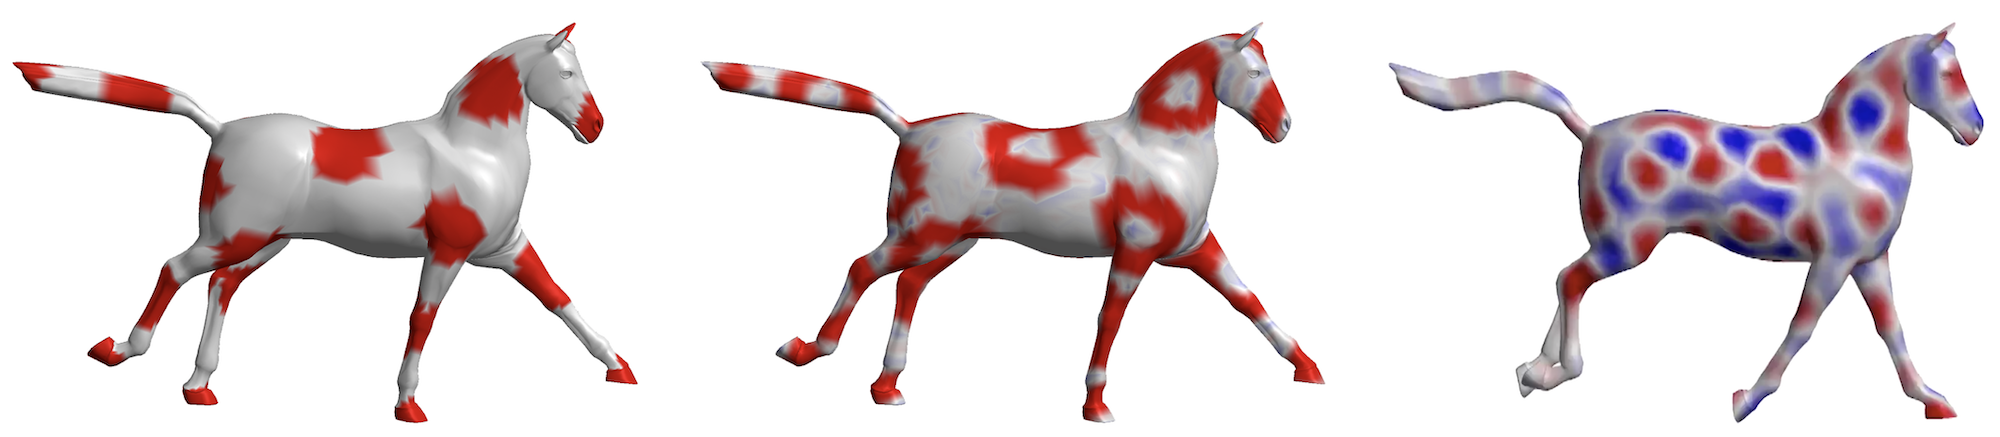
\includegraphics[width=\linewidth]{figures/horses.png}
    \caption{谱滤波器在域扰动下的不稳定性。左：信号 $\mathbf{x}$，位于网格 $\Omega$ 上。中：谱滤波结果%$\mathbf{x}\star \boldsymbol{\theta} = \boldsymbol{\Phi}\, \mathrm{diag}(\hat{\boldsymbol{\theta}}) \boldsymbol{\Phi}^\top \mathbf{x}$
    ，该结果位于%$\boldsymbol{\Phi}$
    Laplacian $\Delta$ 的特征基中，该算子定义在 $\Omega$ 上。
    右：
    同一个谱滤波器 %$\boldsymbol{\theta}$
    作用于%$\bar{\boldsymbol{\Phi}}$
    Laplacian $\tilde{\Delta}$ 的特征向量，该算子属于近似等距扰动域 $\tilde{\Omega}$，
    %(as a result of a near-isometric deformation of the mesh)  
%    $\bar{\boldsymbol{\Phi}}\, \mathrm{diag}(\hat{\boldsymbol{\theta}}) \bar{\boldsymbol{\Phi}}^\top \mathbf{x}$
    产生了截然不同的结果。
    }
    \label{fig:mesh_horses}
\end{figure}%




%
在实践中，由于需要对角化 Laplacian，直接计算~（\ref{eqn:conv_spectral}）的代价高得难以承受。更糟的是，
%, as we will see in Section~\ref{sec:meshes}, 
它在几何上并不稳定：即使域 $\Omega$ 只受到很小的近似等距扰动，Laplacian 的高频特征函数也可能发生显著变化（见图~\ref{fig:mesh_horses}）。
%
%
更稳定的解决方案是把滤波器实现为形如 $\hat{p}(\Delta)$ 的{\em 谱传递函数}：
%which is understood in the operator sense as %\marginnote{Geometric Deep Learning methods based on spectral convolution expressed through the Fourier transform are often referred to as `spectral' and opposed to `spatial' methods we have seen before in the context of graphs. When expressed as spectral transfer function, the former in fact boil down to the latter, so this dichotomy is somewhat artificial and not completely appropriate.}
\begin{eqnarray}
(\hat{p}(\Delta) x)(u) &=& \sum_{k\geq 0} \hat{p}(\lambda_k) \langle x, \varphi_k\rangle \varphi_k (u) \label{eqn:conv_spec} \\
%
&=& \int_\Omega x(v) \, \sum_{k\geq 0} \hat{p}(\lambda_k) \varphi_k(v) \varphi_k (u) \, \mathrm{d}v \label{eqn:conv_spat}
\end{eqnarray}
%
它可以有两种解释：一是解释为谱滤波器~（\ref{eqn:conv_spec}），其中令 $\hat{\theta}_k = \hat{p}(\lambda_k)$；二是解释为空间滤波器~（\ref{eqn:conv_spat}），其位置相关核为 $\theta(u,v) = \sum_{k\geq 0} \hat{p}(\lambda_k) \varphi_k(v) \varphi_k (u)$。
%
%
这种表述的优点是，$\hat{p}(\lambda)$ 可以用少量系数参数化；选择多项式等参数函数\marginnote{基于通过 Fourier 变换表达的谱卷积之几何深度学习方法，常称为“谱”方法，并与此前在图语境下看到的“空间”方法相对。这里可以看出，这两种观点可能等价，因此这种二分有些人为，并不完全恰当。}$\hat{p}(\lambda) = \sum_{l=0}^r \alpha_l \lambda^l$ 后，可以高效地把滤波器计算为
$$
(\hat{p}(\Delta) x)(u) = \sum_{k\geq 0} \sum_{l= 0}^r \alpha_l \lambda_k^l \, \langle x, \varphi_k\rangle \varphi_k (u) = \sum_{l= 0}^r \alpha_l (\Delta^l x)(u),
$$
从而完全避免谱分解。
%
第~\ref{sec:meshes} 节将更详细地讨论这一构造。

%\michael{Add note on stability}

%While filters defined in this manner are isotropic (direction-unaware), 



\paragraph{流形上的空间卷积}

第二种选择是尝试通过在不同点匹配滤波器来定义流形上的卷积，就像式~（\ref{eq:group-conv}）中所做的那样：
%
\begin{equation}
(x \star \theta)(u) = \int_{T_u \Omega} x(\exp_u Y) \theta_u(Y) \mathrm{d}Y, 
\label{eq:conv_tangent_space}
\end{equation}
%
其中，现在必须使用指数映射从切空间访问标量场 $x$ 的值，并且
滤波器 $\theta_u$ 定义在每一点的切空间中，因而依赖于位置。%
如果以内蕴方式定义滤波器，这类卷积就具有等距不变性；前文已指出，这一性质在许多计算机视觉与图形学应用中至关重要。
%, and we use the exponential map to obtain. 


不过，需要注意它与第~\ref{sec:grids_euclidean}--\ref{sec:groups} 节此前构造之间的几个实质区别。
%
第一，由于流形通常不是齐性空间，不再具有允许共享滤波器的全局群结构；所谓共享，是指使用相同的 $\theta$ 于每个 $u$，而不是使用 $\theta_u$ 于式~（\ref{eq:conv_tangent_space}）中。因此，不能在一点定义滤波器后再将其移动到各处。
%as we did in formula~(\ref{eq:group-conv}). 
%
在流形上类比这一运算需要平行输运，使共享滤波器 $\theta$（定义为 $T_u\Omega$ 上的函数）能够应用于另一个 $T_v\Omega$。
%
然而，正如前面所见，这通常取决于 $u$ 与 $v$ 之间的路径，因此{\em 移动滤波器的方式很重要}。%\marginnote{As a possible remedy, \cite{poulenard2018multi} suggested moving the filter along geodesics. }
%
%
第三，由于指数映射只能在局部使用，滤波器必须是{\em 局部的}，其支撑受单射半径限制。
%
第四，
也是最关键的一点，不能直接使用 $\theta(X)$，因为 $X$ 是抽象几何对象；为了用于计算，必须把它{\em 相对于某个局部基}表示出来，
该局部基为 $\omega_u : \mathbb{R}^s \rightarrow T_u\Omega$，所得表示是 $s$ 维坐标数组 $\mathbf{x} = \omega^{-1}_u(X)$。
%
由此可以把卷积~（\ref{eq:conv_tangent_space}）重写为
%
\begin{equation}
(x \star \theta)(u) = \int_{[0,1]^s} x(\exp_u (\omega_u \mathbf{y})) \theta(\mathbf{y}) \mathrm{d}\mathbf{y}, 
\label{eqn:conv_exp}
\end{equation}
%

%\joan{We have used $\delta$ in the previous sections to refer to the size of the filter support}

其中滤波器定义在单位立方体上。由于指数映射是内蕴的（通过测地线定义），所得卷积具有等距不变性。


然而，这里默认假设可以把标架 $\omega_u$ 一同带到另一个流形，即 $\omega_u' = \mathrm{d}\eta_u \circ \omega_u$。
%
%Yet, we should point to one issue that at a close inspection opens a can of worms: in our definition, we assumed $\omega$ was given, which 
不过，仅给定流形 $\Omega$ 时，要以一致方式获得
这样的标架（物理学术语称为\emph{规范}）困难重重。
%implies that we need some mechanism to {\em fix a basis at each point} of the manifold (in physics, a smooth choice of local bases is referred to as a {\em gauge}). 
%
第一，光滑全局规范可能不存在：对于不可\emph{平行化}的流形就是如此。\marginnote{球面 $\mathbb{S}^2$ 是不可平行化流形的一个例子；这一结论源自
%on which one cannot construct a smooth tangent vector field. 
{\em Poincar{\'e}-Hopf 定理}，通俗地说就是“无法在不产生发旋的情况下梳平一个毛球”。\vspace{2mm}
%and is the reason why magnetic plasma confinement chambers must have toroidal rather than spherical geometry. 
%\includegraphics[width=1\linewidth]{figures/hairy_ball.png}
}在这种情况下，无法定义处处非零的光滑切向量场。
%; we further assume that the global gauge is smooth, which is only possible if the manifold is {\em parallelizable}.
%
%
第二，流形上不存在典范规范，因此这种选择具有任意性；由于卷积依赖于 $\omega$，选择不同规范会得到不同结果。

应当指出，这是实践与理论相背离的情形：在实践中，
%one can get around these mathematical issues in a somewhat satisfactory manner.
%That is, 
%there exist algorithms that will 
可以构造大部分区域光滑、仅含有限个奇点的标架，例如取流形上某个内蕴标量场的内蕴梯度。\marginnote{
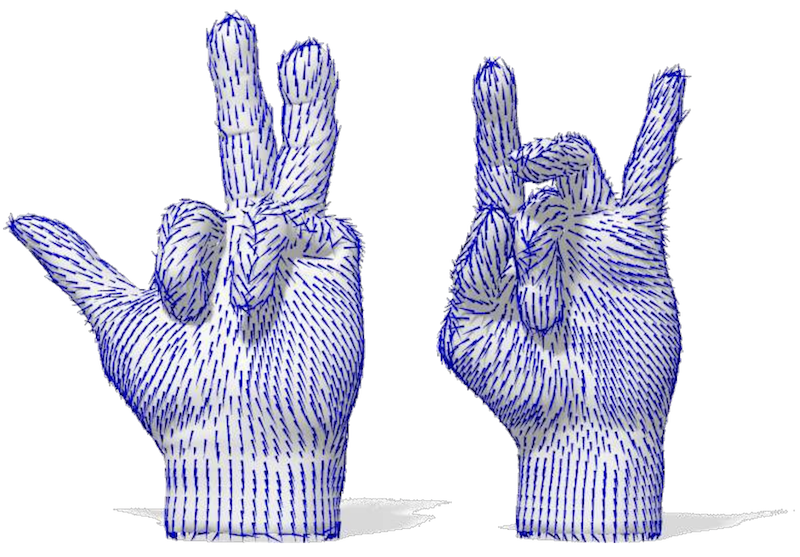
\includegraphics[width=1\linewidth]{figures/gframes.png} 
使用 GFrames 算法 \cite{melzi2019gframes} 在近似等距流形上构造稳定规范的例子（仅显示一个轴）。
} 
%(such as e.g. the North and South pole of the sphere in the sidebar), for instance taking the two frame vectors to correspond to the highest and least curved direction on a 2D manifold. 
%
此外，这类构造具有稳定性，即以这种方式构造的标架在等距流形上相同，在近似等距流形上相似。
%
事实上，早期流形深度学习工作已经采用这类方法 \citep{masci2015geodesic,monti2017geometric}。
%the same frame is found for isometric manifolds, and for nearly isometric ones a similar frame is found. 


不过，这一解决方案并不完全令人满意，因为在奇点附近，滤波器方向（以相对于规范的固定方式定义）会剧烈变化，导致即使输入信号与滤波器光滑，特征图仍不光滑。
%
此外，没有明确理由说明为何点 $u$ 处的某一方向应被视为等价于完全不同点 $v$ 处的另一方向。
%
因此，尽管存在{\em 实用的}替代方案，下面仍将寻找
%methods based on semi-intrinsic frames can be useful, 
一种在{\em 理论上}更有依据、并且完全不依赖规范选择的方法。
%which we will discuss next. 
%We will discuss just such an approach next.


%\joan{This is still a bit long, but already much improved from earlier versions. 
%One aspect that is still not very explicit is how to precisely connect with the GDL blueprint, in terms of the composition of local equivariant maps, and global invariant map. 
%Here we argue that differential operators such as the Laplacian are defined intrinsically (isometry invariant), and thus any representation that is based on it will preserve this isometric invariance. Equivariance in this context is less obvious (equivariance with respect to changes in the gauge, parametrisation/charting?).

%Also, should we mention stability of the Laplacian to metric deformations? How to ensure that the information we extract from the Laplacian is not too unstable? we can mimic the discussion from previous section on wavelet vs fourier, to illustrate that the high-frequency eigenfunctions of the laplace-beltrami  are unstable. THis is mentioned in the mesh section, should it be restated here as well?
%}

%
%
%Assume now we have some vector-valued data $\Omega$. 
%In differential geometry, this is modelled as a {\em vector field} $x:\Omega \rightarrow T\Omega$, assigning to each point $u \in \Omega$ a tangent vector $x(u) \in T_u \Omega$. 
%%
%%
%%The reason we need to consider gauges is that we can only describe geometric data numerically \emph{relative to a gauge}.
%%
%Relative to a gauge, we can express each tangent vector as a coordinate vector, i.e. an array of numbers, and so a vector field becomes a map $\mathbf{x} : \Omega \rightarrow \R^{s}$.
%%
%In other words, we can, as previously, think of vector fields as signals forming the space $\mathcal{X}_{\R^s}(\Omega)$ with the inner product 
%%(\ref{eqn:innerprod}) [Only well defined if we choose a metric? Should we assume Riemannian manifolds?]. 
%$$
%\langle x, y\rangle = 
%\int_\Omega  \langle x(u), y(u) \rangle_{T_u\Omega} du = 
%\int_\Omega \mathbf{x}^\top(u) \mathbf{G}(u) \mathbf{y}(u) du,  
%$$
%%
%where $\mathbf{G}$ is the representation of the {\em Riemannian metric} (defined as an inner product on $T_u\Omega$ depending smoothly on $u$) in the same local frame.
%%

%As in the examples discussed in previous sections, this group can act via different representation $\rho$, which in this case corresponds to different kinds of fields, including scalar fields, vector fields, tensor fields, each of which is characterized by how it transforms under a change of gauge.



%\paragraph{Local Symmetries and Spatial Weight Sharing}


% ----
% OLD:

% Let us start from the simplest case of {\em scalar fields}, i.e. signals $\mathcal{X}(\Omega, \mathbb{R})$. 
% %




% Importantly, not only the {\em features} change when we change the gauge, also the {\em network layers} depend on the choice of gauge. 
% %
% Consider an architecture in the spirit of `message passing' we saw in graph neural networks, where at each point $u\in \Omega$, we aggregate the transformed feature vectors from neighbor points $v$, 
% and 
% %
% for simplicity, assume this transformation is linear. 
% %
% When the vectors are expressed w.r.t. a gauge, this transformation takes the form of matrix multiplication  $\mathbf{A}(u,v)\mathbf{x}(v)$; this notation emphasizes the fact that the matrix can be different for each pair of points $u, v$.  
% %.\marginnote{What we describe here is the GCN architecture. In attentional architectures, we can have $\mathbf{A}(\mathbf{x}(u),\mathbf{x}(u'))$ rather than $\mathbf{A}(u, u')$. }
% %
% %Note however an crucial difference: on a graph, the matrix $\mathbf{A}$ must be {\em the same} for all points $u'$, as this is needed for permutation equivariance. 
% %
% %In the case of a manifold, there is no such a global symmetry, so we can use a different matrix $\mathbf{A}(u,u')$ for each pair of (neighbor) points. 



% If we perform a gauge transformation, the input feature vector changes as $\mathbf{x}(u) \mapsto \rho(\fg(u)) \mathbf{x}(u)$, and the output feature should change as $\mathbf{x}(v) \mapsto \rho(\fg(v)) \mathbf{x}(v)$\marginnote{We assume here for simplicity that the input and output features are of the same type and thus have the same representation $\rho(\fG)$.}.
% It follows that we should change $\mathbf{A}(u,v) \mapsto \rho(\fg(v)) \mathbf{A}(u,v) \rho(\fg(u))^{-1}$.
% Although the new weight matrix and feature vectors contain different numbers, the underlying geometric objects are mapped in the same way regardless of the gauge.



% % Gauge equivariant message; 
% If gauge transformations are considered as symmetries, a network layer, and hence an individual message, should be equivariant to gauge transformations.
% That is, the weight matrix $A_{uu'}$ should satisfy $\rho(g(u'))^{-1} A_{uu'} = A_{uu'} \rho(g(u))$ for all gauge transformations $g : \Omega \rightarrow \fG$.
% This is an extremely strong constraint, because $g(u)$ and $g(u')$ (the gauge transformation at $u$ and $u'$) can vary independently.
% As a consequence the weight matrix $A_{uu'}$ is so constrained that it cannot learn very interesting mappings.

% % Connection
% The solution is to introduce an additional piece of structure called a \emph{connection}, which relates the feature spaces at $u$ and $u'$. % via parallel transport (see Figure TODO).
% The connection gives us for any two nearby points $u, u'$ a straightest curve (geodesic) between them, and a notion of \emph{parallel transport} of frames and feature vectors along this curve (see Figure TODO).
% %The parallel transporter from $u$ to $u'$ along a geodesic is an element of $\fG$ denoted $\fg_{u \rightarrow u'} \in \fG$ that transforms as $\fg_{u \rightarrow u'} \mapsto \fg(u') \fg_{u \rightarrow u'} \fg(u)^{-1}$ under a gauge transformation $\fg(u)$.
% Using parallel transport, we can move the feature vector $v_u$ at $u$ to $u'$, before applying the weight matrix $A_{uu'}$.
% Since this matrix maps input features at $u$ to output features at $u$, it only has to deal with the gauge at $u$.
% In other words, it should satisfy a more conventional equivariance constraint: $A_{uu'} \rho(g(u)) = \rho(g(u)) A_{uu'}$ that only involves $g(u)$ and not $g(u')$. \michael{[TACO: isn't it the other way around, you transport vectors from u' to u?]}

% % Spatial weight sharing; filter on tangent plane; identify tangent planes via gauge;
% What we have seen so far is that gauge symmetries constrain the weight matrix $A_{uu'}$, but that the weight matrices associated with different points need not necessarily share weights as in a convolution layer.




%In each of the examples discussed so far, we started with a space $\Omega$ and a group of symmetries $\fG$ acting on it.
%In some cases however, e.g. when the domain $\Omega$ is a general manifold or mesh, it may not have any obvious symmetries.
%%For instance, if $\Omega$ is a general manifold, it may not have any non-trivial symmetries.
%In this case, we cannot define an action of $\fG$ on the space of signals on $\Omega$ and use it to slide filters around to define a convolution.
%Nevertheless, in this example as many others, there is still a group of symmetries lurking beneath the surface, but this is an altogether kind of symmetry known as \emph{gauge symmetry}.
%
%The word gauge here refers to a choice of frame (ordered basis) for a vector space, or more generally to one such choice for each vector space in a collection of vector spaces $V_u$ associated with the points $u \in \Omega$.
%For example, if we have a manifold $\Omega$, we can construct the \emph{tangent bundle} $T \Omega$ which consists of a collection of vector spaces $T_u \Omega$ (the tangent spaces), one for each point in $u \in \Omega$ (see Figure TODO).
%So in this example a gauge is a choice of frame for each of the tangent spaces $T_u \Omega$.\marginnote{
%We note that in mathematical gauge theory one would require the gauge to be smooth, in which case a globally defined gauge may not always exist. We will ignore these subtleties and not insist on smoothness.
%}
%
%The reason we need to consider gauges is that we can only describe geometric data numerically \emph{relative to a gauge}.
%Let's imagine our data consists of a vector field on $\Omega$.
%A vector field assigns to each point $u \in \Omega$ a tangent vector $v \in T_u \Omega$.
%Relative to a gauge, we can express each tangent vector as a coordinate vector, i.e. a list of numbers, and so a vector field becomes a map $x : \Omega \rightarrow \R^{n}$ (where $n$ is the dimension of the manifold and tangent spaces).
%In other words, our input space is $\mathcal{X}(\Omega, \R^n)$.
%However it is important to realize that what we are really interested in is the underlying geometrical object (vector field), whose representation as a function $x \in \mathcal{X}(\Omega, \R^n)$ depends on the choice of gauge.
%%However there is no canonical choice of gauge, so depending on our choice we will get different coordinate vectors.
%
%When we change the gauge, there is at each position a unique invertible matrix that maps the old gauge to the new one.
%In other words, a gauge transformation is a mapping $g : \Omega \rightarrow \GL{n}$, where $\GL{n}$ is the group of invertible $n \times n$ matrices.
%We can also restrict our attention to e.g. right-handed orthogonal frames, which are related by rotations, in which case a gauge transformation is a map $g : \Omega \rightarrow \SO{n}$ assigning to each position a rotation.
%In general, one considers a group $\fG$ (called the structure group) and a collection of frames such that for any two of them there is a unique $\fg \in \fG$ that maps one frame onto the other.
%As in the examples discussed in previous sections, this group can act via different representation $\rho$, which in this case corresponds to different kinds of fields, including scalar fields, vector fields, tensor fields, each of which is characterized by how it transforms under a change of gauge.
%
%% Associated bundles / reps of G
%% In the previous sections on Graphs, Grids and Groups, we discussed how the same group may act on various feature spaces through different representations $\rho$.
%% In the case of gauge transformations the same is true: we can define various kinds of fields such as scalar, vector, and tensor fields, by choosing an appropriate representation $\rho$ of the structure group $\fG$.
%% For instance, a scalar field (e.g. surface temperature on earth) does not depend on the frame (a scalar does not have a direction), so it corresponds to the trivial representation $\rho_0(g) = 1$.
%% A 2-tensor field would transform as $A_u \mapsto \fg A_u \fg^T$, where $u \in \Omega$, $A_u \in \R^{n \times n}$ and $\fg \in \fG$ is the change of basis matrix relating two gauges.
%
%%Given two vector fields, we can take at each position the outer (tensor) product $v w^T$ to obtain a tensor field, which tra
%
%% Gauge equivariant message from u to v; need for a connection / parallel transport
%%If gauge transformations are considered as symmetries, a network layer should be equivariant to gauge transformations.
%Not only the features change when we change the gauge, also the network layers depend on the choice of gauge.
%We will consider a message passing layer, and focus first on a single message sent from $u \in \Omega$ to $u' \in \Omega$.
%In a graph neural network, one would take the feature vector $v_u$ at $u$ and multiply it by a weight matrix $A$ to get the feature vector $v_{u'}$ at $u'$, before summing over all neighbours $u'$.
%The same weight matrix is used for all pairs of adjacent points $u,u'$, because this is required for equivariance to permutations.
%In the case of a manifold, we don't have such a global symmetry, so we are free to use a different matrix $A_{uu'}$ for each pair of (nearby) points $u, u'$.
%Now if we perform a gauge transformation, the input feature changes as $v_u \mapsto \rho(g(u)) v_u$, and the output feature should change as $v_{u'} \mapsto \rho(g(u')) v_{u'}$\marginnote{We assume here that the input and output feature are of the same type, i.e. have the same representation $\rho$ of $\fG$.}.
%It follows that we should change $A_{uu'} \mapsto \rho(g(u')) A_{uu'} \rho(g(u))^{-1}$.
%Although the new weight matrix and feature vectors contain different numbers, the underlying geometric objects are mapped in the same way regardless of the gauge.
%
%% Gauge symmetries / gauge equivariance
%To say that gauge transformations are symmetries is to say that any two gauges related by a gauge transformation are to be considered equivalent. %, and that data expressed relative to these frames should be processed in the same way regardless of the gauge.
%For instance, if we take $\fG = \SO{n}$, any two right-handed orthogonal frames are considered equivalent, because we can map any such frame to any other such frame.
%In other words, there is are no distinguished local directions such as ``up'' or ``right''.
%Similarly, if $\fG = \Orth{n}$, then any left and right handed orthogonal frame are considered equivalent.
%In this case, there is no preferred orientation either.
%
%% Gauge equivariant message; 
%If gauge transformations are considered as symmetries, a network layer, and hence an individual message, should be equivariant to gauge transformations.
%That is, the weight matrix $A_{uu'}$ should satisfy $\rho(g(u'))^{-1} A_{uu'} = A_{uu'} \rho(g(u))$ for all gauge transformations $g : \Omega \rightarrow \fG$.
%This is an extremely strong constraint, because $g(u)$ and $g(u')$ (the gauge transformation at $u$ and $u'$) can vary independently.
%As a consequence the weight matrix $A_{uu'}$ is so constrained that it cannot learn very interesting mappings.
%
%% Connection
%The solution is to introduce an additional piece of structure called a \emph{connection}, which relates the feature spaces at $u$ and $u'$. % via parallel transport (see Figure TODO).
%The connection gives us for any two nearby points $u, u'$ a straightest curve (geodesic) between them, and a notion of \emph{parallel transport} of frames and feature vectors along this curve (see Figure TODO).
%%The parallel transporter from $u$ to $u'$ along a geodesic is an element of $\fG$ denoted $\fg_{u \rightarrow u'} \in \fG$ that transforms as $\fg_{u \rightarrow u'} \mapsto \fg(u') \fg_{u \rightarrow u'} \fg(u)^{-1}$ under a gauge transformation $\fg(u)$.
%Using parallel transport, we can move the feature vector $v_u$ at $u$ to $u'$, before applying the weight matrix $A_{uu'}$.
%Since this matrix maps input features at $u$ to output features at $u$, it only has to deal with the gauge at $u$.
%In other words, it should satisfy a more conventional equivariance constraint: $A_{uu'} \rho(g(u)) = \rho(g(u)) A_{uu'}$ that only involves $g(u)$ and not $g(u')$.
%
%% Spatial weight sharing; filter on tangent plane; identify tangent planes via gauge;
%What we have seen so far is that gauge symmetries constrain the weight matrix $A_{uu'}$, but that the weight matrices associated with different points need not necessarily share weights as in a convolution layer.
%
%----
%
%% Spatial weight sharing; filter on tangent plane; identify tangent planes via gauge;
%What we have seen so far is that gauge symmetries constrain the weight matrix $A_{uu'}$, but that the weight matrices associated with different points need not necessarily share weights as in a convolution layer.
%In order to share weights across spatial locations, we need to somehow identify local patches around each point in $\Omega$.
%A popular approach is based on the observation that these local patches can first be identified with the tangent planes $T_u \Omega$ via the exponential map (see Figure TODO). %, so that we can write $A_{uu'}$ instead as $A_{uv}$ where $v \in T_u \Omega$ is a tangent vector that satisfies $u' = \exp_u(v)$.
%Furthermore, the tangent spaces themselves can be identified with $\R^n$ through the choice of a gauge.
%Hence, we can define the filter as a matrix-valued function $A$ on $\R^n$ (which parameterizes the neighbour $u'$) and which is independent of $u$.
%
%Since the filter is now tied to the gauge, it will be rotated when we rotate the gauge.
%Hence, the equivariance constraint becomes $A(g v) = \rho(g) A(v) \rho(g)^{-1}$.
%
%Thus, we can define a gauge equivariant convolution of a field $x$ on $\Omega$ and a filter $A$ as follows:
%\begin{equation}
%    (x \star A)(u) = \int_{\R^n} A(v) \, \rho(\fg_{\exp_u(v) \rightarrow u}) \, x(\exp_u(v)) dv,
%\end{equation}
%where $\exp_u(v)$ denotes the neighbour $u'$ indexed by $v \in \R$ and $\fg_{\exp_u(v) \rightarrow u} \in \fG$ denotes the parallel transport from this neighbour to $u$.
%



%---


% If gauge transformations are considered as symmetries, a mapping (network layer) $f : \mathcal{X}(\Omega, \R^n) \rightarrow \mathcal{X}(\Omega, \R^m)$ should be equivariant to gauge transformations.
% As a first example, consider a $1 \times 1$ convolution, i.e. $f$ consists of applying a linear map $\psi : \R^n \rightarrow \R^m$ at each position $u \in \Omega$.
% The input feature vector $v_u \in \R^n$ is a coordinate vector defined relative to some choice of gauge, and we will want that the output feature vector $w_u = \psi(v_u)$ is expressed relative to the same gauge.
% If we change the gauge by $g_u \in \fG$, then the input transforms as $v_u \mapsto \rho_{\textup{in}}(g_u) v_u$ and the output should transform by $w_u \mapsto \rho_{\textup{out}}(g_u) w_u$.
% Hence we $\psi$ should be equivariant: $\psi \circ \rho_{\textup{in}}(g_u) = \rho_{\textup{out}}(g_u) \circ \psi$ for all $g_u \in \fG$.

% The example of a $1 \times 1$ convolution is simple, because the input and output feature vectors $v_u$ and $w_u$ have the same spatial position $u \in \Omega$, and hence are represented with respect to the same gauge.
% In a general convolution, one would sum/integrate the messages sent from points $u'$ near $u$ as well, using a learned map $\psi_{uu'} : \R^n \rightarrow \R^m$.
% For this function we would have the constraint $\psi_{uu'} \circ \rho_{\textup{in}}(g_{u'}) = \rho_{\out}(g_u) \circ \psi_{uu'}$.
% However, since $g_u$ and $g_{u'}$ can vary independently (we can freely change the gauge at each position separately), this is an overly constraint and any $\psi_{uu'}$ that satisfies it will be uninteresting.

% The remedy is to introduce an object called a \emph{connection} that tells us how to compare feature vectors at $u$ and feature vectors at $u'$.
% That is, we take a map $c_{u \rightarrow u'} : \R^n \rightarrow \R^n$ 
% [TBC...]

%[Discuss internal symmetries.]

% In the context of geometric deep learning, the vector space in question is $\mathcal{C}$, i.e. the feature vector space that is attached to each position in $\Omega$ to build the space $\mathcal{X}(\Omega, \mathcal{C})$ of signals $x : \Omega \rightarrow \mathcal{C}$.


% The word gauge here refers to a choice of frame (ordered basis) for a vector space.
% In the context of geometric deep learning, the vector space in question is $\mathcal{C}$, i.e. the feature vector space that is attached to each position in $\Omega$ to build the space $\mathcal{X}(\Omega, \mathcal{C})$ of signals $x : \Omega \rightarrow \mathcal{C}$.
% Consider for now just a single copy of $\mathcal{C}$.
% We know from linear algebra that a linear map $f : \mathcal{C} \rightarrow \mathcal{C}$ can be expressed as a matrix $A$ if we choose a frame for $\mathcal{C}$, and likewise a vector $V \in \mathcal{C}$ can be represented as a coordinate vector $v \in \R^n$.
% If we change the frame, the matrix representation of $f$ changes as $A \mapsto P A P^{-1}$, where $P$ is called the change of basis matrix in linear algebra, or gauge transformation, in physics.
% The coordinate vector changes as $v \mapsto P v$.

% If we consider $P$ as a gauge \emph{symmetry}, then $A$ should be equivariant, i.e. $PA = AP$.
% Equivalently, we should have $A = PAP^{-1}$, i.e. $A$ has the same matrix representation in all frames related by a gauge symmetry.
% Hence, the matrix $A$ can be applied to coordinate vectors not just in one frame, but also to any other frame related by a gauge symmetry.
% For instance, if we consider the group of rotations as gauge symmetries, then any two orthogonal frames of the same handedness can be considered equivalent and $A$ can be applied to coordinate vectors in any such frame.
% Similarly, if we consider both rotations and reflections to be gauge symmetries, the same is true for orthogonal frames of different handedness.

% In gauge theory, this idea is generalized in two ways.
% Firstly, since we are dealing with signals $x : \Omega \rightarrow \mathcal{C}$, we have not just one vector space $\mathcal{C}$, but one copy of $\mathcal{C}$ associated with every point $u \in \Omega$.\marginnote{The vector space attached at $u \in \Omega$ is sometimes called the fibre $\mathcal{C}_u$ at $u$.}
% We are free to choose a different basis for each of these vector spaces, and so a general gauge transformation consists of one transformation at each point in $\Omega$.
% In other words, a gauge transformation is a function $g : \Omega \rightarrow \fG$, where $\fG$ is called the structure group (e.g. rotations or roto-reflections in the examples above).

% Secondly, as in the case of global symmetries acting on $\Omega$, one may consider different representations $\rho$ of the same group $\fG$ in each feature space in the network.
% Thus, if we have a representation $\rho$ of $\fG$ in $\mathcal{C}$, then a gauge transformation $g : \Omega \rightarrow \fG$ acts on a signal $x : \Omega \rightarrow \mathcal{C}$ as $x(u) \mapsto \rho(g(u)) x(u)$.  % todo check if we need an inverse on g?

% \taco{TODO: work on formatting of examples}
% \begin{tcolorbox}[width=\linewidth,
%                   boxsep=0pt,
%                   left=7.5pt,
%                   right=7.5pt,
%                   top=7.5pt,
%                   bottom=7.5pt,
%                   arc=0pt,
%                   boxrule=0pt,toprule=0pt,
%                   colback=boxgray,
%                   ]%%
%     Example: tangent vectors on a manifold.
    
%     Consider a smooth manifold $\Omega$ of dimension $2$.
%     % For instance, $\Omega$ could be an iso-energy surface of a protein [cite Michael's paper].
%     At each point $u \in \Omega$, there is a tangent space $T_u \Omega$ (see Figure TODO).
%     A \emph{vector field} is an assignment of a vector $v_u \in T_u \Omega$ to each point $u \in \Omega$.
%     If we choose a frame for each tangent space, we can express a vector field as a function $v : \Omega \rightarrow \R^2$.
%     ...
% \end{tcolorbox}


% \begin{tcolorbox}[width=\linewidth,
%                   boxsep=0pt,
%                   left=7.5pt,
%                   right=7.5pt,
%                   top=7.5pt,
%                   bottom=7.5pt,
%                   arc=0pt,
%                   boxrule=0pt,toprule=0pt,
%                   colback=boxgray,
%                   ]%%
%     Example: color space symmetry.
    
    
% \end{tcolorbox}


%Typically a problem comes with a fixed structure group $\fG$ and space $\Omega$, but the feature spaces $\mathcal{X}(\Omega, \mathcal{C}_l)$ at each layer $l$ may 

% the matrix $A$ can be applied to coordinate vectors in any equivalent basis; if $w = Av$ and we change the basis, $v' = P v$ then $w' = A P v = P A v = P w$.
% That is, if we apply $A$ to a coordinate vector relative some basis, we get an output coordinate vector relative to the same basis.



% To postulate a gauge symmetry is to postulate that frames related by certain kinds of gauge transformations are equivalent.
% For instance, two frames related by a rotation or reflection, can be considered equivalent.
% Or if we care about handedness, only those frames related by a rotation should be considered equivalent.



% Both global symmetries acting on $\Omega$ and gauge symmetries acting on $\mathcal{C}$ change how a signal is represented numerically, e.g. in computer memory.
% However, whereas global symmetries considered act on the domain $\Omega$, gauge symmetries act on the range $\mathcal{C}$ of signals $x : \Omega \rightarrow \mathcal{C}$.
% For example, in the case of graphs, a permutation will shuffle the node feature vectors but not change the feature vectors themselves.
% Conversely, a gauge transformation will change the feature vectors but not move them around on $\Omega$.


\subsection{规范与丛}
\label{sec:gauges}

我们已把规范定义为切空间的标架；不过，规范概念
%In the previous section we have already touched on the concept %of a gauge, defining it as a frame for the tangent space. 
%
%The notion of gauge as used in physics is however 
在物理学中一般得多：它可以指任意\marginnote{从历史上看，纤维丛最早出现在 {\'E}lie Cartan 的现代微分几何中（但他没有显式定义它们），随后在 20 世纪 30 年代的拓扑学中被进一步发展为独立对象。}\emph{向量丛}的标架，而不仅是切丛的标架。
%
非形式地说，向量丛描述由另一个空间参数化的一族向量空间，并且
由\emph{底空间} $\Omega$ 构成；底空间中每个位置都附着同一个向量空间 $\mathbb{V}$（称为\emph{纤维}），该位置为 $u \in \Omega$（对于切丛，纤维就是切空间 $T_u\Omega$）。
%and a continuous {\em projection function} $\pi : V \rightarrow \Omega$. 
%
粗略地说，丛在局部看起来像乘积 $\Omega \times \mathbb{V}$，这里所说的局部是点 $u$ 周围；但在全局上，丛可能发生“扭曲”，从而具有不同的整体结构。
%
%A {\em section} of the bundle is a 
%collection of identical vector spaces attached to the points in the manifold $\Omega$. 
%
%
%
%
在几何深度学习中，纤维%in question are
可用于对流形 $\Omega$ 中每一点的特征空间建模，纤维维数等于特征通道数。
在这一语境下，可能会出现一种新颖而迷人的对称性，称为\emph{规范对称性}。% \joan{Good opening. Can we give a concrete example of this symmetry? Physics application?}

%[Say something about setting? Assume manifold is known and the same for all data points. Each data point is a different signal on it. This is different from previous section where we assume manifold is different for each data point / manifold is part of the data.]


%\joan{Mobius strip}

%\joan{Field theory invariants -- ask Kyle for a nice example}
%Before we discuss the general case, 


再次考虑 $s$ 维流形 $\Omega$ 及其切丛 $T\Omega$，以及向量场
%consider again a vector field 
$X : \Omega \rightarrow T \Omega$（在这一术语中称为切丛上的一个{\em 截面}）。
%
相对于切丛的规范 $\omega$，$X$ 表示为函数 $\mathbf{x} : \Omega \rightarrow \R^s$。
不过，重要的是认识到我们真正关心的是底层几何对象（向量场）；它作为函数 $\mathbf{x} \in \mathcal{X}(\Omega,\R^s)$ 的表示{\em 依赖于规范的选择} $\omega$。
%
如果改变规范，也需要改变 $\mathbf{x}$，以保持其所表示的底层向量场不变。

%\michael{Give a comment from physics where this need arises: general relativity?}

%Likewise, we then need to change the layers of the network so that when they receive inputs expressed relative to the new gauge, they also produce outputs relative to that gauge; like a change of basis, but for many vector spaces at once.

% Taco: note, this itself is not gauge equivariance yet. Only if we *dont* need to change the map, yet it passes through gauge transformations, we have gauge equivariance.
%Since there is no `canonical' way to set a gauge, 
%we must ensure $x$ transforms appropriately when the gauge is changed -- a property we will call {\em gauge-equivariance}. 

%
%\begin{figure}[h!]
%    \centering
%    %\includegraphics{}
%    \caption{TODO: figure showing a manifold with a vector field on it, with one tangent plane drawn. In this tangent plane, a frame is drawn. The coordinates of the vector on that tangent plane is shown below. On the right, an identical figure but with a different frame, and different coordinates. Alternatively, we can draw a plane with a vector field on it. Then we dont draw tangent planes but we draw frames at regularly spaced intervals. The vector field is the same for the left and right figure, but the frame is different.}
%    \label{fig:into:vector-field-gauge}
%\end{figure}


%However there is no canonical choice of gauge, so depending on our choice we will get different coordinate vectors.

%\joan{Here we could already give a couple of examples. 
%
%}


\paragraph{切丛与结构群}
改变规范时，需要在每一点应用一个把旧规范映射到新规范的可逆矩阵。对每一点处的每一对规范，该矩阵都是唯一的，但在不同点处可能不同。
%
%\marginnote{We can also restrict our attention to e.g. right-handed orthogonal frames, which are related by rotations, in which case a gauge transformation is a map $\fg : \Omega \rightarrow \SO{s}$ assigning to each position a rotation.} 
换言之，{\em 规范变换}是映射 $\fg : \Omega \rightarrow \GL{s}$，其中 $\GL{s}$ 是由可逆 $s \times s$ 矩阵组成的{\em 一般线性群}。
它作用于规范 $\omega_u : \R^s \rightarrow T_u \Omega$，产生新规范 $\omega'_u = \omega_u \circ \fg_u : \R^s \rightarrow T_u \Omega$。
%
规范变换作用于坐标向量场%$\mathbf{x}$
的每一点，
通过 $\mathbf{x}'(u) = \fg^{-1}_u \mathbf{x}(u)$ 产生坐标表示 $\mathbf{x}'$，它相对于新规范表示 $X$。
%
底层向量场保持不变：
$$
X(u) = \omega'_u(\mathbf{x'}(u)) = \omega_u( \fg_u \fg^{-1}_u \mathbf{x}(u)) = \omega_u(\mathbf{x}(u)) = X(u), 
$$
这正是所期望的性质。
%
%
%
更一般地，可以考虑按照表示 $\rho$ 变换的几何量场，而该表示属于 $\GL{s}$；例如二阶张量（矩阵）场 $\mathbf{A}(u) \in \R^{s \times s}$，其变换方式为 $\mathbf{A'}(u) = \rho_2(\fg^{-1}_u) \mathbf{A}(u) = \rho_1(\fg_u) \mathbf{A}(u) \rho_1(\fg^{-1}_u)$。%\michael{The notation here is confusing: before we had $\rho$ as a matrix acting on vectors. Here it acts on both sides of $A$. Perhaps we should already mention the same thing when talking about graphs, where we have the representation of permutations acting on the adjacency matrix? }
%\taco{Decision: use $\mathbf{R}$ as the matrix representation of $\fg$}
在这种情形下，规范变换 $\fg_u$ 通过 $\rho(\fg_u)$ 作用。

有时可能只关注具有某种性质的标架，例如正交标架、右手标架等。
自然地，我们关心的是一组保持某种性质并构成群的变换。
例如，保持正交性的群是正交群 $\Orth{s}$（旋转与反射），而还保持定向或“手性”的群是 $\SO{s}$（纯旋转）。
因此，一般而言有一个称为丛之\emph{结构群}的群 $\fG$，规范变换则是映射 $\fg : \Omega \rightarrow \fG$。
关键观察是：在所有具有给定性质的情形下，对于给定点处的任意两个标架，恰有一个规范变换将它们联系起来。

%\taco{Introduce parallel transport here? Say it is $\fG$-valued}

如前所述，规范理论不局限于切丛；一般而言，可以考虑向量空间丛，其结构和维数未必与底空间 $\Omega$ 的结构和维数相关。\marginnote{我们用 $s$ 表示底空间 $\Omega$ 的维数，用 $d$ 表示纤维维数。对于切丛，$d=s$ 是底层流形的维数。对于 RGB 图像，$s=2$ 且 $d=3$。}
例如，彩色图像像素在二维网格上的位置为 $u \in \Omega = \Z^2$，在 RGB 空间中的取值为 $\mathbf{x}(u) \in \R^3$；因此，可以把像素空间视为一个向量丛，其底空间为 $\Z^2$，每一点附着纤维 $\R^3$。
%
通常相对于这样一种规范来表示 RGB 图像：该规范依次以 R、G、B 为基向量，因此图像的坐标表示为 $\mathbf{x}(u) = (r(u), g(u), b(u))^\top$。
也可以在每个位置独立置换基向量（颜色通道），只要记住每一点采用的标架（通道顺序）即可。\marginnote{在本例中，我们选择 $\fG = \Sigma_3$，即三个颜色通道的置换，作为丛的结构群。也可以采用其他选择，例如色相旋转 $\fG = \SO{2}$。}
作为计算操作，这样做并没有多少意义；但正如稍后将看到的，从概念上考虑 RGB 颜色空间的规范变换很有用，因为它允许表达规范对称性——在本例中即颜色之间的等价性——并使定义在图像上的函数遵守这一对称性（等同地对待每种颜色）。




与流形上的向量场情形类似，RGB 规范变换会改变图像的数值表示（在每个像素处独立置换 RGB 值），但不会改变底层图像。
%
在机器学习应用中，我们关心构造这类图像上的函数 $f \in \mathcal{F}(\mathcal{X}(\Omega))$（例如执行图像分类或分割），并将其实现为神经网络层。
%
因此，如果出于某种原因对图像施加规范变换，也需要相应改变函数 $f$（网络层），以保持其含义。
为简单起见，考虑 $1 \times 1$ 卷积，即把 RGB 像素 $\mathbf{x}(u) \in \R^3$ 映射为特征向量 $\mathbf{y}(u) \in \R^C$ 的映射。
按照几何深度学习蓝图，输出与群表示 $\rho_{\textup{out}}$ 相关联；在本例中，这是 $C$ 维表示，属于结构群 $\fG = \Sigma_3$（RGB 通道置换）。类似地，输入与表示 $\rho_{\textup{in}}(\fg) = \fg$ 相关联。%\michael{not clear: is $\fg$ a permutation here? You need to define how the C-dim representation of the permutation looks like}
随后，若对输入施加规范变换，就需要把线性映射（$1 \times 1$ 卷积）$f : \R^3 \rightarrow \R^C$ 改为 $f' = \rho^{-1}_{\textup{out}}(\fg) \circ f \circ \rho_{\textup{in}}(\fg)$，使输出特征向量 $\mathbf{y}(u) = f(\mathbf{x}(u))$ 在每一点都按 $\mathbf{y}'(u) = \rho_{\textup{out}}(\fg_u) \mathbf{y}(u)$ 变换。
确实可以验证：
\begin{equation*}
    \mathbf{y}' = f'(\mathbf{x}') = \rho^{-1}_{\textup{out}}(\fg) f(\rho_{\textup{in}}(\fg) \rho^{-1}_{\textup{in}}(\fg) \mathbf{x}) = \rho^{-1}_{\textup{out}}(\fg) f(\mathbf{x}).\marginnote{Here the notation $\rho^{-1}(\fg)$ should be understood as the inverse of the group representation (matrix) $\rho(\fg)$.}
\end{equation*}

%\joan{Indeed, here I would illustrate these formulas in terms of their matrix representations. If $P_{\fg}$ is a $3x3$ permutation matrix and $F$ the linear (trainable) map expressed as a $C \times 3$ matrix, then we wish to characterise the matrices $Q_{\fg}$ indexed by the group $\Sigma_3$ so that
%$Q_{\fg}^{-1} F P_{\fg} $ does not depend on $\fg$, and thus 
%$Q_{\fg}^{-1} F P_{\fg} = F$ for all $\fg$?
%is this the main idea? }

%\michael{show an example! too abstract}

% Gauge symmetries / gauge equivariance
\paragraph{规范对称性}
把规范变换视为对称性，意味着由规范变换联系起来的任意两个规范都应视为等价。%, and that data expressed relative to these frames should be processed in the same way regardless of the gauge.
例如，若取 $\fG = \SO{d}$，则任意两个右手正交标架都被视为等价，因为可以通过旋转将其中任意一个标架映射为另一个。
换言之，不存在“上”或“右”这类特殊的局部方向。
同样，若 $\fG = \Orth{d}$（正交群），则任意左手或右手正交标架都被视为等价。
在这种情况下，也不存在优先选定的定向。
%
%
%
一般而言，可以考虑一个群 $\fG$ %  \marginnote{Such $\fG$ is called the {\em structure group} of the (tangent) bundle.}
以及每个点 $u$ 处的一组标架，使得其中任意两个标架之间都存在唯一的 $\fg(u) \in \fG$，将一个标架映射为另一个。
%

%\joan{Beware notation; is $d$ the right choice here?}

在几何深度学习蓝图中把规范变换视为对称性时，我们关注的是使
%network layers 
函数 $f$ 作用于定义在 $\Omega$ 上并相对于规范表示的信号，并且对于这种变换具有等变性。
%
具体而言，这意味着如果对输入施加规范变换，输出也应经历同样的变换（但可能通过 $\fG$ 的另一种表示起作用）。
前面已经指出，改变规范时函数 $f$ 也应随之改变；但对规范等变映射而言并非如此：改变规范并不会改变该映射。
为说明这一点，再来看 RGB 颜色空间的例子。
若 $f : \R^3 \rightarrow \R^C$ 满足 $f \circ \rho_{\textup{in}}(\fg) = \rho_{\textup{out}}(\fg) \circ f$，则该映射是等变的；而此时施加于 $f$ 的规范变换没有作用：$\rho_{\textup{out}}^{-1}(\fg) \circ f \circ \rho_{\textup{in}}(\fg) = f$。
换言之，规范等变映射的坐标表达式与规范无关，这与图上的情形类似：
无论输入节点如何置换，我们都应用同一个函数。
%a graph neural network applies the same layers 
%
不过，与图以及此前讨论的其他例子不同，规范变换{\em 并不作用于} $\Omega$，而是分别作用于{\em 每一个特征向量} $\mathbf{x}(u)$；所用变换为 $\fg(u) \in \fG$，其中每个 $u \in \Omega$ 都有各自的变换。
%\joan{This paragraph is not very easy to understand. Have we defined a `Gauge equivariant map' before? I think indeed it is a good idea to relate this notion to the previously introduced equivariances in graphs and grids.  }
%\taco{This paragraph is my attempt at defining them informally (see ``concretely ...'').}

%Different signals defined on $\Omega$ (e.g. scalar fields, vector fields, tensor fields) are affected differently by the action of $\fG$, which acts on them through the corresponding representation $\rho$ of $\fG$.
%

当考察流形上具有更大空间支撑的滤波器时，还需要考虑更多因素。
%
先考虑一个简单例子：%: a network layer that maps
映射 $f : \mathcal{X}(\Omega, \mathbb{R}) \rightarrow \mathcal{X}(\Omega, \mathbb{R})$ 将
$s$ 维流形 $\Omega$ 上的标量场映射为标量场。
与向量及其他几何量不同，标量没有方向，因此标量场 $x \in \mathcal{X}(\Omega, \R)$ 对规范变换是{\em 不变的}（它按照平凡表示 $\rho(\fg) = 1$ 变换）。
%\joan{assuming unitary gauges I guess?}. \taco{If we define scalar as ``transforming according to the trivial rep'' then no: we can have GL structure group / general frames, and yet have invariant scalars. E.g. one might have a 2D tangent plane with general linear frames, but a function on $\Omega$ doesn't care if you rotate or scale the frame. On the other hand one could define a 1D geometric quantity that transforms by the determinant of the gauge transformation (det being a non-unitary 1D rep.) But I think this is not whats usually meant by scalar in physics.}
因此，从标量场到标量场的任意线性映射都是{\em 规范等变的}（在这种情况下也就是不变的）。
例如，可以仿照~（\ref{eqn:conv_spat}）写出 $f$，把它表示为使用位置相关滤波器 $\theta : \Omega \times \Omega \rightarrow \R$ 的卷积型运算，%\michael{defined this way it's not local. Nor that in the Euclidean filter the filter is required to be local - a circulant matrix can be full, this is just a design consideration. }
\begin{equation}
    \label{eq:intro:general-linear-map-scalar-fields}
    (x \star \theta)(u) = \int_{\Omega} \theta(u, v) x(v) \mathrm{d}v.  
\end{equation}
这意味着每个点都可能具有不同的滤波器 $\theta_u = \theta(u, \cdot)$，即不存在空间权重共享——而仅凭规范对称性并不能提供这种共享。
%require spatial weight sharing, for it acts separately on each point in $\Omega$.


现在考虑一个更有意思的情形：映射 $f : \mathcal{X}(\Omega, T\Omega) \rightarrow \mathcal{X}(\Omega, T\Omega)$ 将向量场映射为向量场。
%
相对于某个规范，输入与输出向量场 $X, Y \in \mathcal{X}(\Omega, T\Omega)$ 是向量值函数 $\mathbf{x}, \mathbf{y} \in \mathcal{X}(\Omega, \R^s)$。
%
这类函数之间的一般线性映射可以用此前标量情形的同一个式子（\ref{eq:intro:general-linear-map-scalar-fields}）写出，只需把标量核替换为矩阵值核 $\boldsymbol{\Theta} : \Omega \times \Omega \rightarrow \R^{s \times s}$。
%
矩阵 $\boldsymbol{\Theta} (u, v)$ 应把 $T_v\Omega$ 中的切向量映射到 $T_u\Omega$ 中的切向量，但这两个点具有{\em 不同的规范}，而且我们可以{\em 任意且独立地}改变它们。
%
 也就是说，滤波器必须满足 $\boldsymbol{\Theta} (u, v) = \rho^{-1}(\fg(u)) \boldsymbol{\Theta}(u, v) \rho(\fg(v))$，而且这一关系对所有 $u, v \in \Omega$ 都成立；其中 $\rho$ 表示 $\fG$ 在向量上的作用，由一个 $s\times s$ 旋转矩阵给出。
 %
由于 $\fg(u)$ 和 $\fg(v)$ 可以自由选择，这对滤波器施加了过强的约束。\marginnote{事实上，在这种情况下 $\boldsymbol{\Theta}$ 必须为零。}
%\michael{Perhaps explain why: give a 2D example?}


更好的方法是先利用联络把向量移动到同一个切空间，再只针对某一点处的单个规范变换施加规范等变性。
%To obtain a non-trivial mapping between vector fields, we require a connection which allows us to parallel transport vectors between two tangent spaces. 
于是，可以不用式（\ref{eq:intro:general-linear-map-scalar-fields}），而定义如下向量场之间的映射：
\begin{equation}
    (\mathbf{x} \star \boldsymbol{\Theta})(u) = \int_\Omega \boldsymbol{\Theta}(u, v) \rho(\fg_{v \rightarrow u}) \mathbf{x}(v) \mathrm{d}v,\label{eqn:gauge_eq_conv}
\end{equation}
其中，$\fg_{v \rightarrow u} \in \fG$ 表示沿连接这两个点的测地线从 $v$ 到 $u$ 的平行输运；
%
其表示 $\rho(\fg_{v \rightarrow u})$ 是一个 $s \times s$ 旋转矩阵，在向量于两点之间移动时对其进行旋转。
%
请注意，这里假定该测地线是唯一的；这一点只在局部成立，因此滤波器必须具有局部支撑。
%
%
在规范变换 $\fg_u$ 下，该元素按照 $\fg_{u \rightarrow v} \mapsto \fg_u^{-1} \fg_{u \rightarrow v} \fg_v$ 变换，而场本身按照 $\mathbf{x}(v) \mapsto \rho(\fg_v) \mathbf{x}(v)$ 变换。
如果滤波器与结构群表示可交换，即 $\boldsymbol{\Theta}(u, v) \rho(\fg_u) = \rho(\fg_u) \boldsymbol{\Theta}(u, v)$，%the above map is gauge-equivariant.
则式~（\ref{eqn:gauge_eq_conv}）定义了一个{\em 规范等变卷积}，它按照下式变换：
$$ 
(\mathbf{x}' \star \boldsymbol{\Theta})(u) = \rho^{-1}(\fg_u) (\mathbf{x} \star \boldsymbol{\Theta})(u). 
$$ 
这里采用的正是上述变换。%substitutions, we find that

%, where $\mathbf{x}(u) = \rho(\fg_u)^{-1} \mathbf{x}$.
% \begin{equation}
%     \int_\Omega \psi(u, v) \rho(\fg_u^{-1} \fg_{v \rightarrow u} \fg_v) \rho(\fg_v) \mathbf{x}(v) dv
%     = 
%     \rho(\fg_u)^{-1} \int_\Omega \psi(u, v) \rho(\fg_{v \rightarrow u}) \mathbf{x}(v) dv
% \end{equation}


% [Mention spatial weight sharing: covered in models section. Maybe explain basic idea in words here.]

%\taco{TODO: say that rho of PT is a rotation matrix. +Figure?}



\subsection{几何图与网格曲面}
\label{sec:meshes}

最后，我们以{\em 几何图}（即能够在某个几何空间中实现的图）和{\em 网格曲面}结束对不同几何域的讨论。
%
%
在几何域的“5G”中，网格曲面介于图与流形之间：它们在许多方面与图相似，但其附加结构又使我们能够以类似连续对象的方式处理它们。
%
因此，我们在这一框架中并不把网格曲面视为独立对象；事实上，我们将强调，本节针对网格曲面推导的许多构造也可直接用于一般图。
%




正如第~\ref{sec:manifolds} 节已经提到的，二维流形（曲面）是建模 3D 对象（更准确地说，是这些对象的边界曲面）的常用方式。在计算机图形学和视觉应用中，这类曲面通常被离散化为{\em 三角网格曲面}，\marginnote{三角网格曲面是称为{\em 单纯复形}的一类拓扑结构的实例。}
可以粗略地把它看作沿边粘合三角形而得到的曲面分片平面近似。
%
因此，网格曲面是（无向的）{\em 带附加结构的图}：除了节点和边之外，网格曲面
$\mathcal{T} = (\mathcal{V},\mathcal{E}, \mathcal{F})$ 
还具有构成{\em 三角形面}的有序节点三元组 $\mathcal{F} =  \{ (u,v,q) : u,v,q \in \mathcal{V} \,\,\, \text{and} \,\,\, (u,v), (u,q), (q,v) \in  \mathcal{E}\}$；节点的顺序定义了面的{\em 定向}。\marginnote{
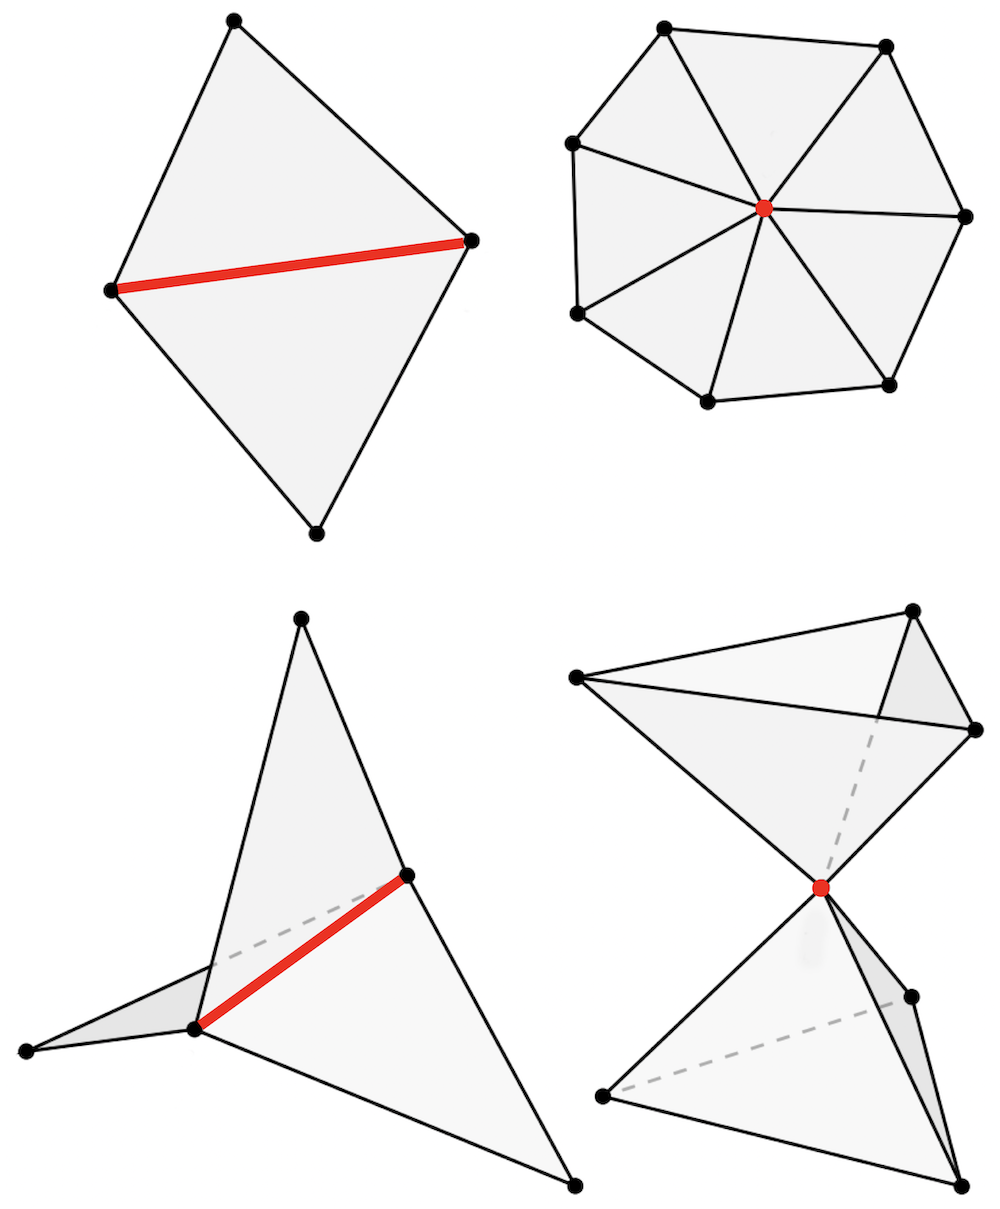
\includegraphics[width=0.9\linewidth]{figures/mesh.png}\\
%
流形边和节点（上）与非流形边和节点（下）的示例。
对于带边界流形，还要定义只属于一个三角形的{\em 边界边}。}
%
%We will denote meshes by $\mathcal{T} = (\mathcal{V},\mathcal{E}, \mathcal{F})$, where $\mathcal{F} =  \{ (i,j,k) : i,j,k \in \mathcal{V} \,\,\, \text{and} \,\,\, (i,j), (i,k), (k,j) \in  \mathcal{E}\}$ and use them as our domain $\Omega$.  


还要进一步假定，每条边恰好由两个三角形共享，并且与每个节点关联的所有三角形之边界构成单一的边环。这一条件保证每个节点周围的一跳邻域都呈圆盘状，从而使网格曲面构成{\em 离散流形}——这样的网格曲面称为{\em 流形网格曲面}。
%In particular, 
%
%
%
与 Riemann 流形类似，可以在网格曲面上定义{\em 度量}。在最简单的情形下，它可以由网格节点 $\mathbf{x}_1, \hdots, \mathbf{x}_n$ 的嵌入诱导，并通过边的 Euclidean 长度 $\ell_{uv} = \| \mathbf{x}_u - \mathbf{x}_v \|$ 表示。
%
按这种方式定义的度量自动满足{\em 三角不等式}等性质，即形如
$
\ell_{uv} \leq \ell_{uq} + \ell_{vq}
$
的表达式对任意 $(u,v,q) \in \mathcal{F}$ 以及任意边的组合都成立。%
%
任何仅用 $\ell$ 即可表达的性质都是{\em 内蕴的}，而任何保持 $\ell$ 的网格曲面形变都是{\em 等距变换}——读者已经从第~\ref{sec:manifolds} 节的讨论中熟悉这些概念。
%


%
%\paragraph{Mesh isometries and rigidity}
%Whether meshes have {\em non-trivial isometries} (i.e. embeddings that do not differ by only a rigid motion) is a deep question with fascinating history. %, and results here are starkly different from the continuous case. 
%%
%In 1766, Leonhard Euler conjectured that every polyhedron (a surface made of polygonal faces, on which a triangular mesh is a particular case) is {\em rigid}: that is, if one imagines a polyhedron as made of metal plates connected by hinges, it would not be possible to move them without bending. This assertion became known as the {\em Rigidity Conjecture} and gave birth to entire theory with the same name.  
%%
%\marginnote{
%\includegraphics[width=1\linewidth]{figures/connelly.png}\\
%%
%A convex polyhedron (icosahedron, left) is rigid by virtue of Cauchy's theorem. A non-convex polyhedron constructed by Klaus Steffen (right) is non-rigid and can be continuously deformed. 
%}
%%
%In 1813, Cauchy succeeded proving that every {\em convex} polyhedron is rigid in 3D \citep{cauchy1813recherche}. 
%%
%In 1897, a Belgian engineer and mathematician Raoul Bricard showed a construction of several flexible polyhedra \citep{bricard1897memoire}, which however, had self-intersections and thus could not be folded out of paper. 
%%
%In 1977, Robert Connelly showed  a non-rigid polyhedron without self-intersections (henceforth called the `Connelly Sphere') finally disproving Euler's conjecture by counter-example \citep{connelly1977counterexample}.  
%%
%A simpler (and in fact the simplest currently known) construction was shown a year later by the German geometry Klaus Steffen; his polyhedron can be easily folded of paper and bent {\em ad libitum}, as shown on the right. Admittedly, this is a very pleasant manual experience,  which the French {\em Institut des Hautes {\'E}tudes Scientifiques} in Bures-sur-Yvette wanted to share with the visitors, installing a metal model of a flexible polyhedron in its library. 
%\joan{This paragraph is very interesting, but it is unclear how it relates to the flow of the section. }

 





\paragraph{Laplacian 矩阵}
%
类比于对图的处理，设有一个包含 $n$ 个节点的（流形）网格曲面，每个节点都关联一个 $d$ 维特征向量；在假定任意一种排序后，可将这些向量排列为一个 $n\times d$ 矩阵 $\mathbf{X}$。
%
这些特征既可以表示节点的几何坐标，也可以表示颜色、法向量等附加属性；在化学等以几何图建模分子的具体应用中，还可以表示原子序数等属性。


先来看
%construction of spectral filters following the 
网格曲面上的谱卷积~（\ref{eqn:conv_spectral}）；需要提醒读者，它源于 Laplacian 算子。
%
把网格曲面视为某个底层连续曲面的离散化，可以将 Laplacian 离散化为
%
\begin{equation}
(\boldsymbol{\Delta}\mathbf{X})_u = \sum_{v \in \mathcal{N}_u} w_{uv} (\mathbf{x}_u - \mathbf{x}_v),  
\label{eq:mesh_lap}
\end{equation}
%
或者用矩阵--向量记号写成 $n\times n$ 对称矩阵 $\boldsymbol{\Delta} = \mathbf{D} - \mathbf{W}$，其中 $\mathbf{D} = \mathrm{diag}(d_1, \hdots, d_n)$ 称为{\em 度矩阵}，$d_u = \sum_{v}w_{uv}$ 称为节点 $u$ 的{\em 度}。
%
不难看出，式~（\ref{eq:mesh_lap}）对邻居特征执行局部的置换不变聚合\linebreak[4] $\phi(\mathbf{x}_u,\mathbf{X}_{\mathcal{N}_u}) =  d_u \mathbf{x}_u - \sum_{v \in \mathcal{N}_u} w_{uv} \mathbf{x}_v$，而 $\mathbf{F}(\mathbf{X}) = \boldsymbol{\Delta}\mathbf{X}$ 实际上正是通用蓝图~（\ref{eq:graph_equivariant}）在构造图上的置换等变函数时的一个实例。
%or, in matrix-vector notation as $\boldsymbol{\Delta} = %\mathbf{D}^{-1}\mathbf{W}$. 


请注意，目前为止式~（\ref{eq:mesh_lap}）中的 Laplacian 定义并没有任何{\em 网格曲面特有}的内容；事实上，这一构造同样适用于任意图，只需将边权重与邻接矩阵对应起来，即 $\mathbf{W} = \mathbf{A}$，也就是 $w_{uv} = 1$\marginnote{此时，度等于邻居的数量。}（当 $(u,v) \in \mathcal{E}$ 时），否则为零。
%
按这种方式构造的 Laplacian 常称为{\em 组合 Laplacian}，以表明它们仅捕获图的连通结构。\marginnote{如果图是有向的，则相应的 Laplacian 是非对称的。}
%
对于几何图（它不一定具有网格曲面的附加结构，但其节点确实具有空间坐标，因而以边长的形式诱导出度量），通常采用与该度量成反比的权重，例如 $w_{uv} \propto e^{-\ell_{uv}}$。



在网格曲面上，可以利用面所提供的附加结构，并用{\em 余切公式} \citep{pinkall1993computing,meyer2003discrete} 定义式~（\ref{eq:mesh_lap}）中的边权重\marginnote{
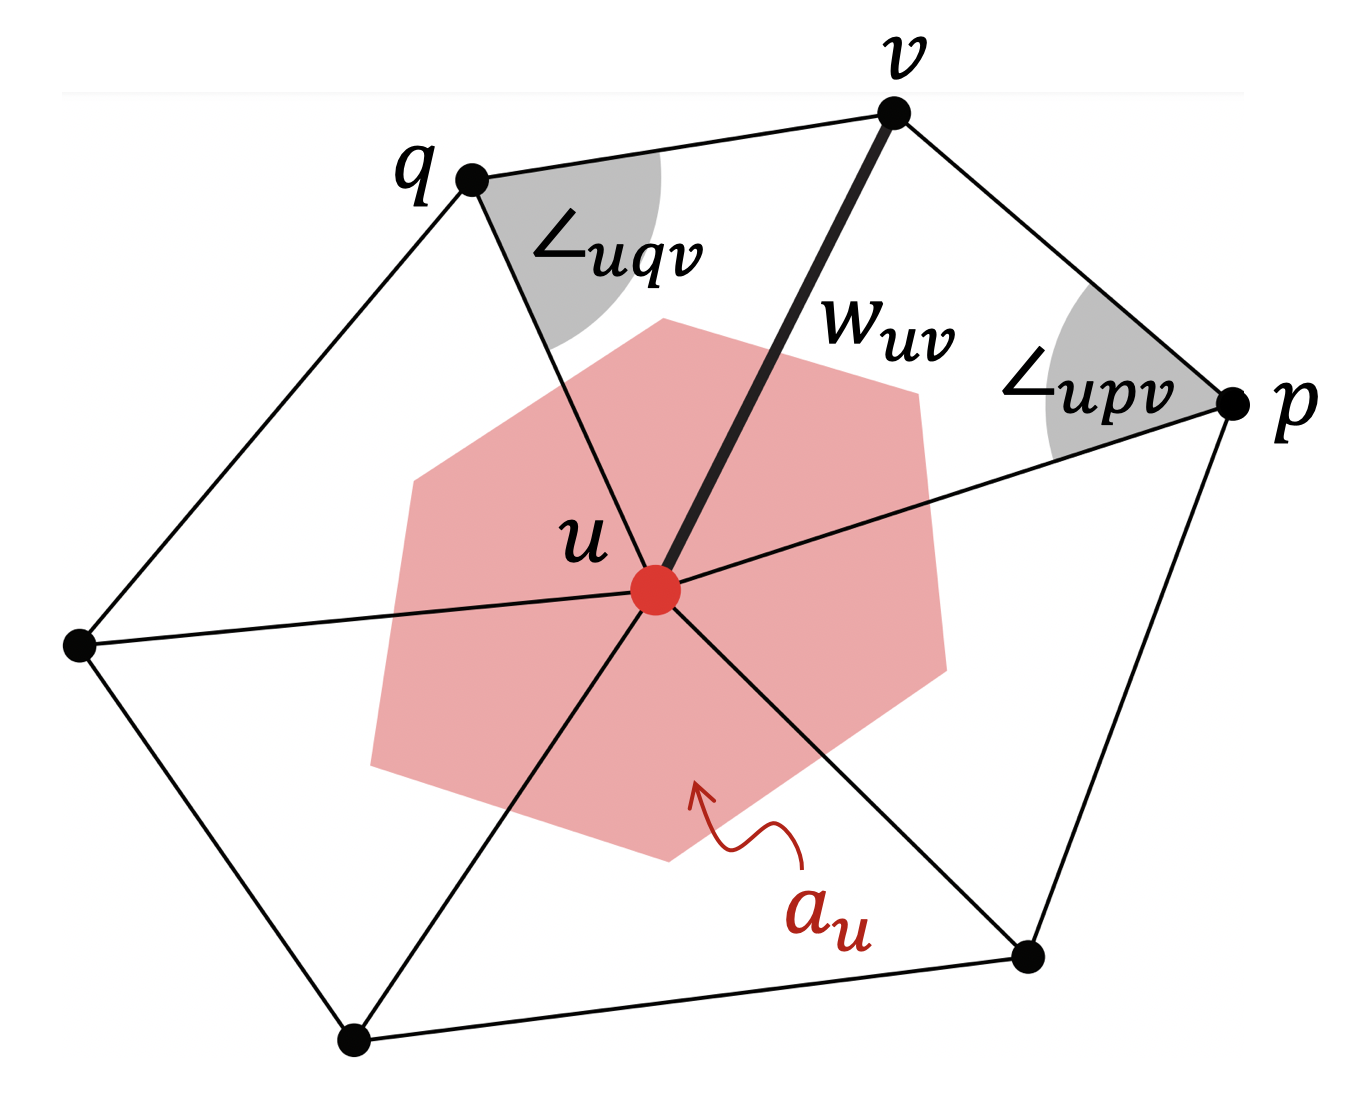
\includegraphics[width=\linewidth]{figures/cotan.png}
这一公式最早见于 \cite{macneal1949solution} 的博士论文；他提出该公式是为了在 Caltech Electric Analog Computer 上求解 PDE。}
\begin{equation}
w_{uv} = \frac{\cot \angle_{uqv} + \cot \angle_{upv}}{2 a_u}
\label{eq:cotan}
\end{equation}
其中，$\angle_{uqv}$ 和 $\angle_{upv}$ 分别是三角形 $(u,q,v)$ 与 $(u,p,v)$ 中共享边 $(u,v)$ 所对的两个角；$a_u$ 是局部面积元，通常计算为由三角形 $(u,p,q)$（它们共享节点 $u$）的重心所构成多边形的面积，即
%
$a_u = \frac{1}{3}\sum_{v,q : (u,v,q) \in \mathcal{F}} a_{uvq}$.


可以证明，余切 Laplacian 具有多种便利性质（例如见 \cite{wardetzky2007discrete}）：它是{\em 半正定}矩阵，$\boldsymbol{\Delta} \succcurlyeq 0$，因而具有可视作频率类比的非负特征值 $\lambda_1 \leq \hdots \leq \lambda_n$；它是对称的，因而具有正交特征向量；并且它是{\em 局部的}（即 $(\boldsymbol{\Delta}\mathbf{X})_u$ 的值只依赖一跳邻居 $\mathcal{N}_u$）。
%
也许最重要的性质是：当网格曲面被无限细化时，余切网格 Laplacian 矩阵 $\boldsymbol{\Delta}$ 收敛于连续算子 $\Delta$ \citep{wardetzky2008convergence}。因此，式~（\ref{eq:cotan}）构成了第~\ref{sec:manifolds} 节所定义 Riemann 流形上 Laplacian 算子的一种恰当{\em 离散化}\marginnote{必须对细化施加一些技术条件，以避免三角形变得病态等情况。一个例子是圆柱面的一种奇异三角剖分，在德文中称为 {\em Schwarzscher Stiefel}（Schwarz's boot），在英文文献中称为 ``Schwarz lantern''；它由因 Cauchy--Schwarz 不等式而闻名的德国数学家 Hermann Schwarz 于 1880 年提出。}。


尽管人们预期 Laplacian 是内蕴的，但这一点从式~（\ref{eq:cotan}）看并不明显；需要经过一些推导，才能将余切权重完全用离散度量 $\ell$ 表示为
$$
w_{uv} = \frac{-\ell^2_{uv} + \ell^2_{vq} + \ell^2_{uq} }{8 a_{uvq}} + 
\frac{-\ell^2_{uv} + \ell^2_{vp} + \ell^2_{up} }{8 a_{uvp}}
$$
%
其中，三角形面积 $a_{ijk}$ 为
$$
a_{uvq} = \sqrt{s_{uvq} (s_{uvq} - \ell_{uv}) (s_{uvq} - \ell_{vq}) (s_{uvq} - \ell_{uq}) }
$$
这里采用{\em Heron 半周长公式}，其中
%$s_{ijk} = \frac{1}{2}(\ell_{ij} + \ell_{ik} + \ell_{jk})$. 
$s_{uvq} = \frac{1}{2}(\ell_{uv} + \ell_{uq} + \ell_{vq})$. 
%
%
这使 Laplacian（以及与之相关的任何量，如其特征向量和特征值）具有{\em 等距不变性}；正因如此，它在几何处理和计算机图形学中备受青睐（见 \cite{wang2019intrinsic} 的优秀综述）：任何不影响度量 $\ell$ 的网格曲面形变（即不“拉伸”或“压缩”网格边）都不会改变 Laplacian。



最后，正如我们已经注意到的，\marginnote{
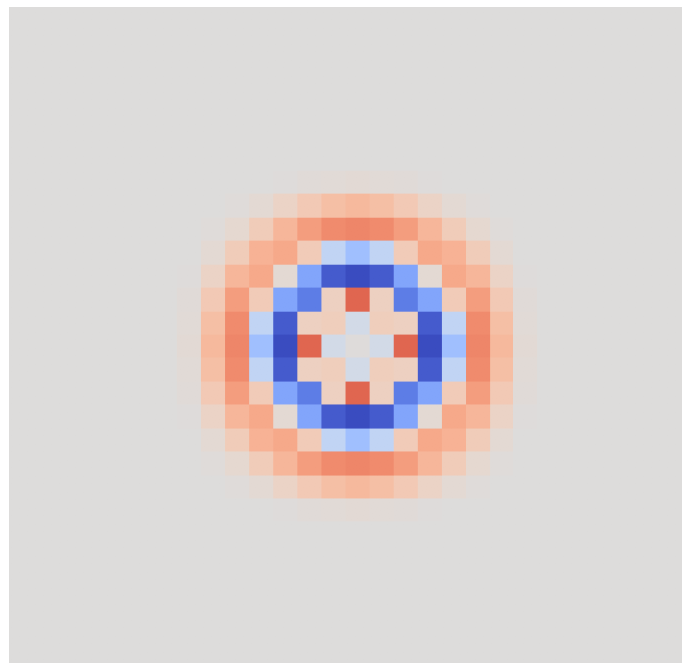
\includegraphics[width=0.9\linewidth]{figures/isotropic.png}
基于 Laplacian 的滤波器是各向同性的。在平面上，这类滤波器具有径向对称性。
} Laplacian 的定义~（\ref{eq:cotan}）对于 $\mathcal{N}_u$ 中节点的置换保持不变，因为它采用了求和形式的聚合。
%
在一般图上，由于邻居缺少规范排序，这是一种不得不接受的限制；而在网格曲面上，可以按照某种定向（例如顺时针）排列一跳邻居，唯一的歧义在于第一个节点的选择。因此，我们无须考虑任意可能的置换，而只需考虑{\em 循环移位}（旋转）；直观地说，这对应于第~\ref{sec:gauges} 节讨论的 $\mathrm{SO}(2)$ 规范变换所产生的歧义。
%
对于固定规范，可以定义对局部方向敏感的{\em 各向异性 Laplacian}；这等价于改变度量或权重 $w_{uv}$。
%
\cite{andreux2014anisotropic,boscaini2016anisotropic} 曾用此类构造设计形状描述符，\cite{boscaini2016learning} 也将其用于早期的网格曲面几何深度学习架构。



\paragraph{网格曲面上的谱分析}
%
将 Laplacian 矩阵对角化的正交特征向量\linebreak[4] $\boldsymbol{\Phi} = (\boldsymbol{\varphi}_1, \hdots, \boldsymbol{\varphi}_n)$（$\boldsymbol{\Delta} = \boldsymbol{\Phi} \boldsymbol{\Lambda} \boldsymbol{\Phi}^\top$，其中 $\boldsymbol{\Lambda} = \mathrm{diag}(\lambda_1, \hdots, \lambda_n)$ 是 Laplacian 特征值的对角矩阵）可用作 Fourier 基的非 Euclidean 类比，从而能把相应 Fourier 变换的乘积作为网格曲面上的谱卷积：
$$
\mathbf{X} \star \boldsymbol{\theta} = 
\boldsymbol{\Phi} \, \mathrm{diag}(\boldsymbol{\Phi}^\top \boldsymbol{\theta}) (\boldsymbol{\Phi}^\top \mathbf{X}) 
=
\boldsymbol{\Phi}\, \mathrm{diag}(\hat{\boldsymbol{\theta}}) \hat{\mathbf{X}},
$$
%
其中，滤波器 $\hat{\boldsymbol{\theta}}$ 直接在 Fourier 域中设计。
%
同样，这个公式中没有任何网格曲面特有的内容，也可以使用一般（无向）图的 Laplacian 矩阵。\marginnote{图为无向图这一假设很重要：此时 Laplacian 是对称的，并具有正交特征向量。}
%
%
利用卷积的这一谱定义把 CNN 推广到图上是一个很自然的想法；事实上，本文的一位作者已在 \cite{bruna2013spectral} 中这样做过。
%
然而，非 Euclidean Fourier 变换似乎
对底层网格曲面或图的微小扰动也极为敏感（见第~\ref{sec:manifolds} 节的图~\ref{fig:mesh_horses}），因此它只能用于处理{\em 固定}域上的不同信号，而不能用于在{\em 不同域}之间泛化。
%
遗憾的是，许多计算机图形学与视觉问题都属于后一类：神经网络在一组 3D 形状（网格曲面）上训练，却在另一组形状上测试，因而基于 Fourier 变换的方法并不适用。

%is given a training set of 3D shapes (meshes) and a different test, the generalisation across domains 



正如第~\ref{sec:manifolds} 节所指出的，更可取的做法是使用形如~（\ref{eqn:conv_spec}）的谱滤波器，即把某个传递函数 $\hat{p}(\lambda)$ 应用于 Laplacian 矩阵：
$$
\hat{p}(\boldsymbol{\Delta})\mathbf{X} = \boldsymbol{\Phi} \hat{p}(\boldsymbol{\Lambda})\boldsymbol{\Phi}^\top\mathbf{X} 
= \boldsymbol{\Phi}\, \mathrm{diag}(\hat{p}(\lambda_1), \hdots, \hat{p}(\lambda_n)) \hat{\mathbf{X}}. 
$$
%
%which can be parametrised with a small number of parameters and computer efficiently. 
%
当 $\hat{p}$ 可以用矩阵--向量乘积表示时，就可以完全避免对 $n\times n$ 矩阵 $\boldsymbol{\Delta}$ 进行特征分解。\marginnote{一般情况下，特征分解的复杂度为 $\mathcal{O}(n^3)$。}
%
例如，\cite{defferrard2016convolutional} 使用 $r$ 次{\em 多项式}作为滤波函数，%in which case the filter is expressed as
$$
\hat{p}(\boldsymbol{\Delta})\mathbf{X} = \sum_{k=0}^r \alpha_k \boldsymbol{\Delta}^k \mathbf{X}  = \alpha_0 \mathbf{X} + \alpha_1 \boldsymbol{\Delta} \mathbf{X}  + \hdots + \alpha_r \boldsymbol{\Delta}^r \mathbf{X}, 
$$
这相当于把 $n\times d$ 特征矩阵 $\mathbf{X}$ 与 $n\times n$ Laplacian 矩阵相乘 $r$ 次。由于 Laplacian 通常是稀疏的（具有 $\mathcal{O}(|\mathcal{E}|)$ 个非零元素），\marginnote{网格曲面是近正则图，每个节点具有 $\mathcal{O}(1)$ 个邻居，因此有 $\mathcal{O}(n)$ 个非零元素位于 $\boldsymbol{\Delta}$ 中。}
%
该运算具有较低的复杂度 $\mathcal{O}(|\mathcal{E}|dr)\sim \mathcal{O}(|\mathcal{E}|)$。
%
此外，由于 Laplacian 是局部的，%(i.e., the value of $(\boldsymbol{\Delta}\mathbf{X})_i$ depends only on 1-hop neighbours, $\mathcal{N}_i$),
$r$ 次多项式滤波器局部化在 $r$ 跳邻域内。


然而，在处理网格曲面时，这一精确性质会带来不利之处，因为滤波器的实际支撑（即其覆盖半径）取决于网格曲面的{\em 分辨率}。
%
必须牢记，网格曲面来自某个底层连续曲面的离散化，因此两个不同网格曲面 $\mathcal{T}$ 和 $\mathcal{T}'$ 可能表示{\em 同一个对象}。\marginnote{    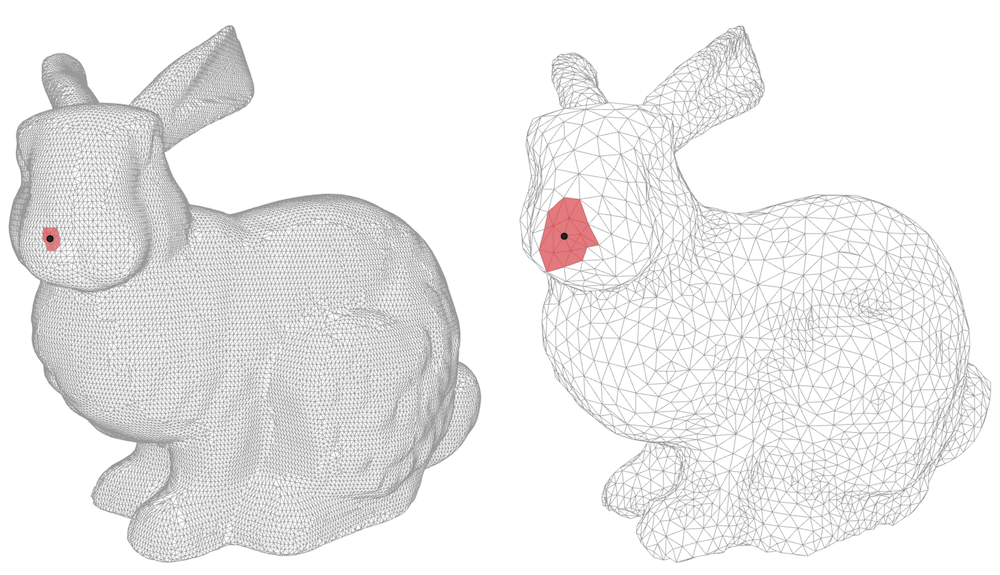
\includegraphics[width=\linewidth]{figures/mesh_res.png}\\
不同分辨率网格曲面上的两跳邻域。}
%
在较细网格曲面上，可能必须使用比粗网格曲面更大的邻域（因而滤波器的次数 $r$ 也更高）。
%

因此，计算机图形学应用中更常使用{\em 有理滤波器}，因为它们与分辨率无关。这类滤波器有多种定义方式（例如见 \cite{patane2020fourier}），最常见的是取某个有理函数（例如 $\frac{\lambda-1}{\lambda+1}$）的多项式。
%
更一般地，可以使用复函数，例如把实直线映射到复平面单位圆上的{\em Cayley 变换} $\frac{\lambda - \mi}{ \lambda + \mi}$。\marginnote{Cayley 变换是 {\em M{\"o}bius 变换}的一种特殊情形。将其作用于 Laplacian（一个半正定矩阵）时，它会把非负特征值映射到复半圆上。}
%
\cite{levie2018cayleynets} 使用表示为{\em Cayley 多项式}的谱滤波器，即具有复系数 $\alpha_l \in \mathbb{C}$ 的实值有理函数：
$$
\hat{p}(\lambda) = \mathrm{Re} \left(  \sum_{l=0}^r 
\alpha_l \left( \frac{\lambda - \mi}{ \lambda + \mi}
\right)^{l}
\right).
$$
%
将 Cayley 多项式应用于矩阵时，其计算需要矩阵求逆：
$$
\hat{p}(\boldsymbol{\Delta}) = \mathrm{Re} \left(  \sum_{l=0}^r
\alpha_l (\boldsymbol{\Delta} - \mi\mathbf{I})^{l} (\boldsymbol{\Delta} + \mi\mathbf{I})^{-l}
\right),\marginnote{In signal processing, polynomial filters are termed {\em finite impulse response} (FIR), whereas rational filters are {\em infinite impulse response} (IIR).}
$$
这一计算可以用线性复杂度近似完成。
%
与多项式滤波器不同，有理滤波器不具有局部支撑，但会指数衰减，%and thus localised
\citep{levie2018cayleynets}.  
%
与直接计算 Fourier 变换相比，一个关键区别在于，多项式滤波器和有理滤波器在底层图或网格曲面的近似等距形变下是稳定的——例如，\cite{levie2018cayleynets,levie2019transferability,gama2020stability,kenlay2021interpretable} 给出了多种此类结果。



%\paragraph{Anisotropic Laplacians}






\paragraph{作为算子的网格曲面与函数映射}


函数映射范式启发我们把网格曲面视为{\em 算子}。如下文所示，这使我们能够利用网格曲面的附加结构，得到更丰富的不变性类型。
%
为便于讨论，假定网格曲面 $\mathcal{T}$ 由坐标为 $\mathbf{X}$ 的嵌入节点构成。
%
如果构造 Laplacian 这样的内蕴算子，可以证明它完整编码了网格曲面的结构，并且能够恢复该网格曲面（精确到其等距嵌入，见 \cite{zeng2012discrete}）。
%
某些其他算子也具有这一性质（例如见 \cite{boscaini2015shape,corman2017functional,chern2018shape}），因此我们将用一般算子，即 $n\times n$ 矩阵 $\mathbf{Q}(\mathcal{T}, \mathbf{X})$，表示网格曲面。


从这一视角看，第~\ref{sec:proto-graphs} 节关于学习形如 $f(\mathbf{X},\mathcal{T})$ 的函数的讨论，%(as we had in our discussion on graphs in Section~\ref{sec:proto-graphs})
可以重新表述为
学习形如 $f(\mathbf{Q})$ 的函数。
%
与图和集合类似，网格曲面的节点同样没有规范排序；也就是说，网格曲面上的函数必须满足置换不变或置换等变条件：
\begin{eqnarray*}
f(\mathbf{Q}) &=& f(\mathbf{P}\mathbf{Q}\mathbf{P}^\top) \\
%
\mathbf{P}\mathbf{F}(\mathbf{Q}) &=& \mathbf{F}(\mathbf{P}\mathbf{Q}\mathbf{P}^\top)
\end{eqnarray*}
% 
上述关系对任意置换矩阵 $\mathbf{P}$ 都成立。
%Conceptually, the permutation matrix can be considered as {\em correspondence} between two isomorphic meshes, i.e., meshes with the same number of nodes and identical connectivity. 
%
%
不过，与一般图相比，这里具有更多结构：可以假定网格曲面来自某个底层连续曲面 $\Omega$ 的离散化。因此，另一个网格曲面 $\mathcal{T}'=(\mathcal{V}',\mathcal{E}',\mathcal{F}')$ 可以由 $n'$ 个节点及其坐标 $\mathbf{X}'$ 构成；它所表示的对象 $\Omega$ 与 $\mathcal{T}$ 所表示的相同。
%\marginnote{It is convenient to think of $\mathcal{T}'$ as a {\em remeshing} of $\mathcal{T}$.}  
%
%
重要的是，网格曲面 $\mathcal{T}$ 和 $\mathcal{T}'$ 可以具有不同的连通结构，甚至具有不同的节点数（$n'\neq n$）。因此，不能把这些网格曲面视为仅仅重新排列了节点的同构图，也不能把置换矩阵 $\mathbf{P}$ 视为二者之间的对应关系。


\cite{ovsjanikov2012functional} 引入了函数映射，把对应关系的概念推广到这类情形：它用{\em 函数}之间的对应关系，取代两个域上{\em 点}之间的对应关系（映射 $\eta : \Omega \rightarrow \Omega'$）；前者由映射 $\mathbf{C}:\mathcal{X}(\Omega) \rightarrow \mathcal{X}(\Omega')$ 给出，见图~\ref{fig:func_maps}。
%
{\em 函数映射}是一个线性算子
$\mathbf{C}$，表示为 $n'\times n$ 矩阵，用于在信号 $\mathbf{x}'$
%\in \mathcal{X}(\mathcal{T}')$  
%defined on the nodes of the mesh of $\mathcal{T}'$ 
与 $\mathbf{x}$ % \in \mathcal{X}(\mathcal{T})$ as
各自所在的域之间建立如下对应关系：
%defined on the nodes of the mesh of $\mathcal{T}$ as 
$$
\mathbf{x}' = \mathbf{C}\mathbf{x}.\marginnote{
In most cases the functional map is implemented in the spectral domain, as a $k\times k$ map $\hat{\mathbf{C}}$ between the Fourier coefficients,
$
\mathbf{x}' = \boldsymbol{\Phi}'\hat{\mathbf{C}}\boldsymbol{\Phi}^\top\mathbf{x},
$
where $\boldsymbol{\Phi}$ and $\boldsymbol{\Phi}'$ are the respective $n\times k$ and $n'\times k$ matrices of the (truncated) Laplacian eigenbases, with $k\ll n,n'$. 
}
$$
%
%
%\michael{[TODO: Typically, $C$ is constructed in the Fourier domain - explain how. We want to have $C$ square to avoid problems with dimensions]}
\cite{rustamov2013map} 证明，为保证映射{\em 保面积}，函数映射必须正交，即 $\mathbf{C}^\top \mathbf{C} = \mathbf{I}$；换言之，它必须是正交群的一个元素 $\mathbf{C} \in \mathrm{O}(n)$。此时，可以用 $\mathbf{C}^{-1} = \mathbf{C}^\top$ 对该映射求逆。


\begin{figure}[h!]
    \centering
    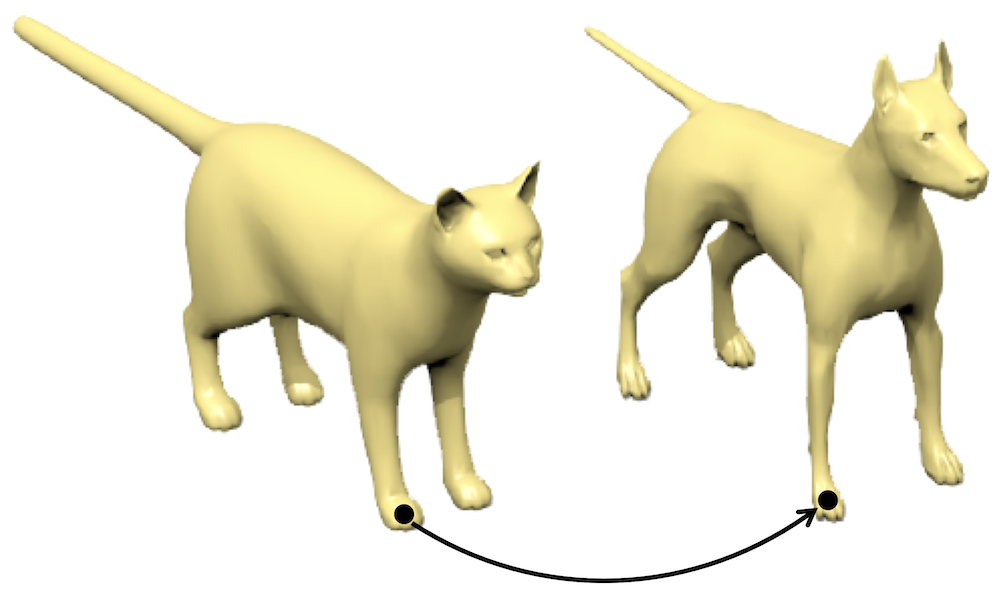
\includegraphics[width=0.45\linewidth]{figures/map_point.png}\hspace{5mm}    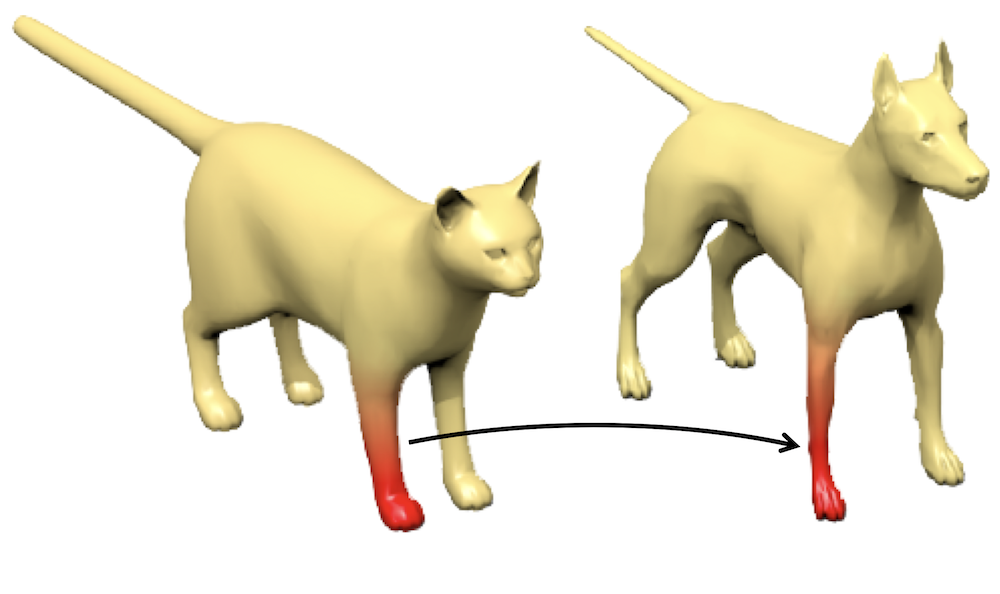
\includegraphics[width=0.45\linewidth]{figures/map_func.png}
    \caption{逐点映射（左）与函数映射（右）。
    }
    \label{fig:func_maps}
\end{figure}%


函数映射还在网格曲面的算子表示之间建立了如下关系：
$$
\mathbf{Q}' = \mathbf{C} \mathbf{Q} \mathbf{C}^\top, \quad \quad \mathbf{Q} = \mathbf{C}^\top \mathbf{Q}' \mathbf{C}, 
$$
%
可以作如下解释：给定算子表示 $\mathbf{Q}$（对应于 $\mathcal{T}$）和函数映射 $\mathbf{C}$，可以构造表示 $\mathbf{Q}'$（对应于 $\mathcal{T}'$）；具体而言，先把信号从 $\mathcal{T}'$ 映射到 $\mathcal{T}$（使用 $\mathbf{C}^\top$），再应用算子 $\mathbf{Q}$，最后映射回 $\mathcal{T}'$（使用 $\mathbf{C}$）。\marginnote{请注意，这些运算按\emph{从右到左}的顺序读取。}
%, i.e. we assume left-multiplication with a signal on $\mathcal{T}'$.}. 
%
由此得到一类更一般的网格曲面上的{\em 重网格化不变}（或等变）函数，它们满足
%
\begin{eqnarray*}
f(\mathbf{Q}) &=& f(\mathbf{C}\mathbf{Q}\mathbf{C}^\top) = f(\mathbf{Q}')\\
%
\mathbf{C}\mathbf{F}(\mathbf{Q}) &=& \mathbf{F}(\mathbf{C}\mathbf{Q}\mathbf{C}^\top) = \mathbf{F}(\mathbf{Q}')
\end{eqnarray*}
% 
上述关系对任意 $\mathbf{C} \in \mathrm{O}(n)$ 都成立。
%
不难看出，前述置换不变性与置换等变性的设定是一个特殊情形；\marginnote{这源于置换矩阵的正交性，即 $\mathbf{P}^\top \mathbf{P} = \mathbf{I}$。}
它可以看作一种只改变节点顺序的平凡重网格化。


\cite{wang2019learning} 证明，给定算子 $\mathbf{Q} = \mathbf{V}\boldsymbol{\Lambda}\mathbf{V}^\top$ 的特征分解，任意重网格化不变（或等变）函数都可以表示为
%
%
$f(\mathbf{Q}) = f(\boldsymbol{\Lambda})$，以及
%
$\mathbf{F}(\mathbf{Q}) = \mathbf{V} \mathbf{F}(\boldsymbol{\Lambda})$, 
%
换言之，重网格化不变函数{\em 仅涉及} $\mathbf{Q}$ {\em 的谱}。
%
%
实践已经证明，Laplacian 特征值的函数对于曲面离散化和扰动具有鲁棒性；这解释了基于 Laplacian 的谱构造为何在计算机图形学以及图深度学习中广受欢迎 \citep{defferrard2016convolutional,levie2018cayleynets}。
%
%In graph deep learning literature, architectures such as ChebNet \citep{defferrard2016convolutional} and CayleyNet \citep{levie2018cayleynets} explicitly learn functions of Laplacian eigenvalues. 
%
%
由于这一结果适用于一般算子 $\mathbf{Q}$，除了无处不在的 Laplacian 之外，还有多种选择——值得注意的例子包括 Dirac 算子 \citep{liu2017dirac,kostrikov2018surface}、Steklov 算子 \citep{wang2018steklov}，以及可学习的参数化算子 \citep{wang2019learning}。


%\michael{The degree of freedom we have is the operator itself - which leads to learnable operators.}

%\joan{We might want to mention extrinsic models that build anisotropy based on the Dirac Operator rather than the Laplace operator; Crane et al, and our Surface Network paper}
%\joan{This section clearly needs to branch out into its own chapter. }


\section{几何深度学习模型}

在深入研究了几何深度学习蓝图的各种实例化形式（对应于域、对称群和局部性概念的不同选择）之后，我们现在可以讨论如何通过实施这些准则得到若干最流行的深度学习架构。

我们的论述仍不严格按照一般性程度排序。首先介绍三类几乎可以直接根据前文讨论实现的架构：卷积神经网络（CNN）、群等变 CNN 和图神经网络（GNN）。

随后，我们将进一步考察图结构事先未知（即无序集合）时的 GNN 变体，并在讨论中把流行的 Deep Sets 和 Transformer 架构描述为 GNN 的实例。

在关于几何图和网格的讨论之后，我们首先描述等变消息传递网络，它将显式几何对称性引入 GNN 计算。然后，我们说明如何在深度学习中具体实现测地线和规范对称性理论，由此得到一族内蕴网格 CNN（包括 Geodesic CNN、MoNet 和规范等变网格 CNN）。

最后，我们从\emph{时间}角度重新审视网格域。该讨论将引出循环神经网络（RNN）。我们将说明 RNN 在时间网格上如何具有平移等变性，同时还将研究它们对于时间扭曲变换的稳定性。这一性质对于恰当处理长程依赖十分必要，而要求模型类对这类变换具有不变性，恰好得到门控 RNN 这一类别（包括 LSTM 或 GRU 等流行的 RNN 模型）。%Given that we aim to study time warping invariance in greater detail (and not just describe a model class), this subsection will be longer than the others.

我们希望上述内容涵盖了写作本文时正在使用的大多数关键深度学习架构，但也清楚新的神经网络实例每天都在提出。因此，我们并不试图涵盖每一种可能的架构，而是希望以下各节具有足够的示范性，使读者能够从不变性与对称性的视角轻松归类几何深度学习未来的任何发展。

\subsection{卷积神经网络}
\label{sec:cnnsec}

卷积神经网络或许是遵循第~\ref{sec:gdl_blueprint} 节所述几何深度学习蓝图的最早且最著名的深度学习架构实例。
%
%
% ====
%
在第 \ref{sec:grids_euclidean} 节中，我们已经完整刻画了线性、局部的平移等变算子类，它由
卷积 ${\bf C(\thetab)}{\bf x} = {\bf x} \star \thetab$ 给出，其局部化滤波器为 $\thetab$\marginnote{回顾一下，${\bf C}(\boldsymbol{\theta})$ 是以 $\boldsymbol{\theta}$ 为参数的\emph{循环}矩阵。}。
我们首先关注标量值（“单通道”或“灰度”）离散图像，
%${\bf x}$ (having a single channel), 
其中，
域是网格 $\Omega = [H] \times [W]$，且 $\mathbf{u} = (u_1, u_2)$、${\bf x} \in \gX(\Omega, \R)$。

任何采用大小为 $H^f \times W^f$ 的紧支撑滤波器的卷积，
都可以写成生成元 $\thetab_{1,1}, \dots, \thetab_{{H^f,W^f}}$ 的线性组合；例如，这些生成元可由单位峰 $\boldsymbol{\theta}_{vw}(u_1, u_2) = \delta(u_1 - v, u_2 - w)$ 给出。因此，任何局部线性等变映射均可表示为\marginnote{注意，我们通常把 $\vec{x}$ 和 $\boldsymbol{\theta}_{vw}$ 视为二维矩阵，但在此公式中，$\vec{x}$ 和 $\boldsymbol{\theta}_{vw}$ 的两个坐标维度都被\emph{展平}为一个维度，从而使 $\vec{x}$ 成为向量、$\vec{C}(\boldsymbol{\theta}_{vw})$ 成为矩阵。}%directional derivatives $\thetab_{ij}(u_1,u_2) = \delta(u_1, u_2) - \delta(u_1-i,u_2-j), (i,j) \neq (0,0) $ plus the local average $\thetab_{0}(u_1,u_2) = \Delta^{-2}$. % \taco{I guess delta here is a function that equals 1 at (0,0) and 0 elsewhere? Could also mean 1 when u1 = u2, or it could be the Dirac delta which is infinite at zero... Maybe clarify. Also if my first guess is correct, is this really a basis? Can we express the filter which is 1 in the center and 0 elsewhere, i.e. delta(u1, u2)? Finally, just using a basis of delta peaks on each pixel might be more intuitive than directional derivatives?}
%\joan{Yes, here we used directional derivatives as analogy with graphs, in which derivative filters (Adjacency being lowpass filter and Laplacian being high-pass) are intrinsically defined. Correct I missed the average in the family of generators }
\begin{equation}
    \mathbf{F}(\mathbf{x}) = \sum_{v=1}^{H^f}\sum_{w=1}^{W^f} \alpha_{vw} \mathbf{C}(\thetab_{vw})\mathbf{x}~, 
\end{equation}
在坐标表示下，这对应于熟悉的二维卷积（概览见图 \ref{fig:2dconv}）：
\begin{figure}
     \centering
     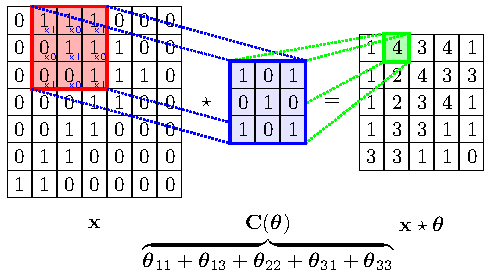
\includegraphics[width=0.7\linewidth]{figures/2d_conv.pdf}
     \caption{图像 $\vec{x}$ 与滤波器 $\vec{C}(\boldsymbol{\theta})$ 进行卷积的过程。滤波器参数 $\boldsymbol{\theta}$ 可以表示为生成元 $\boldsymbol{\theta}_{vw}$ 的线性组合。}
     \label{fig:2dconv}
\end{figure}
\begin{equation}\mathbf{F}(\mathbf{x})_{uv}= \sum_{a=1}^{H^f}\sum_{b=1}^{W^f} {\alpha}_{ab} x_{u+a, v+b}~.
\end{equation}
也可以选择其他基 $\boldsymbol{\theta}_{vw}$，它们将产生等价的运算（但 $\alpha_{vw}$ 的选择可能不同）。一个常见例子是把\emph{方向导数} $\thetab_{vw}(u_1,u_2) = \delta(u_1, u_2) - \delta(u_1-v,u_2-w), (v,w) \neq (0,0) $ 与局部平均 $\thetab_{0}(u_1,u_2) = \frac{1}{H_fW_f}$ 一并使用。事实上，方向导数可以看作图上扩散过程在网格上的对应物：若假设每个像素都是与网格中相邻像素相连的节点，便可恢复这一对应关系。

当标量输入通道替换为多个通道（例如 RGB 颜色通道，或更一般地，任意数量的\emph{特征图}）时，卷积滤波器就成为一个{\em 卷积张量}，表示输入特征到输出特征图的任意线性组合。在坐标表示下，可以写为
%
\begin{equation}
\label{eq:basiccnnlayer}
\mathbf{F}(\mathbf{x})_{uvj}= \sum_{a=1}^{H^f}\sum_{b=1}^{W^f}\sum_{c=1}^M {\alpha}_{jabc} x_{u+a, v+b, c}~,~ j\in[N]~,
\end{equation}
%
其中，$M$ 和 $N$ 分别为输入通道数和输出通道数。
这一基本运算涵盖了一大类神经网络架构；下一节将说明，这些架构对计算机视觉、信号处理及其他许多领域产生了深远影响。这里，我们不去逐一剖析 CNN 数量繁多的可能架构变体，而是着重讨论促使其得到广泛应用的一些关键创新。



\paragraph{高效的多尺度计算}
正如一般对称性的 GDL 模板所讨论的，从卷积算子 $\mathbf{F}$ 中提取平移不变特征需要一个非线性步骤。\marginnote{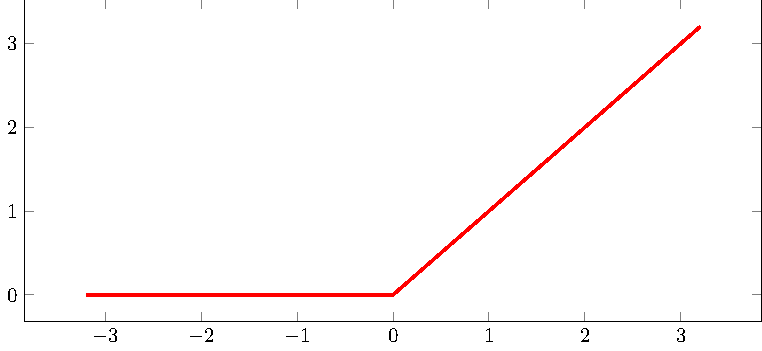
\includegraphics[width=\linewidth]{figures/relu.pdf}\\ ReLU 常被视为一种“现代”架构选择，但早在 Neocognitron 中就已使用 \citep{fukushima1982neocognitron}。整流等价于解调原理；解调是电气工程的基础，支撑了 FM 广播等多种传输协议，在神经元活动模型中也具有重要作用。}%so that the energy captured along each sub-band $\thetab_{ij}$ is mapped towards the low-frequencies
卷积特征通过一个非线性的%rectification stage,
\emph{激活函数} $\sigma$ 处理；该函数逐元素作用于输入，即 $\sigma: \gX(\Omega) \to \gX(\Omega)$，且 $\sigma(\mathbf{x})(u) = \sigma(\mathbf{x}(u))$。写作本文时最流行的例子或许是修正线性单元（ReLU）：$\sigma(x) = \max(x, 0)$。%, or other choices of activation function.
这种非线性会有效地对信号进行\emph{整流}，将其能量推向较低频率，并通过迭代这一构造，使跨尺度的高阶交互计算成为可能。

早在 \cite{fukushima1982neocognitron} 和 \cite{lecun1998gradient} 的早期工作中，CNN 及类似架构
%Since the early days from Fukushima and LeCun, CNN architectures 
就已经采用多尺度结构：在每个卷积层（\ref{eq:basiccnnlayer}）之后执行一次网格粗化
$\mathbf{P} : \gX(\Omega) \to \gX(\Omega')$，其中网格 $\Omega'$ 的分辨率比 $\Omega$ 更粗。
这使多尺度滤波器能够有效增大感受野，同时保持每个尺度上的参数数量恒定。
%
可以采用多种信号粗化%or
策略 $\mathbf{P}$（称为\emph{池化}），其中最常见的是%possible: either %by %explicitly
先应用低通抗混叠滤波器（如局部平均），再对网格下采样，或者采用非线性最大池化。
%
%
%Inspired by neuroscience, 

总之，一个“基础”CNN 层可以表示为几何深度学习蓝图中已经引入的基本对象之复合：
\begin{equation}
    \mathbf{h} = \mathbf{P}(\sigma(\mathbf{F}( \mathbf{x})))~,
\end{equation}
即等变线性层 $\mathbf{F}$、粗化运算 $\mathbf{P}$ 和非线性函数 $\sigma$。还可以在 CNN 中执行平移不变的\emph{全局}池化运算。直观地说，每个像素在若干次卷积后都概括了一个以自身为中心的\emph{斑块}，并据此\emph{提出}图像的最终表示\marginnote{仅由本段所述运算组成的 CNN 常称为“全卷积”网络。相比之下，许多 CNN 在应用足够多的等变层和粗化层后，会沿空间轴\emph{展平}图像并将其传给 MLP 分类器；这样会失去平移不变性。}；最终选择由某种对这些提议的聚合方式决定。平均函数是一种常见选择，因为无论图像大小如何，其输出都能保持相近的量级 \citep{springenberg2014striving}。

图 \ref{fig:cnn_drawn_plot} 展示了遵循这一 CNN 蓝图的若干著名实例，其中一些将在下文讨论。

\begin{figure}
    \centering
    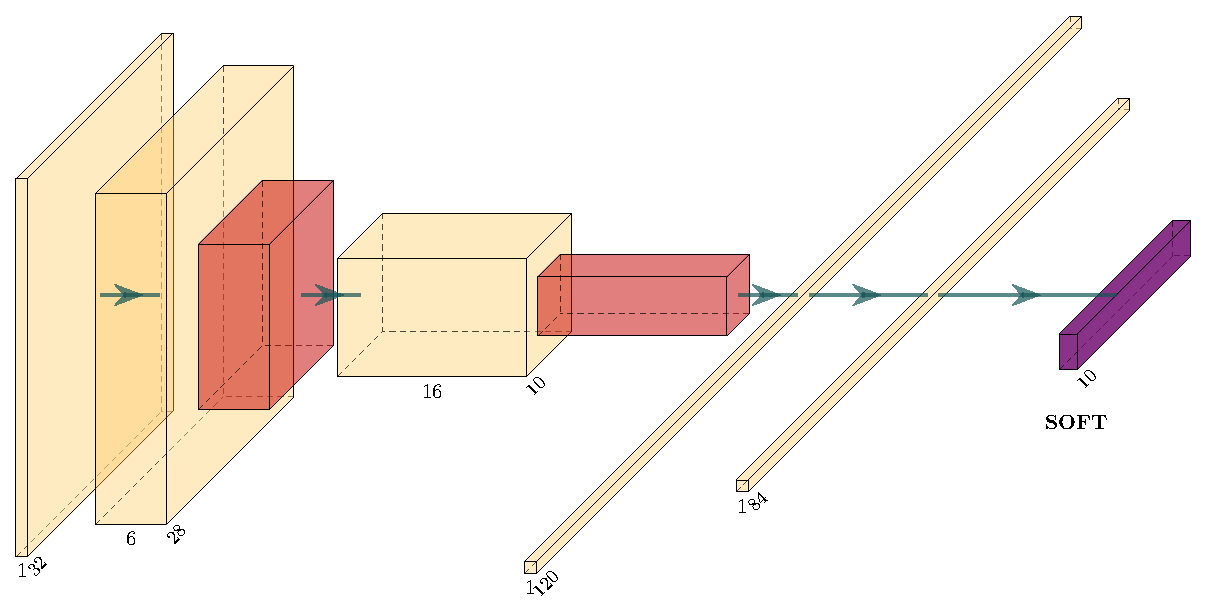
\includegraphics[width=0.85\textwidth]{figures/lenet.pdf}
    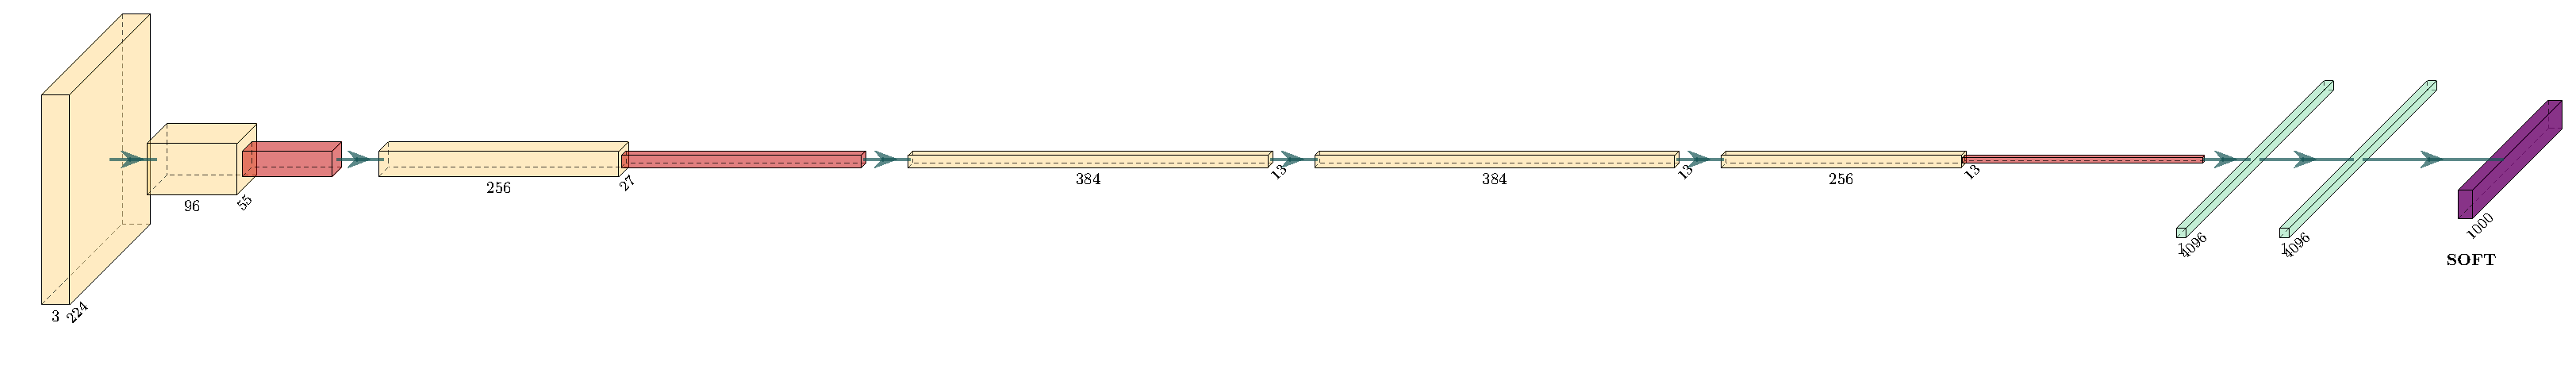
\includegraphics[width=0.85\textwidth]{figures/alexnet.pdf}
    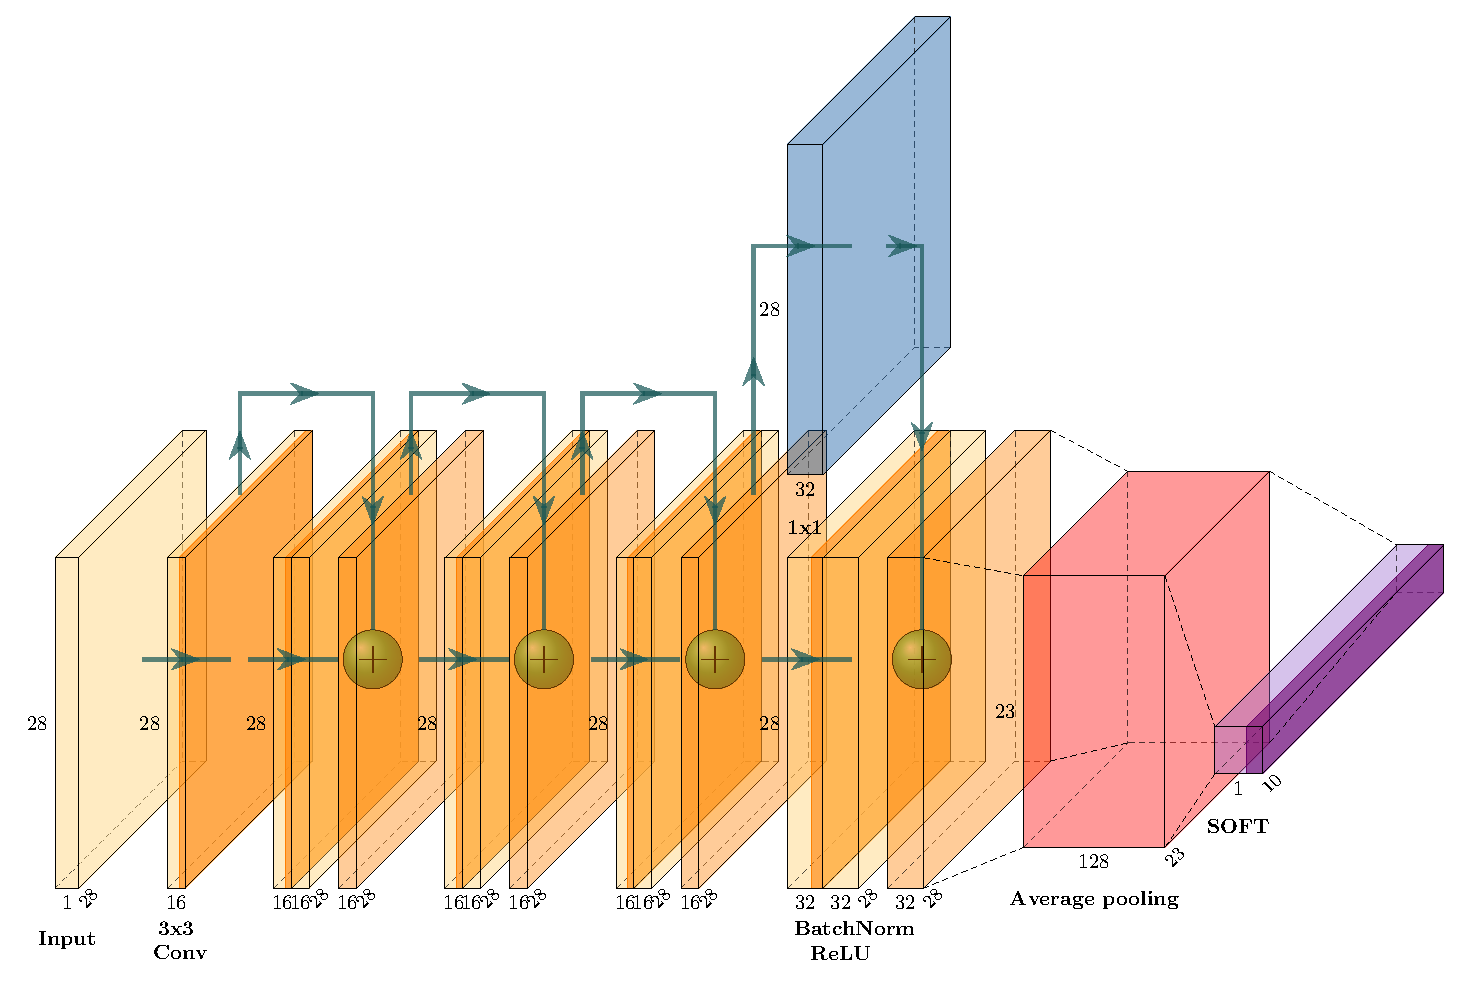
\includegraphics[width=0.85\textwidth]{figures/resnet.pdf}
    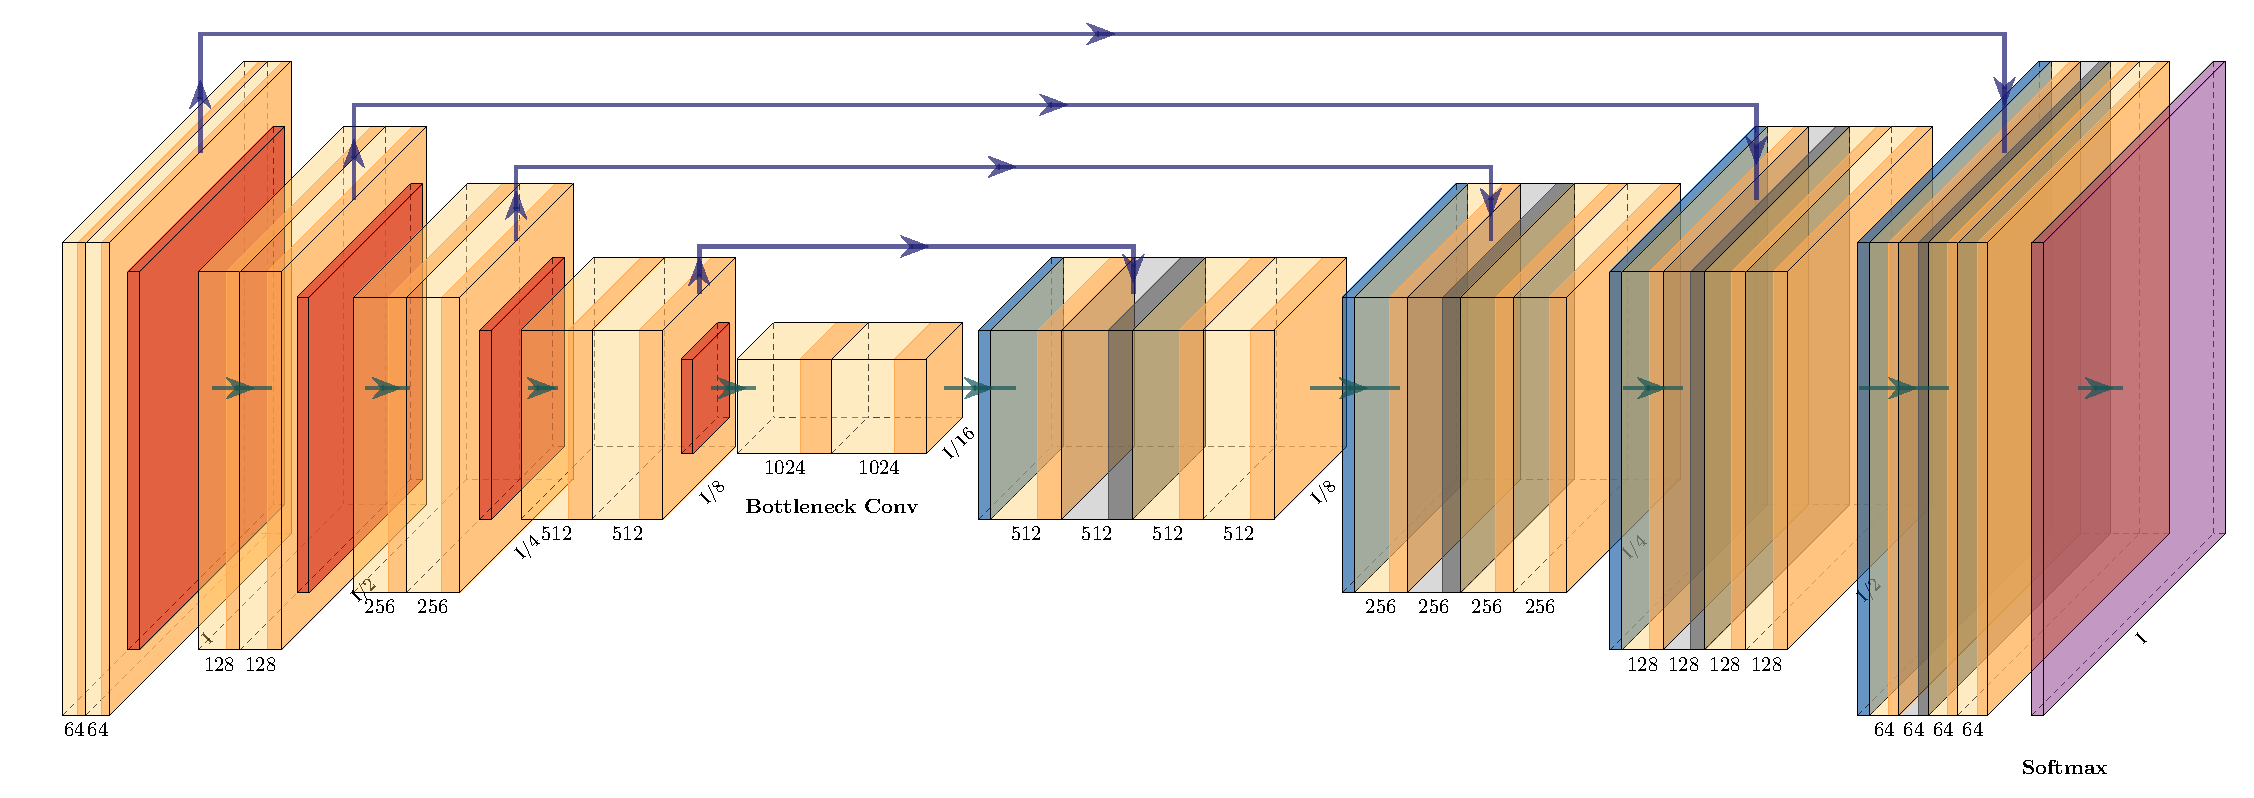
\includegraphics[width=0.85\textwidth]{figures/Unet.pdf}
    \caption{著名的 CNN 架构实例。\textbf{从上到下}：LeNet \citep{lecun1998gradient}、AlexNet \citep{krizhevsky2012imagenet}、ResNet \citep{he2016deep} 和 U-Net \citep{ronneberger2015u}。使用 PlotNeuralNet 包绘制 \citep{haris2018}。}
    \label{fig:cnn_drawn_plot}
\end{figure}
%role of depth
\paragraph{深层网络与残差网络}
因此，在最简单的形式下，CNN 架构由超参数\linebreak[4] $(H^f_k, W^f_k, N_k, p_k )_{k \leq K}$ 指定，其中 $M_{k+1} = N_k$，而 $p_k=0,1$ 表示是否执行网格粗化。虽然这些超参数在实践中都很重要，但一个尤其重要的问题是理解深度 $K$ 在 CNN 架构中的作用，以及选择这一关键超参数所涉及的基本权衡，特别是它与滤波器大小（$H_k^f, W_k^f$）之间的关系。

尽管这一问题尚无严格答案，近年来不断积累的经验证据表明，更深（$K$ 较大）而更窄（$(H^f_k, W^f_k)$ 较小）的模型具有更有利的权衡\marginnote{
从历史上看，ResNet 模型之前已有\emph{高速公路网络} \citep{srivastava2015highway}，后者允许用更一般的\emph{门控}机制控制残差信息流。}。在这一背景下，\cite{he2016deep} 的关键洞见是对每个卷积层重新参数化，使其建模前一层特征的\emph{扰动}，而不是一般的非线性变换：
\begin{equation}
    \mathbf{h} = \mathbf{P}\left(\mathbf{x} + \sigma(\mathbf{F}(\mathbf{x})) \right)~.
\end{equation}
由此得到的\emph{残差}网络相较前一种表述具有若干关键优势。本质上，残差参数化与如下观点一致：深度网络是底层连续动力系统的离散化，而该系统由常微分方程（ODE）建模\marginnote{在这种情况下，ResNet 正在对 ODE 执行前向 Euler 离散化：$\dot{\mathbf{x}} = \sigma( \mathbf{F}(\mathbf{x}))$。}。关键在于，事实证明，通过建模速度来学习动力系统远比直接学习其位置容易。在我们的学习设定中，这意味着优化景观具有更有利的几何形态，因而能够训练比以往深得多的架构。正如未来工作将讨论的那样，使用深度神经网络进行学习定义了一个非凸优化问题；在某些简化情形下，该问题可以用梯度下降方法高效求解。ResNet 参数化的关键优势已经在简单情形中得到严格分析 \citep{hardt2016identity}，并且仍是理论研究的活跃方向。
最后，Neural ODE \citep{chen2018neural} 是近期一种流行架构，它直接学习 ODE $\dot{\mathbf{x}} = \sigma( \mathbf{F}(\mathbf{x}))$ 的参数并依赖标准数值积分，从而进一步推进了与 ODE 的类比。

%\michael{This is also the case for GNNs, which are a discretization of a nonlinear diffusion PDE} \petar{skipping for now, as discussed with Michael}

%Normalization 
\paragraph{归一化}
另一个显著提升 CNN 经验性能的重要算法创新是\emph{归一化}。早期的神经活动模型假设，神经元会执行某种形式的局部“增益控制”，其中层系数 $\mathbf{x}_{k}$ 被替换为 $\mathbf{\tilde{x}}_{k} = \sigma_k^{-1} \odot (\mathbf{x}_{k} - \mu_k)$。这里，$\mu_k$ 和 $\sigma_k$ 分别编码 $\mathbf{x}_k$ 的一阶矩与二阶矩信息；它们既可以全局计算，也可以局部计算。

在深度学习中，这一原理通过\emph{批归一化}层 \citep{ioffe2015batch} 得到广泛采用\marginnote{需要指出的是，在批归一化出现以前，对神经网络激活进行归一化就已经受到关注；例如见 \cite{lyu2008nonlinear}。}，随后又产生了若干变体 \citep{ba2016layer,salimans2016weight,ulyanov2016instance,cooijmans2016recurrent,wu2018group}。
尽管已有工作试图从条件更良好的优化景观角度严格解释归一化的益处 \citep{santurkar2018does}，但在写作本文时，仍然缺少能够提供指导原则的一般理论。

\paragraph{数据增强}
CNN 虽然编码了与平移不变性和尺度分离相关的几何先验，却没有显式考虑其他已知的语义保持变换，例如光照或颜色变化，以及小幅旋转和缩放。以最小架构改动纳入这些先验的一种实用方法是进行\emph{数据增强}，即手动对输入图像施加上述变换，并把所得图像加入训练集。

数据增强在经验上取得了成功并得到广泛应用：它不仅用于训练最先进的视觉架构，还推动了自监督表示学习和因果表示学习的多项发展 \citep{chen2020simple,grill2020bootstrap,mitrovic2020representation}。然而，从样本复杂度看，它已被证明是次优的 \citep{mei2021learning}；更高效的策略是考虑具有更丰富不变群的架构，这正是下文要讨论的内容。

%TODO: discuss Preserving Orientation: contrast this with the GNN setting. 

% ====

% To define a convolutional operator, we will consider the case of 2D inputs (i.e. single-channel images), $\vec{X}\in\mathbb{R}^{h\times w}$. Let $\vec{K}\in\mathbb{R}^{n\times m}$ be a small \emph{kernel matrix} (typically, $n = m = 3$ in modern neural network architectures). The kernel is overlaid in all possible ways
% over the input (see Figure \ref{fig:2dconv}), recording sums of elementwise products to create a
% new image, $\vec{X}'$:\marginnote{It should be noted that this approach is actually cross‐correlation rather than the convolution; but, for purposes of machine learning, the two are equivalent.}
% \begin{equation}
%     x'_{ab} = \sum_{i=1}^n\sum_{j=1}^m k_{ij}x_{a+i-1,b+j-1}
% \end{equation}
% The image is typically padded with sufficiently many zeroes on the edges, to ensure that the size of the output matches the size of the input.

% Moving from here to a convolutional \emph{layer} requires a few extensions. If the input has multiple channels, the kernel matrix is \emph{extended} in the channel dimension to match the input. This \emph{kernel tensor} specifies a single output channel. Each output channel requires a separate kernel tensor. Lastly, a channel‐specific bias and nonlinearity may be applied to obtain the final output image (sometimes known as a \emph{feature map}). 

% In summary, to process an input image $\vec{X} \in \mathbb{R}^{h\times w\times d}$ using a convolutional layer computing $d'$ channels, we require a kernel tensor $\vec{K}\in\mathbb{R}^{n\times m\times d\times d'}$ and a bias vector $\vec{b}\in\mathbb{R}^{d'}$, and proceed as follows:\marginnote{\includegraphics[width=\linewidth]{figures/fullconv.png}}
% \begin{equation}
%     x'_{abc} = \sigma\left(b_c + \sum_{i=1}^n\sum_{j=1}^m\sum_{k=1}^d k_{ijkc}x_{a+i-1,b+j-1,k}\right)
% \end{equation}

% This layer clearly exploits the structure present in an image, with neighbouring pixels
% influencing each other far more strongly than ones on opposite corners. The operator is
% also \emph{translation equivariant}, as required for grids: as the same kernels are applied identically across each image patch, we are encoding a structural bias that a feature of interest is important, no matter where it occurs in the image.

% Often, we are interested in computing outputs on the level of \emph{entire} images. Hence it is useful to compress an image to a \emph{flat} representation, but doing so on the input image sizes often results in an overly large vector (of size $O(hwd)$. Accordingly, once a sufficient number of convolutions has been applied to the input, it is very common to \emph{downsample} the image. 

% As convolutions \emph{``light up''}\marginnote{\includegraphics[width=\linewidth]{figures/maxpool.png}} (return high values) when a certain
% pattern of interest is detected in the input, when summarising the image it makes sense
% to preserve \emph{maximally activated} components of it. This motivates the \emph{max‐pooling} layer, which takes $n\times m$ (usually disjoint, with $n = m = 2$) image patches across each channel and summarises them by taking only the maximal pixel value.

% \michael{This is certainly not the most important reason for using nonlinear pooling - I think we want to refer to Bruna, Mallat 2012 here}

% \begin{figure}
%     \centering
%     \includegraphics[width=\linewidth]{figures/fig_conv.png}
%     \caption{An overview of a typical CNN architecture for image classification. Convolutional and pooling layers are interleaved, with the depth (number of features computed per pixel) increased at the expense of height and width. Once the images are small enough, they are flattened into 1D, and an MLP is used to classify them.}
%     \label{fig:figconv}
% \end{figure}

% Note that a $2\times 2$ max‐pooling layer (which is most common) will preserve only a quarter of the pixels, while leaving the channel axis unchanged. This provides more space
% for gradually increasing the channel size, and therefore computing a richer quantity of
% higher‐level features. A typical convolutional neural network architecture thus consists
% of a series of interleaved convolutional and pooling layers, until the input is reduced sufficiently to be processed by an MLP---as in Figure \ref{fig:figconv}.

% It is also possible, though less common, to perform \emph{global} pooling operations within CNNs. Intuitively, this involves each pixel---which, after several convolutions, summarises a \emph{patch} centered around it---\emph{proposing} the final representation of the image, with the ultimate choice being guided by a form of aggregation of these proposals. A popular choice here is the average function, as its outputs will retain similar magnitudes irrespective of the image size \citep{springenberg2014striving}.

% It is generally perceived that, for image recognition tasks, deep convolutional networks
% strongly draw their outperformance from both their depth \textbf{and} their parameter tying. However, training very deep convolutional networks used to be notoriously difficult. As shown by \citet{he2016deep}, overly deep convolutional networks \emph{do not overfit}, as their training performance degrades along with their testing performance. This is somewhat counterintuitive, as increased depth not only comes with larger parameter spaces to optimise, but moreover, if the additional layers are useless to learning good representations,
% the layer could simply choose to \emph{ignore} them (by learning the \textbf{identity} function).

% Through this counterintuitive property, the authors proposed an obvious fix: the \emph{residual (skip) connection} \citep{he2016deep}, which ``shortcuts'' a particular block of operations in a neural
% network. If a neural network block computes a function $f(\vec{x})$, a skip connection allows $\vec{X}$ to directly reach the output of this block through aggregation; i.e. the neural network simply computes $f(\vec{x}) + \vec{x}$. More generally, if the block changes the input dimensionality, a simple linear projection may be introduced to correct for this:
% \begin{equation}
%     \widetilde{f}(\vec{x}) = f(\vec{x}) + \vec{W}_\mathrm{skip}\vec{x} 
% \end{equation}
% Note that, effectively, this operation allows signals to directly reach deeper stages of the
% input processing, and therefore allows the network to choose its own depth. This turned
% out to be a very powerful and versatile concept, that enabled a 152‐layer network to win
% the ImageNet competition in 2015. Currently, it is ubiquitous in deep learning. It is worth noting that such (``ResNet'') models are predated by \emph{highway networks} \citep{srivastava2015highway}, which allow for more general \emph{gating} mechanisms to control the residual information flow.

% \michael{Scale separation and pooling - show here how pooling makes approximate translation invariance?}





\subsection{群等变 CNN}

正如第 \ref{sec:groups} 节所讨论的，我们可以把卷积运算从欧氏空间上的信号推广到任意\emph{齐性空间} $\Omega$ 上的信号，其中群 $\fG$ 作用于该空间\marginnote{回顾一下，齐性空间是配备传递群作用的集合 $\Omega$；这意味着对于任意 $u,v \in \Omega$，都存在 $\fg \in \fG$ 使得 $\fg. u = v$。}。
在欧氏卷积中，经过{\em 平移的}滤波器会与信号进行匹配；与此类似，群卷积的思想是利用群作用在域上移动滤波器，例如对其进行旋转和平移。
借助群作用的\emph{传递性}，我们可以把滤波器移动到 $\Omega$ 上任意位置。
本节将讨论群卷积这一一般思想的若干具体实例，包括实现细节和架构选择。

%, including discrete roto-translation equivariant planar and 3D CNNs, convolutions on the group of symmetries of a DNA sequence, and spherical CNNs.

\paragraph{离散群卷积}

我们先考虑域 $\Omega$ 和群 $\fG$ 都是离散的情形。
%
第一个例子是表示为三维网格上信号的医学体数据图像%(e.g. medical scans)
，它具有离散平移和旋转对称性。%,
%and DNA sequences with translation symmetry as well as so-called \emph{reverse-complement} symmetry (explained below).
%
%For the first example, we take as 
域是三维立方网格 $\Omega = \Z^3$，而图像（例如
MRI 或 CT 三维扫描）被建模为函数 $x : \Z^3 \rightarrow \R$，即 $x \in \mathcal{X}(\Omega)$。
尽管实践中这类图像的支撑位于有限长方体 $[W] \times [H] \times [D] \subset \Z^3$ 上，我们仍倾向于把它们看作 $\Z^3$ 上经过适当零填充的函数。
%that happen to be zero outside a finite region. 
%
作为对称性，我们考虑群 $\fG = \Z^3 \rtimes O_h$，它由 $\Z^3$ 上保持距离和定向的变换组成。
该群由平移（$\Z^3$）和离散旋转 $O_h$ 组成，后者由绕三个坐标轴的 $90$ 度旋转生成（见图 \ref{fig:cayley-diagram-Oh}）。

\begin{figure}[h!]
    \centering
    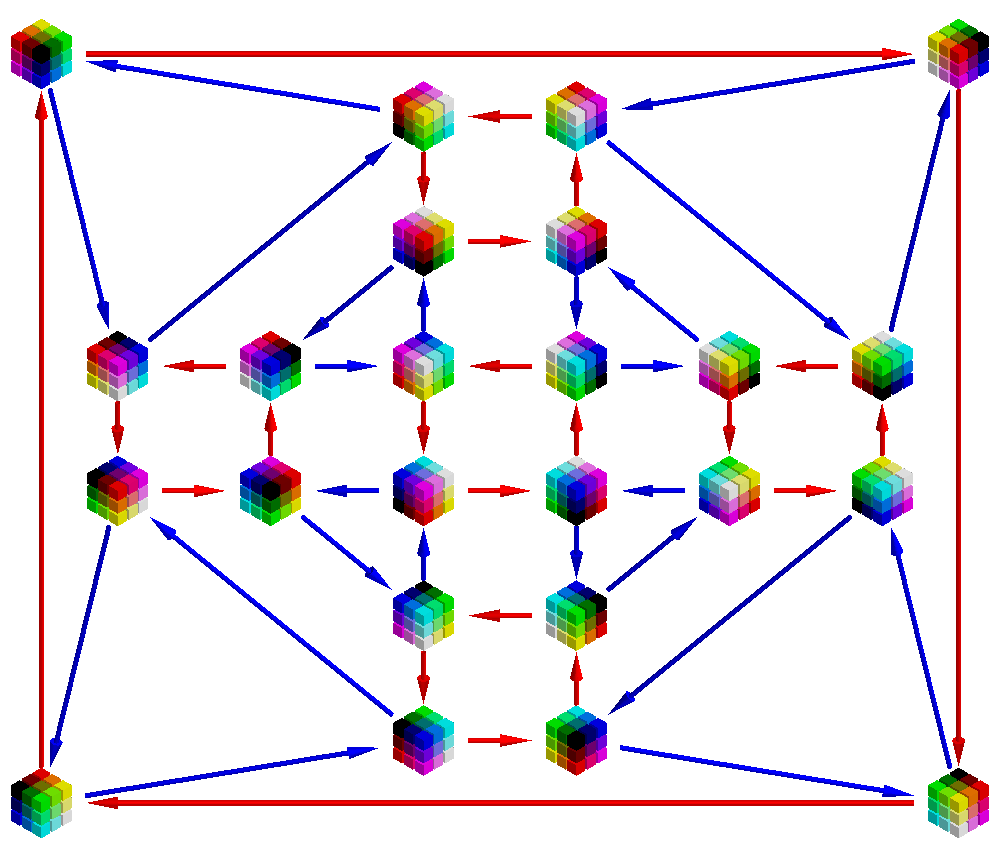
\includegraphics[width=0.6\textwidth]{figures/Oh}
    \caption{一个 $3 \times 3$ 滤波器经全部 $24$ 个离散旋转群元素 $O_h$ 旋转后的结果；该群由绕竖直轴的 $90$ 度旋转（红色箭头）和绕对角轴的 $120$ 度旋转（蓝色箭头）生成。
    %The diagram shown here (where each node is associated with a group element, and each arrow with a generator), is known as the {\em Cayley diagram}.
    }
    \label{fig:cayley-diagram-Oh}
\end{figure}

第二个例子考虑 DNA\marginnote{DNA 是一种生物聚合物分子，
%carrying the generic instructions responsible for the development and functioning of all currently known life forms. It is 
由称为{\em 核苷酸}的四种重复单元（胞嘧啶、鸟嘌呤、腺嘌呤和胸腺嘧啶）组成。它们排列成两条相互缠绕的双螺旋链，每种核苷酸都与其互补核苷酸相对（{\em 碱基对} A/T 和 C/G）。} 序列，它由 C、G、A 和 T 四个字母组成。
%
这些序列可以在一维网格 $\Omega = \Z$ 上表示为信号 $x : \Z \rightarrow \R^4$，其中每个字母在 $\R^4$ 中采用 one-hot 编码。
自然地，该网格具有离散的一维平移对称性，但 DNA 序列还具有一种有趣的额外对称性。
这种对称性源于 DNA 以双螺旋形式存在的物理方式，以及细胞分子机器读取它的方式。
%
%Recall that a DNA molecule forms a double helix, with each nucleotide base occurring opposite one of the complementary type: A and T are complementary, as are C and G.
双螺旋的每条链都从所谓的 $5'$ 端开始，以 $3'$ 端结束；一条链上的 $5'$ 端与另一条链上的 $3'$ 端互补。
换言之，两条链的定向相反。\marginnote{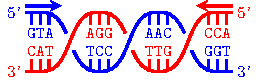
\includegraphics[width=\linewidth]{figures/tikz_dna.pdf}\\ DNA 双螺旋结构示意图，两条链分别以蓝色和红色表示。注意，螺旋中的序列彼此互补，且读取方向相反（从 5' 到 3'）。}
%{ (see Figure TODO (optional))}.
由于 DNA 分子总是从 $5'$ 端开始读取，而我们并不知道从哪一条链读取，因此像 ACCCTGG 这样的序列等价于将其反向并把每个字母替换为互补字母后得到的序列 CCAGGGT。
这称为字母序列的{\em 反向互补对称性}。
因此，我们得到二元素群 $\Z_2 = \{0, 1\}$，其中恒等变换对应于 $0$，反向互补变换对应于 $1$（复合运算满足 $1 + 1 = 0 \mod{2}$）。
完整的群结合了平移与反向互补变换。



在我们的情形中，
第 \ref{sec:groups} 节定义的群卷积~(\ref{eq:group-conv}) 可写为
%is defined as:
\begin{equation}
    (x \star \theta)(\fg) = \sum_{u \in \Omega} x_u \rho(\fg) \theta_u,
\end{equation}
它是（单通道）输入信号 $x$ 与滤波器 $\theta$ 的内积；滤波器由 $\fg \in \fG$ 通过 $\rho(\fg) \theta_u = \theta_{\fg^{-1} u}$ 进行变换，而输出 $x\star \theta$ 是 $\fG$ 上的函数。
注意，由于 $\Omega$ 是离散的，我们把式~(\ref{eq:group-conv}) 中的积分替换成了求和。%\michael{Define: what is the size of $\rho(\fg)$?} \petar{I think it depends on whether we're doing DNA conv or rotation conv.}


\paragraph{变换+卷积方法}
我们将说明，群卷积可以分两步实现：滤波器变换步骤和平移卷积步骤。
滤波器变换步骤为基本滤波器创建旋转（或反向互补变换）副本，而平移卷积与标准 CNN 中相同，因而可以在 GPU 等硬件上高效计算。%highly optimized.
为说明这一点，注意在两个例子中，我们都可以把一般变换 $\fg \in \fG$ 写成先进行变换 $\fh \in \fH$（例如旋转或反向互补变换），再进行平移 $\fk \in \Z^d$，即 $\fg = \fk \fh$（并置表示群元素 $\fk$ 和 $\fh$ 的复合）。
由群表示的性质，% $\rho$ is a representation,
可得 $\rho(\fg) = \rho(\fk \fh) = \rho(\fk) \rho(\fh)$。
因此，%we have
\begin{equation}
    \begin{aligned}
        (x\star \theta )(\fk \fh) 
        &=
        \sum_{u \in \Omega} x_u \rho(\fk) \rho(\fh) \theta_{u} \\
        &=
        \sum_{u \in \Omega} x_u (\rho(\fh) \theta)_{u - \fk}
    \end{aligned}
\end{equation}
%\michael{is the filter reversed here? }
可以看出，最后一个等式正是信号 $x$ 与变换后滤波器 $\rho(\fh) \theta$ 的标准（平面欧氏）卷积。
因此，为了对这些群实现群卷积，我们取规范滤波器 $\theta$，创建变换后的副本 $\theta_\fh = \rho(\fh) \theta$，每个 $\fh \in \fH$ 对应一个副本（例如每个旋转 $\fh \in O_h$ 或 DNA 反向互补对称性 $\fh \in \Z_2$），然后用 $x$ 分别与这些滤波器卷积：$(x\star \theta )(\fk \fh)  = (x\star \theta_{\fh} )(\fk)$。
在两个例子中，对称性都只是通过置换滤波器系数作用于滤波器，离散旋转的情形如图 \ref{fig:cayley-diagram-Oh} 所示。
因此，这些运算可以使用预先计算索引的索引操作高效实现。


尽管我们把群卷积 $x \star \theta$ 输出的特征图定义为 $\fG$ 上的函数，但由于 $\fg$ 可以分解为 $\fh$ 和 $\fk$，也可以把它们看作一组堆叠的欧氏特征图（有时称为\emph{定向通道}），每个滤波器变换/定向 $\fk$ 对应一个特征图。
例如，在第一个例子中，我们会为每个滤波器旋转（图 \ref{fig:cayley-diagram-Oh} 中的每个节点）关联一个特征图，该特征图通过
%translationally 
以传统平移意义对旋转后的滤波器进行卷积而得到。
因此，这些特征图仍可存储为 $W \times H \times C$ 数组，其中通道数 $C$ 等于独立滤波器的数量乘以变换 $\fh \in \fH$（例如旋转）的数量。

如第 \ref{sec:groups} 节所示，群卷积是等变的：$(\rho(\fg) x) \star \theta = \rho(\fg) (x \star \theta)$。
就定向通道而言，这意味着在 $\fh$ 的作用下，每个定向通道都会发生变换，而各定向通道本身也会被置换。
例如，若对图 \ref{fig:cayley-diagram-Oh} 中的每个变换关联一个定向通道，并施加绕 z 轴 $90$ 度的旋转（对应红色箭头），特征图就会按照红色箭头所示进行置换。
%
上述描述清楚表明，群卷积神经网络与传统 CNN 十分相似。
因此，第~\ref{sec:cnnsec} 节讨论的许多网络设计模式（例如残差网络）也可以与群卷积结合使用。




\paragraph{Fourier 域中的球面 CNN}
对于第~\ref{sec:groups} 节所见的球面连续对称群，可以使用适当的 Fourier 变换在谱域中实现卷积（提醒读者，$\mathbb{S}^2$ 上的卷积是 $\mathrm{SO}(3)$ 上的函数，因此要实现多层球面 CNN，需要在这两个域上都定义 Fourier 变换）。
%
%The analogy of the Fourier basis on 
{\em 球谐函数}是二维球面上的一组正交基，类似于由复指数函数构成的经典 Fourier 基。
%
在特殊正交群上，Fourier 基称为 {\em Wigner D-functions}。%
在这两种情形中，Fourier 变换（系数）都通过与基函数取内积来计算，并且卷积定理的对应形式成立：可以把 Fourier 变换逐元素相乘，从而在 Fourier 域中计算卷积。
%
此外，还存在类 FFT 算法，可高效计算 $\mathbb{S}^2$ 和 $\mathrm{SO}(3)$ 上的 Fourier 变换。更多细节见 \cite{cohen2018spherical}。



%On the $\mathrm{SO}(3)$ group, the Fourier decomposition takes the form 
%$$
%f(\mathbf{R}) = \sum_{l\geq 0} (2l+1) \sum_{i=-l}^{+l} \sum_{j=-l}^{+l} \hat{f}_{l,ij} D_{l,ij}(\mathbf{R})
%$$
%where the Fourier coefficients are defined as %inner products 
%$$
%\hat{f}_{l,ij} = \int_{\mathrm{SO}(3)} f(\mathbf{R}) \overline{D_{l,ij}(\mathbf{R})}\mathrm{d}\mathbf{R}. 
%$$
%The basis functions $D_{l,ij}(\mathbf{R})$ are called the {\em Wigner D-functions}, indexed by the degree $l\geq 0$ and order $i,j = -l, \hdots, +l$, and can be considered as complex matrix-valued functions $\mathbf{D}_l : \mathrm{SO}(2) \rightarrow \mathbb{C}^{(2l+1)\times (2l+1)}$. 
%% \paragraph{Steerability}
%





\subsection{图神经网络}\label{sec:gnn-intro}

%[MOVED from 1.3]

%since graphs exhibit less restrictive geometries and invariances, they invite for the most flexible class of architectures---the \emph{Graph Neural Networks} (GNN). As we will see, all of the neural architectures we will study in this book can be understood as a special case of the GNN, with injected additional geometric constraints and invariances.

%The general concept of constructing {\em permutation equivariant} functions operating over graphs as shared {\em permutation invariant} functions operating over local neighbourhoods appears to be very powerful and underlies the design of most Graph Neural Networks. Under various guises, this local function $g$ can be referred to as ``diffusion'', ``propagation'', or ``message passing''. 
%
%If we are interested in a graph-level output, a common recipe is to construct the latent node features using a {\em permutation equivariant} function $f$, followed by a {\em permutation invariant} function $h$ over the entries of $f({\bf X}, {\bf A})$ to obtain an ordering-independent output. In this context, the function $h$ is often referred to as ``readout'' or ``global pooling''.




%====

图神经网络（GNN）利用置换群的性质，在图上实现了我们的几何深度学习蓝图。GNN 是目前最一般的深度学习架构类别之一；正如本文将说明的，大多数其他深度学习架构都可以理解为带有额外几何结构的 GNN 特例。


按照第 \ref{sec:proto-graphs} 节的讨论，我们认为一个图由邻接矩阵 $\mathbf{A}$ 和节点特征 $\mathbf{X}$ 指定。
%
%
我们将研究如下 GNN 架构：它们是{\em 置换等变}函数 $\mathbf{F}(\mathbf{X},\mathbf{A})$，通过在局部邻域上应用共享的{\em 置换不变}函数 $\phi(\mathbf{x}_u, \mathbf{X}_{\mathcal{N}_u})$ 构造而成。在不同表述中，这一局部函数 $\phi$ 可称为“扩散”“传播”或“消息传递”，而这种 $\mathbf{F}$ 的整体计算则称为“GNN 层”。


在写作本文时，GNN 层的设计与研究是深度学习最活跃的领域之一，因而其研究版图难以梳理。所幸，我们发现绝大多数文献都可以从 GNN 层的三种“类型”（图 \ref{fig:gc_flavours}）推导出来，下面将予以介绍。这些类型决定了 $\phi$ 对邻域特征进行变换的程度，从而允许以不同复杂度建模图上的交互。


在这三种类型中，来自 $\vec{X}_{\mathcal{N}_u}$ 的特征（可能借助某个函数 $\psi$ 进行变换）会由置换不变函数 $\bigoplus$ 进行\emph{聚合}；随后，节点 $u$ 的特征由某个函数 $\phi$ {\em 更新}，从而保证置换不变性。通常，\marginnote{最常见的情形是，$\psi$ 和 $\phi$ 是带激活函数的可学习仿射变换；例如 $\psi(\vec{x}) = {\bf W}\vec{x} + \vec{b}$；$\phi(\vec{x}, \vec{z}) = \sigma\left({\bf W}\vec{x} + {\bf U}\vec{z} + \vec{b}\right)$，其中 ${\bf W}, {\bf U}, \vec{b}$ 是可学习参数，而 $\sigma$ 是修正线性单元等激活函数。$\vec{x}_u$ 作为 $\phi$ 的额外输入，表示一个可选的{\em 跳跃连接}，这通常非常有用。}$\psi$ 和 $\phi$ 是可学习的，
%$\fdef{\bigoplus}{\mathcal{P}(\mathbb{R}^k)}{\mathbb{R}^{k'}}$. 
%
而 $\bigoplus$ 则实现为求和、均值或最大值等非参数运算，不过也可以使用循环神经网络等方式构造 \citep{murphy2018janossy}。


\begin{figure}
    \centering
    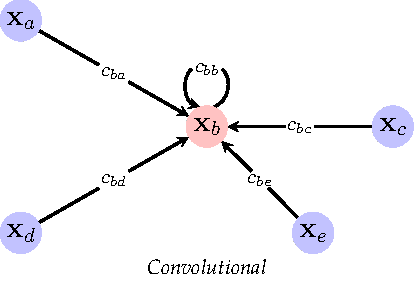
\includegraphics[width=0.33\linewidth]{figures/GNN_GDL_TYPES_C.pdf}
    \hspace{-0.5em}
    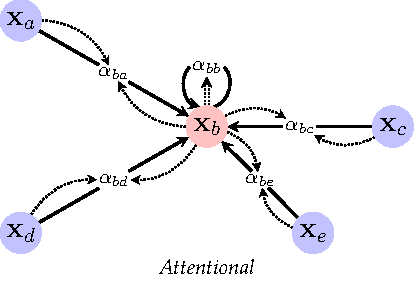
\includegraphics[width=0.33\linewidth]{figures/GNN_GDL_TYPES_A.pdf}
    \hspace{-0.5em}
    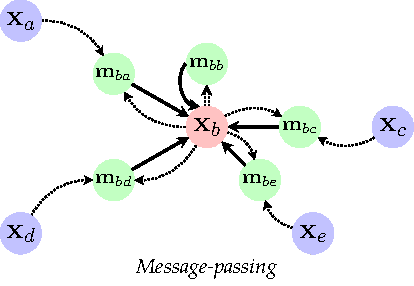
\includegraphics[width=0.33\linewidth]{figures/GNN_GDL_TYPES_MP.pdf}
    \caption{三种 GNN 层类型 $g$ 的数据流可视化。我们用图 \ref{fig:gc_gdl} 中节点 $b$ 的邻域加以说明。从左到右分别为：\textbf{卷积型}，其中发送节点特征乘以常数 $c_{uv}$；\textbf{注意力型}，其中该乘子通过接收节点对发送节点的注意力机制\emph{隐式}计算：$\alpha_{uv}=a(\vec{x}_u, \vec{x}_v)$；以及\textbf{消息传递型}，其中基于发送节点和接收节点共同计算向量消息：$\vec{m}_{uv}=\psi(\vec{x}_u, \vec{x}_v)$。}
    \label{fig:gc_flavours}
\end{figure}%

%All of the above considered, the three flavours are as follows (Figure \ref{fig:gc_flavours}):



%\begin{itemize}
%\item 
在\textbf{卷积型} \citep{kipf2016semi,defferrard2016convolutional,wu2019simplifying} 中，邻域节点的特征使用固定权重直接聚合：
\begin{equation}
    \vec{h}_u = \phi\left(\vec{x}_u, \bigoplus\limits_{v\in\mathcal{N}_u}c_{uv}\psi(\vec{x}_v)\right).
\end{equation}
这里，$c_{uv}$ 指定节点 $v$ 对节点 $u$ 表示的\emph{重要性}。它是一个常数，通常直接依赖于表示图结构的 ${\bf A}$ 中的元素。
%
注意，当聚合算子 $\bigoplus$ 取为求和时，可以将其视为线性扩散或位置相关的线性滤波，即卷积的推广。\marginnote{值得注意的是，这一类型并不能表示\emph{所有}卷积型（即与图结构可交换的）GNN 层，但涵盖了实践中提出的大多数此类方法。未来工作将给出详细讨论和扩展。}
%
具体而言，第~\ref{sec:manifolds} 节和第~\ref{sec:meshes} 节所见的谱滤波器属于这一类别，因为它们相当于对逐节点信号应用固定局部算子（例如 Laplacian 矩阵）。
 
 
%\michael{Now we discussed spectral filters, so we can add a remark here}

%\item 
在\textbf{注意力型} \citep{velickovic2018graph,monti2017geometric,zhang2018gaan} 中，交互是隐式的：
\begin{equation}
    \vec{h}_u = \phi\left(\vec{x}_u, \bigoplus\limits_{v\in\mathcal{N}_u}a(\vec{x}_u, \vec{x}_v)\psi(\vec{x}_v)\right).
\end{equation}
这里，$a$ 是可学习的\emph{自注意力机制}，用于隐式计算重要性系数 $\alpha_{uv} = a(\vec{x}_u, \vec{x}_v)$。这些系数通常在所有邻居上进行 softmax 归一化。
%
当 $\bigoplus$ 为求和时，聚合结果仍是邻域节点特征的线性组合，但此时权重依赖于特征。


%\item 
最后，\textbf{消息传递型} \citep{gilmer2017neural,battaglia2018relational} 相当于沿边计算任意向量（“消息”）：
\begin{equation}
    \vec{h}_u = \phi\left(\vec{x}_u, \bigoplus\limits_{v\in\mathcal{N}_u}\psi(\vec{x}_u, \vec{x}_v)\right).
\end{equation}
这里，$\psi$ 是可学习的\emph{消息函数}，用于计算节点 $v$ 发送给节点 $u$ 的向量；聚合则可以视为图上的一种消息传递形式。
%\end{itemize}


需要注意的是，这些方法在表示能力上存在包含关系：\emph{卷积} $\subseteq$ \emph{注意力} $\subseteq$ \emph{消息传递}。事实上，注意力型 GNN 可以用实现为查找表 $a(\vec{x}_u, \vec{x}_v) = c_{uv}$ 的注意力机制来表示卷积型 GNN；而卷积型和注意力型 GNN 都是消息传递的特例，其中消息仅包含发送节点的特征：对于卷积型 GNN，$\psi(\vec{x}_u, \vec{x}_v) = c_{uv}\psi(\vec{x}_v)$；对于注意力型 GNN，$\psi(\vec{x}_u, \vec{x}_v) = a(\vec{x}_u, \vec{x}_v)\psi(\vec{x}_v)$。
%

这并不意味着消息传递型 GNN 始终是最有用的变体；由于它们必须沿边计算向量值消息，通常更难训练，并且需要庞大的内存。此外，在许多自然产生的图上，图的边编码了下游类别的相似性（即一条边 $(u, v)$ 意味着 $u$ 和 $v$ 很可能具有相同输出）。对于这种图（常称为\emph{同配图}），无论从正则化还是可扩展性看，在邻域上进行卷积聚合通常都是远为合适的选择。注意力型 GNN 提供了一个“中间方案”：它们能够对邻域内的复杂交互进行建模，同时沿边仅计算标量值，因此比消息传递型更具可扩展性。


这里提出“三种类型”的分类是为了保持简洁，因而不可避免地忽略了 GNN 模型中大量细微差别、洞见、推广和历史背景。尤其是，它不包括基于 Weisfeiler-Lehman 层次结构的高维 GNN，以及依赖显式计算图 Fourier 变换的谱%\marginnote{Though many works make a distinction between ``spatial'' and ``spectral'' GNNs, we find that this distinction is rather artificial and must be taken with a grain of salt. Many proposed spectral filters are expressible in terms of simple matrix operations (e.g. polynomials of the graph Laplacian) and hence boil down to simple spatial operations that fall under the ``convolutional'' flavor presented here.}
GNN。
%
%Such a wealth somewhat uniquely appears in graph representation learning, given the flexible invariances present in graphs, and their ubiquity as a representational tool across the natural and social sciences. 
%We will dedicate Chapter \ref{ch:graphs} to a more careful and detailed exploration of deep learning models for graphs.

%\marginnote{Examples to be covered include: higher-order GNNs, $k$-invariant graph networks, and ``true spectral'' GNNs which rely on the Graph Fourier Transform.}




%We now provide a ``bird's eye'' view of \emph{graph neural networks} (GNNs)---the most popular approach for constructing permutation equivariant neural models over graphs.

%As per Section \ref{sec:proto-graphs}, we will consider a graph  representation learning setup with graphs specified by a matrix of node features, ${\bf X}\in\mathbb{R}^{|V|\times k}$ and an adjacency matrix, ${\bf A}\in\mathbb{R}^{|V|\times |V|}$. Our aim is to construct permutation equivariant functions over these graphs, $\fdef{f}{\mathbb{R}^{|V|\times k} \times \mathbb{R}^{|V|\times |V|}}{\mathbb{R}^{|V|\times k'}}$, such that $f({\bf X}, {\bf A}) = {\bf H}$, where $\vec{x}_i$ and $\vec{h}_i$ are the input and latent features of node $i$. 

%Furthermore, we will construct $f$ through shared application of a local function, $\fdef{g}{\mathbb{R}^k\times \mathcal{P}(\mathbb{R}^k)}{\mathbb{R}^{k'}}$, such that $g(\vec{x}_i, \vec{X}_{\mathcal{N}_i}) = \vec{h}_i$, where $\vec{X}_{\mathcal{N}_i}\in\mathcal{P}(\mathbb{R}^k)$ is a set of features of nodes that neighbour $i$. If $g$ is permutation invariant with respect to $\mathcal{N}_i$, it guarantees permutation equivariance of $f$. For the purposes of this section, we will refer to $g$ as a \emph{GNN layer}.

%The design and study of GNN layers is one of the most active areas of deep learning at the time of writing, making it a landscape that is challenging to navigate. Fortunately, we find that the vast majority of the literature may be derived from only three ``flavours'' of \emph{spatial}\marginnote{Several influential works partition GNNs into \emph{spatial} and \emph{spectral}. Despite the apparent divide, our spatially-focused discussion in this section encompasses many proposed spectral approaches as well. In order to derive efficient implementations, spectral GNNs often ``spatialise'' themselves, using a polynomial expansion of the adjacency information. We will provide a thorough treatment of the spectral direction in Chapter \ref{ch:graphs}.} GNN layers, which we will present here. These flavours govern the extent to which $g$ transforms the features in $\mathcal{N}_i$, allowing for varying degrees of complexity when modelling interactions across the graph.

%In all three flavours, permutation invariance is ensured by \emph{aggregating} (potentially transformed) features from $\vec{X}_{\mathcal{N}_i}$ with a permutation-invariant function, which we will denote by $\fdef{\bigoplus}{\mathcal{P}(\mathbb{R}^k)}{\mathbb{R}^{k'}}$. Usually, $\bigoplus$ is realised as a nonparametric operation such as elementwise-sum or maximisation, but it may be constructed by carefully leveraging permutation-sensitive parametric functions such as recurrent neural networks \citep{murphy2018janossy}.

%All of the above considered, the three flavours are as follows (Figure \ref{fig:gc_flavours}):

%\begin{itemize}
%\item The \textbf{convolutional} flavour, directly aggregating neighbourhoods:

%\begin{equation}
%    \vec{h}_i = \phi\left(\vec{x}_i, \bigoplus\limits_{j\in\mathcal{N}_i}c_{ij}\psi(\vec{x}_j)\right)
%\end{equation}
%Here, $\psi$ and $\phi$ are learnable transformations\marginnote{Most commonly, $\psi$ and $\phi$ are learnable affine transformations with activation functions; e.g. $\psi(\vec{x}) = {\bf W}\vec{x} + \vec{b}$; $\phi(\vec{x}, \vec{z}) = \sigma\left({\bf W}\vec{x} + {\bf U}\vec{z} + \vec{b}\right)$, where ${\bf W}, {\bf U}, \vec{b}$ are learnable parameters and $\sigma$ is an activation function such as the rectified linear unit. The additional input of $\vec{x}_i$ to $\phi$ represents an optional skip-connection, which is often very useful.}, and $c_{ij}$ specifies the \emph{importance} of node $j$ to node $i$'s representation. It is a constant that often directly depends on the entries in ${\bf A}$.
%
%\item The \textbf{attentional} flavour, where interaction constants are implicit:
%\begin{equation}
%    \vec{h}_i = \phi\left(\vec{x}_i, \bigoplus\limits_{j\in\mathcal{N}_i}a(\vec{x}_i, \vec{x}_j)\psi(\vec{x}_j)\right)
%\end{equation}
%Here, $\fdef{a}{\mathbb{R}^k\times\mathbb{R}^k}{\mathbb{R}}$ is a learnable \emph{self-attention mechanism}  that computes the importance coefficients $\alpha_{ij} = a(\vec{x}_i, \vec{x}_j)$ implicitly. They are often softmax-normalised across all neighbours.
%
%\item The \textbf{message-passing} flavour, computing arbitrary vectors across edges:
%\begin{equation}
%    \vec{h}_i = \phi\left(\vec{x}_i, \bigoplus\limits_{j\in\mathcal{N}_i}\psi(\vec{x}_i, \vec{x}_j)\right)
%\end{equation}
%Here, $\psi$ is a learnable \emph{message function}, computing $j$'s vector sent to $i$.
%\end{itemize}
%
%
%One important thing to note is a representational containment between these approaches: \emph{convolution} $\subseteq$ \emph{attention} $\subseteq$ \emph{message-passing}. Indeed, attentional GNNs can represent convolutional GNNs by an attention mechanism implemented as a \emph{look-up table}: $a(\vec{x}_i, \vec{x}_j) = c_{ij}$, and both convolutional and attentional GNNs are special cases of message-passing where the messages are only the sender nodes' features: $\psi(\vec{x}_i, \vec{x}_j) = c_{ij}\widetilde{\psi}(\vec{x}_j)$ for convolutional GNNs and $\psi(\vec{x}_i, \vec{x}_j) = a(\vec{x}_i, \vec{x}_j)\widetilde{\psi}(\vec{x}_j)$ for attentional GNNs.
%
%This does not imply that message passing GNNs are always the most useful variant; as they have to compute vector-valued messages across edges, they are typically harder to train and require unwieldy amounts of memory. Further, on a wide range of naturally-occurring graphs, the graph's edges encode for downstream class similarity (i.e. an edge $(i, j)$ implies that $i$ and $j$ are likely to have the same output). For such graphs (often called \emph{homophilous}), convolutional aggregation across neighbourhoods is often a far better choice, both in terms of regularisation and scalability. Attentional GNNs offer a ``middle-ground'': they allow for modelling complex interactions within neighbourhoods while computing only scalar-valued quantities across the edges, making them more scalable than message-passing.
%
%The categorisation presented here is provided with brevity in mind. It necessarily neglects a wealth of nuances, insights, generalisations and historical contexts to GNN models.\marginnote{Examples to be covered include: higher-order GNNs, $k$-invariant graph networks, and ``true spectral'' GNNs which rely on the Graph Fourier Transform.} Such a wealth somewhat uniquely appears in graph representation learning, given the flexible invariances present in graphs, and their ubiquity as a representational tool across the natural and social sciences. We will dedicate Chapter \ref{ch:graphs} to detailedly expanding on this analysis, and graph representation learning more generally.
 

\subsection{Deep Sets、Transformer 与潜在图推断}
\label{sec:deepset}

我们以用于学习\emph{无序集合}表示的置换等变神经网络架构结束对 GNN 的讨论。虽然集合在本文讨论的各类域中结构最少，但 Transformer \citep{vaswani2017attention} 和 Deep Sets \citep{zaheer2017deep} 等广受欢迎的架构最近凸显了它们的重要性。
%
%correspond to the least-restrictive geometry, these ``set neural networks'' have risen to high prominence recently: especially through the Deep Sets \citep{zaheer2017deep} and Transformer \citep{vaswani2017attention} architectures. 
%
使用第 \ref{sec:proto-graphs} 节的语言，我们假设给定节点特征矩阵 ${\bf X}$，但没有指定节点间的邻接或次序信息。具体架构取决于对节点之间\emph{交互}进行建模的程度。
 
\paragraph*{空边集}

%On the surface, 
无序集合不附带任何额外结构或几何，因此可以认为，处理它们最自然的方法是完全\emph{独立地}对待每个集合元素。这对应于此类输入上的置换等变函数，第 \ref{sec:proto-graphs} 节已经介绍过它：对每个节点分别应用一个共享变换。沿用描述 GNN 时的记号（第 \ref{sec:gnn-intro} 节），此类模型可以表示为
\begin{equation*}
    \vec{h}_u = \psi(\vec{x}_u),
\end{equation*}
其中 $\psi$ 是可学习变换。可以看出，这是满足 $\mathcal{N}_u = \{u\}$ 的卷积型 GNN 特例；等价地，${\bf A} = {\bf I}$。为肯定 \cite{zaheer2017deep} 从理论上证明此类架构若干通用逼近性质的工作，这种架构通常称为 Deep Sets。需要注意的是，在计算机视觉和图形学中处理\emph{点云}时经常需要处理无序集合；在这一领域，此类模型称为 PointNet \citep{qi2017pointnet}。



\paragraph*{完全边集}%: Self-attention and Transformers}

虽然假设空边集是构造无序集合上函数的一种高效方式，但我们通常会预期集合元素表现出某种关系结构，即节点之间存在一个\emph{潜在图}。令 ${\bf A} = {\bf I}$ 会丢弃所有这类结构，并可能导致次优性能。
%
反过来，可以假设在没有任何其他先验知识时，我们无法预先排除节点之间的\emph{任何}可能连接。在这种方法中，我们假设图是\emph{完全图}，${\bf A} = {\bf 1}{\bf 1}^\top$；等价地，$\mathcal{N}_u = \mathcal{V}$。
%
由于我们假设无法获得任何交互系数，在这种图上运行{\em 卷积型} GNN 相当于：
\begin{equation*}
\vec{h}_u = \phi\left(\vec{x}_u, \bigoplus_{v\in \mathcal{V}} \psi(\vec{x}_v)\right),
\end{equation*}
其中第二个输入 $\bigoplus_{v\in \mathcal{V}} \psi(\vec{x}_v)$ 对所有节点 $u$ 都\emph{相同}\marginnote{这是 $\bigoplus$ 的置换不变性所产生的直接结果。}，因此模型的表示能力与完全忽略该输入时等价，也就是上文提到的 ${\bf A} = {\bf I}$ 情形。

这促使我们使用表示能力更强的 GNN 类型，即{\em 注意力型}：
\begin{equation}
    \vec{h}_u = \phi\left(\vec{x}_u, \bigoplus_{v\in \mathcal{V}} a(\vec{x}_u, \vec{x}_v)\psi(\vec{x}_v)\right)
\end{equation}
这会得到\emph{自注意力}算子，即 Transformer 架构的核心 \citep{vaswani2017attention}。假设对注意力系数进行某种归一化（例如 softmax），便可将所有标量 $a(\vec{x}_u, \vec{x}_v)$ 约束在范围 $[0, 1]$ 内；因此，可以把自注意力看作推断一个\emph{软邻接矩阵} $a_{uv} = a(\vec{x}_u, \vec{x}_v)$，它是针对某个下游任务进行基于梯度优化的副产物。

上述视角意味着，我们可以把 Transformer 精确表述为完全图上的注意力型 GNN \citep{joshi2020transformers}。\marginnote{采用消息传递型也同样合适。
%to complete graphs, yielding:
%\begin{equation}
%    \vec{h}_i = \phi\left(\vec{x}_i, \bigoplus_{j\in %V}\psi(\vec{x}_i, \vec{x}_j)\right)
%\end{equation}
虽然消息传递型在物理模拟和关系推理中很流行（例如 \cite{battaglia2016interaction,santoro2017simple}），但其应用不如 Transformer 广泛。这很可能是因为在完全图上计算向量消息会带来内存问题，或者因为基于向量的消息不如自注意力给出的“软邻接”容易解释。}然而，这与 Transformer 最初为建模\emph{序列}而提出这一事实存在表面冲突：$\vec{h}_u$ 的表示应考虑节点 $u$ 在序列中的\emph{位置}，而完全图聚合会忽略该位置。Transformer 通过引入\emph{位置编码}来解决这一问题：扩充节点特征 $\vec{x}_u$，使其编码节点 $u$ 在序列中的位置，通常取为频率依赖于 $u$ 的正弦波采样值。

在不存在节点自然次序的图上，人们为这种位置编码提出了多种替代方案。我们把这些方案留待后文讨论，但指出一个很有前景的方向：Transformer 中使用的位置编码可以直接关联到离散 Fourier 变换（DFT），继而关联到“环形网格”的图 Laplacian 特征向量。因此，Transformer 的位置编码隐式表示了输入节点按网格连接这一假设。对于更一般的图结构，可以直接使用（假设的）图之 Laplacian 特征向量；\citet{dwivedi2020generalization} 在其经验性能强大的 Graph Transformer 模型中利用了这一观察。
%\michael{add citations and briefly discuss?}
%; we defer this discussion to Chapter \ref{ch:graphs}. 


\paragraph*{推断的边集}

最后，可以尝试学习潜在关系结构，从而得到某个一般的 ${\bf A}$，它既不是 ${\bf I}$，也不是 ${\bf 1}{\bf 1}^\top$。为 GNN 推断潜在邻接矩阵 ${\bf A}$ 的问题（常称为\emph{潜在图推断}）在图表示学习中备受关注。这是因为假设 ${\bf A} = {\bf I}$ 可能在表示能力上较弱，而 ${\bf A} = {\bf 1}{\bf 1}^\top$ 又可能由于内存需求和需要聚合的大邻域而难以实现。此外，它也最接近“真正的”问题：推断邻接矩阵 ${\bf A}$ 意味着检测 ${\bf X}$ 各行之间的有用结构，进而可能有助于提出变量间因果关系等假设。

遗憾的是，这种表述必然会增加建模复杂度。具体而言，它要求在结构学习目标（该目标是\emph{离散的}，因而难以进行基于梯度的优化）与使用该图的下游任务之间取得恰当平衡。这使潜在图推断成为一个极具挑战且错综复杂的问题。%, and as such, we will defer thoroughly discussing it to Chapter \ref{ch:graphs}.

\subsection{等变消息传递网络}

在图神经网络的许多应用中，节点特征（或其中一部分）并非任意向量，而是几何实体的\emph{坐标}。例如，在处理分子图时，表示原子的节点可能同时包含原子类型和三维空间坐标信息。我们希望后一部分特征的变换方式与分子在空间中的变换方式相同；换言之，除了前文讨论的标准置换等变性外，还应对由刚性运动（旋转、平移和反射）组成的欧氏群 $\mathrm{E}(3)$ 具有等变性。

为开展下面（略作简化的）分析，我们区分节点{\em 特征} $\mathbf{f}_u \in \mathbb{R}^d$ 和节点{\em 空间坐标} $\mathbf{x}_u\in \mathbb{R}^3$；后者带有欧氏对称结构。在这一设定下，等变层会显式、分别地变换这两类输入，得到修改后的节点特征 $\vec{f}'_u$ 和坐标 $\vec{x}'_u$。

现在可以按照几何深度学习蓝图陈述所需的等变性质。若输入的空间分量由 $\fg\in \mathrm{E}(3)$ 变换（表示为 $\rho(\fg)\mathbf{x} = \mathbf{R}\mathbf{x} + \mathbf{b}$，其中 $\mathbf{R}$ 是建模旋转与反射的正交矩阵，$\mathbf{b}$ 是平移向量），则输出的空间分量以相同方式变换（即 $\mathbf{x}'_u \mapsto \mathbf{R}\mathbf{x}'_u + \mathbf{b}$），而 $\mathbf{f}'_u$ 保持不变。

与前文在一般图语境下讨论的置换等变函数空间类似，满足上述约束的 $\mathrm{E}(3)$ 等变层数量极多，但并非所有这类层都具有几何稳定性或易于实现。事实上，实际有用的等变层空间很可能可以用一种简单分类来描述，类似于空间 GNN 层的“三种类型”。
%
\cite{satorras2021n} 以{\em 等变消息传递}的形式提出了一种优雅的解决方案。其模型运作如下：
%GNN by . In their model, a distinction is made between node {\em features} $\mathbf{f}_u \in \mathbb{R}^s$ and node {\em spatial coordinates} $\mathbf{x}_u\in \mathbb{R}^3$; the latter are endowed with Euclidean symmetry structure. 
%
%Equivariant message passing 
%can be expressed as 
\begin{eqnarray*}
    \vec{f}'_u &=& \phi\left(\vec{f}_u, \bigoplus\limits_{v\in\mathcal{N}_u}\psi_\mathrm{f}(\vec{f}_u, \vec{f}_v, \| \vec{x}_u - \vec{x}_v \|^2)\right), \\
    %
        %
    \vec{x}'_u &=& \mathbf{x}_u + \sum_{v\neq u} (\vec{x}_u - \vec{x}_v) \psi_\mathrm{c}(\vec{f}_u, \vec{f}_v, \| \vec{x}_u - \vec{x}_v \|^2)
\end{eqnarray*}
%
其中 $\psi_\mathrm{f}$ 和 $\psi_\mathrm{c}$ 是两个不同的（可学习）函数。可以证明，这种聚合在空间坐标的欧氏变换下是等变的。这是因为 $\mathbf{f}'_u$ 对 $\mathbf{x}_u$ 的依赖仅通过距离 $\| \vec{x}_u - \vec{x}_v \|^2$ 体现，而 $\mathrm{E}(3)$ 的作用必然保持节点间距离不变。此外，这类层的计算可以视为“消息传递型”GNN 的一个特例，因此易于高效实现。

总之，与普通 GNN 不同，\cite{satorras2021n} 能够正确处理图中每个点的“坐标”。这些坐标现在被视为 $\mathrm{E}(3)$ 群的成员，这意味着当输入发生旋转、反射和平移时，网络输出具有正确的行为。\marginnote{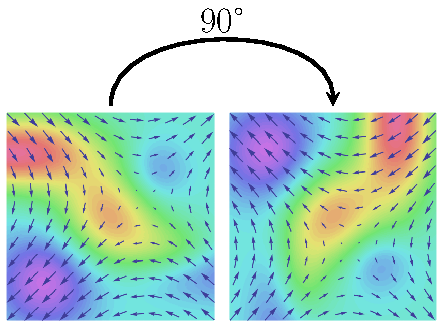
\includegraphics[width=\linewidth]{figures/rotate.pdf}\\ 标量特征（热图）在旋转下不发生变化，而向量特征（箭头）可能改变方向。前述简单的 $\mathrm{E}(3)$ 等变 GNN 没有考虑这一点。}然而，特征 $\vec{f}_u$ 仍按通道处理，并继续假设为在这些变换下不发生变化的\emph{标量}。
%
这限制了该框架能够捕获的空间信息类型。例如，我们可能希望把某些特征编码为\emph{向量}，如点的速度；这些向量在上述变换下\emph{应当}改变方向。
\cite{satorras2021n} 在其架构的一个变体中引入速度概念，部分缓解了这一问题。速度是每个点的一种三维向量属性，会随之正确旋转。然而，这只是 $\mathrm{E}(3)$ 等变网络能够学习的一般表示中的一个很小子空间。一般而言，节点特征可以编码任意维度的\emph{张量}，这些张量仍按照 $\mathrm{E}(3)$ 以明确定义的方式变换。

因此，尽管上述架构已经为许多实际输入表示提供了优雅的等变解决方案，在某些情况下仍有必要探索更广泛的等变函数集合。处理此类设定的现有方法可以分为两类：\emph{不可约表示}（前述层是其简化实例）和\emph{正则表示}。这里仅作简要综述，详细讨论留待未来工作。

\paragraph{不可约表示}
不可约表示建立在如下结论之上：旋转平移群的所有元素都可以化为不可约形式，即由块对角矩阵旋转的向量。关键是，每个块都是一个 \emph{Wigner D-matrix}（即前述球面 CNN 的 Fourier 基）。这类方法使用等变核从一组不可约表示映射到另一组不可约表示。为找出完整的等变映射集合，可以直接求解这些核上的等变约束。所得解是等变基矩阵的线性组合，而这些基矩阵由{\em Clebsch-Gordan 矩阵}和球谐函数导出。

不可约表示方法的早期实例包括 Tensor Field Networks \citep{thomas2018tensor} 和 3D Steerable CNN \citep{weiler20183d}，二者都是在点云上运行的卷积模型。\citet{fuchs2020se} 的 $\mathrm{SE}(3)$-Transformer 使用注意力层而非卷积层，将这一框架扩展到图域。此外，尽管我们的讨论集中于 \citet{satorras2021n} 的特例解，但需要指出，在图上进行旋转或平移等变预测的动机在历史上也曾由其他领域探索，包括用于点云的 Dynamic Graph CNN \citep{wang2019dynamic}，以及用于量子化学的高效消息传递模型，如 SchNet \citep{schutt2018schnet} 和 DimeNet \citep{klicpera2020directional}。

\paragraph{正则表示}
不可约表示方法虽然很有吸引力，却要求直接对底层群表示进行推理，这可能十分繁琐，而且只适用于紧群。正则表示方法更加一般，但会带来额外计算负担——为实现精确等变性，它们需要为\emph{所有}群元素存储潜在特征嵌入的副本\marginnote{事实上，前面各节介绍的群卷积神经网络开创了这一方法。}。

这一领域有一种很有前景的方法，旨在通过指数映射和对数映射的定义考察对 \emph{Lie 群}的等变性，并有望在各种对称群上实现快速原型设计。Lie 群超出了本节范围，读者可参阅这一方向近期两个成功实例：\citet{finzi2020generalizing} 的 LieConv 和 \citet{hutchinson2020lietransformer} 的 LieTransformer。

本节介绍的方法代表了处理几何图上数据的流行方式，并对底层几何具有显式等变性。正如第~\ref{sec:meshes} 节所讨论的，\emph{网格}是几何图的一种特殊实例%， in a way that gives explicit semantics to the \emph{surface} spanned between the nodes.
，可以理解为连续曲面的离散化。
下面将研究网格专用的等变神经网络。


\subsection{内蕴网格 CNN}
网格，尤其是三角网格，是计算机图形学的基本工具，或许也是建模三维对象最常见的方式。深度学习总体上的显著成功，特别是 CNN 在计算机视觉中的成功，使图形学和几何处理社群在 2010 年代中期前后产生了浓厚兴趣\marginnote{
%If $v$ is local, such a description is unique. 
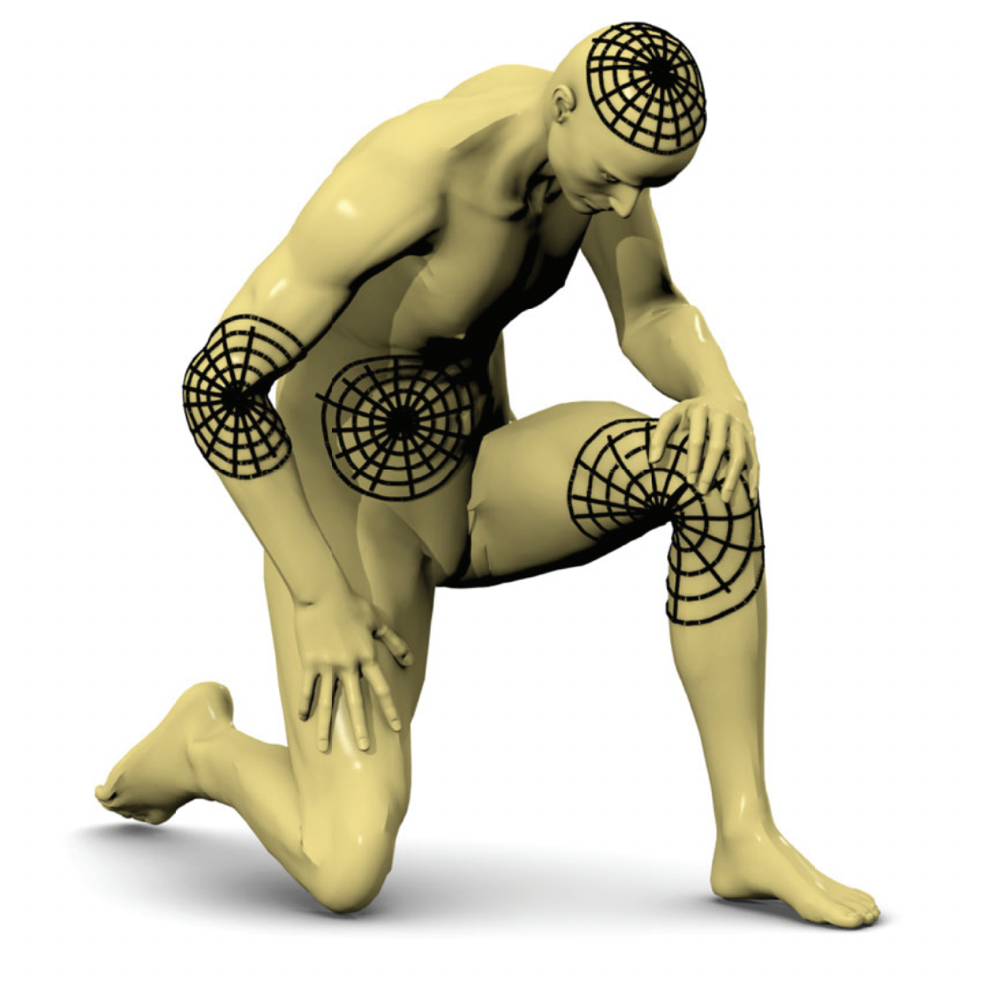
\includegraphics[width=0.9\linewidth]{figures/geo_patch.png}
测地斑块的例子。为使所得斑块成为拓扑圆盘，其半径 $R$ 必须小于单射半径。}，希望为网格数据构建类似架构。


\paragraph{测地斑块}
大多数网格深度学习架构通过
离散化或近似指数映射，并在切平面的坐标系中表示滤波器，来实现形式为~(\ref{eqn:conv_exp}) 的卷积滤波器。
%
发射一条测地线 $\gamma:[0,T]\rightarrow \Omega$，使其从一点 $u=\gamma(0)$ 到达邻近点 $v=\gamma(T)$，可定义一个局部{\em 测地极坐标}系 $(r(u,v),\vartheta(u,v))$，其中 $r$ 是 $u$ 与 $v$ 之间的测地距离（测地线 $\gamma$ 的长度），而 $\vartheta$ 是 $\gamma'(0)$ 与某一局部参考方向之间的夹角。% $X_0(u)$.
%(both tangent vectors in $T_u\Omega$). 
%
由此可以定义{\em 测地斑块} $x(u,r,\vartheta) = x(\exp_u \tilde{\omega}(r,\vartheta))$，其中 $\tilde{\omega}_u: [0,R]\times [0,2\pi) \rightarrow T_u\Omega$ 是局部极坐标标架。




在\marginnote{
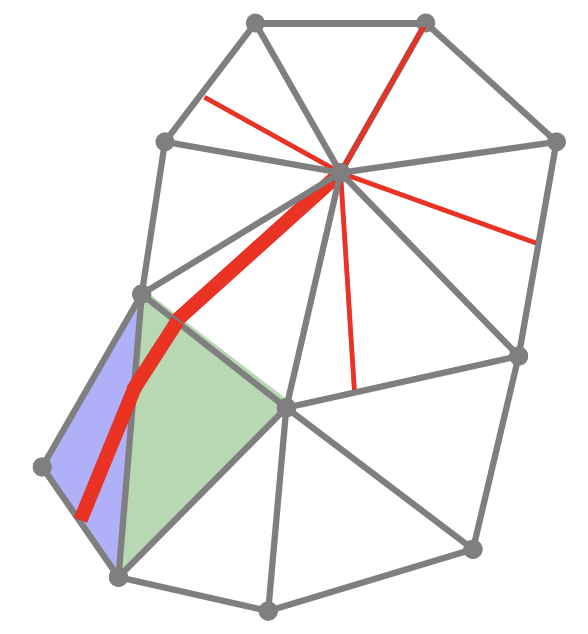
\includegraphics[width=0.9\linewidth]{figures/fmm.png}
网格上离散测地线的构造。}离散化为网格的曲面上，测地线是穿过三角形面的折线。传统上使用 Fast Marching 算法 \cite{kimmel1998computing} 计算测地线；该算法对介质中波传播物理模型里出现的一类非线性 PDE——{\em 程函方程}——进行高效数值近似。\cite{kokkinos2012intrinsic} 调整了这一方案以计算局部测地斑块，随后 \cite{masci2015geodesic} 再次使用它构建{\em Geodesic CNN}，这是首个网格上的内蕴类 CNN 架构。


\paragraph{各向同性滤波器}
重要的是，在测地斑块的定义中，参考方向和斑块定向的选择存在歧义。这恰好就是规范选择的歧义；我们的局部坐标系在相差任意旋转（或角坐标的平移 $x(u,r,\vartheta+\vartheta_0)$）的意义下定义，而该旋转在每个节点处都可能不同。
%
或许最直接的解决方案是使用形式为 $\theta(r)$ 的各向同性滤波器，它以方向无关的方式聚合邻居特征：
$$
(x\star \theta)(u) = \int_0^R \int_0^{2\pi} x(u,r,\vartheta) \theta(r) \mathrm{d}r \mathrm{d}\vartheta.
$$
第~\ref{sec:manifolds}--\ref{sec:meshes} 节讨论的谱滤波器属于这一类别：它们基于各向同性的 Laplacian 算子。
%
然而，这种方法会丢弃重要的方向信息，并且可能无法提取类边缘特征。


\paragraph{固定规范}
另一种方法是{\em 固定某个规范}，第~\ref{sec:manifolds} 节已经提到这一点。\cite{monti2017geometric} 使用主曲率方向：虽然这一选择不是内蕴的，并且在平坦点（曲率为零处）或曲率均匀处（如完美球面上）可能存在歧义，但作者
证明它适合处理近似分片刚性的可变形人体形状。
%
后续工作（例如 \cite{melzi2019gframes}）给出了网格上规范的可靠内蕴构造，即计算内蕴函数的（内蕴）梯度。虽然这类切向量场可能存在奇点（即在某些点处为零），但整个过程对噪声和重新网格化都非常稳健。


\paragraph{角向池化}
\cite{masci2015geodesic} 使用了另一种称为{\em 角向最大池化}的方法。在这种情况下，滤波器 $\theta(r,\vartheta)$ 是各向异性的，但它会在{\em 所有可能的旋转}上与函数进行匹配，随后聚合匹配结果：
$$
(x\star \theta)(u) = \max_{\vartheta_0 \in [0,2\pi) } \,\, \int_0^R \int_0^{2\pi} x(u,r,\vartheta) \theta(r,\vartheta+\vartheta_0) \mathrm{d}r \mathrm{d}\vartheta.
$$
从概念上看，可以将其可视化为用旋转滤波器与测地斑块进行相关运算，并收集最强响应。



%\michael{TBD: discrete}


在网格上，连续积分可以利用一种称为
{\em 斑块算子} \citep{masci2015geodesic} 的构造进行离散化。在节点 $u$ 周围的测地斑块中，邻居节点 $\mathcal{N}_u$\marginnote{通常使用多跳邻居。}在局部极坐标中表示为 $(r_{uv}, \vartheta_{uv})$，并由一组权重函数 $w_1(r,\vartheta), \hdots, w_K(r,\vartheta)$ 加权和聚合（如图~\ref{fig:patches} 所示，它们充当“软像素”）：
%locally aggregating the neighbout node features, 
$$
(x\star \theta)_u = \frac{
\sum_{k=1}^K w_{k} \sum_{v\in \mathcal{N}_u} (r_{uv},\vartheta_{uv}) x_v \, \theta_k
}
{
\sum_{k=1}^K w_{k} \sum_{v\in \mathcal{N}_u} (r_{uv},\vartheta_{uv}) \theta_k
}
$$
  %
  （这里%$x_j$ is the feature at node $j$ and
  $\theta_1,\hdots, \theta_K$ 是滤波器的可学习系数）。多通道特征按通道处理，并配备一族适当的滤波器。
  \cite{masci2015geodesic,boscaini2016learning} 使用预定义权重函数 $w$，而 \cite{monti2017geometric} 进一步允许这些函数可学习。
%




\begin{figure}[h!]
    \centering
    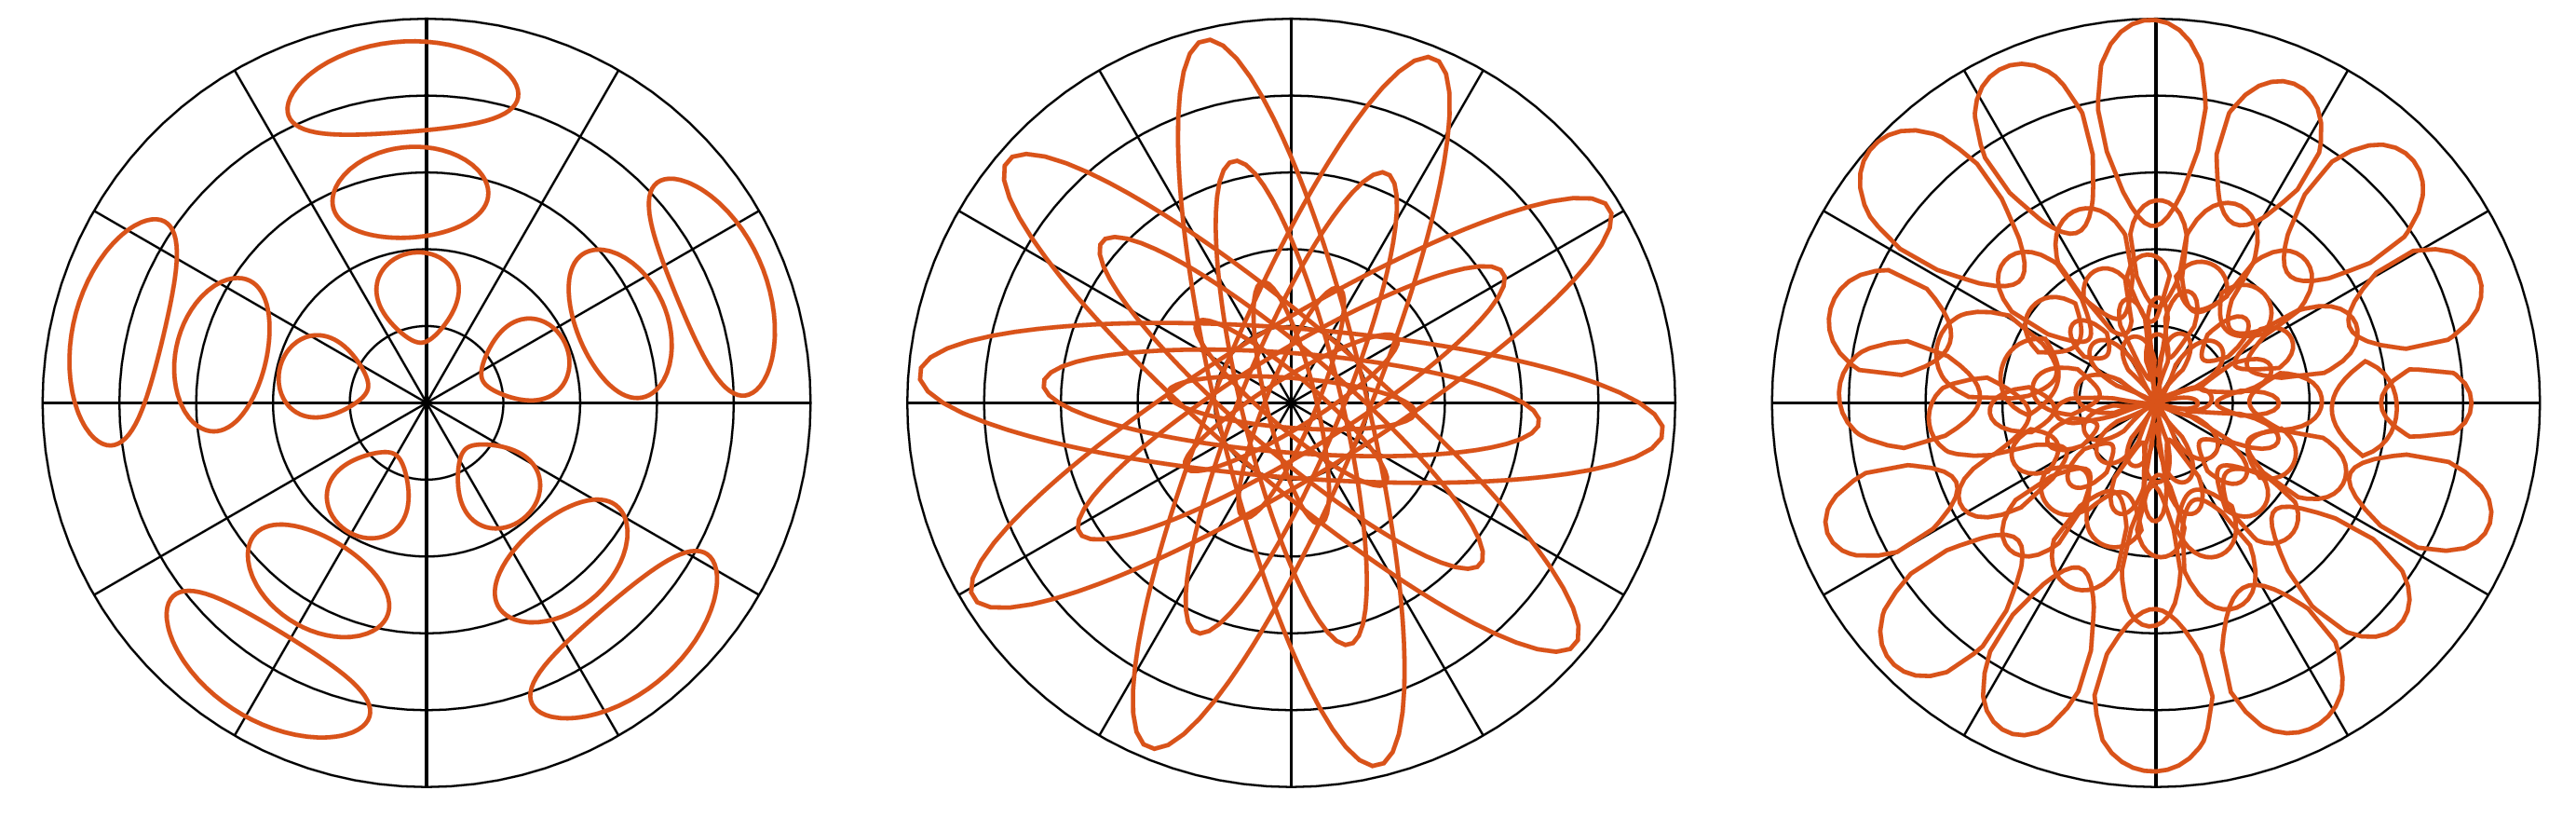
\includegraphics[width=\linewidth]{figures/patch.png}
    \caption{从左到右：Geodesic CNN \citep{masci2015geodesic}、Anisotropic CNN \citep{boscaini2016anisotropic} 和 MoNet \citep{monti2017geometric} 中使用的斑块算子示例，其中权重函数 $w_k(r,\vartheta)$ 的水平集以红色表示。
    }
    \label{fig:patches}
\end{figure}%


%\taco{Since this part of the paper is more focussed on implementation aspects, should we explain how the integrals above are actually evaluated? i.e. how to approximate this one a mesh.}



\paragraph{规范等变滤波器}
各向同性滤波器和角向最大池化都会产生对规范变换{\em 不变}的特征；它们按照平凡表示 $\rho(\fg) = 1$ 进行变换（其中 $\fg \in \mathrm{SO}(2)$ 是局部坐标标架的旋转）。
这一观点启发了 \cite{cohen2019gauge, deHaan2020gauge} 提出的另一种方法，第~\ref{sec:gauges} 节对此进行了讨论。在该方法中，网络计算的特征与任意表示 $\rho$ 相关联，而该表示属于结构群 $\fG$（例如，$\mathrm{SO(2)}$ 或 $\mathrm{O(2)}$ 分别表示坐标标架的旋转群或旋转+反射群）。
%
%For instance, as discussed in Section~\ref{sec:gauges}, a 
切向量按照标准表示 $\rho(\fg) = \fg$ 进行变换。
%(where $\fg$ is viewed as a $2 \times 2$ matrix for a 2D mesh).
再举一例，通过匹配同一滤波器的 $n$ 个旋转副本得到的特征向量，会在规范旋转下通过循环移位进行变换；这称为循环群 $C_n$ 的正则表示。

正如第 \ref{sec:gauges} 节所讨论的，处理这类几何特征（与非平凡表示相关联）时，必须先将它们平行输运到同一向量空间，然后才能应用滤波器。%matching them with a filter.
%
在网格上，可以通过 \cite{deHaan2020gauge} 描述的下列消息传递机制实现这一点。
Let %$u$ denote a mesh node, and 
令 $\mathbf{x}_u \in \R^d$ 为 $d$ 维输入特征，它位于网格节点 $u$ 处。
该特征相对于 $u$ 处（任意）选择的规范表示，并且假设在规范旋转下按照表示 $\rho_{\textup{in}}$ 进行变换，该表示属于 $\fG = \SO{2}$。
类似地，网格卷积的输出特征 $\mathbf{h}_u$
为 $d'$ 维，并且应按照 $\rho_{\textup{out}}$ 进行变换（网络设计者可以任意选择该表示）。


%\michael{Do we use $u$ or $i$ as nodes for meshes? I think $i$ is better to make it compatible with graphs}

与图神经网络类似，我们可以%approximate
通过把消息从邻居 $\mathcal{N}_u$（即 $u$ 的邻居，以及 $u$ 自身）发送给 $u$，在网格上实现规范等变卷积~(\ref{eqn:gauge_eq_conv})：
\begin{equation}
    \mathbf{h}_u = \boldsymbol{\Theta}_{\textup{self}} \; \mathbf{x}_u + \sum_{v \in \mathcal{N}_u} \boldsymbol{\Theta}_{\textup{neigh}}(\vartheta_{uv}) \rho(\fg_{v \rightarrow u}) \mathbf{x}_v,
\end{equation}
其中 $\boldsymbol{\Theta}_{\textup{self}}, \boldsymbol{\Theta}_{\textup{neigh}}(\vartheta_{uv}) \in \R^{d' \times d}$ 是学习得到的滤波器矩阵。%\michael{Not clear: what is the structure of $\rho(\fg_{v \rightarrow u})$, is it a $C\times C$ matrix here? }
结构群元素 $\fg_{v \rightarrow u} \in \SO{2}$ 表示从 $v$ 到 $u$ 的平行输运相对于 $u$ 和 $v$ 处规范所产生的效果，并且可对每个网格预先计算。其作用由\emph{输运矩阵} $\rho(\fg_{v\rightarrow u})\in\mathbb{R}^{d\times d}$ 编码。\marginnote{注意，$d$ 是特征维数，不一定等于网格的维数 2。}
矩阵 $\boldsymbol{\Theta}_{\textup{neigh}}(\vartheta_{uv})$ 依赖于夹角 $\vartheta_{uv}$，即邻居 $v$ 相对于 $u$ 处参考方向（例如标架的第一轴）的角度，因此该核是各向异性的：不同邻居受到不同处理。

正如第 \ref{sec:gauges} 节所解释的，
为使 $\mathbf{h}(u)$ 成为明确定义的几何量，它在规范变换下应变换为 $\mathbf{h}(u) \mapsto \rho_{\textup{out}}(\fg^{-1}(u)) \mathbf{h}(u)$。
当 $\boldsymbol{\Theta}_{\textup{self}} \rho_{\textup{in}}(\vartheta) = \rho_{\textup{out}}(\vartheta) \boldsymbol{\Theta}_{\textup{self}}$ 对所有 $\vartheta \in \SO{2}$ 都成立时，这一条件满足\marginnote{这里略微滥用记号，把二维旋转与角度 $\vartheta$ 等同起来。}；此外还需满足 $\boldsymbol{\Theta}_{\textup{neigh}}(\vartheta_{uv} - \vartheta) \rho_{\textup{in}}(\vartheta) = \rho_{\textup{out}}(\vartheta) \boldsymbol{\Theta}_{\textup{neigh}}(\vartheta_{uv})$。
由于这些约束是线性的，满足约束的矩阵 $\boldsymbol{\Theta}_{\textup{self}}$ 与矩阵值函数 $\boldsymbol{\Theta}_{\textup{neigh}}$ 所构成的空间是线性子空间，因此可以把它们参数化为带可学习系数的基核线性组合：$\boldsymbol{\Theta}_{\textup{self}} = \sum_i \alpha_i \boldsymbol{\Theta}_{\textup{self}}^i$ 以及
$\boldsymbol{\Theta}_{\textup{neigh}} = \sum_i \beta_i \boldsymbol{\Theta}_{\textup{neigh}}^i$。
%similarly for $\boldsymbol{\Theta}_{\textup{neigh}}$.



\subsection{循环神经网络}

迄今为止，我们的讨论始终假设输入在给定域上仅具有\emph{空间}性质。然而，在许多常见用例中，也可以把输入视为\emph{序列}（例如视频、文本或语音）。在这种情况下，我们假设输入由任意多个\emph{步骤}组成；在每个步骤 $t$，给定一个输入信号，并将其表示为 $\vec{X}^{(t)} \in \mathcal{X}(\Omega^{(t)})$。\marginnote{将域视为静态还是动态取决于\emph{时间尺度}：例如，道路网络确实会随时间变化（新道路建成、旧道路拆除），但其变化速度远慢于交通流。类似地，在社交网络中，互动变化（例如 Twitter 用户转发推文）的频率远高于关注图的变化频率。}

虽然一般而言域及其上的信号都可以随时间演化，但通常假设域在所有 $t$ 上保持固定，即 $\Omega^{(t)} = \Omega$。这里将只关注这种情形，但也要指出，例外十分常见。社交网络就是一例：新连接经常建立，旧连接也会消失，因此往往必须考虑域随时间变化。在这种设定下，该域常称为\emph{动态图} \citep{xu2020inductive,rossi2020temporal}。

各个输入 $\vec{X}^{(t)}$ 往往表现出有用的对称性，因此可以用前文讨论的任一架构进行非平凡处理。常见例子包括：\emph{视频}（$\Omega$ 是固定网格，信号是一系列\emph{帧}）；\emph{fMRI 扫描}（$\Omega$ 是表示大脑皮层几何形状的固定\emph{网格}，在所呈现刺激的作用下，不同区域会在不同时间激活）；以及\emph{交通流网络}（$\Omega$ 是表示道路网络的固定\emph{图}，例如在各个节点上记录平均车速）。



假设有一个\emph{编码器}函数 $f(\vec{X}^{(t)})$，它在适合问题的粒度上提供潜在表示，并遵循输入域的对称性。
%
例如\marginnote{该例不失一般性；例如，也可以对时空图上的节点级输出进行等价分析，唯一区别在于编码器 $f$ 的选择（此时它将是置换等变 GNN）。}，考虑处理视频帧：在每个时间步，给定一个以 $n\times d$ 矩阵 $\mathbf{X}^{(t)}$ 表示的\emph{网格结构输入}，其中 $n$ 是像素数（随时间固定），$d$ 是输入通道数（例如 RGB 帧的 $d=3$）。% with a fixed grid.
此外，我们关注整帧层面的分析；此时适合把 $f$ 实现为平移不变 CNN，输出一个 $k$ 维表示 $\vec{z}^{(t)} = f(\vec{X}^{(t)})$，它对应时间步 $t$ 的帧。% $t$ ($\vec{z}\in\mathbb{}^k$).

剩下的任务是\emph{跨所有步骤}恰当地\emph{概括}向量序列 $\vec{z}^{(t)}$。使用\emph{循环神经网络}（RNN）是一种典型方法，它可以在遵循输入时间进程的同时\emph{动态}聚合这些信息，并且容易允许新数据点\emph{在线}到达。\marginnote{注意，向量 $\vec{z}^{(t)}$ 可以视为{\em 时间网格}上的点；因此在某些情况下，也可以用 CNN 处理它们。Transformer 在处理一般序列输入时也日益流行。}
%
%
下面将说明，RNN 本身就是一种值得研究的有趣几何架构，因为它们在输入 $\vec{z}^{(t)}$ 上实现了一种相当不同寻常的对称性。
%RNNs implement, making them an . %Accordingly, we provide an overview of their development here.

\paragraph{SimpleRNN}
\begin{figure}
    \centering
    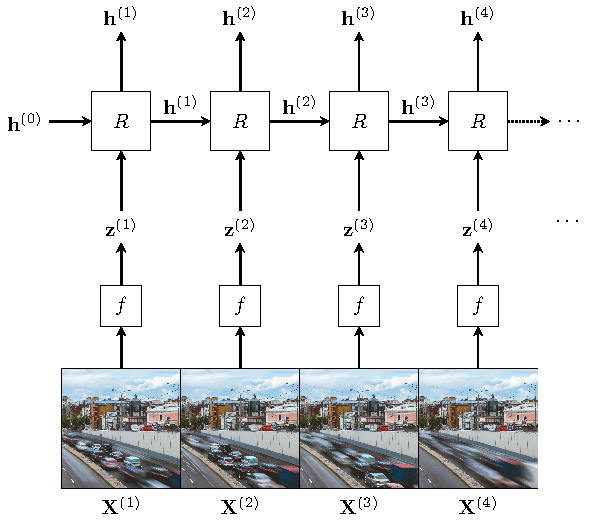
\includegraphics[width=\linewidth]{figures/normal_rnn.pdf}
    \caption{用 RNN 处理视频输入的示意图。每个输入视频帧 $\vec{X}^{(t)}$ 都由共享函数 $f$（例如平移不变 CNN）处理为扁平表示 $\vec{z}^{(t)}$。随后，RNN 更新函数 $R$ 在这些向量上迭代，不断更新概括向量 $\vec{h}^{(t)}$；该向量概括截至且包括 $\vec{z}^{(t)}$ 在内的所有输入。计算以初始概括向量 $\vec{h}^{(0)}$ 为起点，该向量可以预先确定，也可以学习。}
    \label{fig:normal_rnn}
\end{figure}
在每一步，循环神经网络都会计算一个 $m$ 维\emph{概括}向量 $\vec{h}^{(t)}$，用于概括截至且
包括 $t$ 在内的所有输入步骤。这一（部分）概括以当前步骤的
特征和前一步概括为条件，通过共享的\emph{更新}函数 $R : \mathbb{R}^k \times \mathbb{R}^m \rightarrow \mathbb{R}^m$ 按如下方式计算（概览见图 \ref{fig:normal_rnn}）：
\begin{equation}\label{eqn:rnn_upd}
    \vec{h}^{(t)} = R(\vec{z}^{(t)}, \vec{h}^{(t-1)})
\end{equation}
由于 $\vec{z}^{(t)}$ 和 $\vec{h}^{(t-1)}$ 都是\emph{扁平}向量表示，$R$ 最容易表示为单个全连接神经网络层（常称为 \emph{SimpleRNN}\marginnote{尽管名称如此，SimpleRNN 的表示能力非常强。例如，\citet{siegelmann1995computational} 证明这类模型是\emph{图灵完备的}，这意味着它们很可能可以表示我们能够在计算机上执行的\emph{任何}计算。}；见 \citet{elman1990finding,jordan1997serial}）：
\begin{equation}\label{eqn:SimpleRNN}
     \vec{h}^{(t)} = \sigma(\vec{W}\vec{z}^{(t)} + \vec{U}\vec{h}^{(t-1)} + \vec{b})
\end{equation}
其中 $\vec{W}\in\mathbb{R}^{k\times m}$、$\vec{U}\in\mathbb{R}^{m\times m}$ 和 $\vec{b}\in\mathbb{R}^m$ 是可学习参数，$\sigma$ 是激活函数。虽然这会在网络计算图中引入\emph{环}，但实践中
会把网络展开适当的步数，以便应用\emph{随时间反向传播} \citep{robinson1987utility,werbos1988generalization,mozer1989focused}。

随后可以为下游任务恰当利用这些概括向量：如果
需要在序列的每一步进行预测，可以对每个 $\vec{h}^{(t)}$ 分别应用共享预测器。若要对整个序列分类，通常把最终概括 $\vec{h}^{(T)}$ 传给分类器。这里，$T$ 是序列长度。

特别地，初始概括向量通常设为零向量，即 $\vec{h}^{(0)}=\vec{0}$，或者设为可学习。分析初始概括向量的设定方式，还可以推导出 RNN 所表现的一种有趣\emph{平移等变性}。

\paragraph{RNN 中的平移等变性}由于我们把各个步骤 $t$ 解释为\emph{离散时间步}，输入向量 $\vec{z}^{(t)}$ 可以看作位于一维时间步\marginnote{注意，该构造可以扩展到更高维网格，从而例如以\emph{扫描线}方式处理图像上的信号。该构造支撑了一系列流行模型，如 \citet{van2016pixel} 的 PixelRNN。}\emph{网格}上。虽然尝试把 CNN 的平移等变性分析扩展到这里很有吸引力，但不能直接做到这一点。

为说明原因，假设把序列向左平移一步，得到新序列 $\vec{z}'^{(t)} = \vec{z}^{(t+1)}$。%, recovering a new sequence $\vec{z}'^{(t)} = \vec{z}^{(t+1)}$.
按照平移等变性的预期，我们可能会尝试证明 $\vec{h}'^{(t)} = \vec{h}^{(t+1)}$，但这一般不成立。考虑 $t = 1$；直接应用并展开更新函数可得：
\begin{align}\label{eqn:shiftrnn}
    \vec{h}'^{(1)} &= R(\vec{z}'^{(1)}, \vec{h}^{(0)}) = R(\vec{z}^{(2)}, \vec{h}^{(0)})\\ 
    \vec{h}^{(2)} &= R(\vec{z}^{(2)}, \vec{h}^{(1)}) = R(\vec{z}^{(2)}, R(\vec{z}^{(1)}, \vec{h}^{(0)}))\label{eqn:shiftrnn2} 
\end{align}
因此，除非能保证 $\vec{h}^{(0)} = R(\vec{z}^{(1)}, \vec{h}^{(0)})$，否则无法得到平移等变性。随后可以对步骤 $t > 1$ 进行类似分析。

所幸，只需稍微调整 $\vec{z}$ 的表示方式并适当选择 $R$，就可以满足上述等式，从而给出 RNN 对平移等变的一种设定。
%
问题主要出在\emph{边界条件}：上述等式包含 $\vec{z}^{(1)}$，而左移操作破坏了它。为抽象掉这一问题，我们考察 RNN 如何处理经过适当\emph{左填充}的序列 $\bar{\vec{z}}^{(t)}$，其定义如下：
$$
    \bar{\vec{z}}^{(t)} = \begin{cases}
        \vec{0} & t \leq t'\\
        \vec{z}^{(t - t')} & t > t' 
    \end{cases}
$$
现在，这种序列允许最多左移\marginnote{注意，如果使用不同于 $\vec{0}$ 的填充向量，也会得到等价分析。}$t'$ 步，而不破坏任何原始输入元素。此外，无需单独处理右移；事实上，对右移的等变性自然可以从 RNN 方程推出。

现在可以再次分析 RNN 在 $\bar{\vec{z}}^{(t)}$ 左移版本上的运算，将其记为 $\bar{\vec{z}}'^{(t)} = \bar{\vec{z}}^{(t+1)}$，正如式 \ref{eqn:shiftrnn}--\ref{eqn:shiftrnn2} 中所做的那样：
\begin{align*}
    \vec{h}'^{(1)} &= R(\bar{\vec{z}}'^{(1)}, \vec{h}^{(0)}) = R(\bar{\vec{z}}^{(2)}, \vec{h}^{(0)})\\ \vec{h}^{(2)} &= R(\bar{\vec{z}}^{(2)}, \vec{h}^{(1)}) = R(\bar{\vec{z}}^{(2)}, R(\bar{\vec{z}}^{(1)}, \vec{h}^{(0)})) = R(\bar{\vec{z}}^{(2)}, R(\vec{0}, \vec{h}^{(0)}))
\end{align*}
替换 $\bar{\vec{z}}^{(1)} = \vec{0}$ 在 $t' \geq 1$ 时成立，即只要应用了任何填充便成立\marginnote{与此非常类似，可以推导出对左移 $s$ 步的等变性，只要 $t' \geq s$。}。现在，可以保证对左移一步的等变性（$\vec{h}'^{(t)} = \vec{h}^{(t+1)}$），只要 $\vec{h}^{(0)} = R(\vec{0}, \vec{h}^{(0)})$。


换言之，必须把 $\vec{h}^{(0)}$ 选为函数 $\gamma(\vec{h}) = R(\vec{0}, \vec{h})$ 的\emph{不动点}。如果恰当地选择更新函数 $R$，不仅可以保证这类不动点存在，甚至可以反复应用 $R$ 直至收敛，直接获得它们；例如：
\begin{equation}\label{eqn:iterated}
    \vec{h}_0 = \vec{0} \qquad \vec{h}_{k+1} = \gamma(\vec{h}_{k}),
\end{equation}
%
其中，索引 $k$ 表示计算中 $R$ 的迭代次数，与表示 RNN 时间步的索引 $(t)$ 相区别。
%
若选择 $R$ 使 $\gamma$ 成为\emph{压缩映射}\marginnote{压缩映射是如下函数 $\gamma: \mathcal{X}\rightarrow \mathcal{X}$：在某个范数 $\|\cdot\|$（定义于 $\mathcal{X}$ 上）下，应用 $\gamma$ 会\emph{压缩}点之间的距离；即对于所有 $\vec{x},\vec{y}\in\mathcal{X}$ 以及某个 $q\in [0,1)$，均有 $\|\gamma(\vec{x}) - \gamma(\vec{y})\| \leq q\|\vec{x} - \vec{y}\|$。反复迭代这类函数必然收敛到唯一不动点，这是 \emph{Banach 不动点定理} \citep{banach1922operations} 的直接推论。}，那么这种迭代确实会收敛到\emph{唯一}不动点。因此，可以迭代式~(\ref{eqn:iterated}) 直至 $\vec{h}_{k+1} = \vec{h}_k$，并令 $\vec{h}^{(0)} = \vec{h}_k$。注意，这一计算等价于用“足够多”的零向量对序列进行\emph{左填充}。

\paragraph{RNN 的深度}
堆叠多个 RNN 也很容易：只需把向量 $\vec{h}^{(t)}$ 作为第二个 RNN 的输入序列。这种构造有时称为“深层 RNN”，但这一名称可能产生误导。实际上，由于循环运算被反复应用，即便单个 RNN“层”的深度也\emph{等于输入步骤数}。

这通常会在优化 RNN 时引入格外棘手的学习动力学，因为每个训练样本都会对更新网络的\emph{共享}参数产生多次梯度更新。这里将关注其中或许最突出的问题——\emph{梯度消失}与\emph{梯度爆炸} \citep{bengio1994learning}。鉴于 RNN 的深度和参数共享，这一问题在 RNN 中尤其严重，并且单独推动了若干最有影响力的 RNN 研究。更详细的概述见 \citet{pascanu2013difficulty}；该工作深入研究了 RNN 的训练动力学，并从分析、几何和动力系统等多种视角揭示了这些挑战。

为说明梯度消失，考虑采用 S 形激活函数 $\sigma$ 的 SimpleRNN\marginnote{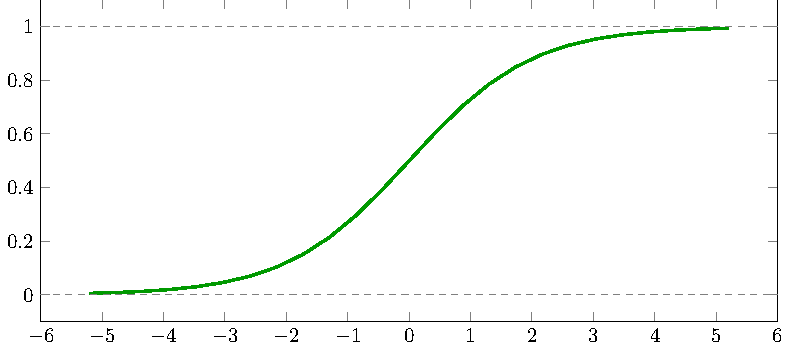
\includegraphics[width=\linewidth]{figures/sigmoid.pdf}\\ 这类激活函数包括\emph{logistic 函数} $\sigma(x) = \frac{1}{1+\exp(-x)}$ 和\emph{双曲正切} $\sigma(x)=\tanh x$。它们的图像具有鲜明的 S 形，因而称为 S 形函数。}，其导数绝对值 $|\sigma'|$ 始终介于 $0$ 与 $1$ 之间。许多个这样的值相乘，会使梯度迅速趋于零，这意味着输入序列中的早期步骤可能完全无法影响网络参数的更新。

例如，考虑下一词预测任务（常见于预测键盘等场景）和输入文本\emph{“Petar 是塞尔维亚人。他出生于 \dots [长段落] \dots Petar 目前居住在 \rule{1.3cm}{0.15mm}”}。这里，只有考虑段落最开头，才能合理推断下一个词是“塞尔维亚”；但梯度传播到这一输入步骤时很可能已经消失，使得从这类样本中学习非常困难。

深度前馈神经网络也曾受到梯度消失问题困扰，直到 ReLU 激活函数出现（其梯度\emph{恰好}等于零或一，因而解决了梯度消失问题）。然而，在 RNN 中使用 ReLU 很容易导致\emph{梯度爆炸}，因为更新函数的输出空间此时\emph{无界}，而梯度下降会为每个输入步骤更新一次单元，使更新量级迅速累积。
%
从历史上看，梯度消失现象很早就被视为使用循环网络的一项重大障碍。应对这一问题推动了更复杂 RNN 层的发展，下面将对其进行介绍。


\subsection{长短期记忆网络}
\label{sec:lstm}

\begin{figure}
    \centering
    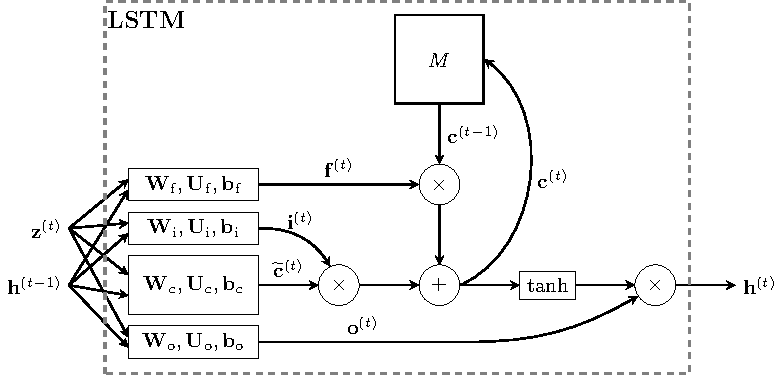
\includegraphics[width=\linewidth]{figures/lstm.pdf}
    \caption{长短期记忆（LSTM）的数据流，其中各组成部分和记忆单元（$M$）均清晰标出。根据当前输入 $\vec{z}^{(t)}$、前一概括 $\vec{h}^{(t-1)}$ 和前一单元状态 $\vec{c}^{(t-1)}$，LSTM 预测更新后的单元状态 $\vec{c}^{(t)}$ 和概括 $\vec{h}^{(t)}$。}
    \label{fig:lstm}
\end{figure}
显著减轻 RNN 中梯度消失影响的一项关键发明是\emph{门控机制}，它允许网络以数据驱动方式选择性地\emph{覆写}信息。这类\emph{门控 RNN} 的著名实例包括{\em 长短期记忆}（LSTM；\citet{hochreiter1997long}）和{\em 门控循环单元}（GRU；\citet{cho2014learning}）。为说明此类模型的运算，这里主要讨论 LSTM，具体采用 \citet{graves2013generating} 提出的变体。LSTM 中的概念很容易推广到其他门控 RNN。

阅读本节时，参照图 \ref{fig:lstm} 可能会有所帮助；该图展示了正文将讨论的全部 LSTM 运算。

LSTM 通过引入\emph{记忆单元}来扩展循环计算；该单元存储在计算步骤之间得到\emph{保留}的\emph{单元状态}向量 $\vec{c}^{(t)}\in\mathbb{R}^m$。LSTM 计算概括向量 $\vec{h}^{(t)}$，直接以 $\vec{c}^{(t)}$ 为依据，而 $\vec{c}^{(t)}$ 又使用 $\vec{z}^{(t)}$、$\vec{h}^{(t-1)}$ 和 $\vec{c}^{(t-1)}$ 计算。
关键在于，单元\textbf{不会}根据 $\vec{z}^{(t)}$ 和 $\vec{h}^{(t-1)}$ 被完全覆写，否则网络将面临与 SimpleRNN 相同的问题。相反，可以\emph{保留}一定比例的前一单元状态，而这一比例由数据显式\emph{学习}得到。

与 SimpleRNN 一样，我们在当前输入步骤和前一概括上使用单个全连接神经网络层计算特征：\marginnote{注意，这里把激活函数设为 $\tanh$；由于 LSTM 旨在缓解梯度消失问题，此时使用 S 形激活函数是合适的。}
\begin{equation}\label{eqn:lstmstart}
     \widetilde{\vec{c}}^{(t)} = \tanh(\vec{W}_c\vec{z}^{(t)} + \vec{U}_c\vec{h}^{(t-1)} + \vec{b}_c)
\end{equation}
但是，如前所述，我们不允许该向量的\emph{全部}分量进入单元，因此称它为\emph{候选}特征向量，并记为 $\widetilde{\vec{c}}^{(t)}$。LSTM 转而直接学习\emph{门控向量}；它们是范围 $[0, 1]$ 内的实值向量，用于决定允许多少信号进入、离开和覆写记忆单元。

一共计算三个这样的门，它们都基于 $\vec{z}^{(t)}$ 和 $\vec{h}^{(t-1)}$：\emph{输入门} $\vec{i}^{(t)}$ 计算允许进入单元的候选向量比例；\emph{遗忘门} $\vec{f}^{(t)}$ 计算要保留的前一单元状态比例；\emph{输出门} $\vec{o}^{(t)}$ 计算用于最终概括向量的新单元状态比例。通常，所有这些门也通过单个全连接层得到，但使用\emph{logistic sigmoid} 激活 $\mathrm{logistic}(x) = \frac{1}{1+\exp(-x)}$，以保证输出位于 $[0, 1]$ 范围内\marginnote{注意，这三个门本身是\emph{向量}，即 $\vec{i}^{(t)}, \vec{f}^{(t)}, \vec{o}^{(t)}\in [0,1]^m$。这使它们能够控制 $m$ 个维度中的\emph{每一个}有多少分量可通过门。}：
\begin{align}\label{eqn:lstm_gate}
     \vec{i}^{(t)} &= \mathrm{logistic}(\vec{W}_\mathrm{i}\vec{z}^{(t)} + \vec{U}_\mathrm{i}\vec{h}^{(t-1)} + \vec{b}_\mathrm{i})\\
     \vec{f}^{(t)} &= \mathrm{logistic}(\vec{W}_\mathrm{f}\vec{z}^{(t)} + \vec{U}_\mathrm{f}\vec{h}^{(t-1)} + \vec{b}_\mathrm{f})\\
     \vec{o}^{(t)} &= \mathrm{logistic}(\vec{W}_\mathrm{o}\vec{z}^{(t)} + \vec{U}_\mathrm{o}\vec{h}^{(t-1)} + \vec{b}_\mathrm{o})
\end{align}

最后，恰当地应用这些门以解码\emph{新的}单元状态 $\vec{c}^{(t)}$，再由输出门对其调制以产生概括向量 $\vec{h}^{(t)}$，如下所示：
\begin{align}
    \vec{c}^{(t)} &= \vec{i}^{(t)}\odot\widetilde{\vec{c}}^{(t)} + \vec{f}^{(t)}\odot\vec{c}^{(t-1)}\\
    \vec{h}^{(t)} &= \vec{o}^{(t)}\odot\tanh(\vec{c}^{(t)})\label{eqn:lstm_end}
\end{align}
其中 $\odot$ 表示向量逐元素乘法。式 (\ref{eqn:lstmstart})--(\ref{eqn:lstm_end}) 共同完整指定了 LSTM 的\emph{更新规则}，该规则现在还考虑单元向量 $\vec{c}^{(t)}$\marginnote{这仍与式 (\ref{eqn:rnn_upd}) 的 RNN 更新蓝图兼容；只需把概括向量视为 $\vec{h}^{(t)}$ 和 $\vec{c}^{(t)}$ 的\emph{拼接}，有时记为 $\vec{h}^{(t)}\|\vec{c}^{(t)}$。}：
$$
    (\vec{h}^{(t)}, \vec{c}^{(t)}) = R(\vec{z}^{(t)}, (\vec{h}^{(t-1)}, \vec{c}^{(t-1)}))
$$
注意，由于 $\vec{f}^{(t)}$ 的值由 $\vec{z}^{(t)}$ 和 $\vec{h}^{(t-1)}$ 得到，因而可直接从数据中\emph{学习}，LSTM 实际上学会了如何恰当地遗忘过去的经验。事实上，$\vec{f}^{(t)}$ 的值直接出现在所有 LSTM 参数（$\vec{W}_*, \vec{U}_*, \vec{b}_*$）的反向传播更新中，使网络能够以数据驱动方式显式\emph{控制}梯度跨时间步消失的程度。

除了直接应对梯度消失问题外，门控 RNN 还带来一种非常有用的对\emph{时间扭曲}变换的不变性，而 SimpleRNN 无法获得这种性质。

\paragraph{门控 RNN 的时间扭曲不变性}我们首先在\emph{连续时间}设定下说明\marginnote{之所以关注连续设定，是因为在其中更容易对时间操作进行推理。}\emph{扭曲时间}意味着什么，以及循环模型要对这类变换实现不变性需要满足哪些条件。我们的论述主要遵循 \citet{tallec2018can} 的工作；该工作最初描述了这一现象，而且确实是最早从不变性视角研究 RNN 的工作之一。

假设有一个连续时域信号 $z(t)$，我们希望在其上应用 RNN。为使 RNN 对概括向量 $\vec{h}^{(t)}$ 的离散时间计算\marginnote{我们用 $h(t)$ 表示时间 $t$ 的连续信号，用 $\vec{h}^{(t)}$ 表示时间步 $t$ 的离散信号。}与连续域中的对应量 $h(t)$ 对齐，考察其线性 Taylor 展开：
\begin{equation}
    h(t + \delta) \approx h(t) + \delta\frac{\mathrm{d}h(t)}{\mathrm{d}t}
\end{equation}
令 $\delta = 1$，便可恢复 $h(t)$ 与 $h(t+1)$ 之间的关系，这正是 RNN 更新函数 $R$（式 \ref{eqn:rnn_upd}）所计算的内容。具体而言，RNN 更新函数满足下列微分方程：
\begin{equation}\label{eqn:ode_pre_warp}
    \frac{\mathrm{d}h(t)}{\mathrm{d}t} = h(t+1) - h(t) = R(z(t+1), h(t)) - h(t)
\end{equation}

我们希望 RNN 对信号的采样方式（例如改变时间计量单位）具有稳健性，以适应其中的任何缺陷或不规则性。形式上，我们把\emph{时间扭曲}\marginnote{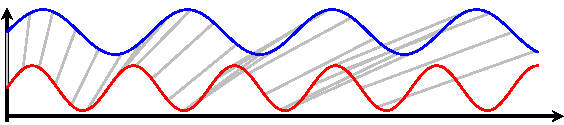
\includegraphics[width=\linewidth]{figures/time_warp.pdf}\\ 这类扭曲运算可以很\emph{简单}，例如时间重缩放；如上图所示的 $\tau(t) = 0.7t$，在离散设定下相当于每隔 $\sim 1.43$ 步接收一个新输入。不过，它也允许各种\emph{可变}采样率，例如采样可以在整个时域中自由加速或减速。}运算 $\tau : \mathbb{R}^+\rightarrow\mathbb{R}^+$ 定义为时间之间任意单调递增的可微映射。之所以选择记号 $\tau$，是因为时间扭曲表示时间的一个\emph{自同构}。

进一步地，如果对于该类中的任意模型和任意这样的 $\tau$，都存在该类中的另一个模型（可能是同一个模型），能够以原模型处理未扭曲数据的相同方式处理扭曲后的数据，我们就称这一模型类对时间扭曲\emph{不变}。

这是一项可能非常有用的性质。如果某个 RNN 类能够很好地建模短期依赖，并且可以证明该类对时间扭曲不变，那么就知道可以通过训练使这类模型也有效捕获长期依赖（因为长期依赖对应于对具有短期依赖的信号进行时间膨胀扭曲）。
%
下文很快会看到，LSTM 等\emph{门控} RNN 模型被提出用于建模长程依赖并非巧合。实现时间扭曲不变性与门控机制的存在紧密相关，例如 LSTM 的输入门、遗忘门和输出门。

当时间由 $\tau$ 扭曲时，RNN 在时间 $t$ 观察到的信号是 $z(\tau(t))$；为了对这类扭曲保持不变，它应预测经过等价扭曲的概括函数 $h(\tau(t))$。再次使用 Taylor 展开，可以推导出式 \ref{eqn:ode_pre_warp} 在扭曲时间下的形式，RNN 更新 $R$ 应满足该形式：
\begin{equation}\label{eqn:ode_post_warp}
    \frac{\mathrm{d}h(\tau(t))}{\mathrm{d}\tau(t)} = R(z(\tau(t+1)), h(\tau(t))) - h(\tau(t))
\end{equation}
然而，上述导数是相对于扭曲时间 $\tau(t)$ 计算的，因此没有考虑原始信号。为使模型显式考虑扭曲变换，需要相对于 $t$ 对扭曲后的概括函数求导。应用链式法则得到下列微分方程：
\begin{equation}\label{eqn:full_ode_warp}
    \frac{\mathrm{d}h(\tau(t))}{\mathrm{d}t} = \frac{\mathrm{d}h(\tau(t))}{\mathrm{d}\tau(t)}\frac{\mathrm{d}\tau(t)}{\mathrm{d}t} = \frac{\mathrm{d}\tau(t)}{\mathrm{d}t}R(z(\tau(t+1)), h(\tau(t))) - \frac{\mathrm{d}\tau(t)}{\mathrm{d}t}h(\tau(t))
\end{equation}
而且，为使（连续时间）RNN 对\emph{任意}时间扭曲 $\tau(t)$ 保持不变，它必须能够显式表示导数 $\frac{\mathrm{d}\tau(t)}{\mathrm{d}t}$，但我们并不假设事先知道该导数！因此需要引入一个近似此导数的\emph{可学习}函数 $\Gamma$。例如，$\Gamma$ 可以是考虑 $z(t+1)$ 和 $h(t)$ 并预测标量输出的神经网络。

现在注意，从时间扭曲下的\emph{离散} RNN 模型视角看，其输入 $\vec{z}^{(t)}$ 对应于 $z(\tau(t))$，其概括 $\vec{h}^{(t)}$ 对应于 $h(\tau(t))$。为获得 $\vec{h}^{(t)}$ 与 $\vec{h}^{(t+1)}$ 之间保持时间扭曲不变性所需的关系，我们对 $h(\tau(t))$ 进行一步 Taylor 展开：
\begin{equation*}
    h(\tau(t + \delta)) \approx h(\tau(t)) + \delta\frac{\mathrm{d}h(\tau(t))}{\mathrm{d}t}
\end{equation*}
再次令 $\delta=1$，代入式 \ref{eqn:full_ode_warp}，然后离散化：
\begin{align*}
    \vec{h}^{(t+1)} &= \vec{h}^{(t)} + \frac{\mathrm{d}\tau(t)}{\mathrm{d}t}R(\vec{z}^{(t+1)}, \vec{h}^{(t)}) - \frac{\mathrm{d}\tau(t)}{\mathrm{d}t}\vec{h}^{(t)}\\
    &= \frac{\mathrm{d}\tau(t)}{\mathrm{d}t}R(\vec{z}^{(t+1)}, \vec{h}^{(t)}) + \left(1 - \frac{\mathrm{d}\tau(t)}{\mathrm{d}t}\right)\vec{h}^{(t)}
\end{align*}
最后，把 $\frac{\mathrm{d}\tau(t)}{\mathrm{d}t}$ 替换为前述可学习函数 $\Gamma$。由此得到时间扭曲不变 RNN 所需的形式：
\begin{equation}\label{eqn:GaRNN}
    \vec{h}^{(t+1)} = \Gamma(\vec{z}^{(t+1)}, \vec{h}^{(t)})R(\vec{z}^{(t+1)}, \vec{h}^{(t)}) + (1 - \Gamma(\vec{z}^{(t+1)}, \vec{h}^{(t)}))\vec{h}^{(t)}
\end{equation}
可以很快推断，SimpleRNN（式 \ref{eqn:SimpleRNN}）\emph{不}具有时间扭曲不变性，因为它们不包含式 \ref{eqn:GaRNN} 中的第二项。相反，$\vec{h}^{(t)}$ 被 $R(\vec{z}^{(t+1)}, \vec{h}^{(t)})$ 完全覆写，这对应于假设根本没有时间扭曲，即 $\frac{\mathrm{d}\tau(t)}{\mathrm{d}t} = 1$，也就是 $\tau(t) = t$。

此外，连续时间 RNN 与基于 $R$ 的离散 RNN 之间的联系依赖于 Taylor 近似的准确性，而只有时间扭曲导数不太大时该近似才成立，即 $\frac{\mathrm{d}\tau(t)}{\mathrm{d}t}\lesssim 1$。直观解释如下：如果时间扭曲运算以某种方式\emph{压缩时间}，使时间增量（$t \rightarrow t + 1$）大到无法采样中间的数据变化，那么模型永远不可能以处理原始输入的相同方式处理时间扭曲输入，因为它根本无法获得相同信息。相反，我们的框架完全允许任何形式的时间\emph{膨胀}（在离散意义下，这对应于在输入时间序列中插入零）。

结合 $\tau$ 单调递增这一要求（$\frac{\mathrm{d}\tau(t)}{\mathrm{d}t} > 0$），可以把 $\Gamma$ 的输出空间限制为 $0 < \Gamma(\vec{z}^{(t+1)}, \vec{h}^{(t)}) < 1$，这促使我们为 $\Gamma$ 使用 logistic sigmoid 激活，例如：
$$
    \Gamma(\vec{z}^{(t+1)}, \vec{h}^{(t)}) = \mathrm{logistic}({\bf W}_\Gamma\vec{z}^{(t+1)} + {\bf U}_\Gamma\vec{h}^{(t)} + \vec{b}_\Gamma)
$$
这与 LSTM 门控方程\emph{完全}一致（例如式 \ref{eqn:lstm_gate}）。主要区别在于，LSTM 计算门控\emph{向量}，而式 \ref{eqn:GaRNN} 意味着 $\Gamma$ 应输出标量。向量化门 \citep{hochreiter1991untersuchungen} 允许在 $\vec{h}^{(t)}$ 的每个维度拟合\emph{不同的}扭曲导数，从而同时对\emph{多个}时间跨度进行推理。

这里有必要稍作停顿，总结已经完成的工作。通过要求 RNN 类对（非破坏性）时间扭曲不变，我们推导出它必须具有的必要形式（式 \ref{eqn:GaRNN}），并证明该形式恰好对应于\emph{门控} RNN 类。在这一视角下，门的主要作用是准确拟合扭曲变换的\emph{导数} $\frac{\mathrm{d}\tau(t)}{\mathrm{d}t}$。

\emph{类不变性}的概念与此前研究的不变性有所不同。也就是说，一旦在采用 $\tau_1(t)$ 时间扭曲的输入上训练了门控 RNN，通常不能将其零样本迁移\marginnote{可以进行零样本迁移的一种情形是，假设第二次时间扭曲是第一次的\emph{时间重缩放}（$\tau_2(t) = \alpha\tau_1(t)$）。把在 $\tau_1$ 上预训练的门控 RNN 迁移到由 $\tau_2$ 扭曲的信号，只需\emph{重缩放门}：$\Gamma_2(\vec{z}^{(t+1)}, \vec{h}^{(t)}) = \alpha \Gamma_1(\vec{z}^{(t+1)}, \vec{h}^{(t)})$。$R$ 可以保留其参数（$R_1 = R_2$）。}到由不同 $\tau_2(t)$ 扭曲的信号。相反，类不变性只保证门控 RNN 具有足够的表达能力，能以相同方式拟合这两个信号，但其模型参数可能大不相同。尽管如此，有效门控机制与拟合扭曲导数紧密相关这一认识，可以为门控 RNN 优化提供有用准则，下面作简要说明。

例如，通常可以假设，我们希望在信号中跟踪的依赖关系跨度位于 $[T_l, T_h]$ 个时间步的范围内。

通过分析式 \ref{eqn:full_ode_warp} 的解析解，可以证明，门控 RNN 对 $\vec{h}^{(t)}$ 的特征\emph{遗忘时间}与 $\frac{1}{\Gamma(\vec{z}^{(t+1)}, \vec{h}^{(t)})}$ 成正比。因此，为了有效记住假设范围内的信息，我们希望门控值位于 $\left[\frac{1}{T_h}, \frac{1}{T_m}\right]$ 之间。

进一步地，若假设 $\vec{z}^{(t)}$ 和 $\vec{h}^{(t)}$ 大致\emph{以零为中心}——这是应用层归一化 \citep{ba2016layer} 等变换时常见的副产物——则可以假设 $\mathbb{E}[\Gamma(\vec{z}^{(t+1)}, \vec{h}^{(t)})] \approx \mathrm{logistic}(\vec{b}_\Gamma)$。因此，控制门控机制的\emph{偏置}向量是控制有效门值的一种非常有力的方法\marginnote{\citet{gers2000recurrent,jozefowicz2015empirical} 已经发现这一洞见，并根据经验建议把 LSTM 的遗忘门偏置初始化为常数正向量，例如 $\vec{1}$。}。

结合上述两个观察，可以得出结论：通过初始化 $\vec{b}_\Gamma\sim-\log(\mathcal{U}(T_l, T_h) - 1)$ 可以获得合适范围的门控值，其中 $\mathcal{U}$ 是实数均匀分布。\citet{tallec2018can} 将这一建议称为\emph{时间尺度初始化}，经验证明它可以改善门控 RNN 对长程依赖的建模。

\paragraph{使用 RNN 的序列到序列学习}
使用 RNN 支撑计算的一个著名历史实例是\emph{序列到序列}翻译任务，例如自然语言的{\em 机器翻译}。\citet{sutskever2014sequence} 开创性的 \emph{seq2seq} 工作把概括向量 $\vec{h}^{(T)}$ 作为\emph{解码器} RNN 的初始输入，并把 RNN 模块的输出作为下一步输入，从而实现了这一目标。

\begin{figure}
    \centering
    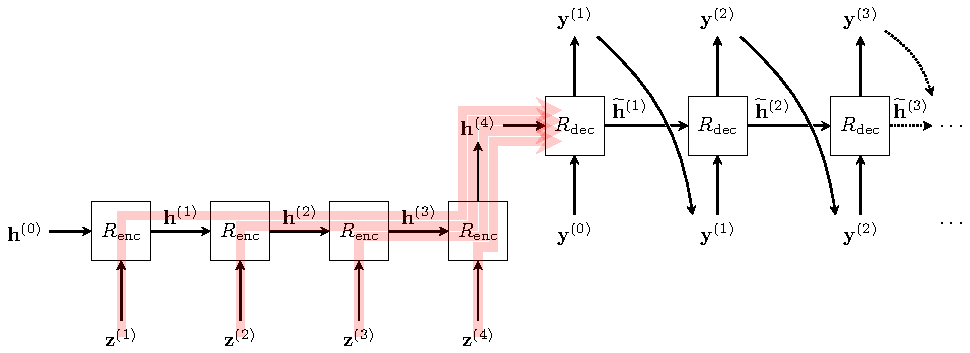
\includegraphics[width=\linewidth]{figures/bottle_rnn.pdf}
    \caption{seq2seq 架构的一个典型实例，包含 RNN 编码器 $R_\mathrm{enc}$ 和 RNN 解码器 $R_\mathrm{dec}$。解码器以编码器输出的最终概括向量 $\vec{h}^{(T)}$ 为初始状态，然后以\emph{自回归}方式运行：在每一步，前一步的预测输出都作为输入反馈给 $R_\mathrm{dec}$。红线还示意了瓶颈问题：概括向量 $\vec{h}^{(T)}$ 被迫存储翻译输入序列所需的\emph{全部}相关信息，随着输入长度增加，这一点会越来越困难。}
    \label{fig:rnn_bottleneck}
\end{figure}

这给概括向量 $\vec{h}^{(T)}$ 带来了巨大的表示压力。在深度学习语境下，$\vec{h}^{(T)}$ 有时称为\emph{瓶颈}\marginnote{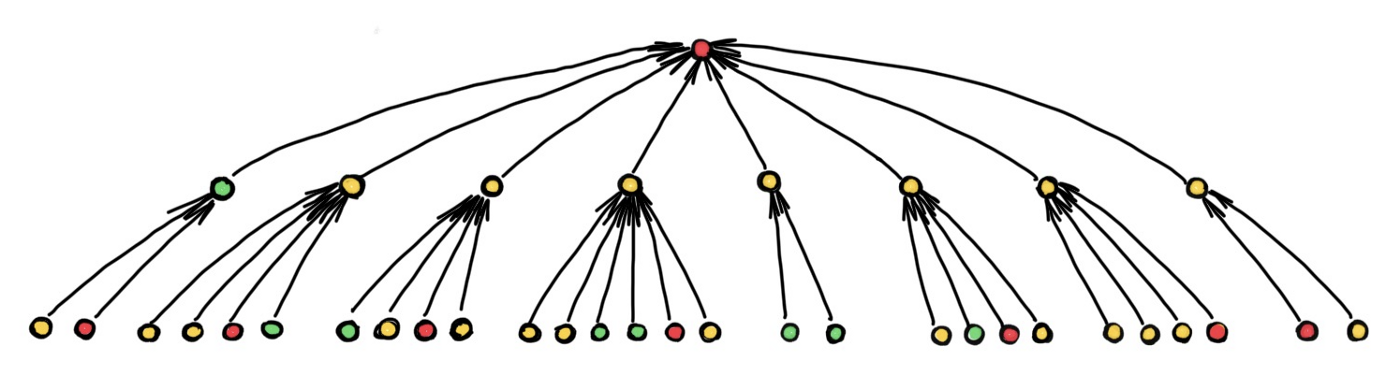
\includegraphics[width=\linewidth]{figures/bottleneck.png}\\
瓶颈效应最近在图表示学习社群 \citep{alon2020bottleneck} 以及神经算法推理领域 \citep{cappart2021combinatorial} 受到广泛关注。}。它的固定容量必须足以表示整个输入序列的内容，其表示方式还要有利于生成相应序列，同时支持长度相差很大的输入序列（图 \ref{fig:rnn_bottleneck}）。

实际上，输出的不同步骤可能希望聚焦（\emph{关注}）输入的不同部分，而所有这些选择都难以通过瓶颈向量表示。基于这一观察，\citet{bahdanau2014neural} 提出了流行的\emph{循环注意力}模型。在处理的每一步，RNN 都会生成一个\emph{查询向量}；该查询向量随后与\emph{每个}时间步的表示 $\vec{h}^{(t)}$ 交互，主要方式是对它们计算加权和。该模型开创了神经内容注意力，并早于 Transformer 模型的成功。

最后，虽然注意力提供了一种动态聚焦输入内容各部分的\emph{软}方式，大量工作也学习了以更\emph{显式}的方式把注意力指向输入。\citet{vinyals2015pointer} 的\emph{指针网络}是一种具有算法依据的有力方法：它对循环注意力作简单修改，从而允许指向\emph{大小可变}输入中的元素。随后，这些结论被推广到 \emph{set2set} 架构 \citep{vinyals2016order}；该架构借助由指针网络支撑的 LSTM，把 seq2seq 模型推广到无序集合。




\section{问题与应用}

不变性与对称性在源自现实世界的数据中极为常见。因此，21 世纪一些最流行的机器学习应用直接源于几何深度学习并不令人意外，尽管人们有时可能并未充分意识到这一点。
%
我们希望为读者概述几何深度学习中具有影响力的工作以及令人振奋且前景可期的新应用，但这份概述绝非面面俱到。这样做有两个目的：一是展示五类几何域经常出现于哪些具体的科学与工业问题中，二是进一步说明研究几何深度学习原理与架构的必要性。



\paragraph{化学与药物设计} 图上表示学习最具前景的应用之一，是计算化学和\emph{药物开发}。\marginnote{许多药物并非经由设计而得，而是被发现的，且往往出于偶然。多种药物在历史上源自植物界，这一点也反映在它们的名称中。例如，%ephedrine takes its name from the plant genus {\em Ephedra}, atropine from the belladonna plant ({\em Atropa belladonna}), and
通常称为\emph{阿司匹林}的乙酰水杨酸存在于白柳（\emph{Salix alba}）树皮中，而其药用性质自古便为人所知。
} 
%
传统药物是经过设计的小分子，
旨在以化学方式附着（“结合”）到某个靶分子（通常是蛋白质）上，从而激活或阻断某种与疾病相关的化学过程。
%
遗憾的是，药物开发是一个极其漫长且昂贵的过程：
在本文写作之时，
一种新药上市通常需要十年以上，耗资超过十亿美元。
%
原因之一是测试成本；
许多药物会在不同阶段失败——能够进入最后阶段的候选药物不足 5\%（例如见 \cite{gaudelet2020utilising}）。




由于化学上可合成分子的空间极其庞大（估计约为 $10^{60}$），无法通过实验搜索同时具备适当靶标结合亲和力、低毒性、溶解性等性质的候选分子，因而需要采用\emph{虚拟筛选}或\emph{计算机模拟筛选}（即用计算技术识别有前景的分子）。机器学习技术在这项任务中发挥着日益重要的作用。
%
%
\citet{stokes2020deep} 最近给出了几何深度学习用于虚拟药物筛选的一个突出实例：%have definitively demonstrated that this is possible:
他们训练图神经网络预测候选分子能否抑制模式细菌 \emph{Escherichia coli} 的生长，\marginnote{ 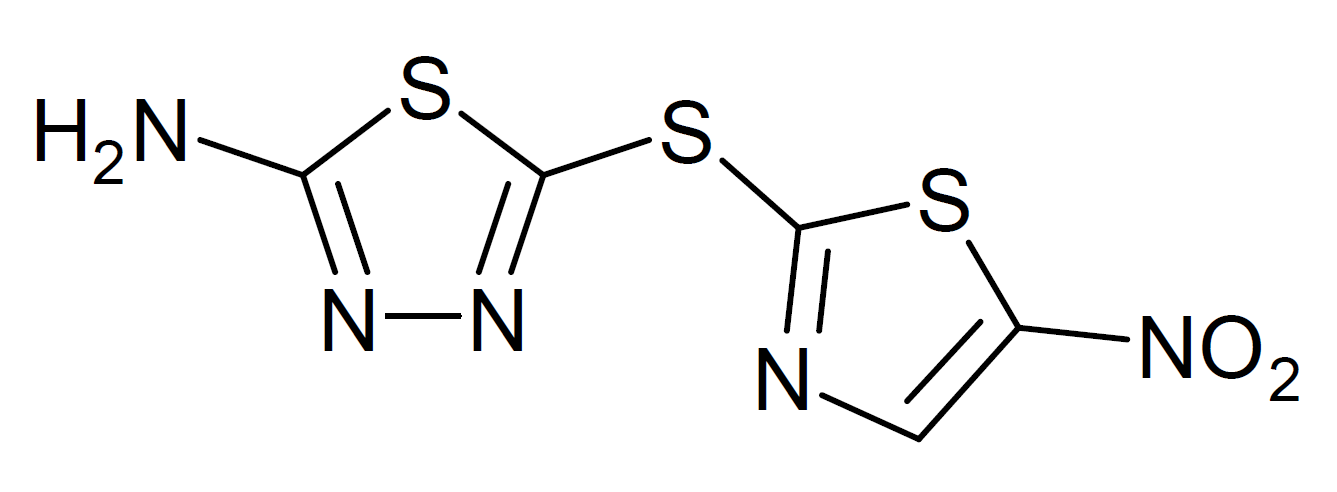
\includegraphics[width=\linewidth]{figures/Halicin_structure.png}\\ Halicin 的分子图。}并由此有效发现，原本适用于治疗糖尿病的分子 \emph{Halicin} 是一种强效抗生素，甚至能够对抗已知具有抗生素耐药性的细菌菌株。这一发现得到了科学媒体和大众媒体的广泛报道。


更广泛地说，把图神经网络应用于建模为图的分子一直是一个非常活跃的领域。近期提出的多种专门架构受到物理学启发，例如纳入了对旋转和平移的等变性（例如见 \cite{thomas2018tensor,anderson2019cormorant,fuchs2020se,satorras2021n}）。此外，\citet{bapst2020unveiling} 成功证明了 GNN 在玻璃动力学预测建模中的效用，其性能超过了此前已有的物理模型。
%
从历史上看，计算化学中的许多工作都是现代图神经网络架构的先驱，并与后者具有许多共同特征。




\paragraph{药物再定位}
%
%\marginnote}---being able to detect novel therapeutics for existing or emerging diseases---commonly by analysing the candidate drug's molecular graph. 
尽管生成全新的候选药物可能是一条可行路径，但开发新疗法还有一种更快、更经济的途径，即\emph{药物再定位}：评估已获批准的药物（单独使用或联合使用）能否用于新的目的。
%
这通常能显著减少药物上市所必需的临床评估。%
在某种抽象层次上，药物对人体生物化学过程的作用，以及药物彼此之间和与其他生物分子的相互作用，都可以建模为图。由此产生了著名网络科学家 Albert-L{\'a}szl{\'o} Barab{\'a}si 提出的“网络医学”概念；该概念主张利用生物网络（如蛋白质--蛋白质相互作用网络和代谢通路）开发新疗法 \citep{barabasi2011network}。


几何深度学习为这类方法提供了现代化视角。一个突出的早期实例是 \cite{zitnik2018modeling} 的工作：他们使用图神经网络预测一种称为\emph{组合疗法}或\emph{多重用药}的药物再定位方案所产生的副作用，并把该问题表述为药物--药物相互作用图中的边预测。
%
在本文写作时仍大范围持续的新型冠状病毒疫情，使人们对以下方向产生了特别浓厚的兴趣：%detecting novel therapeutics; see, e.g.,
尝试应用这类方法对抗 COVID-19 \citep{gysi2020network}。
%
最后需要指出，药物再定位未必局限于合成分子：\cite{veselkov2019hyperfoods} 把类似方法用于食物中所含的类药分子（正如前面提到的，许多植物性食物含有肿瘤治疗所用化合物的生物类似物）。
%
本文的一位作者参与了一项为该研究增添创意的合作：与一位分子料理厨师合作，利用富含这类类药分子的“超级食物”食材设计令人兴奋的菜谱。


\paragraph{蛋白质生物学}
既然已经提到作为药物靶标的蛋白质，我们不妨再花一些篇幅讨论这一主题。
%
蛋白质可以说是最重要的一类生物分子，
%often called the ``molecules of life'', as we are currently not aware of any life-form that is not protein-based. Proteins are encoded in our DNA and 
在人体内承担着无数功能，包括抵御病原体（抗体）、赋予皮肤结构（胶原蛋白）、向细胞输送氧气（血红蛋白）、催化化学反应（酶）以及传递信号（许多激素都是蛋白质）。
%
从化学角度看，蛋白质是一种生物聚合物，即由称为\emph{氨基酸}的小型构件组成的链；它在静电力作用下折叠成复杂的 3D 结构。正是这种结构赋予了蛋白质功能，\marginnote{一个常见比喻可追溯到化学诺贝尔奖得主 Emil Fischer 提出的\emph{Schl{\"u}ssel-Schloss-Prinzip}（“钥匙--锁原理”，1894 年）：两个蛋白质往往只有在几何结构和化学结构互补时才会相互作用。}因此，它对于理解蛋白质如何工作及其功能至关重要。由于蛋白质是药物治疗的常见靶标，%(typical drugs are small molecules designed to bind to their target),
制药行业对这一领域抱有浓厚兴趣。

%\michael{Put AlphaFold here? }

蛋白质生物信息学中的典型问题层次，是从蛋白质\emph{序列}（由 20 种不同氨基酸构成字母表上的 1D 字符串），到 3D \emph{结构}（称为“蛋白质折叠”的问题），再到\emph{功能}（“蛋白质功能预测”）。
%
近期方法（例如 \cite{senior2020improved} 提出的 DeepMind AlphaFold）使用\emph{接触图}表示蛋白质结构。\cite{gligorijevic2020structure} 表明，在这类图上应用图神经网络，能够取得优于纯序列方法的功能预测结果。


\cite{gainza2020deciphering} 开发了名为 MaSIF 的几何深度学习流水线，\marginnote{ 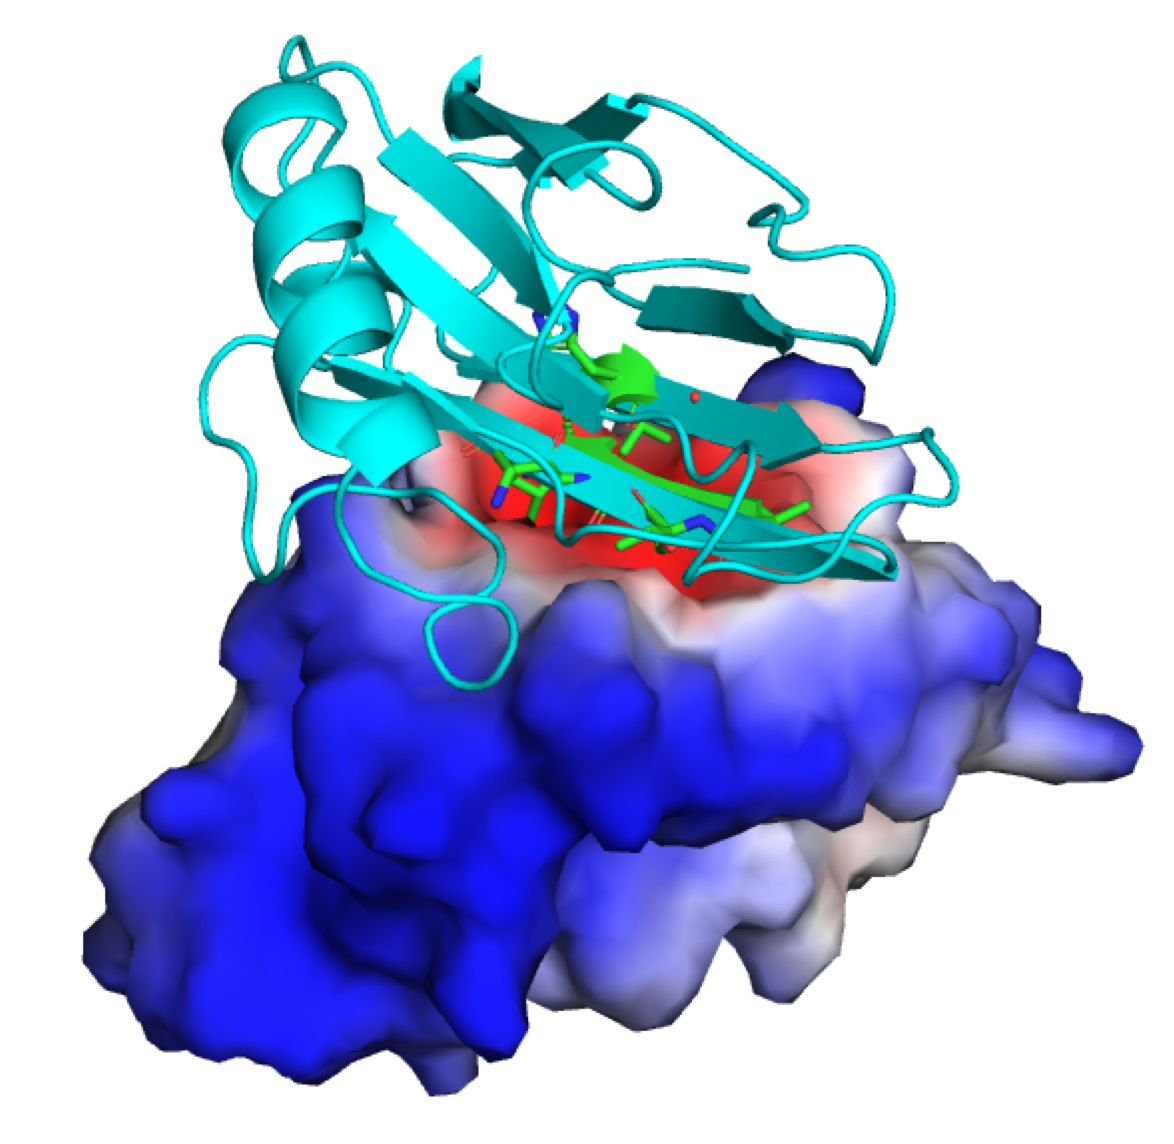
\includegraphics[width=\linewidth]{figures/masif.png}\\ 肿瘤靶标 PD-L1 的蛋白质表面（热图表示预测的结合位点）以及设计得到的结合体（以带状图显示）。}根据蛋白质的 3D 结构预测蛋白质间相互作用。MaSIF 把蛋白质建模为离散成网格曲面的分子表面，并指出这种表示在处理相互作用时具有优势，因为它能够抽象掉内部折叠结构。该架构基于网格曲面卷积神经网络，对小型局部测地线斑块中预先计算的化学与几何特征进行运算。%
该网络使用 Protein Data Bank 中数千个蛋白质共晶 3D 结构进行训练，以处理界面预测、配体分类和对接等多项任务；它还能够\emph{从头}设计理论上可作为抗癌生物免疫治疗药物的蛋白质。这类蛋白质旨在抑制程序性细胞死亡蛋白复合物各部分（PD-1/PD-L1）之间的蛋白质--蛋白质相互作用（PPI），使免疫系统获得攻击肿瘤细胞的能力。%showing state-of-the-art performance.

%A key difference of MaSIF compared to other methods is that it does not rely on the evolutionary history of proteins. This is of crucial importance in de novo protein design, where one tries to create “from scratch” new proteins that have never existed before.



\paragraph{推荐系统与社交网络} 图表示学习最早得到普及的大规模应用出现在\emph{社交网络}\marginnote{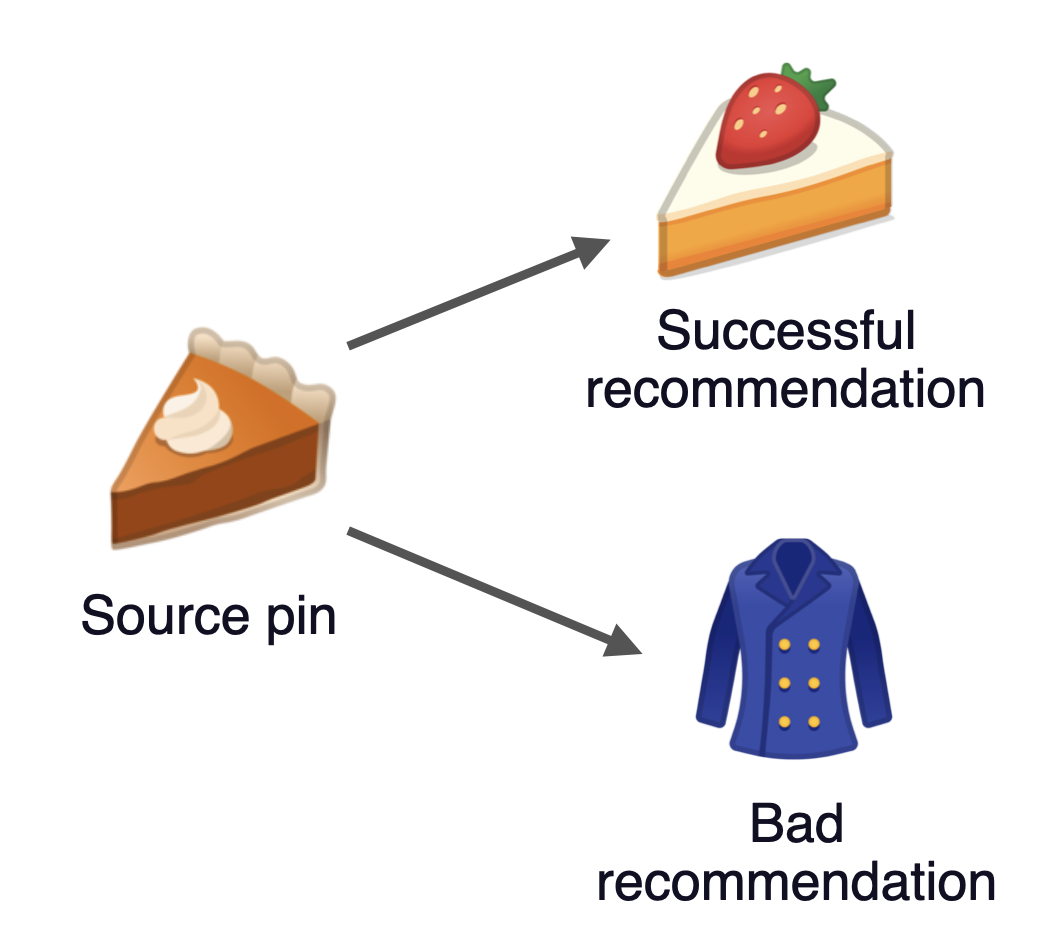
\includegraphics[width=\linewidth]{figures/Recommender.png}}中，主要应用场景是\emph{推荐系统}。推荐器的任务是决定向用户提供哪些内容，这一决定可能取决于用户此前在服务中的交互历史。该任务通常通过\emph{链接预测}目标实现：对各种节点（内容项）的嵌入进行监督，使被认为\emph{相关}的节点（例如经常被共同浏览的内容）彼此接近。于是，两个嵌入的\emph{接近程度}（例如它们的内积）可以解释为二者在内容图中由一条边连接的概率；因此，对于用户查询的任意内容，一种做法是在嵌入空间中提供其 $k$ 个最近邻。

这一方法的先驱之一是美国图片分享与社交媒体公司 Pinterest：除了率先成功地在生产环境中部署 GNN 之外，其 PinSage 方法\marginnote{Pinterest 还提出了后续工作 PinnerSage \citep{pal2020pinnersage}，它把用户特定的上下文信息有效整合进推荐器。}还成功使图表示学习能够\emph{扩展}到拥有数百万节点和数十亿条边的图 \citep{ying2018graph}。相关应用很快相继出现，尤其集中在商品推荐领域。目前部署于生产环境的常见 GNN 推荐器包括 Alibaba 的 Aligraph \citep{zhu2019aligraph} 和 Amazon 的 P-Companion \citep{hao2020p}。图深度学习正以这种方式每天影响着数以百万计的人。


在社交网络内容分析的背景下，另一个值得注意的项目是 Fabula AI；它是最早被收购的 GNN 初创公司之一（2019 年由 Twitter 收购）。这家初创公司由本文的一位作者及其团队创立，开发了检测社交网络错误信息的新技术 \citep{monti2019fake}。Fabula 的方案用分享某条新闻的用户网络来建模该新闻的传播过程：如果一个用户转发了另一个用户的信息，或者两人在社交网络上相互关注，就在二者之间建立连接。随后将该图输入图神经网络，由网络把整个图分类为“真实”或“虚假”内容；标签依据事实核查机构之间的共识给出。该方法不仅展现出强大且很快趋于稳定的预测能力（通常在新闻开始传播后的数小时内），对各个用户节点嵌入的分析还揭示出倾向于分享错误信息的用户形成了明显聚类，这正体现了众所周知的\emph{“回音室”}效应。

\paragraph{交通预测} 交通运输网络是几何深度学习技术已经对全球数十亿用户产生实际影响的另一个领域。\marginnote{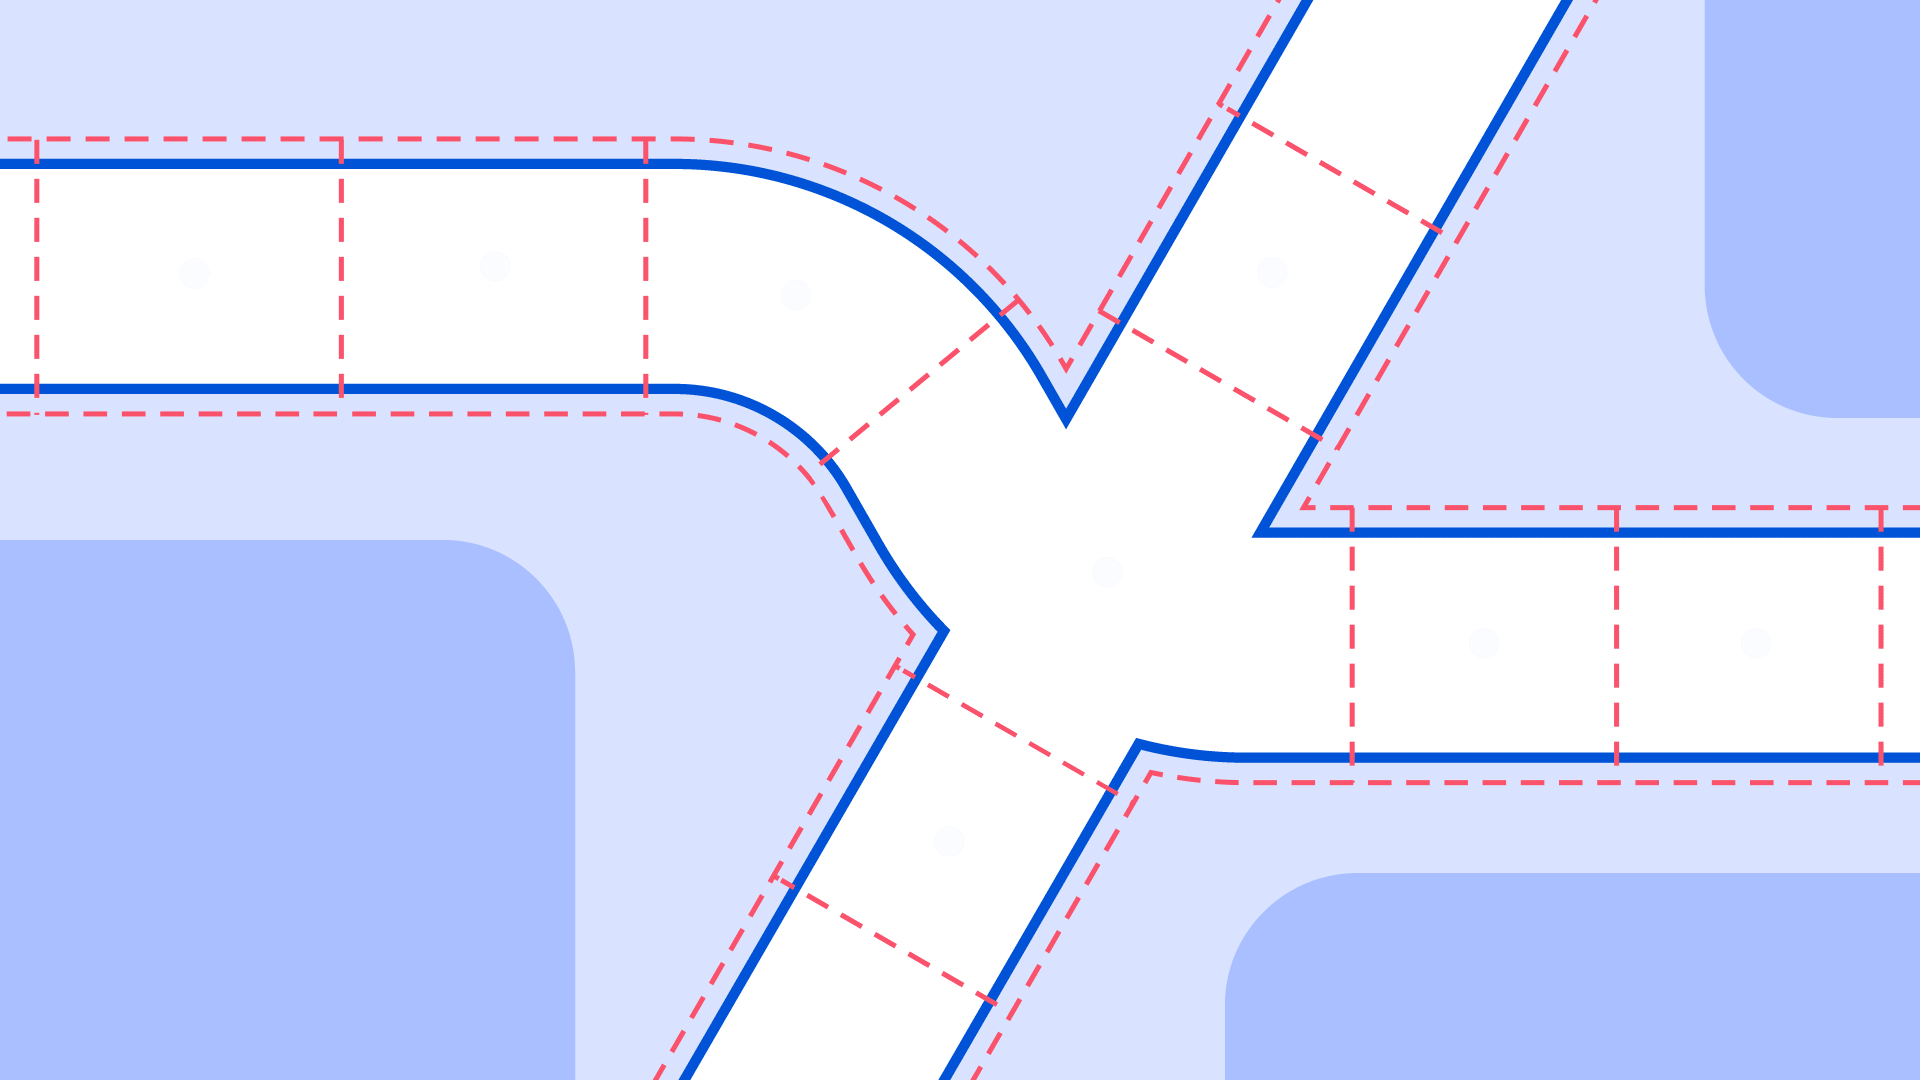
\includegraphics[width=\linewidth]{figures/superseg-1.png}\\ 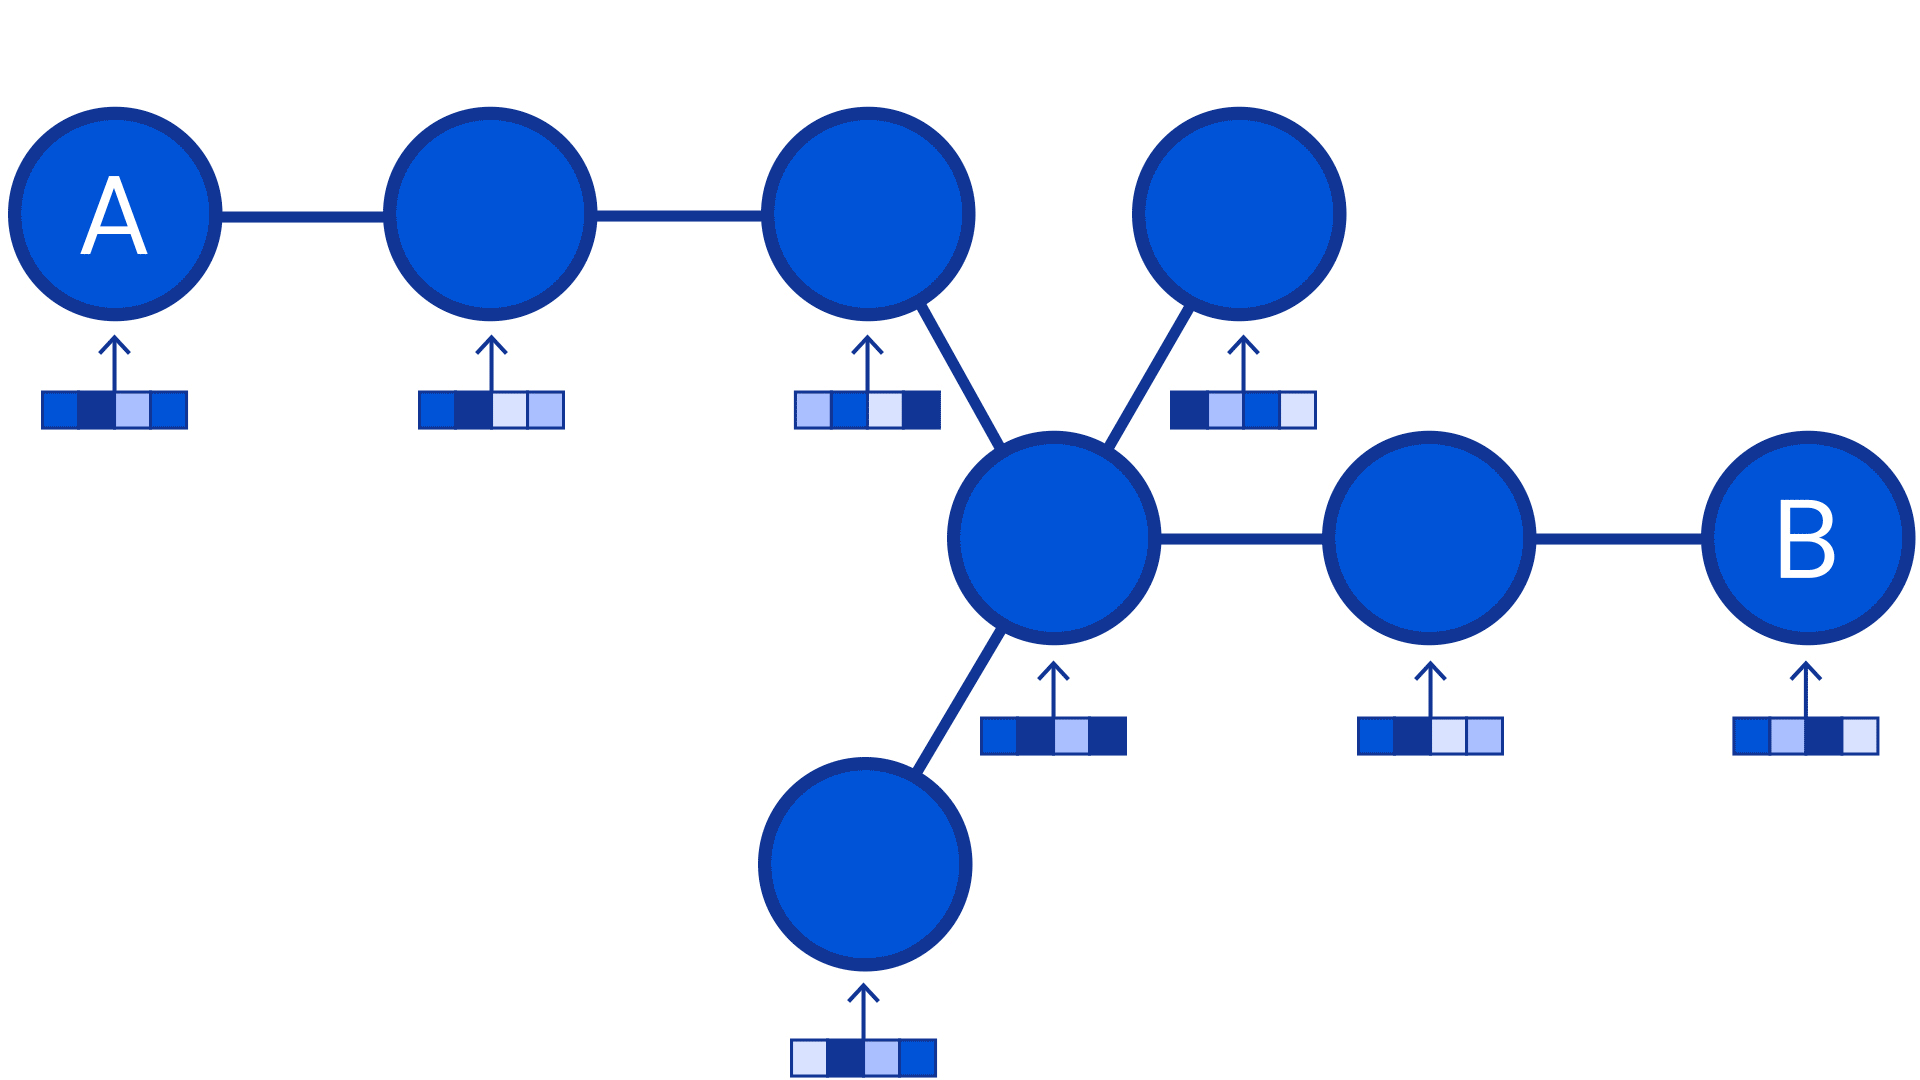
\includegraphics[width=\linewidth]{figures/superseg-3.png}\\ 道路网络（上）及其对应的图表示（下）。}例如，在道路网络上，可以把交叉路口视为节点，把连接它们的路段视为边；随后可用道路长度、路段当前或历史行驶速度等信息为这些边构造特征。

这一领域的标准预测问题之一是预测\emph{预计到达时间}（ETA）：对于给定的候选路线，提供走完该路线所需的预期行程时间。这个问题至关重要，不仅涉及面向用户的交通推荐应用，也关系到在自身运营中使用这类预测的企业（如外卖或网约车服务）。

图神经网络在这一领域同样展现出巨大潜力：例如，可直接预测道路网络相关子图的 ETA（实质上是一项\emph{图回归}任务）。\marginnote{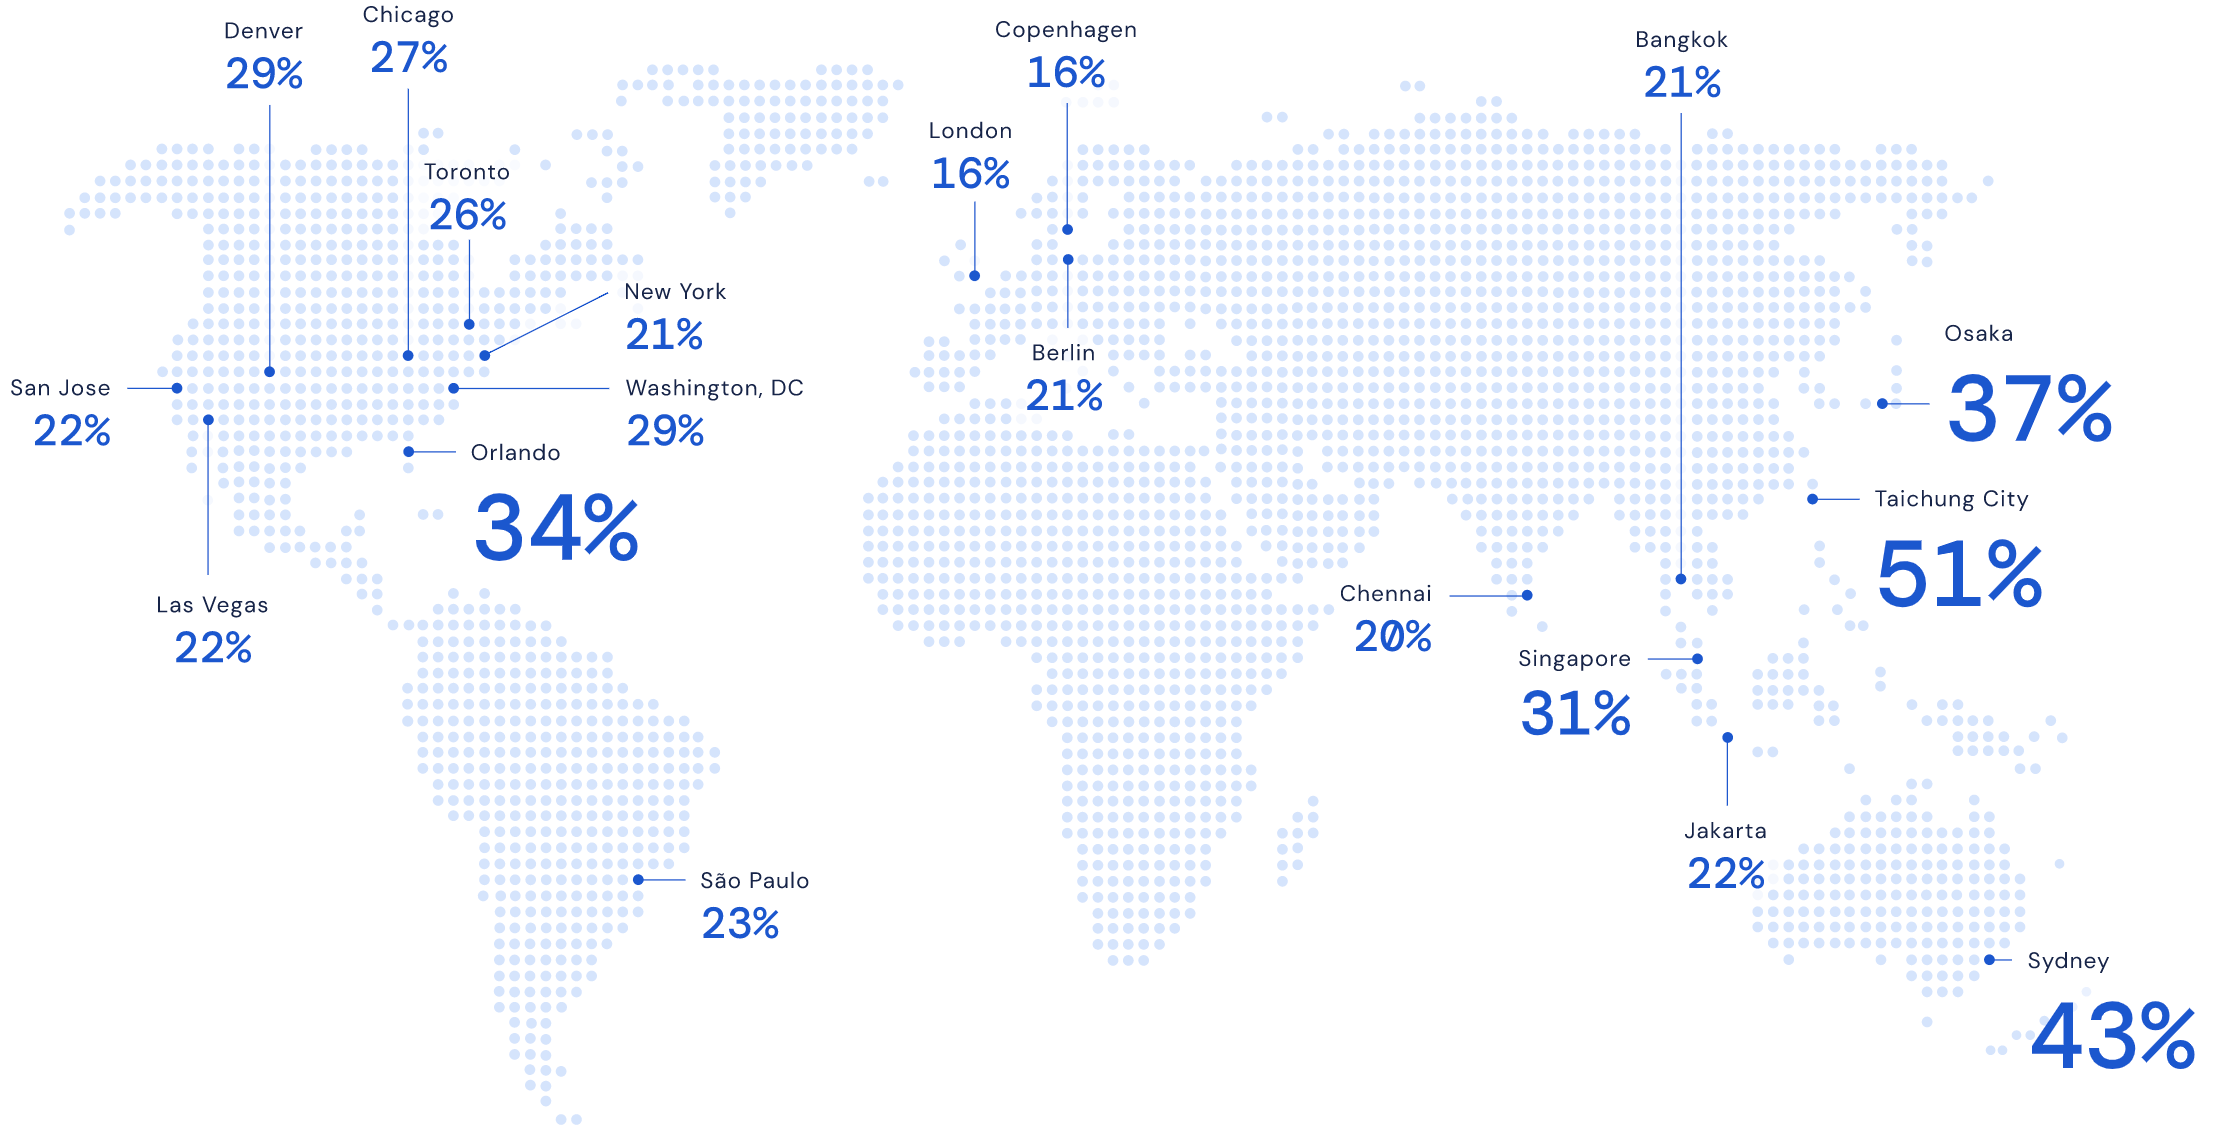
\includegraphics[width=\linewidth]{figures/maps-improvements.png}\\ Google Maps 中使用 GNN 响应查询的若干大都市区域，并标出了预测质量的相对提升（Sydney 等城市达到 40+\%）。}DeepMind 成功采用了这种方法，得到一个基于 GNN 的 ETA 预测器；该预测器现已部署在 Google Maps 的生产环境中，为全球多个主要都市区提供 ETA 查询服务 \citep{derrowpinion2021traffic}。Baidu Maps 团队也观察到类似收益；其行程时间预测目前由 ConSTGAT 模型提供，而该模型本身基于图注意力网络模型的一种时空变体 \citep{fang2020constgat}。

\paragraph{物体识别} 计算机视觉中机器学习技术的一项主要基准，是能否对给定图像中的中心物体进行\emph{分类}。\marginnote{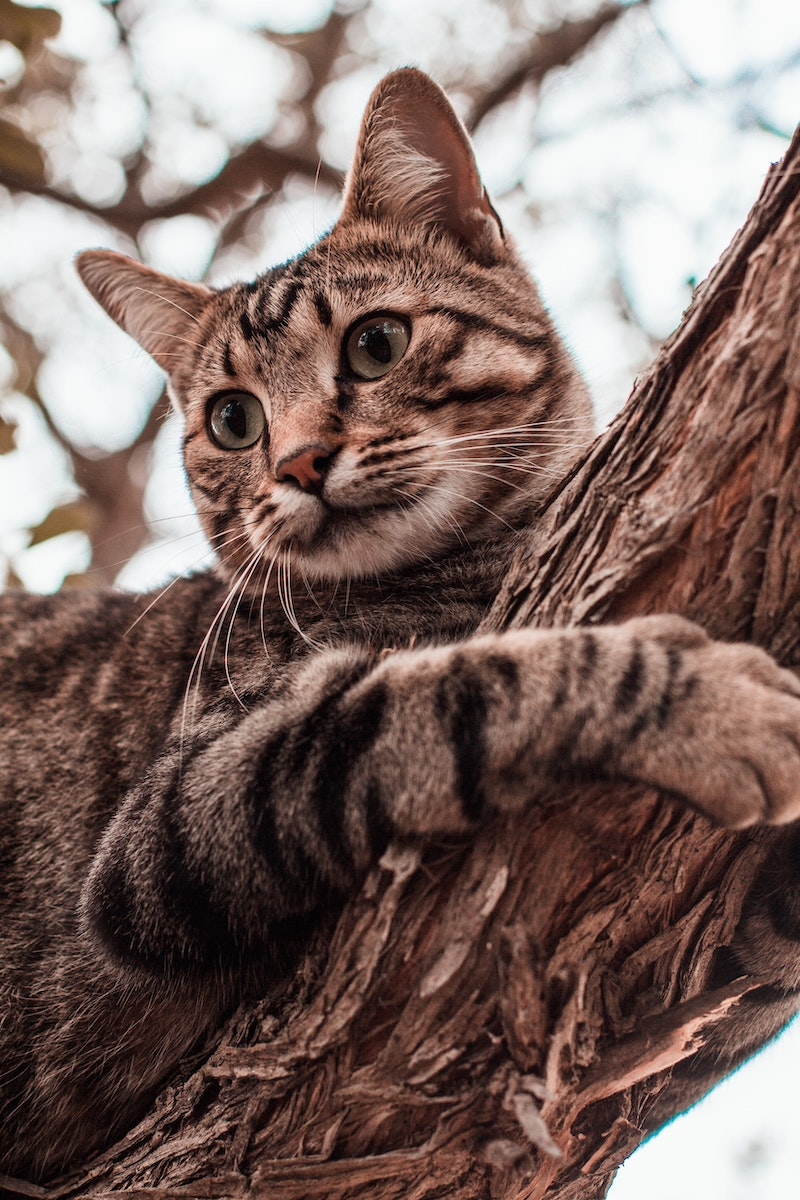
\includegraphics[width=\linewidth]{figures/tabby_cat.jpg}\\ 一幅输入图像示例；ImageNet 中可以找到类似图像，它表示\emph{“虎斑猫”}类别。}ImageNet 大规模视觉识别挑战赛 \citep[ILSVRC]{russakovsky2015imagenet} 是一项年度物体分类竞赛，推动了几何深度学习早期发展的很大一部分。ImageNet 要求模型把从 Web 抓取的真实图像分到 1000 个类别之一：这些类别既多样（涵盖有生命和无生命物体），又具体（许多类别着重区分不同的猫和犬品种）。因此，在 ImageNet 上表现良好往往意味着模型能够从一般照片中稳健地提取特征，这为从预训练 ImageNet 模型出发的各种\emph{迁移学习}设置奠定了基础。

卷积神经网络在 ImageNet 上的成功——尤其是 \citet{krizhevsky2012imagenet} 的 AlexNet 模型在 ILSVRC 2012 中以巨大优势夺冠——在很大程度上引领了整个深度学习在学术界和工业界的应用。此后，CNN 一直位居 ILSVRC 前列，并催生了许多流行架构，如 VGG-16 \citep{simonyan2014very}、\marginnote{有趣的是，VGG-16 架构有十六个卷积层，作者称其为“非常深”。随后的发展很快把这类模型扩展到数百层乃至数千层。}[5\baselineskip]Inception \citep{szegedy2015going} 和 ResNets \citep{he2016deep}；这些架构已在该任务上成功超越人类水平。这些架构采用的设计决策与正则化技术（如修正线性激活 \citep{nair2010rectified}、dropout \citep{srivastava2014dropout}、跳跃连接 \citep{he2016deep} 和批归一化 \citep{ioffe2015batch}）构成了当今许多有效 CNN 模型的基础。

在物体分类发展的同时，物体\emph{检测}也取得了显著进展；它要求分离出图像中所有感兴趣的物体，并为它们标注特定类别。该任务关系到从图像描述到自动驾驶汽车的多种下游问题。由于预测结果需要\emph{局部化}，它要求采用更细粒度的方法；因此，平移等变模型往往在这一领域体现出价值。一个有影响力的实例是 R-CNN 模型家族 \citep{girshick2014rich,girshick2015fast,ren2015faster,he2017mask}。在相关的\emph{语义分割}领域，\citet{badrinarayanan2017segnet} 的 SegNet 模型也颇具影响力，其编码器--解码器架构以 VGG-16 为骨干。

\paragraph{游戏博弈} 当观测状态能够表示在网格域上时，卷积神经网络也作为平移不变特征提取器，在\emph{强化学习}（RL）环境中发挥重要作用；例如，从像素学习玩电子游戏便属于这种情况。%\marginnote{\includegraphics[width=0.9\linewidth]{figures/mspacman.png} The \emph{Atari 2600} is an example of a video gaming system that has been heavily repurposed as an RL environment (primarily by the efforts of \citet{bellemare2013arcade}. Shown above is an image of \emph{Ms. Pacman}, one of the games supported therein.}.
%
在这种情况下，CNN 负责把输入约化为扁平向量表示，随后用该表示导出驱动 RL 智能体行为的\emph{策略}或\emph{价值函数}。尽管强化学习的具体细节并非本节重点，但需要指出，过去十年中一些最具影响力的深度学习成果来自以 CNN 为支撑的强化学习。

这里尤其值得提及的一个实例是 DeepMind 的 \emph{AlphaGo} \citep{silver2016mastering}。它把 CNN 应用于表示当前棋子位置的 $19\times 19$ 网格，从而编码围棋对局的当前状态。随后，通过结合学习既往专家棋步、Monte Carlo 树搜索和自我对弈，它成功达到足以在五局挑战赛中击败 Lee Sedol 的围棋水平；后者是有史以来最强的围棋棋手之一，这场比赛也得到了全球广泛报道。

这已经是更广泛人工智能领域的一个重要里程碑——围棋的状态空间远比国际象棋等游戏复杂。\marginnote{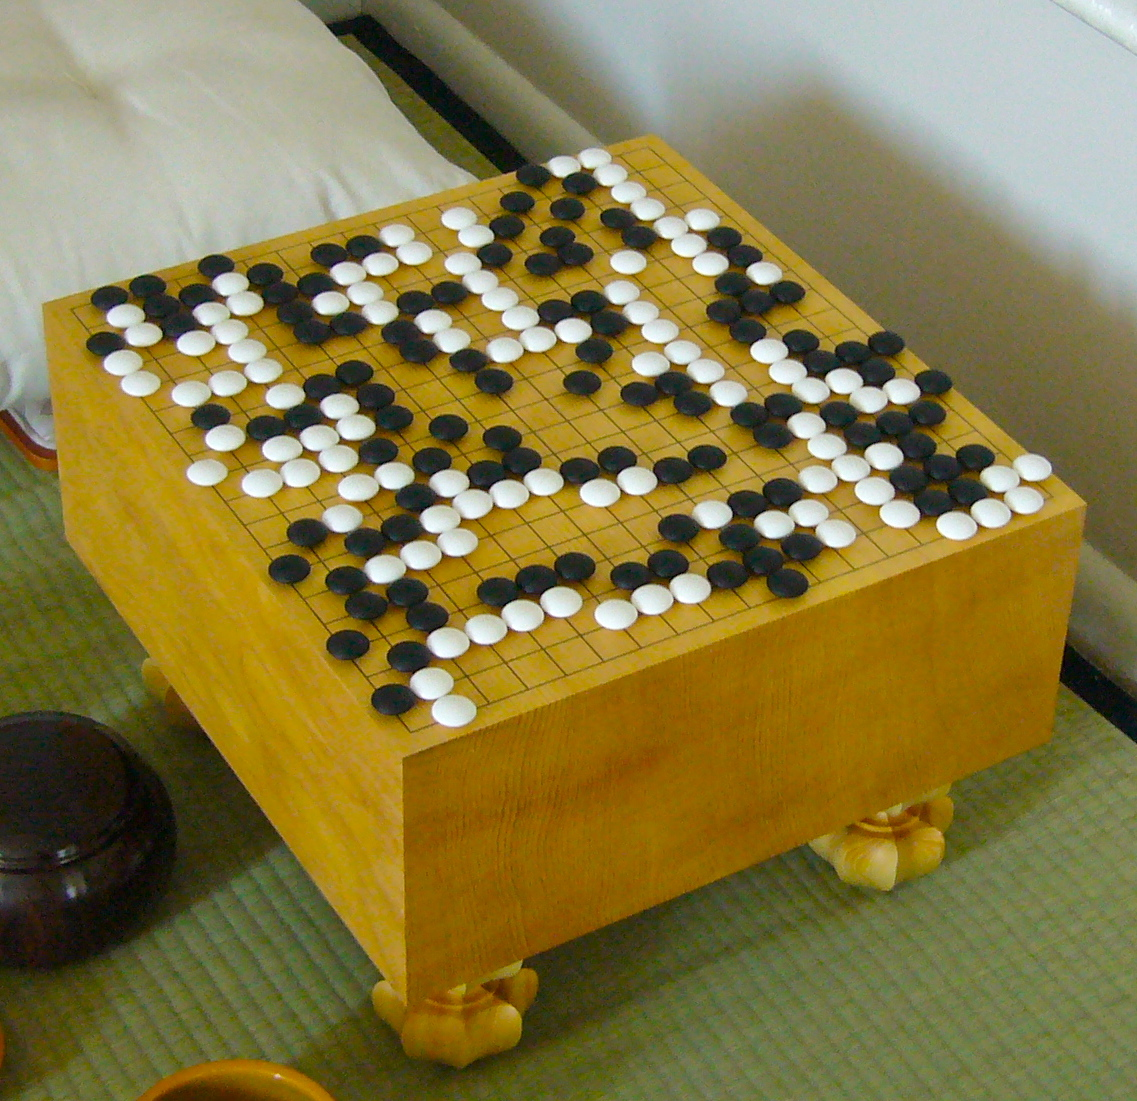
\includegraphics[width=\linewidth]{figures/Go_board.jpeg} 围棋在 $19\times 19$ 棋盘上进行，两名棋手在空位放置黑白\emph{棋子}。合法状态数估计为 $\approx2\times 10^{170}$ \citep{tromp2006combinatorics}，远远超过宇宙中的原子数。}但 AlphaGo 的发展并未就此止步。作者逐步从架构中移除越来越多围棋特有的偏置：\emph{AlphaGo Zero} 移除了人类偏置，仅通过自我对弈进行优化 \citep{silver2017mastering}；\emph{AlphaZero} 把该算法扩展到国际象棋和将棋等相关双人游戏；最后，\emph{MuZero} \citep{schrittwieser2020mastering} 纳入了一个能够即时\emph{学习}游戏规则的模型，从而在没有任何先验规则知识的情况下，在 Atari 2600 游戏以及围棋、国际象棋和将棋上取得强劲性能。在所有这些发展过程中，CNN 始终是这些模型表示输入的骨干。

多年来，人们为 Atari 2600 平台提出了多个高性能 RL 智能体 \citep{mnih2015human,mnih2016asynchronous,schulman2017proximal}，但它们长期无法在该平台提供的\emph{全部} 57 款游戏上达到人类水平。Agent57 \citep{badia2020agent57} 最终突破了这一障碍：它使用从强探索性到纯利用性的参数化策略族，并在不同训练阶段以不同方式确定这些策略的优先级。它的大部分计算同样由作用于电子游戏帧缓冲区的 CNN 完成。

\paragraph{文本与语音合成} 除了自然映射到\emph{二维}网格的图像之外，（几何）深度学习的一些重大成功发生在一维网格上。\emph{文本}和\emph{语音}便是自然的例子，它们把几何深度学习蓝图带入自然语言处理和数字信号处理等不同领域。

这一领域中应用最广、报道最多的一些工作聚焦于\emph{合成}：无条件地，或以特定\emph{提示}为条件，生成语音或文本。这种设置可以支持大量实用任务，如\emph{文本转语音}（TTS）、预测式文本补全和机器翻译。过去十年中，人们提出了多种文本与语音生成神经架构；早期方案大多基于\emph{循环}神经网络，例如前述 seq2seq 模型 \citep{sutskever2014sequence} 或循环注意力 \citep{bahdanau2014neural}。然而，近年来它们逐渐被卷积神经网络和基于 Transformer 的架构取代。

这一设置中，简单 1D 卷积的一项特有限制是其\emph{感受野}线性增长，因而需要许多层才能覆盖此前已经生成的序列。相比之下，\emph{空洞}卷积\marginnote{空洞卷积也称为 \emph{\`{a} trous} 卷积（该法语词组字面意为“带孔的”）。}能以相同数量的参数提供\emph{指数增长}的感受野。凭借这一点，它成为非常有力的替代方案，最终在机器翻译上达到可与 RNN 竞争的水平 \citep{kalchbrenner2016neural}；同时，由于能够在所有输入位置并行计算，它还大幅降低了计算复杂度。\marginnote{这类技术在蛋白质--蛋白质相互作用等不同问题上也超过了 RNN \citep{deac2019attentive}。}空洞卷积最知名的应用是 \cite{oord2016wavenet} 提出的 \emph{WaveNet} 模型。WaveNet 证明，利用空洞可以在\emph{原始波形}层面（通常每秒 16,000 个或更多采样点）合成语音，所生成的语音样本比此前最好的文本转语音（TTS）系统明显更“像人”。\marginnote{除此之外，WaveNet 模型还被证明能够生成钢琴曲。}随后，研究进一步表明，可以把 WaveNet 的计算蒸馏到简单得多的 \emph{WaveRNN} 模型 \citep{kalchbrenner2018efficient} 中；该模型使这项技术能够有效地实现工业规模部署。这不仅使其能够用于 Google Assistant 等服务的大规模语音生成，也使 Google Duo 等使用端到端加密的应用能够在设备端高效计算。

Transformer \citep{vaswani2017attention} 成功突破了循环架构与卷积架构的限制，表明仅凭\emph{自注意力}即可在机器翻译中取得最先进性能。随后，Transformer 给自然语言处理带来了革命性变化。借助 BERT \citep{devlin2018bert} 等模型提供的预训练嵌入，Transformer 计算得以用于大量自然语言处理下游应用；例如，Google 使用 BERT 嵌入为其搜索引擎提供支持。

过去几年中，Transformer 得到最广泛报道的应用或许是文本生成；这一方向主要由 OpenAI 的\emph{生成式预训练 Transformer}（GPT，\cite{radford2018improving,radford2019language,brown2020language}）模型家族推动。特别是，GPT-3 \citep{brown2020language} 成功把语言模型学习扩展到 1750 亿个可学习参数，并使用 Web 规模的抓取文本语料进行下一词预测训练。这使它不仅成为能在多种语言任务上发挥强大作用的少样本学习器，还成为能够生成连贯且近似人类表达的文本生成器。这种能力既带来了大量下游应用，也引发了广泛的媒体报道。

\paragraph{医疗健康}
%
医疗领域的应用是几何深度学习另一个前景可期的方向。这些方法正以多种方式得到使用。
%
首先，CNN 等较传统的架构已被应用于网格结构数据，例如用于
预测重症监护病房的住院时长
\citep{rocheteau2020temporal}, 
或根据视网膜扫描诊断威胁视力的疾病 \citep{de2018clinically}。
%
\cite{winkels2019pulmonary} 表明，与常规 CNN 相比，使用 3D 旋转--平移群卷积网络能够提高
肺结节检测的准确率。


其次，把器官建模为几何曲面后，网格曲面卷积神经网络已被证明能够处理多种任务，包括根据遗传学相关信息重建面部结构 \citep{mahdi20203d}、
大脑皮层分区 \citep{cucurull2018convolutional}，以及
根据皮层表面结构回归人口统计学属性 \citep{besson2020geometric}。
%
%The latter problems consists of []
%Third, 
%
后一组例子体现了神经科学中日益明显的一种趋势：把大脑视为具有复杂褶皱的曲面，\marginnote{在解剖学文献中，大脑皮层的这类结构称为\emph{脑沟}和\emph{脑回}。}由此产生高度非 Euclidean 的结构。
%since the data in this field are often represented on surface models of the brain. 
%as many cortical properties only make sense considering their specific location with respect to the various sulci and gyri [8]. These surface models are essentially sheet-like meshes that are intricately folded in three-dimensional space, maintaining the geometrical structure of the brain


与此同时，
神经科学家经常尝试构建并分析大脑的\emph{功能网络}，表示执行某种认知功能时共同激活的各个脑区；这些网络通常用功能磁共振成像（fMRI）构建，该技术实时显示大脑哪些区域消耗了更多血液。\marginnote{通常使用血氧水平依赖（BOLD）对比成像。}
%
这些功能网络既可以揭示患者的人口统计学特征（例如区分男性与女性，\cite{arslan2018graph}），也可以用于神经病理诊断；后者是我们要在此强调的几何深度学习在医学中的第三类应用。在这一背景下，\cite{ktena2017distance} 率先使用图神经网络预测孤独症谱系障碍等神经系统疾病。
%
大脑的几何结构与功能结构似乎密切相关，近期 \cite{itani2021combining} 指出，在神经系统疾病分析中联合利用二者是有益的。
% can reveal important information about the complexity of the neuropathology


第四，\emph{患者网络}在基于 ML 的医学诊断中正变得更加重要。这类方法的基本依据是，患者在人口统计学、基因型和表型上的相似性信息可能有助于改善疾病预测。
%
 \cite{parisot2018disease}
 把图神经网络应用于由人口统计学特征构建的患者网络，以诊断神经系统疾病，并表明使用图能够改善预测结果。
 %
\cite{cosmo2020latent} 展示了潜在图学习（即由网络\emph{学习}未知的患者图）在这一设置中的益处。后一项工作使用了 UK Biobank 的数据；这是一个包含脑成像在内的大规模医学数据集合 \citep{miller2016multimodal}。




医院患者的大量数据可以在\emph{电子健康记录}（EHR）中找到。\marginnote{公开可用的匿名重症监护 EHR 数据集包括 MIMIC-III \citep{johnson2016mimic} 和 eICU \citep{pollard2018eicu}。}EHR 分析不仅能够全面呈现患者的病情发展，还能把相似患者\emph{关联}起来。这与诊断中常用的\emph{模式识别法}一致：临床医生凭借\emph{经验}识别临床特征模式；当医生的经验使其能够迅速诊断病情时，这可能就是所采用的主要方法。沿着这一思路，多项工作尝试基于 EHR 数据构建患者图，其依据可以是医生记录的嵌入 \citep{malone2018learning}、入院时诊断的相似性 \citep{rocheteau2021predicting}，甚至可以假定一个全连接图 \citep{zhu2019graph}。在所有这些情形中，使用图表示学习处理 EHR 都展现出了有前景的结果。



\paragraph{粒子物理学与天体物理学}
高能物理学家或许是自然科学领域最早接纳图神经网络这一崭新工具的专业群体之一。
%
在近期的一篇综述中，\cite{shlomi2020graph} 指出，\marginnote{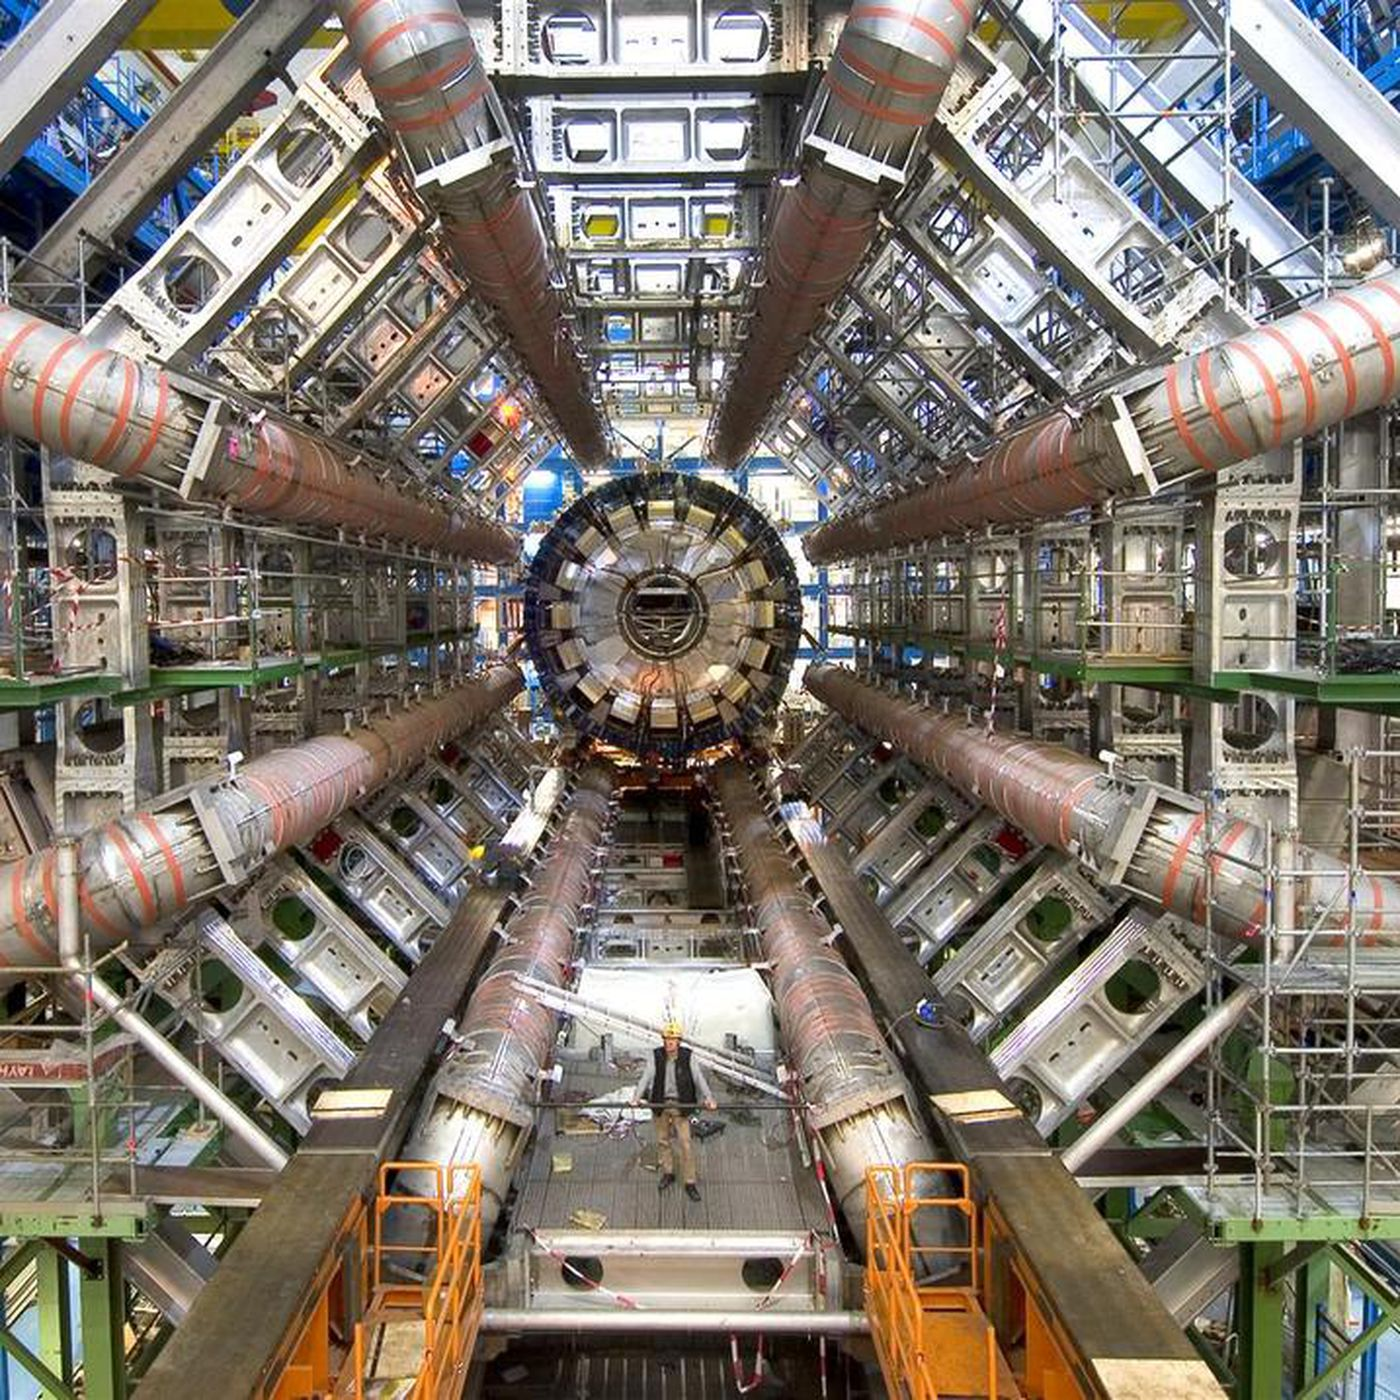
\includegraphics[width=\linewidth]{figures/lhc.jpeg}
Large Hadron Collider 探测器的一部分。
}机器学习在粒子物理实验中历来得到广泛使用：或者学习复杂的逆函数，以便从探测器测得的信息推断底层物理过程；或者执行分类与回归任务。对于后一类任务，为了能够使用 CNN 等标准深度学习架构，往往必须强行把数据转化为网格等不自然的表示。然而，物理学中的许多问题涉及无序集合形式的数据，其中包含丰富的关系与相互作用，因此可以自然地表示为图。


高能物理学的一项重要应用是重建并分类\emph{粒子喷注}——它们是稳定粒子形成的喷流，%that are stemming
源于某一初始事件所产生粒子的多次连续相互作用与衰变。
% (for example, a collision of ).
%
在 CERN 建造的最大、最著名的粒子加速器 Large Hadron Collider 中，这类喷注源自以接近光速运动的质子之间的碰撞。
%ccelerated to a speed close to that of light, they collide with other protons. 
这些碰撞会产生有质量粒子，例如长期以来人们一直在寻找的 Higgs 玻色子或顶夸克。
%
%object. 
%
识别并分类碰撞事件至关重要，因为这可能为新粒子的存在提供实验证据。


近期，人们为粒子喷注分类任务提出了多种几何深度学习方法；\marginnote{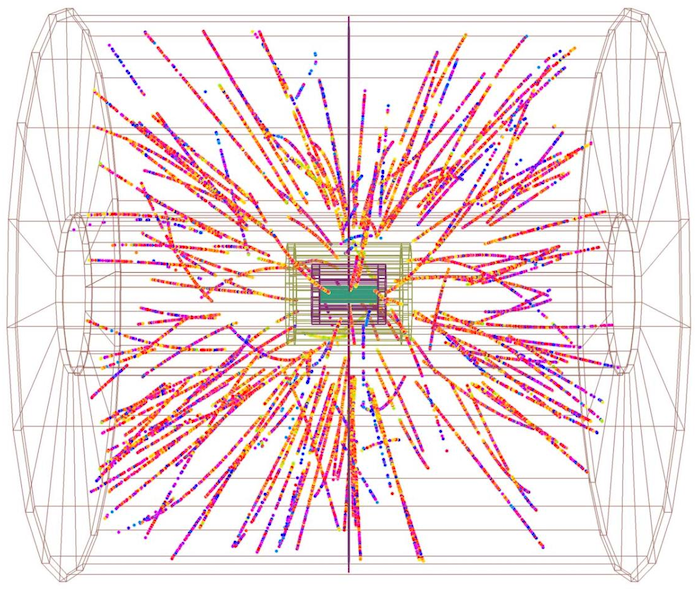
\includegraphics[width=\linewidth]{figures/particlejet.png}
粒子喷注示例。
}例如，\cite{komiske2019energy} 和 \cite{qu1902particlenet} 分别提出了基于 DeepSet 和 Dynamic Graph CNN 架构的方法。
%
%Recently GNNs have been extended by adding inductive biases
近来，人们还对开发源于物理学考虑的专门架构产生了兴趣：这类架构可以纳入与 Hamilton 或 Lagrange 力学一致的归纳偏置（例如见 \cite{sanchez2019hamiltonian,cranmer2020lagrangian}），对 Lorentz 群（物理学中时空的一项基本对称性）保持等变 \citep{bogatskiy2020lorentz}，甚至纳入符号推理 \citep{cranmer2019learning}，并能够从数据中学习物理定律。这类方法更具可解释性（因而被领域专家视为更“可信”），也具有更好的泛化能力。



除了粒子加速器之外，
天体物理学家如今还把粒子探测器用于\emph{多信使天文学}——这是一种协调观测来自同一信号源的电磁辐射、引力波和中微子等不同信号的新方式。
%
中微子天文学尤其引人关注，因为中微子极少与物质发生相互作用，因而能够几乎不受影响地传播极远距离。\marginnote{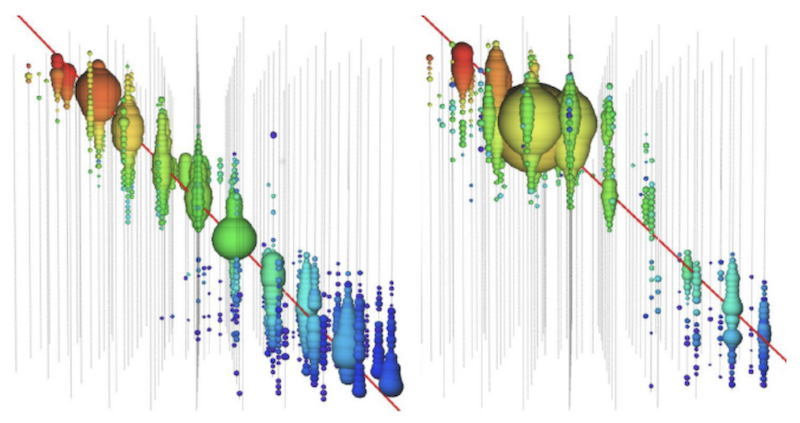
\includegraphics[width=\linewidth]{figures/icecube.png} IceCube 探测器中背景事件（左：muon 束）
与天体物理中微子（右：高能单 muon）形成的特征性光沉积分布。\cite{choma2018graph}
}探测中微子可以观测光学望远镜无法观测的对象，但需要规模极其庞大的探测器——IceCube 中微子观测站使用南极点一立方千米的南极冰架作为探测器。
%
探测高能中微子可能有助于揭示宇宙中一些最神秘的对象，例如耀变体和黑洞。
%
\cite{choma2018graph} 使用几何神经网络建模 IceCube 中微子探测器的不规则几何结构，在探测来自天体物理源的中微子并将其与背景事件分离方面展现出显著更好的性能。


尽管中微子天文学在宇宙研究中前景广阔，传统光学望远镜和射电望远镜仍然是天文学家的主力工具。
%
即使使用这些传统仪器，几何深度学习仍能为数据分析提供新方法。例如，\cite{scaife2021fanaroff} 使用旋转等变 CNN 对射电星系进行分类，\cite{mcewen2021scattering} 则使用
球面 CNN 分析宇宙微波背景辐射；后者是 Big Bang 的遗迹，可能有助于揭示早期宇宙的形成。正如前面提到的，这类信号自然地表示在球面上，而等变神经网络是研究它们的适当工具。


%\michael{TACO: anything on the sphere? There is a work of Defferard, but I don't like it because they use GNNs on the meshed sphere, which is non comme il faut}

%[47], which can improve performance and generalization on various physical
%prediction problems. Other recent work [7] has shown symbolic physical laws can be
%extracted from the learned functions within a GN.


%For additional details on various applications of Geometric Deep Learning in particle physics, we refer the reader to a recent review by \cite{shlomi2020graph}. 



\paragraph{虚拟现实与增强现实}
另一个推动大量几何深度学习方法发展的应用领域是计算机视觉与图形学，尤其是面向虚拟现实和增强现实的 3D 人体模型处理。
%
用于制作 Avatar 等电影特效的动作捕捉技术通常分两个阶段运行：首先，把捕捉演员身体或面部动作的 3D 扫描仪输入与某个规范形状建立对应关系；该形状通常建模为离散流形或网格曲面（这一问题常称为“分析”）。其次，生成一个新形状来复现输入的动作（“合成”）。
%
计算机图形学与视觉中关于几何深度学习的早期工作 \citep{masci2015geodesic,boscaini2016learning,monti2017geometric} 开发了网格曲面卷积神经网络，用于解决分析问题，更具体地说，是可形变形状对应问题。


\cite{litany2018deformable} 和 \cite{ranjan2018generating} 分别独立提出了最早用于 3D 形状合成的几何自编码器架构。在这些架构中，假定身体、面部或手部的规范网格曲面已知，而合成任务则是回归节点的 3D 坐标（用微分几何术语说，即曲面的嵌入）。%,bouritsas2019neural}.
%
\cite{kulon2020weakly} 展示了一条用于 3D 手部姿态估计的混合流水线，它采用基于图像 CNN 的编码器和几何解码器。\marginnote{ 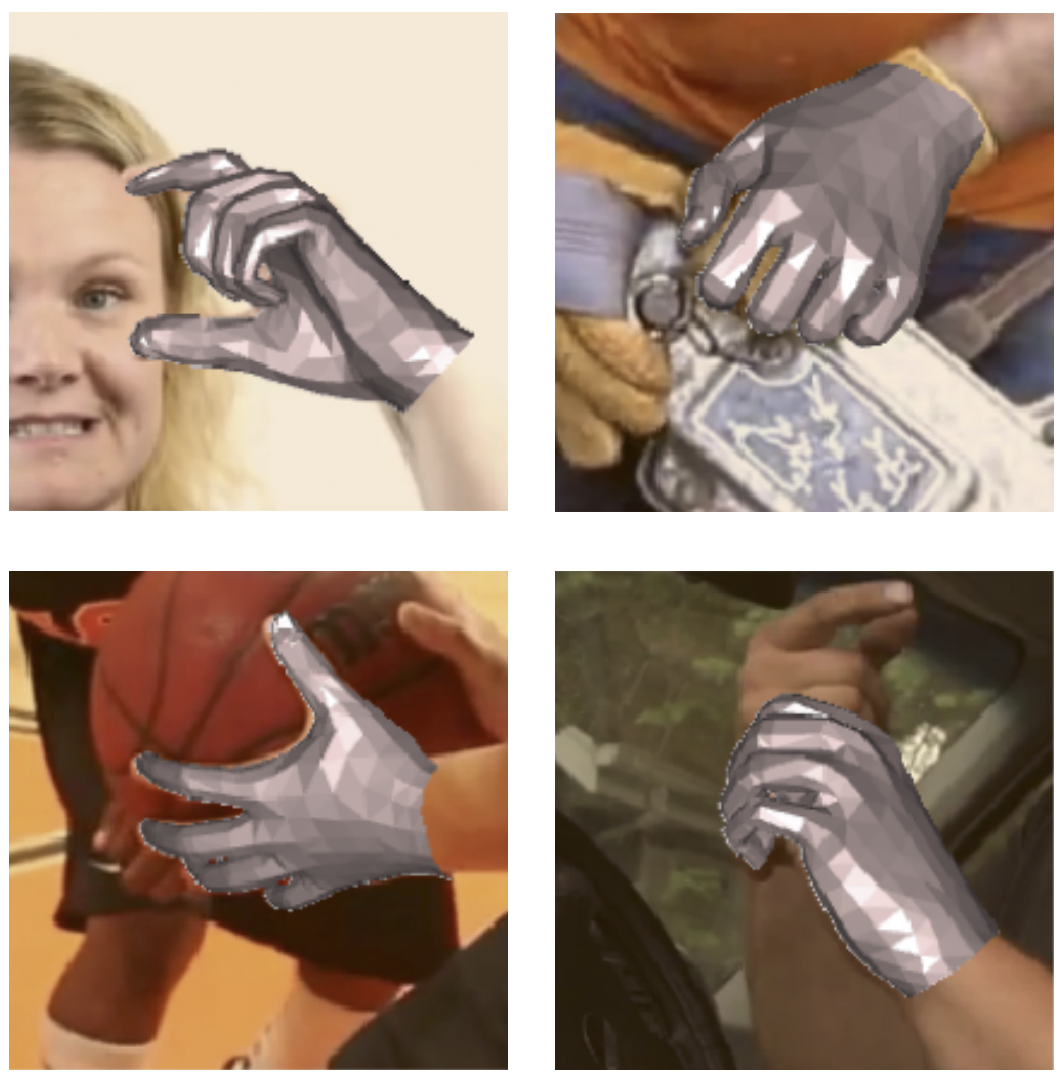
\includegraphics[width=\linewidth]{figures/ariel.png}\\ 从自然场景 2D 图像重建复杂 3D 手部姿态的示例 \citep{kulon2020weakly}。}该系统与英国初创公司 Ariel AI 合作开发，并在 CVPR 2020 上演示；它能够根据手机视频输入，以快于实时的速度创建具有完全关节化双手的逼真人体化身。%
Ariel AI 于 2020 年被 Snap 收购；在本文写作时，其技术已用于 Snap 的增强现实产品。
%Shape correspondence, Protein molecular surfaces, Ariel AI


\section{历史视角}

“无论你把对称的含义定义得多么宽泛或狭窄，它都是人类自古以来试图理解并创造秩序、美与完美所凭借的一种观念。”\marginnote{
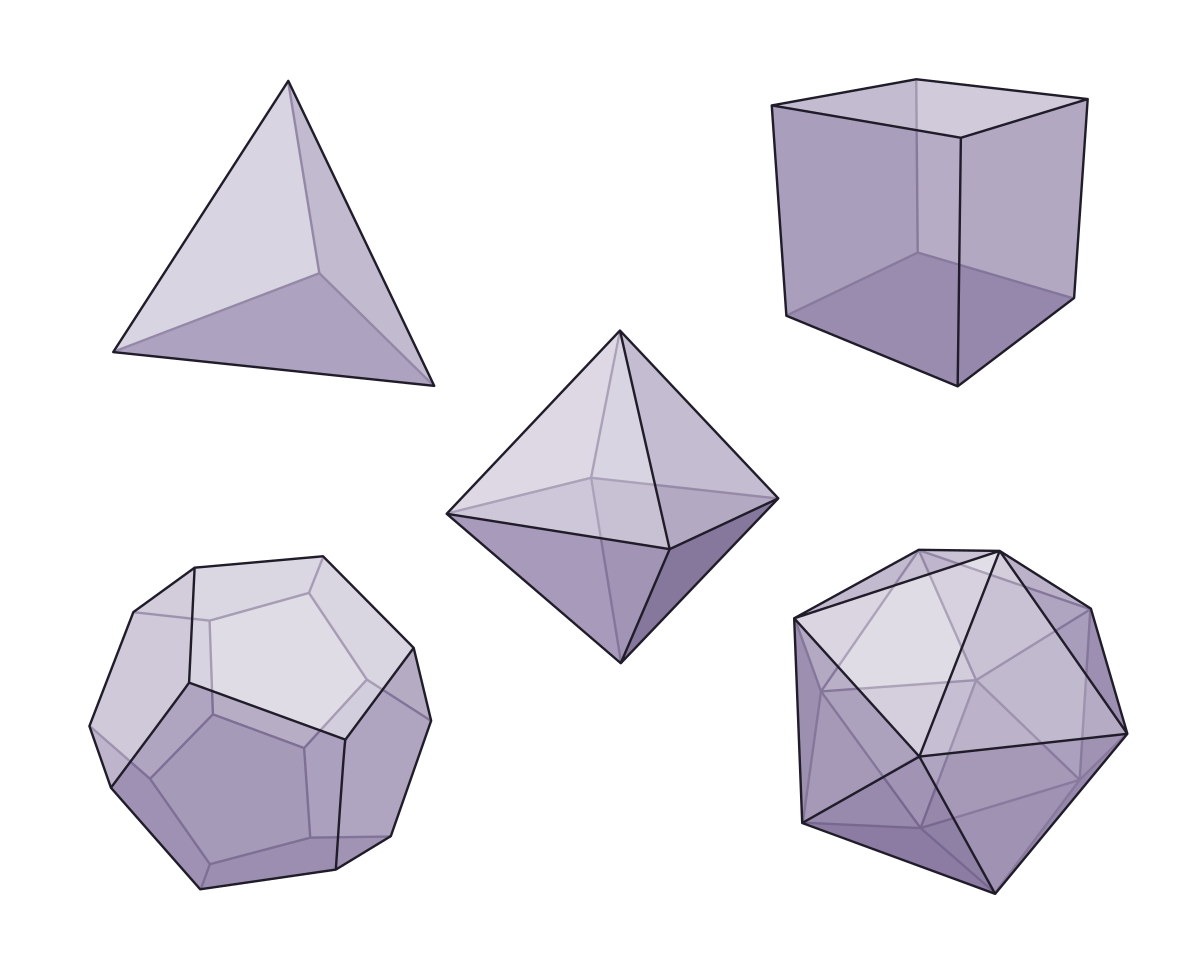
\includegraphics[width=0.9\linewidth]{figures/platonic_solids.png}
四面体、立方体、八面体、十二面体和二十面体称为\emph{Platonic 立体}。}
%
这个略带诗意的对称定义，出自伟大数学家 Hermann \citet{weyl2015symmetry} 的同名著作；那是他从 Princeton Institute for Advanced Study 退休前夕的\emph{绝唱}。
%
Weyl 追溯了对称自古以来在科学与艺术中的特殊地位，从 Sumerian 的对称设计，到因圆具有旋转对称性而认为它是完美形状的 Pythagoreans。
%
Plato 认为，今天以他命名的五种正多面体具有如此基础的地位，以至于它们必定是塑造物质世界的基本构件。
%
不过，尽管人们认为 Plato 创造了术语 \textgreek{summetr'ia}（字面意为“相同的尺度”），他只是含糊地用它表达艺术中比例之美与音乐中的和谐。
%
天文学家兼数学家 Johannes Kepler 首次尝试对水晶体的对称形状作严格分析。在他的论著《六角雪花》中，\marginnote{
%\includegraphics[width=0.9\linewidth]{figures/de_nive.png}
其完整书名为
\emph{Strena, Seu De Nive Sexangula}（“新年礼物，或论六角雪花”）；正如标题所暗示的，这是 Kepler 于 1611 年作为圣诞礼物寄给资助者兼友人 Johannes Matthäus Wackher von Wackenfels 的一本小册子。}他把雪花的六重二面体结构归因于粒子的六角密堆积；尽管这一观念早于人们对物质形成方式的清晰认识，却至今仍是晶体学的基础 \citep{ball2011retrospect}。




%D'Arcy Thompson {\em On Growth and Form} appeals to the notions of symmetry to explain the structure of biological life forms. 

\paragraph{数学与物理学中的对称性}
在现代数学中，对称性几乎毫无例外地用群论语言表达。%
这一理论的起源通常归功于 {\'E}variste Galois；他创造了这个术语，并在 19 世纪 30 年代用它研究多项式方程的可解性。
%
另外两个与群论相关的名字是 Sophus Lie 和 Felix Klein；二人曾经相识，并在一段时期内开展了富有成效的合作 \citep{tobies2019felix}。前者后来发展了今天以其名字命名的连续对称性理论；后者则在本文开头提到的 Erlangen Programme 中宣称群论是组织几何学的原则。Riemann 几何被明确排除在 Klein 的统一几何图景之外，直到五十年后才被纳入其中，这在很大程度上得益于 {\'E}lie Cartan 在 20 世纪 20 年代的工作。

%unified multiple geometries. 

%Physics:  


Klein 在 G\"ottingen 的同事 Emmy Noether 证明，物理系统作用的每一种可微对称性都有相应的守恒律 \citep{variationsprobleme1918nachr}。这在物理学中是一项惊人的结果：在此之前，发现能量守恒等基本定律需要细致的实验观测，即便如此，得到的也只是没有理论来源的经验结果。Noether 定理——用诺贝尔奖得主 Frank Wilczek 的话说，是“20 与 21 世纪物理学的指路明星”——表明能量守恒源于时间的平移对称性。这一观念相当直观：实验结果不应取决于实验是在今天还是明天进行。

%That theorem has been a guiding star to 20th and 21st century physics,” says theoretical physicist Frank Wilczek


%[FROM WIKI]
与电荷守恒相关的对称性，是电磁场的全局\emph{规范不变性}；\marginnote{Weyl 于 1919 年首次提出一个后来证明不正确的猜想：尺度或“规范”变化下的不变性是电磁学的一种局部对称性。术语 \emph{gauge}（德语为 \emph{Eich}）是类比铁路的不同轨距而选定的。%Although Weyl's choice of the gauge was initially incorrect, the name ``gauge'' stuck to the approach, and
量子力学发展之后，\cite{weyl1929elektron} 用波相位变化取代尺度因子，修正了规范的选择。见 \cite{straumann1996early}。
}它最早出现在 Maxwell 对电动力学的表述中 \citep{maxwell1865viii}；%This symmetry is related to the fact that the electric and magnetic fields are not changed by different choices of the value representing the zero point of electrostatic potential;
然而，其重要性最初并未受到注意。% in the earliest formulations.
%
%Similarly unnoticed was Hilbert's derivation of Einstein's equations of general relativity by postulating a symmetry under any change of coordinates. 
同一位 Hermann Weyl，
也就是那位以如此热烈的笔调书写对称性的人，%at the end of his academic career
在 20 世纪初首次把规范不变性概念引入物理学，并强调它是一条可以从中\emph{推导}出电磁学的
%symmetry
原理。
%
几十年后，这条基本原理才以其推广形式
%to non-Abelian gauge groups 
——由 \cite{yang1954conservation} 发展——
成功提供了一个统一框架，用于描述电磁作用、弱相互作用和强相互作用的量子力学行为，并最终形成 Standard Model；它涵盖了除引力之外的所有自然界基本力。
%
因此，我们可以赞同另一位诺贝尔奖得主、物理学家 Philip \cite{anderson1972more} 的结论：“说物理学就是对称性的研究，只是稍有夸张。”
%More is Different

% N. Strauman, Early History of Gauge Theories and Weak Interactions




%\michael{[from Taco's thesis]

\paragraph{机器学习中对称性的早期应用}
在机器学习及其模式识别与计算机视觉应用中，对称性的重要性早已得到认识。
%
\citet{amari1978feature}、\citet{kanatani2012group} 和 \citet{lenz1990group} 完成了为模式识别设计等变特征检测器的早期工作。\marginnote{Shun'ichi Amari 被认为是\emph{信息几何}领域的创始人；该领域把 Riemann 几何模型应用于概率。信息几何研究的主要对象是\emph{统计流形}，其中每个点对应一个概率分布。}
%
在
神经网络文献中，\citet{minsky2017perceptrons} 著名的感知机群不变性定理，对（单层）感知机学习不变量的能力
施加了根本限制。这是研究多层架构的主要动机之一 \citep{sejnowski1986learning,shawe1989building,shawe1993symmetries}，并最终促成了深度学习。

在神经网络界，\emph{Neocognitron} \citep{fukushima1982neocognitron} 被认为首次在神经网络中实现了平移不变性，用于“不受位置平移影响的模式识别”。
%maybe without explicitly realizing this fact. In his influential paper (Fukushima 1980) he laments of the response of perceptrons being ``severely affected by the shift in position and by the distortion in shape of the input patterns'' and concludes that ``their ability for pattern recognition was not so high.'' 
%
他的解决方案是一种具有局部连通性的层次神经网络，其灵感来自神经科学家 David Hubel 和 Torsten Wiesel 在二十年前于视觉皮层中发现的感受野 \citep{hubel1959receptive}。\marginnote{这项经典工作获得了 1981 年诺贝尔医学奖，Hubel 和 Wiesel 与 Roger Sperry 共同获奖。}
%
这些观念最终在 Yann LeCun 及其合作者的开创性工作 \citep{lecun1998gradient} 中发展为卷积神经网络。
%
\citet{wood1996representation} 首次从表示论视角研究不变与等变神经网络；遗憾的是，这项工作很少被引用。
%
这些观念较新的体现包括 \citet{makadia2007correspondence,esteves2020spin} 的工作
以及本文一位作者的工作 \citep{cohen2016group}。










%Convolutional neural networks: 



%Shawe-Taylor group equivariance
\paragraph{图神经网络}
%As to Graph Neural Networks, 
很难准确指出图神经网络这一概念从何时开始出现：一方面，多数早期工作并未把图作为一等对象；另一方面，GNN 直到 2010 年代末才变得实用；此外，这一领域本就源于多个研究方向的汇合。尽管如此，图神经网络的早期形式至少可以追溯到 20 世纪 90 年代，例如 Alessandro Sperduti 的 Labeling RAAM \citep{sperduti1994encoding}、%K\"{u}chler and Goller
\cite{goller1996learning} 的“通过结构反向传播”，以及数据结构的自适应处理方法%by Alessandro Sperduti, Antonina Starita and Paolo Frasconi
\citep{sperduti1997supervised,frasconi1998general}。这些工作主要关注在“结构”（通常是树或有向无环图）上进行运算，但其架构保持的许多不变性与当今更常用的 GNN 十分类似。



对一般图结构处理的首次严格研究（以及术语\emph{“图神经网络”}的提出）发生在 21 世纪之初。\marginnote{与此同时，Alessio Micheli 提出了\emph{图上的神经网络}（NN4G）模型；该模型关注\emph{前馈}范式，而不是循环范式 \citep{micheli2009neural}。}在意大利 Universit\`{a} degli Studi di Siena 的人工智能实验室中，由 Marco Gori 和 Franco Scarselli 领衔的论文提出了首个“GNN”\citep{gori2005new,scarselli2008graph}。这些模型依赖循环机制，要求神经网络参数指定\emph{压缩映射}，并通过寻找不动点来计算节点表示；这本身又需要一种特殊形式的反向传播 \citep{almeida1990learning,pineda1988generalization}，而且完全不依赖节点特征。\cite{li2015gated} 的 Gated GNN（GGNN）模型纠正了上述所有问题。GGNN 把现代 RNN 的许多优点带入 GNN 模型，如门控机制 \citep{cho2014learning} 和随时间反向传播，至今仍很流行。


\paragraph{计算化学}
还必须注意 GNN 的另一条独立且并行的发展路线：它完全由计算化学的需求推动；在这一领域，
分子最自然地表示为由化学键（边）连接原子（节点）所构成的图。
 %
这促成了直接在这类图结构上进行分子性质预测的计算技术；此类技术在 20 世纪 90 年代已经出现在机器学习中，包括 ChemNet 模型%Dmitri Kireev
\cite{kireev1995chemnet} 以及%Igor Baskin
\cite{baskin1997neural} 的工作。令人惊讶的是，\cite{merkwirth2005automatic} 的“分子图网络”早在 2005 年就明确提出了当代 GNN 中常见的多种元素，如以边类型为条件的权重或全局池化。化学需求在 2010 年代继续推动 GNN 发展，其中两项重要进展分别着重改进分子指纹 \citep{duvenaud2015convolutional}，以及根据小分子预测量子化学性质 \citep{gilmer2017neural}。
 %
在本文写作时，分子性质预测是 GNN 最成功的应用之一，并已在新型抗生素药物的虚拟筛选中取得有影响力的成果 \citep{stokes2020deep}。
 %that has led to the discovery of a novel potent antibiotic drug Halicin \citep{stokes2020deep}.



\paragraph{节点嵌入} 图深度学习最早的一些成功案例，是根据图结构以无监督方式学习节点表示。由于受到结构的启发，这一方向也在图表示学习与网络科学研究群体之间建立了一条最直接的联系。该领域的关键早期方法依赖基于\emph{随机游走}的嵌入：如果节点在短随机游走中共同出现，就以使其表示彼此更加接近的方式学习节点表示。代表性方法包括 DeepWalk \citep{perozzi2014deepwalk}、node2vec \citep{grover2016node2vec} 和 LINE \citep{tang2015line}，它们都是纯自监督方法。Planetoid \citep{yang2016revisiting} 首次在监督标签信息可用时将其纳入这一领域。

人们曾多次尝试把随机游走目标与 GNN 编码器统一起来。\marginnote{近期，\citet{srinivasan2019equivalence} 建立了一个理论框架，证明结构表示与位置表示等价。此外，\citet{qiu2018network} 证明，所有基于随机游走的嵌入技术都等价于一个适当表述的矩阵分解任务。}代表性方法包括 Variational Graph Autoencoder（VGAE，\cite{kipf2016variational}）、嵌入传播 \citep{garcia2017learning} 和 GraphSAGE 的无监督变体 \citep{hamilton2017inductive}。然而，这些尝试得到的结果好坏参半；不久人们便发现，把相邻节点表示拉近本就是 GNN 归纳偏置的关键组成部分。事实上，有研究表明，在节点特征可用的设置中，一个\emph{未经训练的} GNN 已能表现出可与 DeepWalk 竞争的性能 \citep{velickovic2019deep,wu2019simplifying}。由此开启了一个新方向：不再把随机游走目标与 GNN 结合，而是转向受互信息最大化启发、并与图像领域成功方法相契合的\emph{对比式}方法。该方向的突出实例包括 Deep Graph Informax（DGI，\cite{velickovic2019deep}）、GRACE \citep{zhu2020deep}、类 BERT 目标 \citep{hu2020strategies} 和 BGRL \citep{thakoor2021bootstrapped}。

\paragraph{概率图模型}
与此同时，图神经网络还通过嵌入\emph{概率图模型}（PGM，\cite{wainwright2008graphical}）的计算而重新兴起。
%
PGM 是处理图数据的强大工具，其效用来自对图中边的概率视角：节点被视为\emph{随机变量}，而图结构编码\emph{条件独立}假设，从而能显著简化联合分布的计算与采样。事实上，许多支持在 PGM 上进行精确或近似学习与推断的算法，都依赖某种沿边传递消息的形式 \citep{pearl2014probabilistic}；例子包括变分平均场推断和有环信念传播 \citep{yedidia2001bethe,murphy2013loopy}。

随后，PGM 与消息传递之间的这种联系被发展为 GNN 架构；structure2vec 的作者 \citep{dai2016discriminative} 建立了早期理论联系。具体而言，作者把图表示学习设置表述为 Markov 随机场（其节点对应输入特征和潜在表示），从而把平均场推断和有环信念传播的计算直接对应到一种与当今常用 GNN 十分相似的模型。

把 GNN 的潜在表示与 PGM 所维护的概率分布联系起来的关键“技巧”，是使用分布的\emph{Hilbert 空间嵌入} \citep{smola2007hilbert}。给定 $\phi$，即为特征 $\vec{x}$ 适当选择的嵌入函数，可以把其概率分布 $p(\vec{x})$ 嵌入为\emph{期望}嵌入 $\mathbb{E}_{\vec{x}\sim p(\vec{x})}\phi(\vec{x})$。这种对应使我们能够执行类似 GNN 的计算，并且知道 GNN 所计算的表示总是对应于节点特征上\emph{某个}概率分布的嵌入。

structure2vec 模型本身归根结底是一种很容易纳入本框架的 GNN 架构，但它的设置启发了一系列更直接纳入 PGM 计算的 GNN 架构。新近实例已经成功地把 GNN 与条件随机场 \citep{gao2019conditional,spalevic2020hierachial}、关系 Markov 网络 \citep{qu2019gmnn} 和 Markov 逻辑网络 \citep{zhang2020efficient} 结合起来。

\paragraph{Weisfeiler--Lehman 形式体系} 图神经网络重新兴起之后，人们很快开始尝试理解其根本局限，尤其是表达能力方面的局限。尽管 GNN 显然是建模图结构数据的强大工具，但同样明确的是，它们无法完美解决图上指定的\emph{任意}任务。\marginnote{由于具有置换不变性，GNN 会为两个同构图赋予相同表示，因此这种情形可以平凡地解决。}一个典型示例是判定\emph{图同构}：GNN 能否为给定的两个非同构图赋予不同表示？这一框架之所以有用，原因有二。如果 GNN 无法做到这一点，那么它在任何需要区分这两个图的任务上都将束手无策。此外，目前还不知道判定图同构是否属于 \textsc{P}；\marginnote{目前已知最好的图同构判定算法由 \citet{babai1983canonical} 提出，不过 \citet{babai2016graph} 最近一个尚未得到充分审查的方案蕴含了一种准多项式时间解法。}所有 GNN 计算通常都位于这个复杂度类中。

把 GNN 与图同构联系起来的关键框架，是 \emph{Weisfeiler--Lehman}（WL）图同构检验 \citep{weisfeiler1968reduction}。该检验沿图的边迭代传递节点特征，再对各邻域中的特征和进行\emph{随机哈希}，从而生成图表示。它与\emph{随机初始化的}卷积 GNN 之间的联系十分明显，也很早就得到了观察，例如 \citet{kipf2016semi} 的 GCN 模型。除这一联系外，\citet{shervashidze2011weisfeiler} 此前还把 WL 迭代引入\emph{图核}领域；它至今仍是无监督学习整图表示的强基线。

尽管 WL 检验在概念上很简单，\marginnote{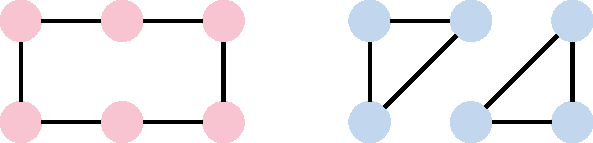
\includegraphics[width=\linewidth]{figures/tikz_WL.pdf} 一个简单例子：WL 检验无法区分\emph{六元环}与\emph{两个三角形}。}而且有许多它无法区分非同构图的简单例子，但其表达能力最终与 GNN 紧密相关。\citet{morris2019weisfeiler} 和 \citet{xu2018powerful} 的分析都得出了一个惊人的结论：符合第 \ref{sec:gnn-intro} 节所述三种类型之一的\emph{任何} GNN，其能力都不可能超过 WL 检验！

要准确达到这一表示能力水平，必须对 GNN 更新规则施加某些约束。\citet{xu2018powerful} 表明，在离散特征域中，GNN 使用的聚合函数必须是\emph{单射的}，而\emph{求和}是一个关键代表。\marginnote{最大化和平均等常见聚合器在这一点上有所不足，因为它们无法区分例如邻居多重集 $\ldblbrace \vec{a}, \vec{b}\rdblbrace$ 与 $\ldblbrace \vec{a}, \vec{a}, \vec{b}, \vec{b}\rdblbrace$。}根据分析结果，\citet{xu2018powerful} 提出了 Graph Isomorphism Network（GIN）；它是该框架下具有最大表达能力的一个简单而强大的 GNN 实例，也可以用我们提出的卷积 GNN 类型表达。

最后值得注意的是，这些发现不能推广到\emph{连续}节点特征空间。事实上，\citet{corso2020principal} 利用 Borsuk--Ulam 定理 \citep{borsuk1933drei} 证明，在假定节点特征为实值时，得到单射聚合函数需要\emph{多个}聚合器（具体而言，其数量等于接收节点的\emph{度}）。\marginnote{这类聚合器的一个例子是邻居多重集的\emph{矩}。}他们的发现推动了 Principal Neighbourhood Aggregation（PNA）架构；该架构提出了一个经验上强大且稳定的多聚合器 GNN。

\paragraph{高阶方法} % and Topological Data Analysis}

前几段的发现并不否定 GNN 的实际效用。事实上，在许多现实应用中，输入特征足够\emph{丰富}，尽管存在上述限制，仍能支持对图结构进行有用的判别计算。\marginnote{相比之下，上述限制几乎总是针对\emph{无特征}或\emph{带类别特征}的图。}

不过，一个重要推论是，GNN 在检测图内某些基本\emph{结构}方面相对较弱。在 WL 检验的具体局限或失败案例引导下，多项工作提出了\emph{更强的} GNN 变体；可以\emph{证明}它们比 WL 检验更强，因此很可能适用于需要这类结构检测的任务。\marginnote{一个突出实例是计算化学：分子图中是否存在芳香\emph{环}，可能强烈影响分子的化学功能。}

寻找表达能力更强的 GNN，最直接的地方或许就是 WL 检验本身。事实上，可以考虑 WL 检验的\emph{层次体系}来增强原始 WL 检验，使 $k$-WL 检验为节点的 $k$\emph{-元组}赋予表示 \citep{morris2017glocalized}。\citet{morris2019weisfeiler} 把 $k$-WL 检验直接转化为\emph{高阶} $k$-GNN 架构；\marginnote{已有一些工作采用 $\delta$-$k$-LGNN \citep{morris2020weisfeiler} 等方法，尝试稀疏化 $k$-GNN 的计算。}可以证明，该架构比此前考虑的 GNN 类型更强。然而，它必须维护元组表示，这意味着实践中很难扩展到 $k=3$ 以上。

与此同时，\citet{maron2018invariant,maron2019provably} 研究了节点 $k$-元组上的不变与等变图网络的刻画。他们不仅证明了一个令人惊讶的结果——\emph{任意}不变或等变图网络都可以表示为有限个生成元的线性组合，而生成元数量仅依赖于 $k$——还证明了这类层的表达能力等价于 $k$-WL 检验，并提出一种经验上可扩展且可证明具有 3-WL 能力的变体。

除了推广计算表示的域之外，大量工作还用于分析 1-WL 的具体失败案例，并扩充 GNN 的\emph{输入}，以帮助模型区分这些情形。一个常见例子是为节点附加\emph{标识特征}，这有助于检测结构。\marginnote{例如，如果一个节点在 $k$ 跳之外看到自己的标识符，就直接说明它位于一个 $k$-环内。}相关方案包括 \emph{one-hot} 表示 \citep{murphy2019relational}，以及纯\emph{随机}特征 \citep{sato2020random}。

更广泛地说，已有许多工作尝试在消息传递过程中纳入\emph{结构}信息，或者调节消息函数，或者调节承载计算的图。\marginnote{在计算化学领域，人们常假定分子功能由子结构（即\emph{官能团}）驱动；这直接启发了在\emph{基元}层面对分子建模。相关参考文献见 \cite{jin2018junction,jin2020hierarchical,fey2020hierarchical}。}其中一些有趣的研究方向包括采样\emph{锚节点集合} \citep{you2019position}、基于\emph{Laplacian 特征向量}聚合 \citep{stachenfeld2020graph,beaini2020directional,dwivedi2020generalization}，以及执行\emph{拓扑数据分析}，将其用于位置嵌入 \citep{bouritsas2020improving} 或驱动消息传递 \citep{bodnar2021weisfeiler}。

 
% Lastly, it is important to note that one of the most popularised and impactful applications of graph representation learning at the time of writing this book exactly corresponds to using GNNs to accurately screen potential drugs, leading to discovery of a novel potent antibiotic, Halicin \citep{stokes2020deep}. 

%\michael{
\paragraph{信号处理与调和分析}
自卷积神经网络早期取得成功以来，研究者便借助调和分析、图像处理和计算神经科学中的工具，尝试提供一个能够解释其效率的理论框架。
$M$-理论是一个受视觉皮层启发的框架，由 Tomaso Poggio 及其合作者 \citep{riesenhuber1999hierarchical, serre2007feedforward} 开创，基于可在某些对称群下操纵的模板概念。计算神经科学中产生的另一个重要模型是\emph{可转向金字塔}；它由 \cite{simoncelli1995steerable} 提出，是一种对某些输入变换具有良好性质的多尺度小波分解。可转向金字塔是早期纹理生成模型 \citep{portilla2000parametric} 的核心元素；随后，人们用深度 CNN 特征取代可转向小波特征，改进了这些模型 \cite{gatys2015texture}。
最后，由 St{\'e}phane \cite{mallat2012group} 引入、并由 \cite{bruna2013invariant} 发展的散射变换，通过用多尺度小波分解取代可训练滤波器，为理解 CNN 提供了一个框架，同时展示了形变稳定性以及深度在架构中的作用。


% Wavelets Mallat

% Multiscale analysis

% Simoncelli

% Poggio
%}


%[spectral]

\paragraph{图与网格曲面上的信号处理}
另一类重要的图神经网络通常称为\emph{谱方法}；它源于本文一位作者的工作 \citep{bruna2013spectral}，并采用\emph{图 Fourier 变换}这一概念。
%
这一构造源自信号处理与计算调和分析研究群体；在 2000 年代末和 2010 年代初，处理非 Euclidean 信号在这些领域中日益受到重视。Pierre Vandergheynst 团队 \citep{shuman2013emerging} 和 Jos{\'e} Moura 团队 \citep{sandryhaila2013discrete} 的有影响力论文普及了“图信号处理”（GSP）概念，以及基于图邻接矩阵与 Laplacian 矩阵特征向量的 Fourier 变换推广。
%
\citet{defferrard2016convolutional} 和 \cite{kipf2016semi} 提出的依赖谱滤波器的图卷积神经网络，是该领域被引用最多的工作之一，也很可能重新点燃了近年来人们对图上机器学习的兴趣。


值得注意的是，在计算机图形学与几何处理领域，非 Euclidean 调和分析比图信号处理至少早十年。流形与网格曲面上的谱滤波器可以追溯到 \cite{taubin1996optimal} 的工作。进入 2000 年代后，随着%Zachi Karni and Craig Gotsman
\cite{karni2000spectral} 关于谱几何压缩的有影响力论文，以及 \cite{levy2006laplace} 关于把 Laplacian 特征向量用作非 Euclidean Fourier 基的工作，这些方法进入主流。
%
谱方法已被用于多种应用，\marginnote{Roee Litman 和 Alex Bronstein（\citeyear{litman2013learning}）提出了与谱图 CNN 类似的可学习形状描述符；后者是本文一位作者的孪生兄弟。}其中最突出的是构造形状描述符 \citep{sun2009concise} 和函数映射 \citep{ovsjanikov2012functional}；在本文写作时，这些方法仍广泛用于计算机图形学。


%\michael{Kova\v{c}evi\'{c}}




\paragraph{计算机图形学与几何处理}
%\michael{Metric models, isometry-invariance, symmetry}
计算机图形学与几何处理领域的多位作者提出了基于内蕴度量不变量的形状分析模型 \citep{elad2003bending,memoli2005theoretical,bronstein2006generalized}；本文一位作者在其早期著作中对此作了深入讨论 \citep{bronstein2008numerical}。同一领域还研究了内蕴对称性的概念 \cite{raviv2007symmetries,ovsjanikov2008global}。
%
首个网格曲面深度学习架构 Geodesic CNN，由本文一位作者所在的团队开发 \citep{masci2015geodesic}。该模型使用具有共享权重的局部滤波器，并将其应用于沿测地线定义的径向斑块。它是本文另一位作者后来开发的规范等变 CNN \citep{cohen2019gauge} 的一种特殊设置。
%
同一团队的 Federico \cite{monti2017geometric} 提出了 Geodesic CNN 的推广 MoNet，采用可学习的聚合运算。MoNet 在网格曲面的局部结构特征上使用类似注意力的机制，并已被证明同样适用于一般图。
%
图注意力网络（GAT）由本文另一位作者提出 \citep{velickovic2018graph}；从技术上说，它可以视为 MoNet 的一个特殊实例。GAT 把 MoNet 的注意力机制推广到同时纳入节点特征信息，从而突破了先前工作中相关性纯粹源于结构的限制。它是目前最流行的 GNN 架构之一。


在计算机图形学背景下，还值得一提的是，集合上学习的思想 \citep{zaheer2017deep} 同时也由 Stanford 的 Leo Guibas 团队以 PointNet 之名发展，用于分析 3D 点云 \citep{qi2017pointnet}。该架构催生了多项后续工作，其中包括本文一位作者提出的 Dynamic Graph CNN（DGCNN，\cite{wang2019dynamic}）。DGCNN 使用最近邻图捕获点云的局部结构，使信息能够在节点之间交换；该架构的关键特征是即时构造图，并根据下游任务在神经网络各层之间更新图。
%
后一项性质使 DGCNN 成为“潜在图学习”最早的实现形式之一，而这一方向随后得到了大量后续研究。对 DGCNN 的 $k$ 最近邻图方案的推广，包括通过双层优化 \citep{franceschi2019learning}、强化学习 \citep{kazi2020differentiable} 或直接监督 \citep{velivckovic2020pointer}，更明确地控制这些图的边。与此独立地，NRI 模型 \citep{kipf2018neural} 开启了一个变分方向，即从计算得到的\emph{后验}分布中以概率方式采样边。尽管它仍依赖关于节点数的二次计算，却能显式编码所选边的不确定性。
%\michael{Mention algorithmic reasoning and Cranmer's work on symbolic equations?}

在没有给定图的情况下进行图上学习，另一个非常流行的方向是在\emph{完全图}上执行 GNN 式计算，让网络自行推断利用连通性的方式。这一需求在自然语言处理中尤为突出，因为句子中的不同词语以高度非平凡且非顺序的方式相互作用。在词语完全图上进行运算，促成了 Transformer 模型的最初实现 \citep{vaswani2017attention}；它取代循环模型和卷积模型，成为神经机器翻译的最先进方法，并掀起了跨越 NLP 与其他领域边界的大量相关工作。全连接 GNN 计算也同时出现在仿真 \citep{battaglia2016interaction}、推理 \citep{santoro2017simple} 和多智能体 \citep{hoshen2017vain} 应用中；当节点数相对较小时，它至今仍是一种流行选择。
%
%Most recent works 

%manifold learning 

%Rotation-equivariant CNNs

\paragraph{算法推理}
在本节的大部分讨论中，我们给出的例子都是由\emph{空间}诱导的几何，它们进而塑造底层域及其不变性与对称性。然而，在\emph{计算}设置中同样存在大量不变性与对称性实例。它与几何深度学习许多常见设置的一项关键区别在于，链接不再需要编码任何相似性、接近程度或关系类型；它们只规定所连接数据点之间数据流的“配方”。

神经网络的计算转而模仿\emph{算法}的推理过程 \citep{cormen2009introduction}，而算法的控制流与中间结果还会诱导出额外的不变性。\marginnote{例如，Bellman--Ford 寻路算法 \citep{bellman1958routing} 的一个不变量是：在 $k$ 步之后，它总能计算出使用不超过 $k$ 条边到达源节点的最短路径。}在算法领域，对输入假定的不变量常称为\emph{前置条件}，而算法所保持的不变量称为\emph{后置条件}。

同名研究方向\emph{算法推理} \citep[Section 3.3.]{cappart2021combinatorial} 旨在构造能够适当保持算法不变量的神经网络架构。该领域研究了通用神经计算机的构造，例如 \emph{neural Turing machine} \citep{graves2014neural} 和 \emph{differentiable neural computer} \citep{graves2016hybrid}。尽管这类架构具备通用计算的所有特征，但它们一次引入多个组件，因而往往难以优化；实践中，\citet{santoro2017simple,santoro2018relational} 所提出的简单关系推理器几乎总能超过它们。

由于建模复杂后置条件颇具挑战性，关于学习执行的归纳偏置研究 \citep{zaremba2014learning} 大多聚焦于基本算法（例如简单算术）。该领域的突出实例包括 \emph{neural GPU} \citep{kaiser2015neural}、\emph{neural RAM} \citep{kurach2015neural}、\emph{neural programmer-interpreters} \citep{reed2015neural}、\emph{neural arithmetic-logic units} \citep{trask2018neural,madsen2020neural} 和 \emph{neural execution engines} \citep{yan2020neural}。

GNN 架构的快速发展使模拟具有\emph{超线性}复杂度的组合算法成为可能。\citet{xu2019can} 开创的\emph{算法对齐}框架从理论上证明，GNN 与动态规划\emph{对齐} \citep{bellman1966dynamic}，而大多数算法都可以用动态规划这种语言表达。与此同时，本文一位作者从经验上表明，实践中可以设计并训练与算法不变量对齐的 GNN \citep{velivckovic2019neural}。随后，人们实现了与\emph{迭代算法} \citep{tang2020towards}、\emph{线性对数算法} \citep{freivalds2019neural}、\emph{数据结构} \citep{velivckovic2020pointer} 和\emph{持久内存} \citep{strathmann2021persistent} 的对齐。这类模型还在\emph{隐式规划器} \citep{deac2020xlvin} 中得到实际应用，进入了\emph{强化学习}算法领域。

与此同时，使用 GNN 进行\emph{物理仿真}也取得了显著进展 \citep{sanchez2020learning,pfaff2020learning}。这一方向对可泛化 GNN 的设计给出了许多相同建议。这种对应关系并不意外：算法可以表述为离散时间仿真，而仿真通常实现为逐步算法，因此两个方向都需要保持相似类型的不变量。

与算法推理研究紧密相连的是对\emph{外推}的度量。外推是神经网络一个众所周知的痛点，因为多数成功案例都发生在\emph{分布内}泛化时，即训练数据中的模式能够恰当地预示测试数据中的模式。然而，无论输入的大小或生成分布如何，算法不变量都必须得到保持；这意味着训练集很可能无法覆盖实践中遇到的所有可能场景。\citet{xu2020neural} 从几何角度论证了由整流激活支持的外推 GNN 需要满足什么条件：其组件和特征化方式必须经过设计，使组成模块（例如消息函数）只学习\emph{线性}目标函数。\citet{bevilacqua2021size} 提出从\emph{因果推理}视角考察外推，从而得到图的\emph{环境不变}表示。

\paragraph{几何深度学习}
最后的历史评述涉及本文的名称本身。
%
术语“几何深度学习”最早由本文一位作者在其 2015 年 ERC 资助申请中提出，并经 IEEE Signal Processing Magazine 上的同名论文 \citep{bronstein2017geometric} 得到普及。该论文虽然“带着几分谨慎”，却宣称出现了“一个新领域正在诞生”的迹象。鉴于图神经网络近来的流行、不变性与等变性观念在广泛机器学习应用中日益得到采用，以及我们正在撰写本文这一事实，或许可以认为这一预言至少部分实现了。
%
名称“4G: Grids, Graphs, Groups, and Gauges”由 Max Welling 为 ELLIS 几何深度学习项目创造；该项目由本文的两位作者共同主持。必须承认，最后一个“G”多少有些牵强，因为底层结构是流形与丛，而不是规范。
%
在本文中，我们又加入了一个“G”，即 Geodesics，用来指代流形的度量不变量与内蕴对称性。


%{\footnotesize


\section*{致谢}

%Our book 
本文
尝试从不变性与对称性的几何视角出发，对数十年来%geometric
深度学习架构方面的既有知识进行概括与综合。
% 
%
我们希望这一视角
%---largely propelled by inspiration from the Erlangen Program---
既能帮助新手和实践者更轻松地认识这一领域，也能帮助研究者把新架构综合为我们蓝图的实例。从某种意义上说，我们希望已经给出了\emph{“构建那些‘你所需要的一切’架构所需要的一切”}——这是受 \citet{vaswani2017attention} 启发的文字游戏。



%In many ways, the seeds for this text %book 
%have been planted many years before a single paragraph had been written. The four of us had been, perhaps unknowingly, exploring research directions we present here under the title of Geometric Deep Learning for many years.  
%Michael and Joan did it from the lens of signal processing (alongside Yann LeCun, Arthur Szlam and Pierre Vandergheynst), Taco from the lens of group-equivariant convolutions (alongside Mario Geiger, Jonas K\"{o}hler and Max Welling) and Petar through spatial graph representation learning (alongside Yoshua Bengio, Arantxa Casanova, Guillem Cucurull,  Pietro Li\`{o} and Adriana Romero). We deeply thank all of the co-authors listed above, as with their support we produced several pieces of early evidence that the blueprint is worth studying: the first Geometric Deep Learning review paper \citep{bronstein2017geometric} (with highly-attended companion tutorial at NIPS 2017), Spherical CNNs \citep{cohen2018spherical} (best-paper awardee at ICLR 2018) and Graph Attention Networks \citep{velickovic2018graph} (the top-cited paper at ICLR 2018).
%
%The first occasion\marginnote{\includegraphics[width=\linewidth]{figures/Michael.jpeg}\\ \includegraphics[width=\linewidth]{figures/Taco.jpeg}} when all the authors %of our respective work (literally) 
%came together was the Workshop on Representation Learning on Graphs and Manifolds that took place at ICLR  in New Orleans in 2019. Joan and Petar were both co-organisers of the workshop, while Michael and Taco delivered two of the keynote talks on mesh CNNs for protein design and 
%---covering topics of geometric deep learning (for protein design), and 
%gauge-equivariant convolutions,  respectively. 
%Both of these topics feature prominently in this writeup. We would like to thank the entire co-organising team of this workshop (Pete Battaglia, Albert Gu, Beliz Gunel, Will Hamilton, Thomas Kipf, Yujia Li, Max Nickel, Razvan Pascanu, Chris R\'{e}, Adriana Romero, Fred Sala and Marinka \v{Z}itnik), the ICLR 2019 organisers for giving us the opportunity to host such a workshop, and consequently allow us to discuss these topics in the same space.
%\petar{We thank the IAS...}
%
%Though probably each of us had been dreaming of writing at some point a ``deep learning textbook that would not become obsolete by the time of its publication'', the concrete steps towards this project were taken by Joan. 
%
%The first outline was drafted in February 2020 by Joan and Michael while both were visitors at the Institute for Advanced Studies in Princeton (a kind invitation for which we are grateful to Sanjeev Arora). This also happened to be the last in-person meeting, as the start of the coronavirus pandemic made Zoom calls the new normal and also introduced some corrections into the original schedule. 



本文的大部分内容写于 2020 年末至 2021 年初。与此类工作中常见的情形一样，我们无数次怀疑这幅整体图景是否合理，并借助同事提供的机会
%
%Ultimately, we are grateful to all of the venues that 
克服“怯场”，展示工作早期版本；这些工作最初
%to wider \emph{Zoom} audiences. 
%In many ways, our work first saw the 
通过 Petar 在 Cambridge 的演讲（承蒙 Pietro Li{\`o} 邀请），以及 Michael 在 Oxford（承蒙 Xiaowen Dong 邀请）和 Imperial College（由 Michael Huth 与 Daniel Rueckert 主持）的演讲与公众见面。应 Andreas Maier 的盛情邀请，Petar 还得以在 Erlangen Programme 的诞生地 Friedrich-Alexander-Universit\"{a}t Erlangen-N\"{u}rnberg 展示我们的工作！
%
%
%through Michael's talks on \emph{``Geometric Deep Learning''}\marginnote{Michael's GDL talks came with various subtitles---\emph{``GDL for 3D human body synthesis''}, \emph{``GDL, from Euclid to drug design''}, and \emph{``GDL: the Erlangen Programme of ML''}.} and Petar's talk on \emph{``Theoretical Foundations of Graph Neural Networks''}, and 
这些演讲收到的反馈极其宝贵，既鼓舞了我们的士气，也帮助我们进一步打磨了这项工作。
%Accordingly, we thank the organisers of the \emph{Topological Data Analysis and Beyond} Workshop at NeurIPS 2020, \emph{University of Cambridge}, and \emph{Imperial College London}. 
最后同样重要的是，我们感谢 ICLR 2021 组委会；Michael 将在该会议的主题演讲中介绍我们的工作。

%Karsten Bogwart review on graph kernels

%}

需要指出的是，
仅凭四个人的专业知识，通常不足以协调如此庞大的研究成果。因此，我们希望向所有在本文演进过程中认真研读其不同方面，并提供细致意见和参考文献的研究者致以应有的谢意：Yoshua Bengio、Charles Blundell、Andreea Deac、Fabian Fuchs、Francesco di Giovanni、Marco Gori、Raia Hadsell、Will Hamilton、Maksym Korablyov、Christian Merkwirth、Razvan Pascanu、Bruno Ribeiro、Anna Scaife、J\"{u}rgen Schmidhuber、Marwin Segler、Corentin Tallec、Ng\^{a}n V\~{u}、Peter Wirnsberger 和 David Wong。他们的专业反馈对于巩固我们的统一化工作、使其更适用于各个细分领域极为宝贵。当然，本文中的任何不妥之处均由我们自行负责。当前工作仍在持续完善中，我们非常欢迎在任何阶段收到意见；若发现任何错误或遗漏，敬请与我们联系。


% Chinese-reader supplement: not part of the English source manuscript.
\renewcommand{\appendixname}{附录}
\appendix
\chapter{数学概念导读：从深度学习实例理解几何结构}
\label{app:primer:chapter}

\begin{tcolorbox}[width=\linewidth,colback=boxgray!45,colframe=darkgry,title=附录身份与使用方式]
本章是为中文版读者编写的编辑性增补，不属于英文原稿，也不代表原作者新增的论述。它面向熟悉基础深度学习、向量和矩阵运算，但尚未系统学习抽象代数或微分几何的读者。目标不是替代数学教材，而是建立一组足以阅读正文的概念支点。建议先阅读本章，再回到第~\ref{sec:geom_priors} 节的几何先验和正文后续各节。
\end{tcolorbox}

几何深度学习中的抽象概念通常围绕同一条设计链展开：先确定数据位于什么\emph{域}上，再确定哪些变换不应改变任务含义，随后规定中间特征在这些变换下应如何变化，最后据此限制网络层的形式。理解这条链，比孤立记忆“群”“流形”或“Laplacian”的定义更有帮助。

\section{先分清四类对象}
\label{app:primer:objects}

阅读公式时，可以先判断每个符号属于以下哪一类。

\begin{center}
\small
\begin{tabular}{@{}p{0.18\linewidth}p{0.34\linewidth}p{0.39\linewidth}@{}}
\toprule
对象 & 它回答的问题 & 深度学习中的典型实例 \\
\midrule
域 $\Omega$ & 数据索引位于哪里，哪些索引彼此相邻 & 图像像素坐标、图节点、曲面上的点 \\
信号 $x$ & 每个索引位置存放什么数值 & RGB 值、节点特征、温度场、3D 向量特征 \\
变换 $\fg$ & 哪种改变应被视为同一对象的另一种观察方式 & 图像平移、节点重编号、3D 旋转 \\
模型 $F$ & 输入改变后，输出应保持不变还是同步改变 & 分类器、分割器、节点预测器 \\
\bottomrule
\end{tabular}
\end{center}

集合只说明“有哪些元素”，本身不提供顺序、距离或线性运算。例如，点云可以首先看作点的集合。映射 $x:\Omega\rightarrow\mathcal{C}$ 给每个域元素 $u\in\Omega$ 指定一个值 $x(u)\in\mathcal{C}$，因此把“位置”和“位置上的特征”分开了。向量空间则额外允许向量加法与标量乘法；像素的 RGB 通道或节点的隐藏特征通常位于某个向量空间中。

\begin{tcolorbox}[width=\linewidth,colback=boxgray!35,colframe=darkgry,title=深度学习实例：同一个矩阵可能承担不同角色]
图像可以写成矩阵，但矩阵的行列顺序与二维像素坐标绑定。图的节点特征也可以写成矩阵 $\vec{X}\in\mathbb{R}^{n\times s}$，但它的行顺序只是节点编号；同时重排节点特征和邻接矩阵，不应改变图本身。

\textbf{它说明什么：}数组表示不等于几何结构，必须同时说明索引域及其允许的变换。

\textbf{它没有说明什么：}并非所有矩阵都能任意重排行列；对图像像素任意置换通常会破坏空间邻接关系。
\end{tcolorbox}

\section{群、群作用与群表示}
\label{app:primer:groups}

\subsection{群：可以一致地复合和撤销的变换}

群 $\fG$ 是带有复合运算的集合。该运算满足结合律；群中存在单位元 $e$；每个元素 $\fg$ 都有逆元 $\fg^{-1}$。这里的重点不是“元素看起来像什么”，而是变换能否复合、是否有“不做任何事”的变换，以及能否撤销。

整数平移构成群：先平移 $a$ 个像素再平移 $b$ 个像素，等价于平移 $a+b$ 个像素；零平移是单位元；平移 $a$ 的逆变换是平移 $-a$。固定大小集合上的所有置换也构成群，但其复合通常不满足交换律。

\subsection{群作用：变换如何移动数据的位置}

仅有群还不够，必须说明群元素如何作用于具体域。群作用写成 $\fg.u$，并满足
\begin{equation}
e.u=u,
\qquad
(\fg_1\fg_2).u=\fg_1.(\fg_2.u).
\label{app:primer:group-action}
\end{equation}
例如，二维整数平移群可以作用于像素坐标，置换群可以作用于图的节点编号。相同的抽象群也可能以不同方式作用于不同对象，因此“群”和“群作用”不能混用。正文第~\ref{sec:symmetries} 节及式~\plaineqref{eq:group_action} 给出了更完整的讨论。

\subsection{群表示：变换如何作用于特征向量}

群表示把群元素映射为可逆线性算子：
\begin{equation}
\rho:\fG\rightarrow\mathrm{GL}(V),
\qquad
\rho(\fg_1\fg_2)=\rho(\fg_1)\rho(\fg_2).
\label{app:primer:representation}
\end{equation}
它描述特征坐标随变换如何变化。标量亮度在旋转图像时通常不需要旋转自身；二维方向向量则应随图像旋转。二者可以对应同一旋转群的不同表示。

\begin{tcolorbox}[width=\linewidth,colback=boxgray!35,colframe=darkgry,title=常见误解：群作用不是群表示]
群作用首先描述域元素如何移动，例如像素位置 $u$ 变成 $\fg.u$；群表示描述向量特征如何线性变换，例如方向通道乘以旋转矩阵。对标量图像，两者容易在记号上显得相似；对向量场或张量特征，它们的区别不可省略。
\end{tcolorbox}

\section{不变性与等变性：模型输出应该怎样响应}
\label{app:primer:invariance-equivariance}

设 $\rho_{\mathrm{in}}(\fg)$ 表示变换在输入上的作用。若任务输出不应随变换改变，则模型 $F$ 应满足不变性：
\begin{equation}
F(\rho_{\mathrm{in}}(\fg)x)=F(x).
\label{app:primer:invariance}
\end{equation}
若输出也有相应的变换规则 $\rho_{\mathrm{out}}(\fg)$，则希望满足等变性：
\begin{equation}
F(\rho_{\mathrm{in}}(\fg)x)
=\rho_{\mathrm{out}}(\fg)F(x).
\label{app:primer:equivariance}
\end{equation}

图像分类通常希望对小范围平移近似不变：猫移到画面另一位置，类别仍是“猫”。语义分割则不同：输入向右平移后，输出掩码也应向右平移，因此中间和最终的空间输出更适合满足平移等变性。规则网格上的卷积层是经典的平移等变构造；群卷积把这一思想推广到更一般的群作用 \citep{cohen2016group}。

\begin{center}
\small
\begin{tabular}{@{}p{0.25\linewidth}p{0.28\linewidth}p{0.38\linewidth}@{}}
\toprule
任务 & 合理目标 & 变换后的期望输出 \\
\midrule
图像分类 & 不变或近似不变 & 类别不变 \\
语义分割 & 等变 & 掩码与图像同步移动 \\
图节点分类 & 置换等变 & 节点输出按同一置换重排 \\
整图分类 & 置换不变 & 图级预测不依赖节点编号 \\
\bottomrule
\end{tabular}
\end{center}

\begin{tcolorbox}[width=\linewidth,colback=boxgray!35,colframe=darkgry,title=边界：数据增强不等于严格等变]
用平移或旋转后的样本训练模型，可能提高模型对这些变换的经验鲁棒性，但有限数据增强通常不能单独证明式~\plaineqref{app:primer:invariance} 或式~\plaineqref{app:primer:equivariance} 对所有输入和所有群元素严格成立。结构性等变来自网络层满足相应代数约束；经验性能还取决于数据、优化和模型容量。
\end{tcolorbox}

正文第~\ref{sec:gdl_blueprint} 节给出了从局部等变层到全局任务输出的设计蓝图。

\section{格、规则网格、网格曲面与一般图}
\label{app:primer:lattices-grids}

“格”和“网格”在不同领域中可能指不同对象。本节中的\emph{格}（lattice）指由一组线性无关基向量生成的离散平移集合，例如
\begin{equation}
\Lambda=\left\{\sum_{i=1}^{d} k_i b_i: k_i\in\mathbb{Z}\right\}.
\label{app:primer:lattice}
\end{equation}
二维方格和六角格都属于这种意义下的格；这里的“格”不是序理论中带有上确界、下确界运算的 lattice。

规则网格通常是格上的有限采样区域，外加固定的邻接方式与边界规则。数字图像是最熟悉的例子：像素坐标近似位于二维方格上，每个内部像素共享相同的局部邻域模板。正是这种全局一致的平移结构，使同一卷积核可以在不同位置共享参数：
\begin{equation}
(x\star\theta)(u)=\sum_v x(v)\theta(u-v).
\label{app:primer:grid-convolution}
\end{equation}

网格曲面（mesh）则通常由顶点、边和面离散表示曲面。它的连接关系可能不规则，不存在覆盖整个曲面的单一平移坐标。因此，图像网格上的卷积核不能直接原样搬到任意网格曲面上。正文第~\ref{sec:grids_euclidean} 节讨论规则网格，第~\ref{sec:meshes} 节讨论流形网格曲面。

\begin{tcolorbox}[width=\linewidth,colback=boxgray!35,colframe=darkgry,title=深度学习实例：为什么 CNN 能共享卷积核]
在图像内部，不同像素的局部邻域可以用同一组相对偏移表示，例如“左一格、右一格、上一格、下一格”。卷积核把权重绑定到这些相对偏移，而不是绑定到绝对像素编号。

\textbf{它说明什么：}参数共享依赖可重复的局部几何模板。

\textbf{它没有说明什么：}图像边界、非均匀采样和任意图不自动拥有相同的平移结构；padding 的选择也会影响边界处的严格等变性。
\end{tcolorbox}

\section{图与消息传递}
\label{app:primer:graphs}

图 $G=(\mathcal{V},\mathcal{E})$ 由节点集合与边集合组成。图结构说明哪些对象直接关联，但一般不提供全局坐标、唯一距离或统一方向。分子中的原子可以作为节点，化学键作为边；社交网络中的用户可以作为节点，关系作为边。

节点编号只是存储约定。若用置换矩阵 $\vec{P}$ 同时重排节点特征和邻接矩阵，则得到的仍是同一张带特征图的不同表示。因此，节点级模型应对这种重编号等变，整图模型则应对其不变。

消息传递 GNN 的一层可以抽象为
\begin{align}
m_u &= \bigoplus_{v\in\mathcal{N}(u)}
      \psi(x_u,x_v,e_{uv}), \\
h_u &= \phi(x_u,m_u),
\label{app:primer:message-passing}
\end{align}
其中 $\mathcal{N}(u)$ 是节点 $u$ 的邻域，$\psi$ 生成邻居消息，$\bigoplus$ 是对邻居顺序不敏感的聚合，$\phi$ 更新节点特征。求和、均值或最大值都是常见的置换不变聚合，但它们保留的信息不同。正文第~\ref{sec:proto-graphs} 节介绍图域，第~\ref{sec:gnn-intro} 节讨论 GNN；消息传递框架的代表性形式见 \citet{gilmer2017neural}。

\begin{tcolorbox}[width=\linewidth,colback=boxgray!35,colframe=darkgry,title=边界：一般图不是弯曲的图像网格]
规则图像网格可以表示为图，因此某些 CNN 操作可以写成图上的局部聚合。但一般图没有统一的“左、右、上、下”，节点度数也可能不同。由此只能推出两者共享局部聚合思想，不能推出任意 GNN 都等价于 Euclidean CNN。
\end{tcolorbox}

集合模型可看作图结构的一个极端情形：只要求元素置换不改变集合含义，而不指定成对边。Deep Sets 使用逐元素映射与对称聚合构造置换不变函数 \citep{zaheer2017deep}。

\section{度量、拓扑与流形}
\label{app:primer:manifolds}

\subsection{度量告诉我们“多远”，拓扑告诉我们“多近才算邻近”}

度量空间在集合 $\Omega$ 上配备距离 $d(u,v)$。距离满足非负性、同一性、对称性与三角不等式。度量允许定义最近邻、球和曲线长度。拓扑保留更弱的信息：哪些集合是开集、哪些序列收敛、函数是否连续。不同度量可能诱导同一拓扑，因此“连续性结构相同”不意味着实际距离相同。

在深度学习中，最近邻图的构造依赖所选度量。若把点云坐标从米改成各轴不同的缩放，Euclidean 最近邻关系可能改变；这不是模型实现细节，而是数据几何假设的一部分。

\subsection{流形在局部像 Euclidean 空间}

一个 $d$ 维流形在每个点附近都可以用 $\mathbb{R}^d$ 中的局部坐标描述，但全局上未必存在单一坐标系。球面局部像二维平面，却不能无失真地铺成一张全局平面图。流形可能嵌入更高维空间；嵌入空间中的直线距离是外在量，沿流形的最短路径长度是内蕴量，二者通常不同。

点云是离散样本，网格曲面是带连接关系的离散近似；它们本身不因“看起来像曲面”就自动满足所假设流形的全部光滑性质。模型使用切空间、测地线或曲率时，通常还依赖采样密度、离散化和数值近似。

\subsection{切空间是局部线性化}

点 $u$ 处的切空间 $T_u\Omega$ 收集经过 $u$ 的曲线在该点的速度方向。它把局部非线性几何转化为可做线性代数的空间。Riemann 度量 $g_u$ 在每个切空间上给出内积，从而定义向量长度与夹角，并进一步定义曲线长度和测地距离。

\begin{tcolorbox}[width=\linewidth,colback=boxgray!35,colframe=darkgry,title=深度学习实例：曲面上的方向特征]
人体表面网格上的每个顶点可以带一个切向量特征，例如沿表面的运动方向。不同顶点的切空间不同，两个向量不能只凭坐标分量直接相加；必须先规定如何把一个点的方向与另一个点的方向比较。

\textbf{它说明什么：}曲面网络需要处理局部坐标与跨点比较问题。

\textbf{它没有说明什么：}并非每项 3D 任务都必须使用完整微分几何；若任务只使用标量或距离，所需结构可能更少。
\end{tcolorbox}

正文第~\ref{sec:geomanifoldsec} 节引入流形，第~\ref{sec:manifolds} 节讨论度量与分析工具。

\section{Laplacian、谱与 Fourier 观点}
\label{app:primer:laplacian}

Laplacian 可以直观理解为衡量一个位置与其邻域聚合状态之差的一类算子；它有组合、归一化等多种形式。在无向加权图上，令 $\vec{A}$ 为对称邻接矩阵，$\vec{D}$ 为度矩阵，则组合 Laplacian 为
\begin{equation}
\vec{L}=\vec{D}-\vec{A}.
\label{app:primer:graph-laplacian}
\end{equation}
对节点标量信号 $\vec{x}$，有
\begin{equation}
\vec{x}^{\top}\vec{L}\vec{x}
=\frac{1}{2}\sum_{u,v}A_{uv}(x_u-x_v)^2.
\label{app:primer:dirichlet-energy}
\end{equation}
因此，当相邻节点取值接近时，该能量较小。这个等式依赖 $\vec{A}$ 对称且权重非负；有向图或带符号图需要不同处理。

若 $\vec{L}\varphi_k=\lambda_k\varphi_k$，则特征向量 $\varphi_k$ 给出一组图信号方向。较小的 $\lambda_k$ 通常对应沿图边变化较慢的模式，较大的 $\lambda_k$ 对应更快速的变化。把信号投影到这些特征向量上，可得到一种图 Fourier 表示。谱滤波器可写成 $p(\vec{L})\vec{x}$；多项式形式不需要显式计算完整特征分解，并具有局部传播解释。谱图卷积网络的早期实例包括 \citet{defferrard2016convolutional}。

在规则周期网格上，普通 Fourier 基能够对角化平移不变卷积；图 Laplacian 的特征基提供了相似的谱语言。但“相似”不等于“完全相同”：任意图上没有唯一平移群，重复特征值对应的特征向量也不唯一，不同图之间的谱基未必自然对齐。正文式~\plaineqref{eq:mesh_lap} 给出网格 Laplacian，式~\plaineqref{eqn:conv_spectral} 讨论谱滤波。

\begin{tcolorbox}[width=\linewidth,colback=boxgray!35,colframe=darkgry,title=常见误解：低频不等于语义上重要]
Laplacian 的“低频”只表示相对于所选图结构和权重变化缓慢。若图边没有表达任务相关关系，低频平滑可能抹去有用信号。谱平滑是一种归纳偏置，而不是普遍正确的语义假设。
\end{tcolorbox}

\section{表示与规范：坐标变化时特征如何变化}
\label{app:primer:gauge}

流形上的局部切空间需要选择基才能把几何向量写成坐标。对每个点分别选择一组局部基，称为选择一个规范。规范变换改变的是局部基，而不是几何对象本身；同一个切向量在新基下会有不同坐标。

若点 $u$ 处的基发生变换 $h_u\in\fG$，向量坐标可能按群表示变化：
\begin{equation}
c'_u=\rho(h_u)c_u.
\label{app:primer:gauge-change}
\end{equation}
一个规范等变层应保证：先改变所有局部基再运行网络，与先运行网络再按相应规则变换输出，得到一致结果。这样，网络结论不依赖任意的坐标选择。

\begin{tcolorbox}[width=\linewidth,colback=boxgray!35,colframe=darkgry,title=深度学习实例：网格曲面上的方向卷积]
在每个网格顶点选择一个局部二维坐标标架，便可描述滤波器方向和切向量通道。换一组坐标标架后，滤波器与特征分量都必须按一致规则变化；否则网络输出会依赖人为选取的“局部横轴”。

\textbf{它说明什么：}规范等变性用于消除局部坐标选择对计算结果的任意影响。

\textbf{它没有说明什么：}规范变换不是把物体在现实空间中旋转；它首先是同一几何对象的坐标描述变化。规范等变性也不意味着输出对所有物理变换都不变。
\end{tcolorbox}

正文第~\ref{sec:gauges} 节给出规范、结构群和规范等变卷积的正式构造。

\section{不变性之外：为什么还需要稳定性}
\label{app:primer:stability}

不变性处理“某类变换不应改变结果”，但现实输入还会受到噪声、采样误差和不属于精确对称群的小形变。稳定性要求小输入变化不会造成失控的输出变化。最基本的形式是 Lipschitz 条件：
\begin{equation}
\lVert F(x)-F(x')\rVert
\leq C\lVert x-x'\rVert.
\label{app:primer:lipschitz}
\end{equation}
常数 $C$ 控制扰动被放大的上界。实际问题中，输入差异可能需要用与域结构相适应的距离衡量，例如图形变、点云匹配或沿流形的形变代价；直接使用坐标逐项差异未必反映语义接近程度。

精确不变、近似不变与稳定是不同性质。分类器可以对整数像素平移严格不变，却对一个像素的对抗扰动不稳定；也可以对小旋转经验上稳定，却不满足任何精确旋转不变公式。正文第~\ref{sec:geom_stab} 节讨论形变稳定性。

\section{带着问题回到正文}
\label{app:primer:reading-guide}

遇到正文中的新算子或网络层时，可以依次回答：

\begin{enumerate}
\item 域 $\Omega$ 是规则网格、集合、图、流形，还是这些结构的离散近似？
\item 输入信号是标量、向量、张量，还是节点/边/面的组合特征？
\item 哪些变换被视为保持任务含义的对称性？这些变换是否真的构成群？
\item 变换作用在域、信号坐标还是二者之上？相应群表示是什么？
\item 任务需要不变输出还是等变输出？是精确性质还是经验近似？
\item 网络层使用了什么局部邻域，聚合是否依赖任意编号或坐标选择？
\item 距离、Laplacian 或谱基来自哪种几何假设？边界条件是什么？
\item 结论依赖哪些离散、连续、有限或光滑性前提？
\end{enumerate}

\begin{center}
\small
\begin{tabular}{@{}p{0.23\linewidth}p{0.34\linewidth}p{0.34\linewidth}@{}}
\toprule
若主要困惑是 & 先复习本附录 & 再阅读正文 \\
\midrule
“变换究竟作用于什么” & 第~\ref{app:primer:groups}、\ref{app:primer:invariance-equivariance} 节 & 第~\ref{sec:symmetries}、\ref{sec:gdl_blueprint} 节 \\
“图像、图和网格为何不同” & 第~\ref{app:primer:lattices-grids}、\ref{app:primer:graphs} 节 & 第~\ref{sec:grids_euclidean}、\ref{sec:proto-graphs} 节 \\
“曲面为何需要局部坐标” & 第~\ref{app:primer:manifolds}、\ref{app:primer:gauge} 节 & 第~\ref{sec:manifolds}、\ref{sec:gauges} 节 \\
“谱卷积在做什么” & 第~\ref{app:primer:laplacian} 节 & 式~\plaineqref{eq:mesh_lap}、\plaineqref{eqn:conv_spectral} \\
“鲁棒与不变是否相同” & 第~\ref{app:primer:stability} 节 & 第~\ref{sec:geom_stab} 节 \\
\bottomrule
\end{tabular}
\end{center}

本章提供的是阅读坐标，而不是绕开定义的捷径。直觉例子用于确定符号扮演的角色；当正文结论依赖精确条件时，仍应以正文给出的定义、假设和公式为准。


\bibliographystyle{plainnat}
\bibliography{references}





\end{document}                          % The required last line
